% arara: pdflatex
% arara: makeindex
% arara: pdflatex
\documentclass[a4paper,10pt]{article}%

\usepackage[hidelinks]{hyperref}
\hypersetup{
%  colorlinks,
  linktoc=page
}
\usepackage{bookmark}


\input{commands.tex}%

\usepackage{showkeys}

\author{Peter Bonventre, Lu\'is A. Pereira}%
\title{Genuine equivariant operads}%

\usepackage{stmaryrd}

\usepackage{upgreek}
\usepackage{mathtools}

\usepackage{geometry}

\usepackage{tikz}%
\tikzset{%
  treenode/.style = {shape=rectangle, rounded corners,%
                     draw, align=center,%
                     top color=white, bottom color=blue!20},%
  root/.style     = {treenode, font=\Large, bottom color=red!30},%
  env/.style      = {treenode, font=\ttfamily\normalsize},%
  dummy/.style    = {circle,draw,inner sep=0pt,minimum size=2mm}%
}

\usetikzlibrary[decorations.pathreplacing,patterns,cd]
% \usetikzlibrary{external}\tikzexternalize
% \makeatletter
% \renewcommand{\todo}[2][]{\tikzexternaldisable\@todo[#1]{#2}\tikzexternalenable}
% \makeatother



% ---------- notational index ----------
% \usepackage[intoc]{nomencl}
% \makenomenclature
% \renewcommand{\nomname}{Notational Index} 
% \renewcommand{\nompreamble}{The following list describes several symbols and maps that are used within the body of the article.}

% \usepackage{etoolbox}
% \renewcommand\nomgroup[1]{%
%   \item[\bfseries
%   \ifstrequal{#1}{C}{Categories}{%
%   \ifstrequal{#1}{M}{Morphisms}{%
%   \ifstrequal{#1}{O}{Other}{}}}%
% ]}
 
% % This will add the units
% \newcommand{\nomunit}[1]{%
% \renewcommand{\nomentryend}{\hspace*{\fill}#1}}

\usepackage{imakeidx}
\makeindex[columns=3, title=Glossary of Notation, intoc]
 




\begin{document}	\maketitle%



\abstract{We build new algebraic structures, which we call genuine equivariant operads and which can be thought of as a hybrid between operads and coefficient systems.
We then prove an Elmendorf-Piacenza type theorem stating that equivariant operads, with their graph model structure, are equivalent to genuine equivariant operads, with their projective model structure.

As an application, we build explicit models for the $N_{\infty}$-operads of Blumberg and Hill.}


\tableofcontents

\section{Introduction}


A surprising feature of topological algebra is that
the category of (connected) topological commutative monoids is quite small,
consisting only of products of Eilenberg-MacLane spaces (e.g. \cite[4K.6]{Hatcher}).
Instead, the more interesting structures are
those monoids which are commutative and associative only up to homotopy and, moreover, up to ``all higher homotopies''.
To capture these more subtle algebraic notions, Boardman-Vogt \cite{BV73} and May \cite{May72} developed
the theory of \textit{operads}\index{categories!Operad@$\O \in \Op(\V)$}.
Informally, an operad $\O$ consists of
sets/spaces $\O(n)$ of ``$n$-ary operations'' carrying a $\Sigma_n$-action recording
``reordering the inputs of the operations'',
and a suitable notion of ``composition of operations''.
The purpose of the theory is then the study of 
``objects $X$ with operations indexed by $\O$'',
referred to as \textit{algebras}, with the notions of monoid, commutative monoid, Lie algebra, algebra with a module, and more,
all being recovered as algebras over some fixed operad in an appropriate category.
Of special importance are the 
$E_\infty$-operads, introduced by 
May in \cite{May72}, which are 
``homotopical replacements'' for the commutative operad
 and encode the aforementioned
 ``commutative monoids up to homotopy''.
In particular, while an
 $E_\infty$-algebra structure on $X$ does not specify unique maps $X^n \to X$, 
 it nonetheless specifies such maps ``uniquely up to homotopy''.
%Moreover, May showed that these operads encoded infinite loop spaces (and hence connective spectra). 

$E_\infty$-operads are characterized by the homotopy type of their levels $\O(n)$: $\O$ is $E_\infty$ if and only if each $\O(n)$ is $\Sigma_n$-free and contractible, i.e., for each subgroup $\Gamma \leq \Sigma_n$ one has
\[
%\mbox{For $\Gamma \leq \Sigma_n$,} \qquad 
\O(n)^\Gamma \sim
\begin{cases}
        * & \text{if } \Gamma = \{*\} , \\
        \varnothing \qquad & \text{otherwise.}
\end{cases}
\]
% Operads encode a variety of algebraic structures, such as monoids, commutative monoids or (depending on the ambient category) Lie algebras, $E_n$-algebras, etc. Indeed, all such instances can be regarded as categories of algebras for some (fixed) suitable operad.
% Informally, an operad $\O$ consists of ``sets/spaces of $n$-ary operations'' $\O(n)$, $n \geq 0$, each of which carries a $\Sigma_n$-action encoding ``reordering the inputs of the operations'', and a suitable notion of ``composition of operations''.
Notably, when studying the homotopy theory of operads in topological spaces
the preferred notion of weak equivalence is 
usually that of ``naive equivalence'',
with a map of operads 
$\O \to \O'$
deemed a weak equivalence if each of the maps
$\O(n) \to \O'(n)$
is a weak equivalence of spaces
upon forgetting the $\Sigma_n$-actions (e.g. \cite[3.2]{BM03}).
In this context, $E_\infty$-operads are then equivalent to the commutative operad $\mathsf{Com}$
\index{categories!Com@$\mathsf{Com}$}
and, moreover, 
any cofibrant replacement of $\mathsf{Com}$
is $E_{\infty}$.
However, naive equivalences differ from the equivalences in ``genuine equivariant homotopy theory'', where a map of $G$-spaces $X \to Y$ is deemed a $G$-equivalence only if the induced fix point maps $X^H \to Y^H$ are weak equivalences for all $H \leq G$.
This contrast hints at a number of novel subtleties that appear in the study of equivariant operads, which we now discuss.


Firstly, noting that for any finite group $G$, a $G$-operad $\O$ (i.e. an operad $\O$ together with a $G$-action commuting with all the structure)
the $n$-th level $\O(n)$ has a $G \times \Sigma_n$-action,
one might guess that a map of $G$-operads
$\O \to \O'$
should be called a weak equivalence if each of the maps
$\O(n) \to \O'(n)$
is a $G$-equivalence after forgetting the $\Sigma_n$-actions, 
i.e. if the maps
\begin{equation}\label{NAIVEOPEQ EQ}
	\O(n)^H \xrightarrow{\sim} \O'(n)^H, \qquad H \leq G \leq G\times \Sigma_n,
\end{equation}
are weak equivalences of spaces. 
However, the notion of equivalence suggested in (\ref{NAIVEOPEQ EQ}) turns out to not be ``genuine enough''.
To see why, we first consider a homotopical replacement for $\mathsf{Com}$ using this theory: 
%recall that the class of (non-equivariant)
%$E_{\infty}$-operads,
%which are up-to-homotopy replacements for the commutative operad
%$\mathsf{Com}(n)=\**$,
%consists of those operads 
%$\O$ such that:
%\begin{inparaenum}
%	\item[(i)] $\O(n)$ is $\Sigma_n$-free and;
%	\item[(ii)] $\O(n)$ is contractible.
%\end{inparaenum}
if one simply equips an $E_{\infty}$-operad $\O$ with a trivial $G$-action, the resulting $G$-operad has fixed points for each subgroup $\Gamma \leq G \times \Sigma_n$
determined by
\begin{equation}\label{NAIVEGEINFTY EQ}
	\O(n)^{\Gamma} \sim 
\begin{cases}
	\** & \text{if } \Gamma \leq G,
\\
	\emptyset & \text{otherwise}.
\end{cases}
\end{equation}
However, as first noted by Costenoble-Waner \cite{CW91} in their study of equivariant infinite loop spaces,
the \textit{$G$-trivial $E_\infty$-operads} of (\ref{NAIVEGEINFTY EQ}) do not provide 
the correct replacement of $\mathsf{Com}$
 in the $G$-equivariant context. 
 %Instead, %notion of $G$-$E_{\infty}$-operads, by which we mean 
%up-to-homotopy replacements of $\mathsf{Com}$ in the $G$-equivariant context. 
Rather, that replacement is provided instead by the 
\textit{$G$-$E_{\infty}$-operads}, characterized by the fixed point conditions
\begin{equation}\label{GENGEINFTY EQ}
	\O(n)^{\Gamma} \sim 
\begin{cases}
	\** & \text{if } \Gamma \cap \Sigma_n = \{\**\},
\\
	\emptyset & \text{otherwise}.
\end{cases}
\end{equation}
In contrasting 
(\ref{NAIVEGEINFTY EQ}) and (\ref{GENGEINFTY EQ}),
we note that 
the subgroups $\Gamma \leq G \times \Sigma_n$ such that $\Gamma \cap \Sigma_n = \{\**\}$ 
are readily shown to be precisely the graphs of partial homomorphisms 
$G \geq H \to \Sigma_n$,
and that $\Gamma \leq G$ if and only if $\Gamma$ is the graph of a trivial homomorphism. 
As it turns out, the notion of weak equivalence described in (\ref{NAIVEOPEQ EQ}) fails to distinguish
(\ref{NAIVEGEINFTY EQ}) and (\ref{GENGEINFTY EQ}), 
and indeed it is possible
to build maps $\O \to \O'$ where
$\O$ is a $G$-trivial $E_{\infty}$-operad (as in (\ref{NAIVEGEINFTY EQ}))
and $\O'$ is a $G$-$E_{\infty}$-operad 
(as in (\ref{GENGEINFTY EQ})).
Therefore, in order to differentiate such operads, one needs to replace the notion of weak equivalence in (\ref{NAIVEOPEQ EQ}) 
with the finer notion of \textit{graph equivalence}, 
so that $\O \to \O'$ is considered a weak equivalence only if
the maps
\begin{equation}\label{GENEOPEQ EQ}
	\O(n)^{\Gamma} \xrightarrow{\sim} \O'(n)^{\Gamma}, \qquad
	\Gamma \leq G\times \Sigma_n, \Gamma \cap \Sigma_n = \{\**\}.
\end{equation}
are all weak equivalences.

As mentioned above, the original evidence \cite{CW91}
that (\ref{GENGEINFTY EQ}), 
rather than (\ref{NAIVEGEINFTY EQ}), 
provides the best up-to-homotopy replacement for $\mathsf{Com}$ in the equivariant context comes from the study of equivariant infinite loop spaces. %(mimicking the original source of $E_\infty$-algebras). 
For our purposes, however, we instead focus on the perspective of Blumberg-Hill in \cite{BH15},
which concerns the Hill-Hopkins-Ravenel norm maps featured in the solution of the Kervaire invariant problem \cite{HHR}.

Given a $G$-spectrum $R$ and finite $G$-set $X$ with $n$ elements, 
the corresponding \textit{norm} is another $G$-spectrum $N^X R$
whose underlying spectrum is 
$R^{\wedge X} \simeq R^{\wedge n}$,
but which is equipped with a ``mixed''$G$-action that combines the actions on $R$ and $X$ in the natural way.
Moreover, for any $\mathsf{Com}$-algebra $R$, i.e.
any strictly commutative $G$-ring spectrum, 
%(i.e. if $R$ is an algebra over $\mathsf{Com}$ in $G$-spectra),
ring multiplication further induces so called \textit{norm maps}
\begin{equation}\label{NORMMAPS EQ}
	N^X R \to R.
\end{equation}
Furthermore, by reducing structure on $R$ the maps (\ref{NORMMAPS EQ}) are also defined when $X$ is only a $H$-set for some subgroup $H \leq G$, and the maps (\ref{NORMMAPS EQ})
then satisfy a number of 
natural equivariance and associativity conditions.
Crucially,  we note that the more interesting of these associativity conditions involve $H$-sets for various $H$ simultaneously
(for an example packaged in operadic language,
see (\ref{INTFIXPTCOMP EQ}) below).

The key observation at the source of the work in 
\cite{BH15} is then that, operadically, 
norm maps are encoded by the graph fixed points 
appearing in (\ref{GENEOPEQ EQ}).
More explicitly, noting that a $H$-set $X$ with $n$ elements 
is encoded by a partial homomorphism 
$G \geq H \to \Sigma_n$, 
one obtains an associated graph subgroup 
$\Gamma_X \leq G \times \Sigma_n$,
% \index{subgroups!GammaX@$\Gamma_X$}
$\Gamma_X \cap \Sigma_n =\{\**\}$, well defined up to conjugation. It then follows that for $R$ an 
$\mathcal{O}$-algebra, maps of the form (\ref{NORMMAPS EQ})
are parametrized by the fixed point space
$\mathcal{O}(n)^{\Gamma_X}$.
The flaw of the $G$-trivial $E_{\infty}$-operads
described in (\ref{NAIVEGEINFTY EQ}) is then that they lack all norms maps other than those for $H$-trivial $X$, thus lacking 
some of the data encoded by $\mathsf{Com}$.
Further, from this perspective one may regard the more naive notion of weak equivalence in (\ref{NAIVEOPEQ EQ}),
according to which (\ref{NAIVEGEINFTY EQ}) and (\ref{GENGEINFTY EQ}) are equivalent,
as studying ``operads without norm maps''
(in the sense that equivalences ignore norm maps), 
while the equivalences (\ref{GENEOPEQ EQ})
study ``operads with norm maps''.

Our first main result, Theorem \ref{MAINEXIST1 THM}, 
establishes the existence of a model structure on $G$-operads with weak equivalences the graph equivalences of (\ref{GENEOPEQ EQ}),
though our analysis goes significantly further, again guided by Blumberg and Hill's work in \cite{BH15}.

The main novelty of \cite{BH15} is the definition, for each finite group $G$, of a finite lattice of new types of equivariant operads, which they dub $N_{\infty}$-operads.
The minimal type of $N_{\infty}$-operads is that of the 
$G$-trivial $E_{\infty}$-operads in (\ref{NAIVEGEINFTY EQ}) 
while the maximal type is that of the $G$-$E_{\infty}$-operads in (\ref{GENGEINFTY EQ}).
The remaining types, which interpolate between 
% $G$-trivial $E_{\infty}$ and $G$-$E_{\infty}$,
the two,
can hence be thought of as encoding varying degrees of ``up to homotopy equivariant commutativity''.
More concretely, each type of $N_{\infty}$-operad is determined by a collection
$\mathcal{F} = \{\mathcal{F}_n\}_{n \geq 0}$
\index{F@$\mathcal F = \set{\mathcal F_n}_{n \geq 0}$}
where each $\mathcal{F}_n$ is itself a collection of graph subgroups of $G \times \Sigma_n$,
with an operad $\O$ being called a
\textit{$N \mathcal{F}$-operad} if it satisfies the fixed point condition
\begin{equation}\label{NFINFTY EQ}
	\O(n)^{\Gamma} \sim 
\begin{cases}
	\** & \text{if } \Gamma \in \mathcal{F}_n,
\\
	\emptyset & \text{otherwise}.
\end{cases}
\end{equation}
Such collections $\mathcal{F}$ are, however, far from arbitrary, with much of the work in \cite[\S 3]{BH15} spent cataloging a number of closure conditions that these $\mathcal{F}$ must satisfy.
The simplest of these conditions
state that each $\mathcal{F}_n$ is a \textit{family}, i.e. closed under subgroups and conjugation. These first two conditions, which are common in equivariant homotopy theory,
are a simple consequence of each $\O(n)$ being a space.
However, the remaining conditions, 
all of which involve $\mathcal{F}_n$ for various $n$ simultaneously and are a consequence of operadic multiplication,
are both novel and subtle.
In loose terms, these conditions, 
which are more easily described in terms of the 
$H$-sets $X$ associated to the graph subgroups,
concern closure of those under 
disjoint union, cartesian product, subobjects,
and an entirely new key condition called \textit{self-induction}.
The precise conditions are collected in
\cite[Def. 3.22]{BH15},
which also introduces the term \textit{indexing system} for 
an $\mathcal{F}$ satisfying all of those conditions.
A main result of \cite[\S 4]{BH15} is then that whenever a $N\mathcal F$-operad $\O$ as in (\ref{NFINFTY EQ}) exists,
the associated collection $\mathcal{F}$ must be an indexing system.
However, the converse statement, that given any indexing system $\mathcal{F}$ such an $\O$ can be produced, was left as a conjecture.


One of the key motivating goals of the present work was to verify this conjecture of Blumberg-Hill, which we obtain in
Corollary \ref{NINFTY_REAL_COR_MAIN}.
We note here that this conjecture has also been concurrently verified
by Guti\'{e}rrez-White in \cite{GW17} 
and by Rubin in \cite{Rub17}, 
with each of their approaches having different advantages:
Guti\'{e}rrez-White's
model for $N \mathcal{F}$
is cofibrant 
while Rubin's model is explicit.
Our model, which emerges from a broader framework, satisfies both of these desiderata.

%This conjecutre has been independently confirmed in \cite{Rub17} and announced by Guti\'{e}rrez-White \cite{GW},
%both by different methods.
%Consequently, Rubin obtains models of $N\mathcal F$-operads which are explicit, while the models of Guti\'{e}rrez-White are cofibrant;
%our model have the advantage of satisfying both properties.
%and, moreover, to produce models of $N \mathcal{F}$-operads that
%are as explicit as possible.
%\footnote{This conjecture has been independently verified in \cite{Rub17} and announced by Guti\'{e}rrez-White. However, their methods differ from ours: Rubin builds each $N\mathcal F$-operad explicitly using a free operad construction and verifies its properties directly, while Guti\'{e}rrez-White use a ``cofibrant replacement'' technique similar to our first proof of \ref{NINFTY_REAL_COR_MAIN}; neither approach is as controlled or direct as Theorem \ref{N_INFINITY_BAR}.}


To motivate our approach, we first recall the solution of a closely related but simpler problem: that of building universal spaces for families of subgroups. 
Given a family $\mathcal{F}$ of subgroups of $G$
(i.e. a collection closed under conjugation and subgroups), 
a \textit{universal space} $X$ for $\mathcal{F}$, 
also called an \textit{$E \mathcal{F}$-space},
is a space with fixed points $X^H$ characterized  just as in (\ref{NFINFTY EQ}).
In particular, whenever $\O$ is a $N \mathcal{F}$-operad, 
each $\O(n)$ is necessarily an $E \mathcal{F}_n$-space.
The existence of $E \mathcal{F}$-spaces for any
choice of the family $\mathcal{F}$ is 
best understood in light of Elmendorf's classical result from \cite{Elm83}
(modernized by Piacenza in \cite{Pia91})
%Piacenza's classical result
%from \cite{Pia91}
%(with the key insight dating back to Elmendorf in \cite{Elm83})
stating that there is a Quillen equivalence
(recall that $\mathsf{O}_G$ is the \textit{orbit} category, formed by the $G$-sets $G/H$)
\index{categories!OrbitG@$\mathsf O_G$}
\begin{equation}\label{COFADJINT EQ}
\begin{tikzcd}[column sep =5em,row sep=0.3em]
	\mathsf{Top}^{\mathsf{O}_G^{op}}
	\ar[shift left=1]{r}{\iota^{\**}} 
&
	\mathsf{Top}^G
	\ar[shift left=1]{l}{\iota_{\**}}
\\
	\left(G/H \mapsto Y(G/H)\right)  \ar[mapsto]{r}&
	Y(G)
\\
	(G/H \mapsto X^H) &
	X \ar[mapsto]{l}
\end{tikzcd}
\end{equation}
where the weak equivalences (and fibrations)
on $\mathsf{Top}^G$ are detected on all fixed points and
the weak equivalences (and fibrations)
on the category $\mathsf{Top}^{\mathsf{O}_G^{op}}$ of 
\textit{coefficient systems}
are detected at each presheaf level.
Noting that the fixed point characterization of $E \mathcal{F}$-spaces defines an obvious object 
$\delta_{\mathcal{F}} \in \mathsf{Top}^{\mathsf{O}_G^{op}}$ by
\index{DeltaF@$\delta_{\mathcal F}$}
$\delta_{\mathcal{F}}(G/H)=\**$ if $H \in \mathcal{F}$ and
$\delta_{\mathcal{F}}(G/H)=\emptyset$ otherwise, 
$E \mathcal{F}$-spaces can then be built as
$\iota^{\**}(C \delta_{\mathcal{F}}) = 
C \delta_{\mathcal{F}}(G)$, where $C$ denotes cofibrant replacement in $\mathsf{Top}^{\mathsf{O}_G^{op}}$.
Moreover, we note that, as in \cite[\S 3]{Elm83}, these cofibrant replacements can be built via explicit simplicial realizations.

The overarching goal of this paper is then that of proving the analogue of Elmendorf-Piacenza's Theorem (\ref{COFADJINT EQ})
in the context of operads with norm maps (i.e. with equivalences as in (\ref{GENEOPEQ EQ})),
which we state as our main result, Theorem \ref{MAINQUILLENEQUIV THM}.
However, in trying to formulate such a result one immediately runs into a fundamental issue: 
it is unclear which category should take the role of the coefficient systems $\mathsf{Top}^{\mathsf{O}_G^{op}}$ in this context.
This last remark likely requires justification. 
Indeed, it may at first seem tempting to simply 
employ one of the known formal generalizations of Elmendorf-Piacenza's result (see, e.g. \cite[Thm. 3.17]{Ste16}) which simply replace
$\mathsf{Top}$ on either side of $(\ref{COFADJINT EQ})$
with a more general model category $\mathcal{V}$.
However, if one applies such a result when 
$\mathcal{V}=\mathsf{Op}$
to establish a Quillen equivalence
$\mathsf{Op}^{\mathsf{O}_G^{op}}
\rightleftarrows
\mathsf{Op}^G$
(the existence of this equivalence is due to
upcoming work of Bergner-Guti\'{e}rrez), 
the fact that 
the levels of each 
$\mathcal{P} \in \mathsf{Op}^{\mathsf{O}_G^{op}}$
correspond only to those fixed-point spaces appearing in (\ref{NAIVEOPEQ EQ})
would require working in the context of operads \textit{without} norm maps,
%and in doing so one forgoes
and thereby forgo the ability to distinguish 
the many types of $N \mathcal{F}$-operads.


In order to work in the context of operads with norm maps we will need to replace 
$\mathsf{Top}^{\mathsf{O}_G^{op}}$
with a category
$\mathsf{Op}_G$
\index{categories!OpG@$\mathcal P \in \Op_G$}
of new algebraic objects we dub 
\textit{genuine equivariant operads}
(as opposed to (regular) equivariant operads
$\mathsf{Op}^G$).
Each genuine equivariant operad 
$\mathcal{P} \in \mathsf{Op}_G$
will consist of a list of spaces indexed
in the same way as in 
(\ref{GENEOPEQ EQ}) along with obvious restriction maps and, more importantly, 
suitable \textit{composition maps}. Precisely identifying the required composition maps is one of the main challenges of this theory, and again we turn to \cite{BH15} for motivation.

Analyzing the proofs of the results in 
\cite[\S 4]{BH15}
concerning the closure properties for indexing systems $\mathcal F$,
a common motif emerges:
when performing an operadic composition
\begin{equation}
\begin{tikzcd}[row sep=0]
	\O(n) \times \O(m_1) \times \cdots \times \O(m_n) \ar{r} &
	\O(m_1 + \cdots + m_n),
\\
	(f,g_1,\cdots,g_n) \ar[mapsto]{r} &
	f(g_1,\cdots,g_n)
\end{tikzcd}
\end{equation}
careful choices of fixed point conditions on the operations $f,g_1,\cdots,g_n$ 
yield a fixed point condition on the composite operation
$f(g_1,\cdots,g_n)$.
The desired multiplication maps for a genuine equivariant operad
$\mathcal{P} \in \mathsf{Op}_G$
will then abstract such interactions between multiplication and fixed points for an equivariant operad 
$\mathcal{O} \in \mathsf{Op}^G$.
However, these interactions can be challenging to write down explicitly and indeed, 
the arguments in \cite[\S 4]{BH15}
do not quite provide the sort of unified conceptual approach
to these interactions needed for our purposes.
The cornerstone of the current work was then the 
joint discovery by the authors of
such a conceptual framework: equivariant trees.


Non-equivariantly, it has long been known that
the combinatorics of operadic composition is best visualized by means of tree diagrams. For instance, the tree
\[%
	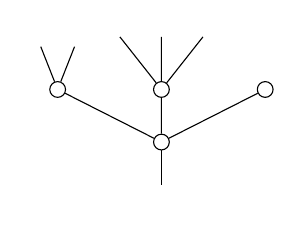
\begin{tikzpicture}[grow=up, every node/.style = {font=\footnotesize},level distance = 1.9em]%
	\tikzstyle{level 2}=[sibling distance=3.75em]%
	\tikzstyle{level 3}=[sibling distance=1.5em]%
		\node {}%
			child{node [dummy] {}%
				child{node [dummy] {}}%
				child{node [dummy] {}%
					child{}%
					child{}%
					child{}%
				}%
				child{node [dummy] {}%
					child{node {} }%
					child{node {} }%
				}%
			};%
	\end{tikzpicture}%
\]%
encodes the operadic composition
\[
	\O(3) \times \O(2) \times \O(3) \times \O(0) \to \O(5)
\]
where the inputs $\O(3), \O(2), \O(3), \O(0)$ correspond to the nodes (i.e. circles) in the tree, with arity given by number of incoming edges (i.e. edges immediately above)
and the output $\O(5)$ has arity given by counting leaves (i.e. edges at the top, not capped by a node).
Similarly, the role of equivariant trees is, in the context of equivariant operads, to encode such operadic compositions together with fixed point compatibilities.  
A detailed introduction to equivariant trees can be found in \cite[\S 4]{Pe17}, where the second author develops the theory of equivariant dendroidal sets (which is a parallel approach to equivariant operads), though here we include only a single representative example.
Let $G = \{ \pm 1, \pm i, \pm j, \pm k\}$ denote the group of quaternionic units 
and $G \geq H \geq K \geq L$ denote the subgroups %
$H = \langle j \rangle$, %
$K = \langle -1 \rangle$, %
$L = \{1\}$.
There is then a $G$-tree $T$ with 
\textit{expanded representation}
given by the two trees on the left below and
\textit{orbital representation}
given by the (single) tree on the right.
\begin{equation}\label{D6SMALLER EQ}
	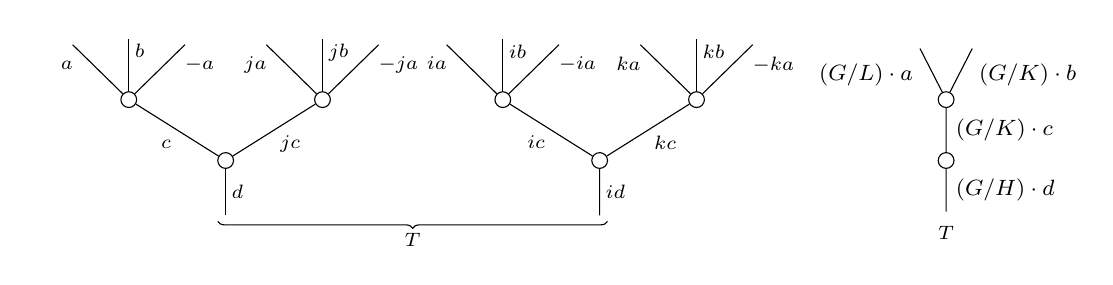
\begin{tikzpicture}[auto,grow=up, level distance = 2.2em,
	every node/.style={font=\scriptsize,inner sep = 2pt}]%
		\tikzstyle{level 2}=[sibling distance=7em]%
		\tikzstyle{level 3}=[sibling distance=2.25em]%
			\node at (4.75,0){}%	
				child{node [dummy] {}%
					child{node [dummy] {}%
						child{node {}%
						edge from parent node [swap,very near end] {$-k a$}}%
						child[level distance = 2.4em]{node {}%
						edge from parent node [swap,near end] {$k b$}}%
						child{node {}%
						edge from parent node [very near end] {$k a$}}%
					edge from parent node [swap] {$k c$}}%
					child{node [dummy] {}%
						child{node {}%
						edge from parent node [swap,very near end] {$-i a$}}%
						child[level distance = 2.4em]{node {}%
						edge from parent node [swap,near end] {$i b$}}%
						child{node {}%
						edge from parent node [very near end] {$i a$}}%
					edge from parent node  {$i c$}}%
				edge from parent node [swap] {$i d$}};%
			\node at (0,0){}%	
				child{node [dummy] {}%
					child{node [dummy] {}%
						child{node {}%
						edge from parent node [swap,very near end] {$-j a$}}%
						child[level distance = 2.4em]{node {}%
						edge from parent node [swap,near end] {$j b$}}%
						child{node {}%
						edge from parent node [very near end] {$j a$}}%
					edge from parent node [swap] {$j c$}}%
					child{node [dummy] {}%
						child{node {}%
						edge from parent node [swap,very near end] {$-a\phantom{j}$}}%
						child[level distance = 2.4em]{node {}%
						edge from parent node [swap,near end] {$b\phantom{j}$}}%
						child{node {}%
						edge from parent node [very near end] {$\phantom{-j}a$}}%
					edge from parent node  {$\phantom{j}c$}}%
				edge from parent node [swap] {$d$}};%
		\begin{scope}[every node/.style={font=\footnotesize}]%
			\node at (9.15,0){}%
				child{node [dummy] {}%
					child{node [dummy] {}%
						child{node {}%
						edge from parent node [swap,very near end] {$(G/K) \cdot b$}}%
						child{node {}%
						edge from parent node [very near end] {$(G/L) \cdot a$}}%
					edge from parent node [right] {$(G/K) \cdot c$}}%
				edge from parent node [right] {$(G/H) \cdot d$}};%
		\end{scope}%
		\draw[decorate,decoration={brace,amplitude=2.5pt}] (4.85,0) -- (-0.1,0) node[midway,inner sep=4pt]{$T$}; %
		\node at (9.15,-0.15) {$T$};
	\end{tikzpicture}%
\end{equation}%
We note that $G$ acts on the expanded representation of $T$ as indicated by the edge labels (so that the edges $a,b,c,d$ have stabilizers $L$, $K$, $K$, $H$ respectively), and the orbital representation is obtained by collapsing the edge orbits of the expanded representation. As explained in \cite[Example 4.9]{Pe17}, $T$ then encodes the fact that for any 
equivariant operad $\O \in \mathsf{Op}^G$ the composition 
$\mathcal{O}(2) \times \mathcal{O}(3)^{\times 2} \to 
\mathcal{O}(6)$ restricts to a fixed point composition
\begin{equation}\label{INTFIXPTCOMP EQ}
\O(H/K)^{H} \times \O(K/L \amalg K/K)^{K} \to
\O(H/L \amalg H/K)^{H}
\end{equation}
where $\O(X)$ for an $H$-set (resp. $K$-set) $X$ denotes $\O(|X|)$ together with a suitably mixed $H$-action ($K$-action).
We note that the inputs 
$\O(H/K)^{H}$, $\O(K/L \amalg K/K)^{K}$ in
(\ref{INTFIXPTCOMP EQ})
correspond to the nodes of the orbital representation
in (\ref{D6SMALLER EQ}), though in contrast to the non-equivariant case arity is now determined by both incoming and outgoing \textit{edge orbits}, while the output 
$\O(H/L \amalg H/K)^{H}$
is similarly determined by both the leaf and root edge orbits.
The existence of maps of the form (\ref{INTFIXPTCOMP EQ}) is essentially tantamount to the subtlest 
closure property for indexing systems $\mathcal{F}$,
self-induction (cf. \cite[Def. 3.20]{BH15}),
and similar tree descriptions exist for all other closure properties, as detailed in 
\cite[\S 9]{Pe17}.

We can now at last give a full informal description of the category $\mathsf{Op}_G$ featured in 
our main result, Theorem \ref{MAINQUILLENEQUIV THM}.
A genuine equivariant operad
$\mathcal{P} \in \mathsf{Op}_G$
has levels $\mathcal{P}(X)$ for each $H$-set $X$, $H\leq G$, 
that mimic the role of the fixed points $\O(X)^H \simeq \O(|X|)^{\Gamma_X}$ for 
$\mathcal{O} \in \mathsf{Op}^G$.
More explicitly, there are restriction maps 
$\mathcal{P}(X) \to \mathcal{P}(X|_{K})$ for $K \leq H$,
isomorphisms
$\mathcal{P}(X)\simeq \mathcal{P}(g X)$
where $gX$ denotes the conjugate $gHg^{-1}$-set,
and composition maps given by
\[
\P(H/K) \times \P(K/L \amalg K/K) \to \P(H/L \amalg H/K)
\]
in the case of the abstraction of (\ref{INTFIXPTCOMP EQ}), and more generally by
%and multiplication maps
%\begin{align*}%\label{FIXEDPOINTMUL EQ}
\begin{equation}\label{GENGENMULT EQ}
\begin{tikzcd}
  \mathcal{P}(H/K_1 \amalg \cdots \amalg H/K_n)
  \times
  \mathcal{P}(K_1 / L_{11} \amalg \cdots \amalg K_1/L_{1 m_1})
  \times \cdots \times
  \mathcal{P}(K_n / L_{n1} \amalg \cdots \amalg K_n / L_{n m_n})
  \arrow[d]
  \\
  % \to & 
  \mathcal{P}(H / L_{11} \amalg \cdots \amalg H/L_{1 m_1}
  \amalg \cdots \amalg
  H / L_{n1} \amalg \cdots \amalg H/L_{n m_n}
  ).
\end{tikzcd}
\end{equation}
%\end{align*}
%generalizing (\ref{INTFIXPTCOMP EQ}) (which corresponds to the case $n=1$, $m_1 = 2$, $L_1 = L$, $L_2 = K$).
Lastly, these composition maps %(\ref{FIXEDPOINTMUL EQ})
must satisfy associativity, unitality, compatibility with restriction maps, and equivariance conditions, as encoded by the theory of $G$-trees. 
Rather than making such compatibilities explicit, however, we will find it preferable for our purposes to simply define genuine equivariant operads intrinsically in terms of $G$-trees.


We end this introduction with an alternative perspective on the role of genuine equivariant operads.
The Elmendorf-Piacenza theorem in 
(\ref{COFADJINT EQ})
is ultimately a strengthening of the basic observation that the homotopy groups
$\pi_n(X)$ of a $G$-space $X$ are coefficient systems rather than just $G$-objects.
Similarly, the generalized 
Elmendorf-Piacenza result \cite[Thm. 3.17]{Ste16}
applied to the category 
$\mathcal{V}=\mathsf{sCat}$
of simplicial categories strengthens 
the observation that 
for a $G$-simplicial category $\C$
the associated homotopy category
$\text{ho}(\mathcal{C})$
is a coefficient system of categories rather than just a $G$-category.
Likewise, Theorem \ref{MAINQUILLENEQUIV THM}
strengthens the (not so basic) observation that for a $G$-simplicial operad $\O$ the associated homotopy operad 
$\text{ho}(\mathcal{O})$
is neither just a $G$-operad nor 
just a coefficient system of operads
but rather the richer algebraic structure that we refer to as a ``genuine equivariant operad''.


%We conclude this introduction with an alternative interpretation of our main result, again inspired by Elmendorf-Piacenza.
%One consequence of their result is that $\pi_0$ (and more generally all homotopy groups $\pi_n$) of a $G$-space 
%is not just $G$-set, but instead can be given the structure of a non-trivial coefficient system, 
%recorded by the fact that the diagram on the left below does \textit{not} commute in general.
%\newcommand\dnc[2][\ncirclearrowleft]{%
%  \arrow[start anchor = center, end anchor = center, draw = none]{#2}[description]{#1}}
%\begin{equation}
%        \label{PI_O_EQ}
%        \begin{tikzcd}
%                \Top^{O_G^{op}} 
%                \arrow[d, "\pi_0"'] 
%                \dnc{dr}
                % \arrow[dr, start anchor=center,end anchor=center,draw=none, "\ncirclearrowleft"] 
%                &
%                \Top^G 
%                \arrow[d, "\pi_0"] 
%                \arrow[l, "\iota_{\**}"'] 
%                &&
%                \Op_G(\Top) 
%                \arrow[d, "\pi_0"']
%                \dnc{dr}
                % \arrow[dr, start anchor=center,end anchor=center,draw=none, "\ncirclearrowleft"] 
%                &
%                \Op^G(\Top)
%                \arrow[d, "\pi_0"]
%                \arrow[l, "\iota_{\**}"'] 
%                \\
%                \Set^{O_G^{op}} 
%                & 
%                \Set^G 
%                \arrow[l, "\iota_{\**}"'] 
%                &&
%                \Op_G(\Set)
%                &
%                \Op^G(\Set)
%                \arrow[l, "\iota_{\**}"'] 
%        \end{tikzcd}
%\end{equation}
%Similarly, the main theorem from \cite{GM13} concerning the model category of $G$-spectra
%%%characterizing the homotopy theory of $G$-spectra,
%%%that the category of $G$-spectra is Quillen equivalent to the category of spectral Mackey functors, 
%homotopically packages the fact that $\pi_0$ of a $G$-spectrum has the further structure of a Mackey functor.

%Analogously, our main result shows that 
%the homotopy operad $\pi_0\O$ associated to a topological $G$-operad 
%$\O \in \Op^G(\Top)$
%is not a coefficient system of (set) operads, but instead has the additional algebraic structure of a non-trivial genuine $G$-operad,
%as again the rightmost diagram in (\ref{PI_O_EQ}) does \textit{not} commute.




\subsection{Main results}

We now discuss our main results.

Fixing a finite group $G$, we
recall that 
$\mathsf{Op}^G(\mathcal{V})
=
\left(\mathsf{Op}(\mathcal{V})\right)^G$
denotes $G$-objects in 
$\mathsf{Op}(\mathcal{V})$.
% \nomenclature[C]{$\V = (\V, \otimes)$}{Symmetric monoidal category}
% \nomenclature[C]{$\O \in \Op^G(\V) = \Op(\V^G)$}{Equivariant Operads in $\V$}
% \nomenclature[C]{$\Sigma = \amalg \Sigma_n$}{Symmetric category}
% \nomenclature[C]{$X \in \Sym^G(\V)  = \Sym(\V^G) = \V^{\Sigma^{op} \times G}$}{Symmetric sequences in $\V$}
% \nomenclature[O]{$H \leq G$}{Finite group and an arbitrary subgroup}
% \nomenclature[O]{$\Lambda \leq \Sigma_m$}{Symmetric group on $m$ letters and an arbitrary subgroup}
% \nomenclature[O]{$\Gamma \leq \Sigma_m$}{Graph subgroup \eqref{GENEOPEQ EQ} of $\Sigma_m$}
% \nomenclature[O]{$\F_n$}{Family of subgroups of $G \times \Sigma_m$ \nomunit{$\F = \set{\F_n}$ collection of families}}
% \nomenclature[C]{$\Op^G_\F(\V)$}{$\F$-model structure \eqref{GENEOPEQMT EQ} on $\Op^G(\V)$}

% \nomenclature[C]{$\mathcal P \in \Op_G(\V)$, $\Op_\F(\V)$}{Genuine equivariant operads in $\V$}
% \nomenclature[C]{$T \in \Omega_G$, $\Omega_\F$}{$G$-trees or $\F$-trees (\S \ref{LRVERT SEC})}
% \nomenclature[C]{$C \in \Sigma_G$, $\Sigma_\F$}{$G$-corollas or $\F$-trees, and quotients (\S \ref{LRVERT SEC})}

% \nomenclature[C]{$\Sym_G(\V) = \V^{\Sigma_G^{op}}$, $\Sym_\F(\V) = \V^{\Sigma_\F^{op}}$}{Genuine symmetric sequences}
% \nomenclature[O]{$\mathbb F$, $\mathbb F_G$}{Free operad and free genuine equivariant operad monads}

% \nomenclature[C]{$\Top$}{Topological spaces}
% \nomenclature[C]{$(\sSet, \times)$, $(\sSet_{\**}, \wedge)$}{Simplicial sets}
COME BACK


\begin{customthm}{I}\label{MAINEXIST1 THM}
Let $(\mathcal{V},\otimes)$
denote either 
$(\mathsf{sSet}, \times)$
or
$(\mathsf{sSet}_{\**}, \wedge)$.

Then there exists a model category structure on 
$\mathsf{Op}^G(\mathcal{V})$ such that 
$\O \to \O'$ is a weak equivalence (resp. fibration)
if all the maps
\begin{equation}\label{GENEOPEQMT EQ}
	\O(n)^{\Gamma} \to \O'(n)^{\Gamma}
\end{equation}
for 
$\Gamma \leq G\times \Sigma_n, \Gamma \cap \Sigma_n = \{\**\}$, 
are weak equivalences (fibrations) in $\mathcal{V}$.

More generally, for $\mathcal{F} = \{\mathcal{F}_n\}_{n \geq 0}$ with $\mathcal{F}_n$ an arbitrary collection of subgroups of $G \times \Sigma_n$ there exists a model category structure on 
$\mathsf{Op}^G(\mathcal{V})$,
which we denote
$\mathsf{Op}^G_{\mathcal{F}}(\mathcal{V})$,
with weak equivalences (resp. fibrations)
determined by (\ref{GENEOPEQMT EQ}) for $\Gamma \in \mathcal{F}_n$.

Lastly, 
analogous 
semi-model category structures
$\mathsf{Op}^G(\mathcal{V})$,
$\mathsf{Op}^G_{\mathcal{F}}(\mathcal{V})$
exist
provided that
$(\mathcal{V},\otimes)$:
\begin{inparaenum}
\item[(i)] is a cofibrantly generated model category;
\item [(ii)] is a closed monoidal model category with cofibrant unit;
\item[(iii)] has cellular fixed points;
\item[(iv)] has cofibrant symmetric pushout powers.
\end{inparaenum}
\end{customthm}

We note that a similar result has also been proven by Guti\'{e}rrez-White in \cite{GW17}.

Theorem \ref{MAINEXIST1 THM}
is proven in \S \ref{MAINEXIST SEC}.
Condition (i) can be found in 
\cite[Def. 2.1.17]{Ho98} while (ii) 
can be found in \cite[Def. 4.2.6]{Ho98}.
The additional conditions (iii) and (iv),
which are less standard, are discussed in 
\S \ref{FAMILY_SEC} and
\S \ref{PUSHPOW SEC}, respectively.
Further, by \textit{semi-model category}
we mean the notion introduced in 
\cite{Ho98} and \cite{Spi01}, 
which relaxes the definition of model structure by requiring that some of the axioms need only apply
if the domains of certain cofibrations are cofibrant. For further details, we recommend the discussion in \cite[\S 2.2]{WY15} or \cite[\S 12.1]{Fre09}.


%The referenced \textit{semi}-model structures 
%are a mild weakening of Quillen model structures, 
%for which half the lifting and factorization axioms only hold for maps with cofibrant source.
%This structure was formally introduced in \cite{Hov98} and \cite{Spi01},
%and has been exploited in, for example,
%\cite{EKMM, Hov98, Spi01, BM03, GH04, Fre09, Whi14, WY15}.
%{\color{blue}
%  Moreover,
%  the introduced weakness will not affect the applications of our results,
%  as, in particular, 
%  the initial operad is cofibrant in our cases of interest,
%  and Reedy semi model structures remain well behaved \cite[Prop. 3]{Spi01}.
%}%COLOR:BLUE
%See \cite[\S 2.2]{WY15} or \cite[\S 12.1]{Fre09} for precise definitions and further discussion.

Our next result concerns the model structure
on the new category 
$\mathsf{Op}_G (\mathcal{V})$ of genuine equivariant operads
introduced in this paper. Before stating the result, we must first outline how 
$\mathsf{Op}_G (\mathcal{V})$
itself is built.
Firstly, the levels of each 
$\mathcal{P} \in \mathsf{Op}_G(\mathcal{V})$,
i.e. the $H$-sets in (\ref{GENGENMULT EQ}),
are encoded by a category $\Sigma_G$ of 
\textit{$G$-corollas}, introduced in \S \ref{LRVERT SEC},
which generalizes the usual category 
$\Sigma$ of finite sets and isomorphisms.
We then define $G$-symmetric sequences by
$\mathsf{Sym}_G(\mathcal{V})=
\mathcal{V}^{\Sigma_G^{op}}$
\index{categories!SymG@$\Sym_G(\mathcal V) = \V^{\Sigma_G^{op}}$}
and,
whenever $\mathcal{V}$ is a closed symmetric monoidal category with diagonals 
(cf. Remark \ref{FINSURJ REM}),
we define in \S \ref{FGMON SEC}
a \textit{free genuine equivariant operad} monad 
$\mathbb{F}_G$ on
\index{monads!FG@$\mathbb F_G$}
$\mathsf{Sym}_G(\mathcal{V})$
whose algebras form the desired category 
$\mathsf{Op}_G(\mathcal{V})$.

Moreover, inspired by the analogues
$\mathsf{Top}^{\mathsf{O}_{\mathcal{F}}^{op}}
	\rightleftarrows 
\mathsf{Top}^G_{\mathcal{F}}$
of the Elmendorf-Piacenza equivalence
where 
$\mathsf{Top}^{\mathsf{O}_{\mathcal{F}}^{op}}$
are partial coefficient systems determined by a family $\mathcal{F}$, 
we show in \S \ref{INDEXING_SECTION}
that (a slight generalization of)
Blumberg-Hill's indexing systems $\mathcal{F}$
give rise to sieves 
$\Sigma_{\mathcal{F}} \hookrightarrow \Sigma_G$
and partial $G$-symmetric sequences
$\mathsf{Sym_{\mathcal{F}}}(\mathcal{F})
=
\mathcal{V}^{\Sigma_{\mathcal{F}}^{op}}$ which are suitably compatible with the monad
$\mathbb{F}_G$,
thus giving rise to categories
$\mathsf{Op}_{\mathcal{F}}(\mathcal{V})$
of \textit{partial genuine equivariant operads}.


\begin{customthm}{II}\label{MAINEXIST2 THM}
Let $(\mathcal{V},\otimes)$
denote either 
$(\mathsf{sSet}, \times)$
or
$(\mathsf{sSet}_{\**}, \wedge)$.
Then the projective model structure on 
$\mathsf{Op}_G(\mathcal{V})$ exists. Explicitly,
a map $\mathcal{P} \to \mathcal{P}'$ is a weak equivalence (resp. fibration) if all maps
\begin{equation}\label{GENEQTHM EQ}
\mathcal{P}(C)
	\to
\mathcal{P}'(C)
\end{equation}
are weak equivalences (fibrations) in $\mathcal{V}$
for each $C \in \Sigma_G$.

More generally, for $\mathcal{F}$ a weak indexing system, the projective model structure on 
$\mathsf{Op}_{\mathcal{F}}(\mathcal{V})$ exists. Explicitly, weak equivalences (resp. fibrations) are
determined by (\ref{GENEQTHM EQ})
for $C \in \Sigma_{\mathcal{F}}$.

Lastly, 
analogous 
semi-model structures on
$\mathsf{Op}_G(\mathcal{V})$,
$\mathsf{Op}_{\mathcal{F}}(\mathcal{V})$
exist
provided that
$(\mathcal{V},\otimes)$:
\begin{inparaenum}
\item[(i)] is a cofibrantly generated model category;
\item [(ii)] is a closed monoidal model category with cofibrant unit;
\item[(iii)] has cellular fixed points;
\item[(iv)] has cofibrant symmetric pushout powers;
\item[(v)] has diagonals.
\end{inparaenum}
\end{customthm}

Theorem \ref{MAINEXIST2 THM} is proven in 
\S \ref{MAINEXIST SEC}
in parallel with Theorem \ref{MAINEXIST1 THM}.
We note that the condition (v) that 
$(\mathcal{V},\otimes)$ has diagonals (cf. Remark \ref{FINSURJ REM}), which is not needed in 
Theorem \ref{MAINEXIST1 THM}, is required to build
the monad $\mathbb F_G$, and hence the categories
$\mathsf{Op}_G(\mathcal{V})$,
$\mathsf{Op}_{\mathcal{F}}(\mathcal{V})$.

The following is our main result.
The explicit formulas for
the functors 
$\iota^{\**},\iota_{\**}$
are found in \eqref{IOTAFUNS EQ}
(also, see Corollaries \ref{TWOADJOINTSOP_COR}
and \ref{TWOADJOINTSOPF COR}).

\begin{customthm}{III}\label{MAINQUILLENEQUIV THM}
Let $(\mathcal{V},\otimes)$
denote either 
$(\mathsf{sSet}, \times)$
or
$(\mathsf{sSet}_{\**}, \wedge)$.

Then the adjunctions, 
where in the more general rightmost case 
$\mathcal{F}$ is a weak indexing system,
\begin{equation}
\begin{tikzcd}[column sep =4em]
	\mathsf{Op}_G(\mathcal{V}) \ar[shift left=1.5]{r}{\iota^{\**}} 
	&
	\mathsf{Op}^G(\mathcal{V})
	\ar[shift left=1.5]{l}{\iota_{\**}},
&
	\mathsf{Op}_{\mathcal F}(\mathcal{V}) 
	\ar[shift left=1.5]{r}{\iota^{\**}} 
	&
	\mathsf{Op}^G_{\mathcal{F}}(\mathcal{V})
	\ar[shift left=1.5]{l}{\iota_{\**}}.
\end{tikzcd}
\end{equation}
are Quillen equivalences.

Morover, 
analogous Quillen equivalences of
semi-model structures\footnote{
See \cite[\S 12.1.8]{Fre09} for a precise definition.}
$\mathsf{Op}_{\mathcal F}(\mathcal{V}) \simeq
\mathsf{Op}^G_{\mathcal{F}}(\mathcal{V})$
exist
provided that
$(\mathcal{V},\otimes)$:
\begin{inparaenum}
\item[(i)] is a cofibrantly generated model category;
\item [(ii)] is a closed monoidal model category with cofibrant unit;
\item[(iii)] has cellular fixed points;
\item[(iv)] has cofibrant symmetric pushout powers;
\item[(v)] has diagonals;
\item[(vi)] has cartesian fixed points.
\end{inparaenum}
\end{customthm}

Theorem \ref{MAINQUILLENEQUIV THM}
is proven in 
\S \ref{MAINTHM_PROOF_SECTION}.
Condition (vi), which is not 
needed in either of
Theorems \ref{MAINEXIST1 THM},\ref{MAINEXIST2 THM}
is discussed in 
\S \ref{PUSHPOW SEC}.


Lastly, our techniques also verify 
the main conjecture of \cite{BH15},
which we discuss in \S \ref{NINFTY_SECTION}.
Moreover, we note that our models for
$N \mathcal{F}$-operads are given by explicit bar constructions.

\begin{customcor}{IV}\label{NINFTY_REAL_COR_MAIN}
For $\V = \sSet$ or $\mathsf{Top}$ and 
$\mathcal{F} = \{\mathcal{F}_n\}_{n \geq 0}$
any weak indexing system,
$N \mathcal{F}$-operads exist. That is, there exist explicit operads $\O$
such that
\begin{equation}\label{NFINFTY2 EQ}
	\O(n)^{\Gamma} \sim 
\begin{cases}
	\** & \text{if } \Gamma \in \mathcal{F}_n
\\
	\emptyset & \text{otherwise}.
\end{cases}
\end{equation}  
In particular, the map $\mathrm{Ho}(N_\infty$-$\Op) \to \mathcal I$
in \cite[Cor. 5.6]{BH15}
 is an equivalence of categories.
 
 Moreover, if $\mathcal{O}'$ has fixed points as in 
 (\ref{NFINFTY2 EQ}) for some collection of graph subgroups 
 $\mathcal{F} = \{\mathcal{F}_n\}_{n \geq 0}$, then 
 $\mathcal{F}$ must be a weak indexing system.
\end{customcor}

%Independently, using different techniques, Rubin \cite{Rub17} and Guti\'{e}rrez-White \cite{GW} have also announced confirmations of this conjecture for (regular) indexing systems.

\subsection{Future Work}

% \nomenclature[C]{$\mathsf{dSet} = \Set^{\Omega^{op}}$, $\mathsf{dSet}^G = \Set^{\Omega^{op} \times G}$}{Dendroidal sets}



In order to simplify our discussion,
this paper focuses exclusively on the theory of 
single colored (genuine) equivariant operads.
Nonetheless, we conjecture that all three of 
Theorems \ref{MAINEXIST1 THM},\ref{MAINEXIST2 THM},\ref{MAINQUILLENEQUIV THM}
extend to the colored setting,
and intend to show this in upcoming work.
We note, however, that an important new subtlety emerges in the 
equivariant setting:
while usual colored equivariant operads have $G$-sets of objects,
colored genuine equivariant operads will instead have \textit{coefficient systems} of objects.

This paper and \cite{Pe17} are the first pieces of a broader project aimed at understanding different models for equivariant operads. 
In the next major step of the project, 
we intend to connect the two papers by
generalizing the main theorem of
Cisinski and Moerdijk in \cite{CM13b} and 
 showing the existence of a Quillen equivalence
\begin{equation}
\begin{tikzcd}[column sep =4em]
	\mathsf{dSet}^G \ar[shift left=1.5]{r} 
	&
	\mathsf{sOp}^G,
	\ar[shift left=1.5]{l}
\end{tikzcd}
\end{equation} 
where $\mathsf{dSet}^G$ is the
category of equivariant dendroidal sets of
\cite{Pe17} and 
$\mathsf{sOp}^G$ the category of equivariant colored simplicial operads with its (conjectural) ``with norms'' model structure,
as discussed in the previous paragraph.




%While this paper focuses soley on \textit{single coloured} operads, 
%we expect the theory to extend immediately to the coloured setting. 
%One key difference is that coloured genuine $G$-operads will have a 
%\textit{coefficient system} of colours: 
%evaluation at a $G$-corolla will include the additional data of 
%a colour for each $G$-orbit of edges, 
%and the isotropy of the colours must match that of its asscoatied edge.
%This feature is inspired by those seen in other models for $G$-operads, on which we now elaborate. 
%More than just for completeness, such an extension will allow for more complete comparisons with the other models for $G$-operads.

%We end this introduction with a brief discussion on the context of this paper. 


%The major goal of the authors' current project is to detail the full story of the homotopy theory of equivariant operads. 
%This paper and \cite{Pe17} form the basis of a generalization of the work of Cisinski-Moerdijk-Weiss, 
%whose work culminates in the square of Quillen-equivalent categories below. 
%%%generalizating the work of, e.g. \cite{Joy01}, \cite{Lu09}, \cite{Bergner}, and Rezk on $\infty$-categories.
%\begin{equation}
%  \label{CM_EQ}
%  \tag{$\filledstar$}
%  \begin{tikzcd}
%    \mathsf{PreOp} 
%    \arrow[d] 
%    & 
%    \mathsf{sOp} 
%    \arrow[l] 
%    \arrow[d, "hcN_d"]
%    \\
%    \mathsf{sdSet} 
%    & 
%    \mathsf{dSet} 
%    \arrow[l]
%  \end{tikzcd}
%\end{equation}
%An additional common feature is the construction of a strict ``homotopy'' category/operad from an $\infty$-category/operad.

%Sequels will extend both of these to the $G$-equivariant context. 
%In particular, we expect the categories $\Op^G_{\mathcal F}(\sSet)$ and $\mathsf{dSet}^G_{\mathcal F}$ to be Quillen equivalent.
%Further, mimicking our alternative interpretation from the end of the introduction,
%multicoloured genuine $G$-operads will provide 
%the natural (and most highly structured) target for the strictification of $G$-$\infty$-operads from \cite{Pe17}. 
%In both cases, we have that 
%the $G$-$\infty$-operads in $\mathsf{dSet}^G$ 
%or the operads in $\Op^G(\Top)$ 
%themselves satisfy a rigid fixed-point condition, 
%but their homotopy operads do \textit{not}.

%Moreover, we note that, as in \cite{Pe17}, there are both 
%multiple possible \textit{categorical} generalizations 
%(i.e. $\mathsf{dSet}^G$ vs. $\mathsf{dSet}_G$, $\Op^G$ vs. $\Op_G$)
%and multiple possible \textit{model categorical} generalizations 
%(i.e $\mathsf{dSet}^G_{\mathcal F}$, $\Op^G_{\mathcal F}$) 
%for each corner of the equivariant version of (\ref{CM_EQ}). 
%Analogous to the main result of this paper, 
%we expect all compatible notions at each corner to be Quillen equivalent 
%(i.e. $\mathsf{dSet}^G_{\mathcal F} \simeq_Q \mathsf{dSet}_{\mathcal F}$). 

%A full exploration of this and the other above topics will be discussed in future papers.
%we will study this precise question, as well as comparisons between the different models.

% \[
% \begin{tikzcd}
%         \Op^G_{\mathcal F}(\V) \arrow[rr, "i_*"] \arrow[dd, shift right, "hcN^G"]& & \Op_G^{\mathcal F}(\V) \arrow[dd, "hcN_G"']\\ \\
%         \mathsf{dSet}^G_{\mathcal F} \arrow[rr, "i_*"'] \arrow[uu, shift left, shift left, dashed, bend left, "Ho^G"] \arrow[uurr, "Ho_G", dashed] && \mathsf{dSet}_G^{\mathcal F} \arrow[uu, shift right, shift right, bend right, dashed, "\mathrm{Ho}_G"']
% \end{tikzcd}
% \]


%We expect that, analogous to the work of Cisinski-Moerdijk, the direct vertical comparisons between $G$-operads and $G$-dendroidal sets will be challenging, hence the need to explore other notions of $G$-$\infty$-operads in the previous paragraph.


\subsection{Outline}

\todo[inline]{when do different pieces of the machine happen?}

This paper is comprised of two major halves, 
with 
\S \ref{PLANAR_SECTION},
\S \ref{GENUINE_OP_MONAD_SECTION}
addressing the definition of the novel structure of
genuine equivariant operads,
and 
\S \ref{FREE_EXTENSIONS_SECTION},
\S \ref{COFIB SEC}
addressing the proofs of the main results,
Theorems \ref{MAINEXIST1 THM},\ref{MAINEXIST2 THM},\ref{MAINQUILLENEQUIV THM}.
A more detailed outline follows.

\S \ref{PRELIM_SECTION}
discusses some preliminary notions and notation that will be used throughout.
Of particular importance are the notions of 
split Grothendieck fibrations,
which we recall in \S \ref{GROTHFIB REF},
and the categorical wreath product defined in 
\S \ref{WREATH SEC}, which we use to define
symmetric monoidal categories with diagonals
(Remark \ref{FINSURJ REM}).

\S \ref{PLANAR_SECTION} lays the groundwork for the definition of genuine equivariant operads in 
\S \ref{GENUINE_OP_MONAD_SECTION} by discussing the concept of node substitution (which is at the core of the definition of free operads)
in the context of equivariant trees. The key idea, which is captured in diagram
(\ref{SUBSDATUMTREES EQ}) and Proposition \ref{SUBSASPULL PROP}
% \ref{SUBDATAUNDERPLAN PROP},\ref{SUBDATAUNDERPLANG COR}, 
is that such substitution data are encoded by special maps of $G$-trees that we call planar tall maps. The bulk of the section is spent studying these types of maps, culminating in the concept of planar strings in \S \ref{PLANARSTRING SEC}, which encode iterated substitution.

\S \ref{GENUINE_OP_MONAD_SECTION} then uses planar strings to provide the formal definition of the category 
$\mathsf{Op}_G(\mathcal{V})$
of genuine equivariant operads in a 
two step process in 
\S \ref{MONSPAN SEC} and \S \ref{FGMON SEC}.
\S \ref{COMPARISON_REGULAR_SECTION} then compares 
the genuine equivariant operad category
$\mathsf{Op}_G(\mathcal{V})$
with the usual equivariant operad category
$\mathsf{Op}^G(\mathcal{V})$,
establishing the necessary adjunction to formulate
Theorem \ref{MAINQUILLENEQUIV THM}.
\S \ref{INDEXING_SECTION}
discusses the notion of partial genuine equivariant operads, which are very closely related to the indexing systems of Blumberg-Hill.


\S \ref{FREE_EXTENSIONS_SECTION} 
proves 
Theorems \ref{MAINEXIST1 THM} and \ref{MAINEXIST2 THM}.
As is often the case when proving existence of projective model structures,
the key to this section is a careful analysis of  the free extensions in $\mathsf{Op}_G$ as in diagram
(\ref{FREE_FG_EXT_EQ}),
with 
\S \ref{LABELSTRI SEC}, 
\S \ref{EXTTREE SEC},
\S \ref{FILTRATION_SECTION}
dedicated to providing a suitable filtration of such free extensions,
and \S \ref{MAINEXIST SEC} concluding the proofs.

\S \ref{COFIB SEC} proves our main result,
Theorem \ref{MAINQUILLENEQUIV THM}.
The core of the technical analysis 
is given in 
\S \ref{FAMILY_SEC},
\S \ref{PUSHPOW SEC}
and \S \ref{G_GRAPH_SECTION}, 
which carefully study the interplay between families of subgroups, fixed points, and pushout products,
and provide the necessary ingredients for
the characterization of the cofibrant objects
in $\mathsf{Op}_G (\mathcal{V})$
given in Lemma \ref{MAINLEM LEM},
and from which 
Theorem \ref{MAINQUILLENEQUIV THM}
easily follows.
\S \ref{NINFTY_SECTION}
then establishes Corollary 
\ref{NINFTY_REAL_COR_MAIN}
by using the theory of genuine equivariant operads
to build explicit cofibrant models for 
$N \mathcal{F}$-operads.

Lastly,
Appendix \ref{TRANSKAN AP}
provides the proof of a lengthy technical result needed when establishing the filtrations in \S \ref{FREE_EXTENSIONS_SECTION}.



%In the first section, we recall background categorical material which will play a role throughout the paper,
%as well as establish notation.
%In Section \ref{PLANAR_SECTION}, 
%we introduce a number of concepts related to $G$-treees, 
%in particular planarity, substitutions, and leaf-root and vertex functors, 
%which are all necessary to build the monad $\mathbb F_G$.
%Further, we use these structures to identify certain pullbacks as categories of strings of maps, 
%which we then use to conveniently package both substitutions and iterations of $\mathbb F_G$.
%After defining the endofunctor $\mathbb F_G$, 
%Section \ref{GENUINE_OP_MONAD_SECTION}
%uses the 
%tools from
%%%results and technical framework of 
%the previous section to both prove $\mathbb F_G$ is in fact a monad and compare it to the usual free operad monad.
%Section \ref{FREE_EXTENSIONS_SECTION} 
%begins our homotopical discussion by 
%analysing and building filtrations of free $\mathbb F_G$-extensions, 
%%%using the realization of the simplicial object in categories of strings of maps,
%%%and building a filtration of such maps.
%through which we prove the main existence results.%, Theorems \ref{MAINEXIST1 THM} and \ref{MAINEXIST2 THM}.
%Finally, in Section \ref{COFIB SEC}
%we investigate the delicate interplay involved when combining cofibrancy between different equivariant categories, 
%yielding the primary argument of our main result, a characterization of cofibrant genuine $G$-operads.
%We end this section, and the paper, by constructing an explicit $N\mathcal F$-operad for any weak indexing system $\mathcal F$.

%We delay the proof of a lengthy result from Section \ref{FREE_EXTENSIONS_SECTION}, 
%which provides the technical backbone to our description of free extensions,
%%%% constructing free extensions using a realization of a simplicial object in categories
%to the appendix.




% \todo[inline]{come back}


% We begin by observing that the free operad $\mathbb{F} X$ generated by a symmetric sequence $X \in \Sym(\V)$, discussed in \cite{Spi01, BM03, Rub17} etc., can be repackaged as a left Kan extension out of $\Omega$.
% \[
% \begin{tikzcd}
%         |[alias=U]| \Omega^{op} \arrow[d, "\mathsf{lr}"'] \arrow[r, "N_X"] & \V & \qquad & |[alias=A]| \Omega_G^{op} \arrow[d, "\mathsf{lr}"'] \arrow[r, "N_Y"] & \V\\
%         \Sigma^{op} \arrow[ur, "\mathbb{F} X"', ""{name=V}] & && \Sigma_G^{op} \arrow[ur, "\mathbb{F}_G Y"', ""{name=B}]
%         \arrow[Rightarrow, from=U, to=V] 
%         \arrow[Rightarrow, from=A, to=B]
% \end{tikzcd}
% \]
% Here, $\mathsf{lr}$ is the ``leaf-root'' or ``valence'' functor, and $N_X$ sends $T$ to $\prod_{v\in V(T)} X(v)$.

% This can be equivariantly generalized, replacing $\Omega$ and $\Sigma$ with $\Omega_G$ and $\Sigma_G$, as seen on the right-hand-side. This yields our ``genuine $G$-operad'' monad $\mathbb{F}_G$, acting on the new category of $G$-sequences $Y\in \Sym_G(\V) = \V^{\Sigma_G^{op}}$. Now, having defined our notion of ``coefficient systems'', we can begin further analysis. As is often the case, we desire a clear understanding of free $\mathbb{F}_G$-extensions (\ref{FREE_FG_EXT_EQ}). 

% First, we produce multiple categorical manipulations of this functor. We modify both $\Omega_G$ and $\mathbb{F}_G$ to construct a description of coproducts of $\mathbb{F}_G$-algebras as a similar looking left Kan extension. Then, we``add in relations'' found in our free $\mathbb{F}_G$-extension by inserting new maps into this modified $\Omega_G$, via a realization of a simplicial category of strings of such maps. Finally, using this description, we can build a filtration of such free extensions.

% Secondly, we consider the homotopical characteristics of $\mathbb{F}_G$, in particular a detailed study of the interactions of cofibrancy with composition. We also compare $\mathbb{F}$ and $\mathbb{F}_G$, categorically and homotopically, in order to display the Quillen equivalence.

% We now give a brief overview of the remaining sections.

% \todo[inline]{come back}

% In \textbf{\hyperref[PRELIM_SECTION]{Section \ref{PRELIM_SECTION}: Preliminaries}} we identify the major categorical constructions we will be using throughout the paper, as well as establish notion and background material.

% \textbf{\hyperref[PLANAR_SECTION]{Section \ref{PLANAR_SECTION}: Planar and tall maps.}} Our machery requires our trees to record an additional structure, namely a planarization. In this section, we define this notion for $G$-trees, and explore the notion of ``substitution'', a second  structure on the class of trees, which many of our constructions employ.

% \textbf{\hyperref[GENUINE_OP_MONAD_SECTION]{Section \ref{GENUINE_OP_MONAD_SECTION}: The genuine equivariant operad monad.}} Defining $\mathbb{F}_G$ as an endofunctor is fairly straightforward, as is defining composition and unit maps. However, showing that this data forms a monad requires a more subtle analysis. We define a more general monad $N$ on the category of weak spans $\mathsf{WSpan}(\Sigma_G, \V)$, and simplify the discussion through the flexibility of this more general category. It is also here that the concept of ``planar strings'' of maps are introduced.

% \textbf{\hyperref[FREE_EXTENSIONS_SECTION]{Section \ref{FREE_EXTENSIONS_SECTION}: Free extensions and the existence of model structures.}} In this section, we develop the technology to produce free $T$-extensions for a particular class of monads $T$, utilizing the realizations of simplicial categories of planar strings. After providing a filtration of such constructions, we prove the existence of variuos model structures on our categories of algebras.

% %\textbf{\hyperref[MODEL_STRUCTURES_SECTION]{Section \ref{MODEL_STRUCTURES_SECTION}: Model structures.}} Using the description of free extensions developed in the previous section, we produce a filtration of free extensions, and exploit this to transfer model structures from the categories of sequences $\Sym^G$ and $\Sym_G$ onto our categories of operads $\Op^G$ and $\Op_G$.

% \textbf{\hyperref[COFIB SEC]{Section \ref{COFIB SEC}: Cofibrancy and Quillen equivalences.}} This section contains the bulk of the homotopical analysis. It is here that we show that weak indexing systems $\mathcal F$ provide sufficient structure so that their associated $\mathcal F$-model structures are well-behaved, in particular proving the desired Quillen equivalences. We end this section, and this paper, by providing two proofs of the $N_\infty$ realization conjecture.

% % \begin{itemize}
% % \item Defining $\mathbb{F}_G$, and rigorously showing it is a monad on $\Sym_G(\V)$ (Section \ref{GENUINE_OP_MONAD_SECTION}).
% % \item Conveniently expressing free $\mathbb{F}_G$-extensions (Section \ref{FREE_EXTENSIONS_SECTION}).
% % \item Analyzing filtrations of free $\mathbb{F}_G$-extensions to build various model structures (Section \ref{MODEL_STRUCTURES_SECTION}).
% % \item Exploring the interplay between grafting of trees and cofibrancy to prove the above model structures are well-behaved (Section \ref{COFIB SEC}).
% % \end{itemize}

% Much of the machinery in Sections \ref{GENUINE_OP_MONAD_SECTION} and \ref{FREE_EXTENSIONS_SECTION} are built in large categorical generality, designed such that the intuitive descriptions of, for example, the free operad monad and operations on forests, are verified with strict categorical rigor; as such, they may be of broader interest.


\section{Preliminaries}
\label{PRELIM_SECTION}

%This section lists some elementary concepts and results that will be used throughout the paper, but may not be entirely standard.

\subsection{Grothendieck fibrations}\label{GROTHFIB REF}

% \nomenclature[M]{$\pi \colon \mathcal E \to \mathcal B$}{Grothendieck fibration (\S \ref{GROTHFIB REF})}

Recall that a functor 
$\pi \colon \mathcal{E} \to \mathcal{B}$
is called a \textit{Grothendieck fibration} \cite[\S 8.1]{Bo94}
if for every arrow 
$f \colon b' \to b$ in $\mathcal{B}$
and $e \in \mathcal{E}$ such that $\pi(e)=b$,
there exists a \emph{cartesian arrow} 
$f^{\**} e \to e$ lifting $f$,
i.e. an arrow such that for any choice of horizontal arrows 
\[
\begin{tikzcd}[row sep=7pt]
	e'' \ar{rr} \ar[dashed]{rd}[swap]{\exists !} & & 
	e
&
	b'' \ar{rr} \ar{rd} & & 
	b
\\
	& f^{\**} e \ar{ru} &
&
	& b' \ar{ru}[swap]{f} &
\end{tikzcd}
\]
for which the rightmost diagram commutes and 
$e'' \to e$ lifts $b'' \to b$,
there exists a unique dashed arrow
$e'' \to f^{\**} e$ lifting $b'' \to b'$ and making the leftmost diagram commute.

In most contexts the cartesian arrows $f^{\**} e \to e$ are assumed to be defined only up to unique isomorphism, 
but in all examples considered in this paper
we will be able to identify preferred choices of cartesian arrows, and we will refer to those preferred choices as \textit{pullbacks}.
Moreover, pullbacks will be compatible with composition and units in the obvious way, i.e. $g^{\**} f^{\**} e = (fg)^{\**}e$ and $id_b^{\**}e=e$.
On a terminological note, 
the data of a Grothendieck fibration together with 
such choices of pullbacks is sometimes called a 
\textit{split fibration}, but we will have no need to distinguish the two concepts outside
of the present discussion.

A map of Grothendieck fibrations (resp. split fibrations) is then a commutative diagram
\begin{equation}
\begin{tikzcd}\label{GROTHFIBMAP EQ}
	\mathcal{E} \ar{rr}{\delta} \ar{rd}[swap]{\pi} &&
	\bar{\mathcal{E}} \ar{dl}{\bar{\pi}}
\\
	& \mathcal{B}
\end{tikzcd}
\end{equation}
such that $\delta$ preserves cartesian arrows (pullbacks).


There is a well known equivalence between Grothendieck fibrations over $\mathcal{B}$ and contravariant pseudo-functors
$\mathcal{B}^{op} \to \mathsf{Cat}$
with split fibrations corresponding to (regular) contravariant functors. We recall how this works in the split case, starting with the covariant version.

\begin{definition}\label{GROTHCONS DEF}
Given a small category $\mathcal{B}$ and functor $\mathcal{E}_{\bullet}$
\begin{equation}
\begin{tikzcd}[row sep = 0em]
	\mathcal{B} \ar{r}{\mathcal{E}_{\bullet}} & \mathsf{Cat} \\
	b \ar[mapsto]{r} & \mathcal{E}_b
\end{tikzcd}
\end{equation}
the \textit{covariant Grothendieck construction}
$\mathcal{B} \ltimes \mathcal{E}_{\bullet}$ (over $\mathcal B$)
has objects pairs $(b,e)$ with $b \in \mathcal{B}$,
$e \in \mathcal{E}_b$ and 
arrows $(b,e) \to (b',e')$ given by pairs
\[(f\colon b \to b', g \colon f_{\**}(e) \to e'),\]
where $f_{\**}\colon \mathcal{E}_b \to \mathcal{E}_{b'}$ is a shorthand for the functor $\mathcal{E}_{\bullet}(f)$.

Note that the chosen pushforward of $(b,e)$ along 
$f \colon b \to b'$ is then $(b',f_{\**} e)$.

Further, for a contravariant functor
$\mathcal{E}_{\bullet} \colon
\mathcal{B}^{op} \to \mathsf{Cat}$,
the \textit{contravariant Grothendieck construction} is
$(\mathcal{B}^{op} \ltimes 
\mathcal{E}_{\bullet}^{op})^{op}$
(over $\mathcal B$).
\end{definition}


One useful property of Grothendieck fibrations is that
right Kan extensions can be computed using fibers, i.e., 
given a functor $F \colon \mathcal{E} \to \mathcal{V}$ into a complete category $\mathcal{V}$ one has
\begin{equation}\label{FIBERKAN EQ}
	\mathsf{Ran}_{\pi}F (b)
\simeq
	\mathsf{lim} F{|_{b \downarrow \mathcal{E}}}
\simeq
	\mathsf{lim} F|_{\mathcal{E}_b}
\end{equation}
where the first identification is the usual pointwise formula for Kan extensions (cf. \cite[X.3 Thm. 1]{McL})
and the second identification follows by noting that due to the existence of cartesian arrows the fibers
$\mathcal{E}_b$ are initial (in the sense of \cite[IX.3]{McL})
in the undercategories $b \downarrow \mathcal{E}$.
In fact, a little more is true: a choice of cartesian arrows 
yields a right adjoint to the inclusion
$\mathcal{E}_b \hookrightarrow b \downarrow \mathcal{E}$, so that $\mathcal{E}_b$ is a coreflexive subcategory of 
$b \downarrow \mathcal{E}$,
a well known sufficient condition for initiality.
In practice, we will also need a generalization of the Kan extension formula (\ref{FIBERKAN EQ}) for maps of Grothendieck fibrations as in (\ref{GROTHFIBMAP EQ}).
Keeping the notation therein, given an $\bar{e} \in \bar{\mathcal{E}}$ we will write 
$\bar{e} \downarrow_{\pi} \mathcal{E} \hookrightarrow
\bar{e} \downarrow \mathcal{E}$
for the full subcategory of those pairs 
$\left(e,f \colon \bar{e} \to \delta(e)\right)$
such that $\bar{\pi}(f) = id_{\bar{\pi}(\bar{e})}$.


\begin{proposition}\label{FIBERKANMAP PROP}
	Given a map of Grothendieck fibrations
	as in \eqref{GROTHFIBMAP EQ},
	each subcategory $\bar{e} \downarrow_{\pi} \mathcal{E}$
	for $\bar{e} \in \bar{\mathcal{E}}$
	is an initial subcategory of $\bar{e} \downarrow \mathcal{E}$
	and hence for each functor 
	$\mathcal{E} \to \mathcal{V}$
	with $\mathcal{V}$ complete one has
\begin{equation}\label{FIBERKANMAP EQ}
	\mathsf{Ran}_{\delta}F (\bar{e})
\simeq
	\mathsf{lim} F{|_{\bar{e} \downarrow \mathcal{E}}}
\simeq
	\mathsf{lim} F|_{\bar{e} \downarrow_{\pi} \mathcal{E}}.
\end{equation}	
\end{proposition}

\begin{proof}
One readily checks that the assignment
$
	(e,f\colon\bar{e} \to \delta(e))
\mapsto
	\left(
	(\pi(f)^{\**}e, \bar{e} \to \delta \pi(f)^{\**}(e))
	\right)
$
(where $\delta \pi(f)^{\**} = \bar{\pi}^{\**}(f) \delta$) is  right adjoint to the inclusion
$\bar{e} \downarrow_{\pi} \mathcal{E} \hookrightarrow
\bar{e} \downarrow \mathcal{E}$, so that the claim follows by coreflexivity 
(note that if we are not in the split case, pullbacks may be chosen arbitrarily).
\end{proof}

%\begin{proof}
%  We must show that the appropriate iterated overcategories are non-empty and connected. To that end, suppose we have a map $\phi: d\to f(c)$ in $\mathcal D$, and let $q := r(\phi): r(d) \to r(c)$. Since $\mathcal C$ is fibrant over $\mathcal E$, we have a Cartesian arrow $q': c' \to c$ lifting $q: r(d) = r(c') \to r(c)$. Thus we have diagrams in $\mathcal E$ and $\mathcal D$ of the form
%\[
%\begin{tikzcd}
%  r(d) \arrow[dr, "r(\phi)"'] \arrow[r, equal, "id"] & r(c') \arrow[d, "q"] &\qquad \qquad & d \arrow[dr, "\phi"'] \arrow[r, dashed, "\exists!"] & f(c') \arrow[d, "f(q')"] \\
%  & r(c) & & & f(c)
%\end{tikzcd}
%\]
%As $f$ preserves Cartesian arrows, $f(q')$ is Cartesian, and hence we have a unique lifting $p(\phi): d \to f(c')$ of $r(d) = r(c')$. Thus the iterated overcategory is inhabited.

%To show it is connected, given any other factorization $d \xrightarrow{\psi} f(c'') \to f(c)$ such that $r(\psi) = id$, we can again use the fact that $q'$ is Cartesian to produce a lift $f(c'') \to f(c')$ of $r(c'') = r(c')$; by uniqueness of the map $d \to f(c')$, we have that the diagram below commutes, finishing the proof.
%\[
%\begin{tikzcd}
%  & d \arrow[dl, "\exists!"'] \arrow[dr, "\psi"] & \\
%  f(c') \arrow[dr, "f(q')"']  && f(c'') \arrow[ll, dashed, %"\exists!"'] \arrow[dl]\\
%  & f(c)
%\end{tikzcd}
%\]
%\end{proof}


We also record the following, the proof of which is straightforward.

\begin{proposition}\label{GROTHSTAB PROP}
	Suppose that $\mathcal{E} \to \mathcal{B}$ is a (split) Grothendieck fibration. Then so is the map of functor categories 
	$\mathcal{E}^{\mathcal{C}} \to \mathcal{B}^{\mathcal{C}}$ for any category $\mathcal{C}$,
        as well as the map 
	$\bar{\mathcal{E}} \to \bar{\mathcal{B}}$ in any pullback of categories
        \[
              \begin{tikzcd}
                    \bar{\mathcal{E}} \ar{r} \ar{d} & \mathcal{E} \ar{d}
                    \\
                    \bar{\mathcal{B}} \ar{r} & \mathcal{B}.
              \end{tikzcd}
        \]	
\end{proposition}




\subsection{Wreath product over finite sets}
\label{WREATH SEC}

Throughout we will let $\Fin$ denote the usual skeleton of the category of (ordered) finite sets and all set maps. Explicitly, its objects are the finite sets $\{1,2,\cdots,n\}$ for $n\geq 0$.


\begin{definition}
	For a category $\C$, we write 
	$\Fin \wr \C = (\Fin^{op} \ltimes (\C^{op})^{\times \bullet})^{op}$ 
	for the contravariant Grothendieck construction (cf. Definition \ref{GROTHCONS DEF}) of the functor
\[
\begin{tikzcd}[row sep=0pt]
	\Fin^{op} \ar{r} & \mathsf{Cat}
\\
	I \ar[r,mapsto] & \C^{\times I}
\end{tikzcd}	
 \]
Explicitly, the objects of $\Fin \wr \C$ are tuples $(c_i)_{i \in I}$ and a map 
$(c_i)_{i \in I} \to (d_j)_{j \in J}$ consists of a pair 
\[(\phi \colon I \to J, (f_i\colon c_i \to d_{\phi(i)})_{i\in I}),\]
 henceforth abbreviated as $(\phi,(f_i))$.
\end{definition}


\begin{remark}\label{WREATHFIXED REM}
Let $(c_i)_{i \in I} \in \Fin \wr \mathcal{C}$
and write $\lambda$ for the partition 
$I = \lambda_1 \amalg \cdots \amalg \lambda_k$
such that $1 \leq i_1, i_2 \leq n$ are in the same class iff
$c_{i_1}, c_{i_2} \in \mathcal{C}$ are isomorphic.
 Writing 
 $\Sigma_{\lambda} = \Sigma_{\lambda_1} \times \cdots \times
 \Sigma_{\lambda_k}$
and picking representatives $i_j \in \lambda_j$,
the automorphism group of  
$(c_i)_{i \in I}$ is given by
\begin{equation}
	\mathsf{Aut}\left( (c_i)_{i \in I} \right)
\simeq
	\Sigma_{\lambda} \wr \prod_{i} \mathsf{Aut}(c_i)
\simeq
	\Sigma_{|\lambda_1|} \wr 
	\mathsf{Aut}(c_{i_1})
		\times \cdots \times	
	\Sigma_{|\lambda_k|} \wr 
	\mathsf{Aut}(c_{i_k}).
\end{equation}
\end{remark}

 
\begin{notation}
      \label{FIN_COA_COS_NOT}
Using the coproduct functor $\Fin^{\wr 2} = \Fin^{\wr \{{0,1\}}} =\Fin \wr \Fin \xrightarrow{\amalg} \Fin$ (where $\coprod_{i\in I} J_i$ is ordered lexicographically) and the singleton $\{1\} \in \Fin$
one can regard the collection of categories 
$\Fin^{\wr n+1 }\wr \C = \Fin^{\wr \{0,\cdots,n\}} \wr \C $ for $n \geq -1$
 as a coaugmented cosimplicial object in $\mathsf{Cat}$.
As such, we will denote by
\[
	\delta^i\colon \Fin^{\wr n } \wr \C \to \Fin^{n+1} \wr \C, \qquad 0 \leq i \leq n
\]
the cofaces obtained by inserting singletons $\{1\} \in \Fin$ and by 
\[
	\sigma^i \colon \Fin^{n+2} \wr \C \to \Fin^{n+1} \wr \C, \qquad 0 \leq i \leq n
\]
the codegeneracies obtained by applying the coproduct 
$\Fin^{\wr 2} \xrightarrow{\amalg} \Fin$ to adjacent 
$\Fin$ coordinates.

Further, note that there are identifications
$\Fin \wr \delta^{i} = \delta^{i+1}$, 
$\Fin \wr \sigma^{i} = \sigma^{i+1}$.
\end{notation}
 

\begin{remark}
	If $\mathcal{V}$ has all finite coproducts then injections and fold maps assemble into a functor as on the left below.
Dually, if $\mathcal{V}$ has all finite products then projections and diagonals assemble into a functor as on the right.
\begin{equation}\label{WREATHPROD EQ}
\begin{tikzcd}[row sep=0pt]
	\Fin \wr \mathcal{V} \ar{r}{\coprod} & \mathcal{V} & &
	(\Fin \wr \mathcal{V}^{op})^{op} \ar{r}{\prod} & \mathcal{V}
\\
	(v_i)_{i \in I} \ar[mapsto]{r} & \coprod_{i \in I}{v_i} & &
	(v_i)_{i \in I} \ar[mapsto]{r} & \prod_{i \in I}{v_i}
\end{tikzcd}
\end{equation}
Moreover, these functors satisfy a number of additional coherence conditions.
Firstly, there is a natural isomorphism $\alpha$ as on the left below
\begin{equation}\label{COHER EQ}
\begin{tikzcd}
	\Fin^{\wr 2} \wr \mathcal{V} 
	\ar{r}{\Fin \wr \coprod} \ar{d}[swap]{\sigma^0}&
	\Fin \wr \mathcal{V} \ar{r}{\coprod} &
	|[alias=Vt]|
	\mathcal{V} \ar[equal]{d}
& &
	\mathcal{V} \ar{d}[swap]{\delta^0} \ar[equal]{rd}
\\
	|[alias=FV]|
	\Fin \wr \mathcal{V} \ar{rr}[swap]{\coprod} &&
	\mathcal{V}
& &
	\Fin \wr \mathcal{V} \ar{r}[swap]{\coprod} &
	\mathcal{V}	
\arrow[Leftrightarrow, from=Vt, to=FV,shorten <=0.10cm,shorten >=0.10cm,"\alpha"]
\end{tikzcd}
\end{equation}
that encodes both reparenthesizing of coproducts and removal of initial objects 
(note that the empty tuple $()_{i \in \emptyset}\in \Fin \wr \mathcal{V}$ is mapped under $\coprod$ to an initial object of $\mathcal{V}$). Additionally, we are free to assume that the triangle on the right of (\ref{COHER EQ}) strictly commutes, i.e. 
that ``unary coproducts'' of singletons $(v)$ are given simply by $v$ itself.
$\alpha$ is then associative in the sense that the composite natural isomorphisms between the two functors
$\Fin^{\wr 3} \wr \mathcal{V} \to \mathcal{V}$
in the diagrams below coincide.
\begin{equation}\label{COHER2 EQ}
\begin{tikzcd}
	\Fin^{\wr 3} \wr \mathcal{V} \ar{d}[swap]{\sigma^0} 
	\ar{r}{\Fin^{\wr 2} \wr \coprod} \ar{d}[swap]{\sigma^0}&
	\Fin^{\wr 2} \wr \mathcal{V} \ar{r}{\Fin \wr \coprod}
	\ar{d}[swap]{\sigma^0}&
	\Fin \wr \mathcal{V} \ar{r}{\coprod} &
	|[alias=Vtt]|
	\mathcal{V} \ar[equal]{d}
&
	\Fin^{\wr 3} \wr \mathcal{V} \ar{d}[swap]{\sigma^0} 
	\ar{r}{\Fin^{\wr 2} \wr \coprod} &
	\Fin^{\wr 2} \wr \mathcal{V} \ar{r}{\Fin \wr \coprod}&
	|[alias=Vtt2]|
	\Fin \wr \mathcal{V} \ar{r}{\coprod} \ar[equal]{d}&
	\mathcal{V} \ar[equal]{d}
\\
	\Fin^{\wr 2} \wr \mathcal{V} 
	\ar{r}{\Fin \wr \coprod} \ar{d}[swap]{\sigma^1}&
	|[alias=FVt]|
	\Fin \wr \mathcal{V} \ar{rr}{\coprod} &&
	|[alias=Vt]|
	\mathcal{V} \ar[equal]{d}
&
	|[alias=FFV]|	
	\Fin^{\wr 2} \wr \mathcal{V} 
	\ar{rr}{\Fin \wr \coprod} \ar{d}[swap]{\sigma^0}&&
	\Fin \wr \mathcal{V} \ar{r}{\coprod} &
	|[alias=Vt2]|
	\mathcal{V} \ar[equal]{d}
\\
	|[alias=FV]|
	\Fin \wr \mathcal{V} \ar{rrr}[swap]{\coprod} &&&
	\mathcal{V}
&
	|[alias=FV2]|
	\Fin \wr \mathcal{V} \ar{rrr}[swap]{\coprod} &&&
	\mathcal{V}
\arrow[Leftrightarrow, from=Vt, to=FV,shorten <=0.10cm,shorten >=0.10cm,"\alpha"]
\arrow[Leftrightarrow, from=Vtt, to=FVt,shorten <=0.10cm,shorten >=0.10cm,"\alpha"]
\arrow[Leftrightarrow, from=Vt2, to=FV2,shorten <=0.10cm,shorten >=0.10cm,"\alpha"]
\arrow[Leftrightarrow, from=Vtt2, to=FFV, shorten <=0.10cm,shorten >=0.10cm,"\Fin \wr \alpha"]
\end{tikzcd}
\end{equation}
Similarly, $\alpha$ is unital in the sense that both of the following diagrams strictly commute or, more precisely,
the composite natural transformation in either diagram is the identity for the functor 
$\coprod \colon \Fin \wr \mathcal{V} \to \mathcal{V}$.
\begin{equation}\label{COHER3 EQ}
\begin{tikzcd}
	\Fin \wr \mathcal{V} \ar{d}[swap]{\delta^0} \ar{r}{\coprod}&
	\mathcal{V} \ar{d}[swap]{\delta^0} \ar[equal]{r}&
	\mathcal{V} \ar[equal]{d}
& &
	\Fin \wr \mathcal{V} \ar{d}[swap]{\delta^1} \ar[equal]{r}&
	\Fin \wr \mathcal{V}\ar[equal]{d} \ar{r}{\coprod}&
	\mathcal{V} \ar[equal]{d}
\\
	\Fin^{\wr 2} \wr \mathcal{V} 
	\ar{r}{\Fin \wr \coprod} \ar{d}[swap]{\sigma^0}&
	\Fin \wr \mathcal{V} \ar{r}{\coprod} &
	|[alias=Vt]|
	\mathcal{V} \ar[equal]{d}
& &
	\Fin^{\wr 2} \wr \mathcal{V} 
	\ar{r}{\Fin \wr \coprod} \ar{d}[swap]{\sigma^0}&
	\Fin \wr \mathcal{V} \ar{r}{\coprod} &
	|[alias=Vt2]|
	\mathcal{V} \ar[equal]{d}
\\
	|[alias=FV]|
	\Fin \wr \mathcal{V} \ar{rr}[swap]{\coprod} &&
	\mathcal{V}
& &
	|[alias=FV2]|
	\Fin \wr \mathcal{V} \ar{rr}[swap]{\coprod} &&
	\mathcal{V}
\arrow[Leftrightarrow, from=Vt, to=FV,shorten <=0.10cm,shorten >=0.10cm,"\alpha"]
\arrow[Leftrightarrow, from=Vt2, to=FV2,shorten <=0.10cm,shorten >=0.10cm,"\alpha"]
\end{tikzcd}
\end{equation}
\end{remark}

\begin{remark}
\label{SIGMA_WR_REM}
More generally, if $\mathcal{V}$ is an arbitrary
symmetric monoidal category, one always has a functor 
$\Sigma \wr \mathcal{V} \xrightarrow{\otimes} \mathcal{V}$
(where as usual $\Sigma \hookrightarrow \Fin$ denotes the skeleton of finite sets and isomorphisms) satisfying the obvious analogues of
(\ref{COHER EQ}), (\ref{COHER2 EQ}), (\ref{COHER3 EQ}),
as is readily shown using the standard coherence results for symmetric monoidal categories 
(moreover, we note that $\alpha$ itself encodes all associativity, unital and symmetry isomorphisms, with the 
right side of (\ref{COHER EQ}) and (\ref{COHER3 EQ})
being mere common sense desiderata for ``unary products'').

It is likely no surprise that the converse is also true, i.e. 
that a functor 
$\Sigma \wr \mathcal{V} \xrightarrow{\otimes} \mathcal{V}$
satisfying the analogues of 
(\ref{COHER EQ}), (\ref{COHER2 EQ}), (\ref{COHER3 EQ})
endows $\mathcal{V}$ with a symmetric monoidal structure.
We will however have no direct need to use this fact, and as such include only a few pointers concerning the associativity pentagon axiom (the hardest condition to check) that the interested reader may find useful. 
Firstly, it becomes convenient to write expressions such as
$(A \otimes B) \otimes C$ instead as 
$(A \otimes B) \otimes (C)$, so as to encode notationally the fact that this is the image of 
$((A,B),(C)) \in \Sigma^{\wr 2} \wr \mathcal{V}$ under the top map in (\ref{COHER EQ}). The associativity isomorphisms are hence given by the composites
$
(A \otimes B) \otimes (C) \xrightarrow{\simeq} 
A \otimes B \otimes C \xleftarrow{\simeq}
(A) \otimes (B \otimes C)
$
obtained by combining 
$\alpha_{((A,B),(C))}$ 
and
$\alpha_{((A),(B,C))}$.
The pentagon axiom is then checked by combining \textit{six} instances of each of the squares in (\ref{COHER2 EQ}) (i.e. twelve squares total), most of which are obvious except for the fact that the $(A\otimes B) \otimes (C \otimes D)$ vertex of the pentagon contributes two pairs of squares rather than just one, with each pair corresponding to the two alternate expressions 
$((A \otimes B)) \otimes ((C) \otimes (D))$ and 
$((A) \otimes (B)) \otimes ((C \otimes D))$.
\end{remark}

%Given 
%$\mathsf{Fin} \wr \mathcal{V} \to \mathcal{V}$ with suitable isomorphisms $\alpha$, we define the associators by
%\[
%\begin{tikzcd}
%	(A \cdot B) \cdot (C) \ar{r}{\alpha} &
%	A \cdot B \cdot C &
%	(A) \cdot (B \cdot C) \ar{l}[swap]{\alpha}
%\end{tikzcd}
%\]
%and the unit morphisms by
%\[
%\begin{tikzcd}
%	(A) \cdot () \ar{r}{\alpha} &
%	A &
%	() \cdot (A) \ar{r}{\alpha} &
%	A
%\end{tikzcd}
%\]

%The associativity ``pentagon'' axiom follows from
%\[
%\begin{tikzcd}[column sep=5pt]
%	&
%	((A \cdot B)) \cdot ((C) \cdot (D)) 
%	\ar[equal]{r}{\mathsf{F} \wr \alpha} \ar{ld}[swap]{\alpha} &
%	(A \cdot B) \cdot (C \cdot D) \ar{dd} &
%	((A) \cdot (B)) \cdot ((C \cdot D)) 
%	\ar[equal]{l}[swap]{\mathsf{F} \wr \alpha} \ar{rd}{\alpha}
%\\
%	(A \cdot B) \cdot (C) \cdot (D) \ar{rrd} & 
%	&
%	&
%	&
%	(A) \cdot (B) \cdot (C \cdot D)\ar{lld}
%\\
%	((A \cdot B) \cdot (C)) \cdot ((D)) \ar{u}{\alpha}
%	\ar{d}[swap]{\mathsf{F} \wr \alpha}& 
%	&
%	A \cdot B \cdot C \cdot D
%	&
%	&
%	((A)) \cdot ((B) \cdot (C \cdot D)) \ar{u}[swap]{\alpha} \ar{d}{\mathsf{F} \wr \alpha}
%\\
%	(A \cdot B \cdot C) \cdot (D) \ar{rru} &
%	&
%	&
%	&
%	(A) \cdot (B \cdot C \cdot D) \ar{llu}
%\\
%	&
%	((A) \cdot (B \cdot C))\cdot ((D)) \ar{r}[swap]{\alpha} \ar{lu}{\mathsf{F} \wr \alpha} &
%	(A) \cdot (B \cdot C) \cdot (D) \ar{uu} &
%	((A)) \cdot ((B \cdot C) \cdot (D)) \ar{l}{\alpha} 
%	\ar{ru}[swap]{\mathsf{F} \wr \alpha}
%\end{tikzcd}
%\]

%The identity axiom is

%\[
%\begin{tikzcd}
%	((A) \cdot ()) \cdot ((B)) \ar{r}{\alpha} \ar{d}[swap]{\mathsf{Fin} \wr \alpha} &
%	(A) \cdot () \cdot (B) \ar{d} &
%	((A)) \cdot (() \cdot (B)) \ar{l}[swap]{\alpha}
%	\ar{d}{\mathsf{Fin} \wr \alpha}
%\\
%	(A) \cdot (B) \ar[equal]{r}&
%	A \cdot B &
%	(A) \cdot (B) \ar[equal]{l}
%\end{tikzcd}
%\]

%The symmetry morphism is defined in the obvious way as 
%$\otimes (\tau)$ for $\tau$ the 
%isomorphism
%$(A,B) \simeq (B,A)$ in $\Sigma_2 \wr \mathcal{V}$.

%The inverse law is then simply automatic and the coherence of symmetry with unit is naturality of $\alpha$, as in the diagram
%\[
%\begin{tikzcd}
%	(A) \cdot () \ar{r}{\tau} \ar{d}{\alpha} &
%	() \cdot (A) \ar{d}{\alpha}
%\\
%	A \ar{r}[swap]{\tau} &
%	A
%\end{tikzcd}
%\]

%Lastly, associativity coherence is then ensured by the diagram (where the center triangle commutes since it is in the image of $\Sigma_3 \wr \mathcal{V}$)
%\[
%\begin{tikzcd}[column sep = 5pt]
%	&
%	&
%	(A)\cdot (B \cdot C) \ar{rr}{\tau} \ar{dl}[swap]{\alpha}&
%	&
%	(A) \cdot (C \cdot B)\ar{dr}{\alpha}
%\\
%	&
%	A \cdot B  \cdot C \ar{rrrr}{\tau} \ar{ddrr}[swap]{\tau}&
%	&
%	& 
%	&
%	A \cdot C \cdot B \ar{ddll}{\tau}
%\\
%	(A \cdot B) \cdot (C) \ar{ru}{\alpha} \ar{rd}[swap]{\tau}&
%	&
%	&
%	&
%	&
%	&
%	(A \cdot C)  \cdot (B) \ar{lu}[swap]{\alpha} \ar{dl}{\tau}
%\\
%	&
%	(B\cdot A) \cdot (C) \ar{rr}[swap]{\alpha} &&
%	B \cdot A \cdot C &&
%	(B) \cdot (A \cdot C)	\ar{ll}{\alpha}
%\end{tikzcd}
%\]


\begin{remark}\label{FINSURJ REM}
	In lieu of the two previous remarks,
	and writing $\Fin_s \hookrightarrow \Fin$ 
	for the subcategory of surjections,
	we define a 
	\textit{symmetric monoidal category with fold maps}
	as a category $\mathcal{V}$ together with a functor
	$\Fin_s \wr \mathcal{V} \xrightarrow{\otimes} \mathcal{V}$
	satisfying the analogues of  
	(\ref{COHER EQ}), (\ref{COHER2 EQ}), (\ref{COHER3 EQ}).
	Further, the dual of such $\mathcal{V}$ is called a 
	\textit{symmetric monoidal category with diagonals}\footnote{
	These have also been called \textit{relevant monoidal categories} \cite{DP07}.}.
	
	Similarly, replacing $\Fin_s$ with the subcategory
$\Fin_i \hookrightarrow \Fin$ of injections yields the notion of a \textit{symmetric monoidal category with injection maps} or, dually, \textit{symmetric monoidal category with projections}\footnote{
These are equivalent to \textit{semicartesian symmetric monoidal categories} \cite{Lei16}.}.

Finally, we note that if a symmetric monoidal category has both diagonals and projections, it must in fact be \textit{cartesian monoidal} \cite[IV.2]{EK66}.
\end{remark}


\begin{remark}
	Extending Notation \ref{FIN_COA_COS_NOT} one sees that 
	$\Fin \wr (\minus)$, 
	$\Fin_i \wr (\minus)$,
	$\Fin_s \wr (\minus)$,
	$\Sigma \wr (\minus)$
define monads in the category of categories.
%	
%      As analogues of Notation (\ref{FIN_COA_COS_NOT}) also hold when replacing $\Fin$ with
%      $\Sigma = \Fin_{iso}$, $\mathsf{F}_s$, $\mathsf{F}_i$, and their duals,
%      we have that every one of these $\F_{\**} \wr (-)$ is a monad on the category of categories,
%      the free symmetric monoidal category with the appropriate additional structure specified by the above remarks.
      %/(co)cartesian monoidal category (with folds/diagonals/injections/projections)
\end{remark}


We end this section by collecting some straightforward lemmas
that will be used in \S \ref{GENUINE_OP_MONAD_SECTION}.

\begin{lemma}\label{FWRGROTH LEM}
	If $\mathcal{E} \to \mathcal{B}$ a (split) Grothendieck fibration then so is 
	$\Fin_s \wr \mathcal{E} \to \Fin_s \wr \mathcal{B}$.

	Moreover, if 
	$\mathcal{E} \to \bar{\mathcal{E}}$ is a map of (split) Grothendieck fibrations over $\mathcal{B}$ then
	$\Fin_s \wr \mathcal{E} \to \Fin_s \wr \bar{\mathcal{E}}$ is a map of (split) Grothendieck fibrations over $\Fin_s \wr \mathcal{B}$.
\end{lemma}

\begin{proof}
Given a map 
$(\phi,(f_i)) \colon
(b'_i)_{i \in I} \to (b_j)_{j \in J}$ 
in $\Fin \wr \mathcal{B}$
and object $(e_j)_{j \in J}$ one readily checks that its pullback can be defined by $(f^{\**}_{\phi(i)}e_{\phi(i)})_{i \in I}$.
\end{proof}


\begin{lemma}\label{FINWREATPRODLIM LEM}
Suppose that $\mathcal{V}$ is a bicomplete monoidal category with fold maps such that
the monoidal product %coproducts
commutes with limits in each variable. If the leftmost diagram
\begin{equation}\label{WRRAN EQ}
	\begin{tikzcd}[column sep = 3.5em]
	\mathcal{C} \ar{r}[swap,name=F]{}{G} \ar{d}[swap]{k} &
	\mathcal{V} & 
	& 
	\Fin_s \wr \mathcal{C} \ar{r}[swap,name=FF]{}{\Fin_s \wr G} \ar{d}[swap]{\Fin_s \wr k}&
	\Fin_s \wr \mathcal{V} \ar{r}{\otimes} &
	\mathcal{V}
		\\
	|[alias=D]|\mathcal{D} \ar{ru}[swap]{H} &
	& & 
	|[alias=FD]|\Fin_s \wr \mathcal{D} \ar{ru}[swap]{\Fin_s \wr H}
	\ar[bend right=13]{rru}[swap]{\otimes \circ \Fin_s \wr H}
	\arrow[Rightarrow, from=D, to=F,shorten <=0.10cm,"\eta"]
	\arrow[Rightarrow, from=FD, to=FF,shorten <=0.10cm,"\Fin_s \wr \eta"]
	\end{tikzcd}
\end{equation}
is a right Kan extension diagram then so is the composite of the rightmost diagram. 

Dually, if $\mathcal{V}$ has diagonals,
the monoidal product %products
commutes with colimits in each variable, and the leftmost diagram
\begin{equation}\label{WRLAN EQ}
	\begin{tikzcd}[column sep = 4.5em]
	\mathcal{C}^{op} \ar{r}[swap,name=F]{}{G} \ar{d}[swap]{k^{op}} & 
	\mathcal{V} & 
	(\Fin_s \wr \mathcal{C})^{op} \ar{d}[swap]{(\Fin_s \wr k)^{op}} 
	\ar{r}[swap,name=FF]{}{(\Fin_s \wr G^{op})^{op}} & 
	(\Fin_s \wr \mathcal{V}^{op})^{op} \ar{r}{\otimes} &
	\mathcal{V}
\\
	|[alias=D]|\mathcal{D}^{op} \ar{ru}[swap]{H} &
	& 
	|[alias=FD]|(\Fin_s \wr \mathcal{D})^{op} 
	\ar{ru}[swap]{(\Fin_s \wr H^{op})^{op}}
	\ar[bend right=13]{rru}[swap]{\otimes \circ (\Fin_s \wr H^{op})^{op}}
	&
	\arrow[Leftarrow, from=D, to=F,shorten <=0.10cm,"\epsilon"]
	\arrow[Leftarrow, from=FD, to=FF,shorten <=0.10cm]
	\end{tikzcd}
\end{equation}
is a left Kan extension diagram then so is the composite of the rightmost diagram. 
\end{lemma}


\begin{proof}
	Unpacking definitions using the pointwise formula for Kan extensions (cf. \cite[X.3 Thm. 1]{McL} or \eqref{FIBERKAN EQ}), the claim concerning (\ref{WRRAN EQ}) amounts to showing that for each $(d_i) \in \Fin_s \wr \mathcal{D}$ one has natural isomorphisms
	\begin{equation}\label{POINTKAN EQ}
	\underset{((d_i) \to (kc_j))\in
	\left( (d_i) \downarrow \Fin_s \wr \C \right) }{\lim} {\left(\bigotimes_j{G(c_j)}\right)}
		\simeq	
	\bigotimes_i \underset{(d_i  \to kc_i) \in d_i \downarrow \C}{\lim}
	\left(G(c_i)\right).
	\end{equation}
Proposition \ref{FIBERKANMAP PROP} now applies to 
the map $\Fin_s \wr \mathcal{C} \to \Fin_s \wr \mathcal{D}$ of Grothendieck fibrations over $\Fin_s$ and one readily checks that
$(d_i)\downarrow_{\pi} \Fin_s \wr \mathcal{C} \simeq
\prod_{i}{(d_i\downarrow \mathcal{C})}
$
so that 
	\[
	\underset{((d_i) \to (kc_j))\in
	\left( (d_i)\downarrow \Fin_s \wr \C \right) }{\lim} {\left(\bigotimes_j{G(c_j)}\right)}
		\simeq	
	\underset{(d_i \to kc_i)\in
	\prod_{i} \left( {d_i \downarrow \mathcal{D}} \right)}{\lim}
	\left(\bigotimes_i{G(c_i)}\right)
	\]
and the isomorphisms (\ref{POINTKAN EQ}) now follow from the assumption that the monoidal product commutes with limits in each variable.
\end{proof}

\begin{remark}
      The previous results also hold if we replace $\Fin_s$ with $\Fin$, $\Fin_i$, $\Sigma$.
      %, and appropriately update the requirements on $(\mathcal V, \otimes)$.
\end{remark}

\subsection{Monads and adjunctions}

%Whenever possible and by default, all depictions of adjunctions $\mathcal C \rightleftarrows \mathcal D$ will have the right adjoint on the bottom.

In \S 4 we will make use of the following straightforward results concerning the transfer of monads along adjunctions
(note that $L$ (resp. $R$) denotes the left (right) adjoint).


\begin{proposition}\label{MONADADJ1 PROP}
Let
$
L \colon \mathcal{C} \rightleftarrows \mathcal{D} \colon R
$
be an adjunction and $T$ a monad on $\mathcal{D}$.
Then:
\begin{itemize}
\item[(i)] $RTL$ is a monad and $R$ induces a functor
$R \colon \mathsf{Alg}_T(\mathcal{D}) \to \mathsf{Alg}_{RTL}(\mathcal{C})$;
\item[(ii)] if $LRTL \xrightarrow{\epsilon} TL$ is an isomorphism one further has an induced adjunction
\[
L \colon \mathsf{Alg}_{RTL}(\mathcal{C})
	\rightleftarrows
\mathsf{Alg}_{T}(\mathcal{D}) \colon R.
\]
\end{itemize}
\end{proposition}


\begin{proposition}\label{MONADADJ PROP}
Let
$
L \colon \mathcal{C} \rightleftarrows \mathcal{D} \colon R
$
be an adjunction, $T$ a monad on $\mathcal{C}$, and suppose further that
\[
	LR \xrightarrow{\epsilon} id_{\mathcal{D}}, 
\qquad
	LT \xrightarrow{\eta} LTRL
\]
are natural isomorphisms 
(so that in particular $\mathcal{D}$ is a reflexive subcategory of $\mathcal{C}$).
Then:
\begin{itemize}
\item[(i)] $LTR$ is a monad, with multiplication and unit given by
\[LTRLTR \xrightarrow{\eta^{-1}} LTTR \to LTR,\qquad
id_{\mathcal{D}} \xrightarrow{\epsilon^{-1}} LR \to LTR;
\]
\item[(ii)]
$d \in \mathcal{D}$ is a $LTR$-algebra iff $Rd$ is a $T$-algebra;
\item[(iii)] there is an induced adjunction
\[
L \colon \mathsf{Alg}_{T}(\mathcal{C})
	\rightleftarrows
\mathsf{Alg}_{LTR}(\mathcal{D}) \colon R.
\]
\end{itemize}
\end{proposition}



Any monad $T$ on $\C$ induces obvious monads $T^{\times l}$ on $\C^{\times l}$.
More generally, and 
letting $I$ denote the identity monad,
a partition 
$\{1,\cdots,l\} = \lambda_a \amalg \lambda_i$,
which we denote by $\lambda$,
determines a monad 
$T^{\times \lambda} = T^{\times \lambda_a} \times I^{\times \lambda_i}$ on $\mathcal{C}^{\times l}$.
Here ``$a$'' stands for ``active'' and ``$i$'' for ``inert''.

Such monads satisfy a number of compatibility conditions. 
Firstly, if $\lambda'_a \subseteq \lambda_a$
there is a monad map
$T^{\times \lambda'} \Rightarrow T^{\times \lambda}$,
and we write $\lambda' \leq \lambda$.
Moreover, writing $\alpha^{\**} \colon 
\C^{\times m} \to \C^{\times l}$
for the forgetful functor induced by
a map $\alpha \colon \{1,\cdots,l\} \to \{1,\cdots,m\}$,
one has an equality
$T^{\times \alpha^{\**}\lambda} \alpha^{\**} =
\alpha^{\**} T^{\times \lambda}$,
where $\alpha^{\**}\lambda$ is the pullback partition.
The following is straightforward.

\begin{proposition}\label{MONADICFUN PROP}
	Suppose $\C$ has finite coproducts and write
	$\alpha_{!} \colon \mathcal{C}^{\times l} \to 
	\mathcal{C}^{\times m}$
	for the left adjoint of $\alpha^{\**}$. 
	Then the map
\begin{equation}\label{MONADFUNCTORALPHA EQ}
	T^{\times \alpha^{\**} \lambda} \Rightarrow \alpha^{\**} T^{\times \lambda} \alpha_{!}
\end{equation}
adjoint to the identity 
$T^{\times \alpha^{\**}\lambda} \alpha^{\**} =
\alpha^{\**} T^{\times \lambda}$
is a map of monads on $\C^{\times l}$.

Hence, since $T^{\times \lambda} \alpha_!$ is a right 
$\alpha^{\**} T^{\times \lambda}\alpha_{!}$-module, 
it is also a right $T^{\times \lambda'}$-module\footnote{
Recall that a right (resp. left) module
over a monad $T$ on $\mathcal{C}$
is a functor $M \colon \mathcal{C} \to \mathcal{D}$
(resp. $N \colon \mathcal{D} \to \mathcal{C}$)
together with an action natural transformation
$M \circ T \Rightarrow M$
(resp. $T \circ N \Rightarrow N$)
that is suitably associative and unital.}
whenever
$\lambda' \leq \alpha^{\**} \lambda$.
Finally, the natural map 
\begin{equation}\label{MONADFUNCTORALPHADOU EQ}
	\alpha_{!} T^{\times \alpha^{\**} \lambda} \Rightarrow  T^{\times \lambda} \alpha_{!}
\end{equation}
is a map of right $T^{\times \alpha^{\**} \lambda}$-modules, 
and thus also a map of right 
$T^{\times \lambda'}$-modules
whenever $\lambda' \leq \alpha^{\**} \lambda$.
\end{proposition}

%\begin{proof}
%We first note that 
%$(FG)^{\times \lambda} = F^{\times \lambda} G^{\times \lambda}$.

%Letting $\eta, \epsilon$ denote the unit and counit for the 
%$(\alpha_{!},\alpha^{\**})$ adjunction, 
%(\ref{MONADFUNCTORALPHA EQ})
%is then the composite
%\[
%	T^{\times \alpha^{\**} \lambda} \xrightarrow{\eta} 
%	T^{\times \alpha^{\**} \lambda} \alpha^{\**} \alpha_{!}  %=
%	\alpha^{\**} T^{\times \lambda}\alpha_{!}.
%\]
%That this is a monad map is the condition that the following multiplication and unit diagrams commute.
%\[
%\begin{tikzcd}
%	T^{\times \alpha^{\**} \lambda} \circ T^{\times \alpha^{\**} \lambda} \ar{d} \ar{r} &
%	\alpha^{\**} T^{\times \lambda} \alpha_{!} \circ 
%	\alpha^{\**} T^{\times \lambda} \alpha_{!} \ar{d} &
%	I^{\times n} \ar{d} \ar{rd}& 	
%\\
%	T^{\times \alpha^{\**} \lambda} \ar{r} &
%	\alpha^{\**} T^{\times \lambda} \alpha_{!} &
%	T^{\times \alpha^{\**} \lambda} \ar{r} &
%	\alpha^{\**} T^{\times \lambda} \alpha_{!}
%\end{tikzcd}
%\]
%We argue only the case of the leftmost multiplication diagram, with commutativity of the unit diagram following by a similar but simpler argument. Since precomposition
%$(\minus) \circ \alpha^{\**}$
%is left adjoint to precomposition
%$(\minus) \circ \alpha_{!}$
%this follows from the following commutative diagram.
%\[
%\begin{tikzcd}[column sep=1.5em]
%	T^{\times \alpha^{\**} \lambda}  T^{\times \alpha^{\**} \lambda}  \alpha^{*} \ar[equal]{r} \ar{dd}&
%	T^{\times \alpha^{\**} \lambda}  \alpha^{*}  T^{\times \lambda} \ar{r}{\eta}
%	\ar[equal]{rd} &
%	T^{\times \alpha^{\**} \lambda} \alpha^{\**} \alpha_{!} \alpha^{*} T^{\times \lambda} \ar{d}{\epsilon} \ar[equal]{r}&
%	\alpha^{\**} T^{\times \lambda} \alpha_{!} \alpha^{\**}  T^{\times \lambda} \ar{d}{\epsilon}
%\\
%	& &
%	T^{\times \alpha^{\**} \lambda}  \alpha^{*}  T^{\times \lambda} \ar[equal]{r} &
%	\alpha^{*}  T^{\times \lambda}  T^{\times \lambda} \ar{d}
%\\
%	T^{\times \alpha^{\**} \lambda}  \alpha^{*} \ar[equal]{rrr} &&&
%	\alpha^{*} T^{\times \lambda}
%\end{tikzcd}
%\]
%\end{proof}

\begin{remark}\label{PRECOMPPOSTCOMP REM}
We unpack the content of (\ref{MONADFUNCTORALPHADOU EQ}) when 
$\alpha \colon \{1,\cdots,l\} \to \**$ is the unique map to the singleton $\**$, in which case we write $\alpha_{!} = \coprod$.
We thus have commutative diagrams
\begin{equation}\label{RIGHTMODULETMAPAUX EQ}
\begin{tikzcd}
	\coprod_{j \in \lambda_a} TT A_j \amalg \coprod_{j \in \lambda_i} A_j
	\ar{r} \ar{d} &
	T\left( \coprod_{j \in \lambda_a} T A_j \amalg \coprod_{j \in \lambda_i} A_j \right) \ar{d}
\\
	\coprod_{j \in \lambda_a} T A_j \amalg \coprod_{j \in \lambda_i} A_j
	\ar{r} &
		T\left( \coprod_{j \in \lambda_a} A_j \amalg \coprod_{j \in \lambda_i} A_j \right)
\end{tikzcd}
\end{equation}
for each collection $\left( A_j \right)_{j\in\underline{l}}$ in $\mathcal{C}$,
where the vertical maps
come from the right $T^{\times \lambda}$-module structure.
Writing $\mathbin{\check{\amalg}}$ for the coproduct of $T$-algebras and recalling the canonical identifications 
$\mathbin{\check{\coprod}}_{k \in K} (T A_k) \simeq T
\left( \coprod_{k \in K} A_k \right)$, 
(\ref{RIGHTMODULETMAPAUX EQ}) shows that the 
right $T^{\times \lambda}$-module structure on $T \circ \coprod$
codifies the multiplication maps
\[
\mathbin{\check{\coprod}}_{j \in \lambda_a} TT A_j 
	\mathbin{\check{\amalg}} 
\mathbin{\check{\coprod}}_{j \in \lambda_i} T A_j
	\to
\mathbin{\check{\coprod}}_{j \in \lambda_a} T A_j 
	\mathbin{\check{\amalg}}  
\mathbin{\check{\coprod}}_{j \in \lambda_i} T A_j.
\] 
\end{remark}






\section{Planar and tall maps, and substitution}\label{PLANAR_SECTION}


Throughout, we will assume that the reader is familiar with the category $\Omega$ of trees.
%While not hard to correctly guess the objects of $\Omega$, the exact definition of the arrows can be more surprising.
A good introduction to $\Omega$ is given by 
\cite[\S 3]{MW07}, where arrows are described both via 
the ``colored operad generated by a tree''  and by identifying explicit generating arrows, called faces and degeneracies.
Alternatively, $\Omega$ can also be described 
using the algebraic model of 
\textit{broad posets}
introduced by Weiss in \cite{We12} and further worked out by the second author in \cite[\S 5]{Pe17}.
This latter will be our ``official'' model,
though a detailed understanding of broad posets is needed only
to follow our formal discussion of planar structures in \S \ref{PLASTR SEC}.
Otherwise, the reader willing to accept the results of \S \ref{PLASTR SEC} should 
need only an intuitive grasp of the notations 
$\underline{e} \leq e$,
$f \leq_d e$ and $e^{\uparrow}$
to read the remainder of the paper.
Such understanding can be obtained from 
\cite[Example 5.10]{Pe17}
and Example \ref{PLANAREX EX} below.


Given a finite group $G$, there is also a category $\Omega_G$
of $G$-trees, jointly discovered by the authors and first discussed by the second author in 
\cite[\S 4.3,\S 5.3]{Pe17}, which we now recall.
Firstly, we let $\Phi$ denote the category of forests, i.e.
``formal coproducts of trees''.
A broad poset description of $\Phi$ is found in \cite[\S 5.2]{Pe17},
but here we prefer the alternative definition $\Phi = \Fin \wr \Omega$.
The category of $G$-forests is then 
$\Phi^G$, i.e. the category of $G$-objects in $\Phi$. 
Similarly writing
$\Fin^G$ for the category of $G$-objects in $\Fin$ and
identifying the $G$-orbit category as the subcategory
$\mathsf{O}_G \hookrightarrow \Fin^G$
of those sets with transitive actions, $\Omega_G$ can be described as given by the pullback of categories
\begin{equation}\label{OGDEF EQ}
\begin{tikzcd}
	\Omega_G \ar{r} \ar{d}[swap]{\mathsf{r}} & 
	\Phi^G \arrow{d}{\mathsf{r}}
\\
	\mathsf{O}_G \ar{r} & \Fin^G
\end{tikzcd}
\end{equation}
(where $\mathsf{r}: \Phi \to \Fin$ is the \emph{root functor},
sending a forest to its set of roots),
which is a repackaging of \cite[Def. 5.44]{Pe17}.
Explicitly, a $G$-tree $T$ is then a tuple 
$T = (T_x)_{x \in X}$ with $X \in \mathsf{O}_G$
together with isomorphisms
$T_x \to T_{g x}$ that are suitably associative and unital.



\subsection{Planar structures}\label{PLASTR SEC}



The specific model for the orbit category $\mathsf{O}_G$
used in (\ref{OGDEF EQ}) has extra structure not found in the usual model (i.e. that of the $G$-sets $G/H$ for $H \leq G$),
namely the fact that each $X \in \mathsf{O}_G$
comes with a canonical total order 
(the underlying set of $X$ being one of the sets $\{1,\cdots,n\}$).

We will find it convenient to use a model of $\Omega$ with similar extra structure, given by planar structures on trees.
Intuitively, a planar structure on a tree is the data of a planar representation of the tree, and 
definitions of \textit{planar trees} along those lines
are found throughout the literature.
However, to allow for precise proofs of some key results 
concerning the interaction of planar structures with the maps in $\Omega$ 
(namely Propositions \ref{PLANARPULL PROP},  \ref{SUBDATAUNDERPLAN PROP})
we will instead use a combinatorial definition 
of planar structures in the context of broad posets.

In what follows a tree will be a 
\textit{dendroidally ordered broad poset}
as in \cite{We12}, \cite[Def. 5.9]{Pe17}.


\begin{definition}\label{PLANARIZE DEF}
	Let $T \in \Omega$ be a tree. A \textit{planar structure} of $T$ is an extension of the descendancy partial order $\leq_d$ to a total order $\leq_p$ such that: 
	\begin{itemize}
		\item \textit{Planar}: if $e \leq_p f$ and $e \nleq_d f$ then 
		$g \leq_d f$ implies $e \leq_p g$.
	\end{itemize} 
\end{definition}

{\color{red} HERE}


\begin{example}\label{PLANAREX EX}
An example of a planar structure on a tree $T$ follows, with $\leq_p$ encoded by the hexadecimal number labels
(so that $9<a<b<c<d$).
\[
	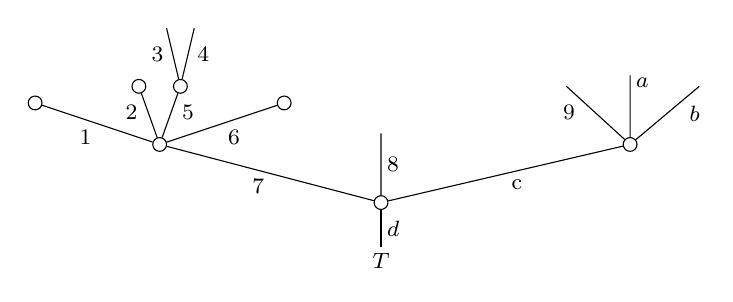
\begin{tikzpicture}[grow=up,auto,level distance=2.1em,
	every node/.style = {font=\footnotesize,inner sep=2pt},
	dummy/.style={circle,draw,inner sep=0pt,minimum size=1.75mm}]
		\node at (0,0) {$T$}
			child{node [dummy] {}
				child[sibling distance = 9em]{node [dummy] {}
					child[sibling distance = 2.5em]{
					edge from parent node [near end,swap] {$b$}}
					child[level distance=2.5em]{
					edge from parent node [very near end,swap] {$a$}}				
					child[sibling distance = 2.3em]{
					edge from parent node [near end] {$9$}}
				edge from parent node [swap] {c}}
				child[level distance =2.5em]{
				edge from parent node [swap] {$8$}}
				child[sibling distance = 8em]{node [dummy] {}
					child[sibling distance =3em, level distance = 1.5 em]{node [dummy] {}
					edge from parent node [swap] {$6$}}
					child[sibling distance = 1.5em]{node [dummy] {}
						child[sibling distance =1em]{
						edge from parent node [swap,near end] {$4$}}
						child[sibling distance =1em]{
						edge from parent node [near end] {$3$}}
					edge from parent node [very near end,swap] {$5$}}
					child[sibling distance =1.5em]{node [dummy] {}
					edge from parent node [very near end] {$2$}}
					child[sibling distance =3em,level distance =1.5em]{node [dummy] {}
					edge from parent node {$1$}}
				edge from parent node {$7$}}
			edge from parent node [swap] {$d$}};
	\end{tikzpicture}
\]
Intuitively, given a planar depiction of a tree $T$, $e \leq_d f$ holds when the downward path from $e$ passes through $f$.
For example, $3 \leq_d 7$ but $7 \not \leq_d 9$.
On the other hand, $e \leq_p f$ holds if either
$e \leq_d f$ or if the downward path from $e$ is to the left of the downward path from $f$ (as measured at the node where the paths intersect).

For $\underline{e}$ a tuple of edges and $e$ an edge,
we write $\underline{e} \leq e$
if there is a subtree diagram with leaf tuple 
$\underline{e}$ and root $e$.
For example, one has 
$789ab \leq d$,
$34 \leq 7$, 
$2346 \leq 7$.

For each edge $e$ topped by a vertex, the notation $e^{\uparrow}$ denotes the tuple of edges immediately above $e$.
In our example, 
$d^{\uparrow} = 78c$,
$7^{\uparrow} = 1256$,
$2^{\uparrow} = \epsilon$ 
(where $\epsilon$ is the empty tuple),
and $9^{\uparrow}$ is undefined.
The vertex above $e$ is then encoded by the \emph{broad relation}
$e^{\uparrow} \leq e$.
\end{example}

{\color{red} HERE}

It is visually clear that a planar depiction of a tree amounts to choosing a total order for each of the sets of \textit{input edges} of each node (i.e. those edges immediately above that node).

While we will not need to make this last statement precise, we will nonetheless find it convenient to show that our Definition \ref{PLANARIZE DEF} of planarity is equivalent to such choices of total orders for each of the sets of input edges.
To do so, we first introduce some notation.


\begin{notation}\label{INPUTPATH NOT}
	Let $T \in \Omega$ be a tree and $e \in T$ an edge. We will denote
	\[ I(e) =\{f \in T \colon e \leq_d f \} \]
and refer to this poset as the \textit{input path of $e$}.
\end{notation}

We will repeatedly use the following, which is a consequence of \cite[Cor. 5.26]{Pe17}.

\begin{lemma}\label{INCOMPNOTOP}
If $e \leq_d f$, $e \leq_d f'$, then $f,f'$ are $\leq_d$-comparable. 
\end{lemma}


\begin{proposition}\label{INPUTPATHS PROP}
	Let $T \in \Omega$ be a tree. Then
	\begin{itemize}
		\item[(a)] for any $e \in T$ the finite poset $I(e)$ is totally ordered;
		\item[(b)] the poset $(T,\leq_d)$ has all joins, denoted $\vee$. In fact, $\bigvee_{i} e_i = \min (\bigcap_{i} I(e_i))$.
	\end{itemize}
\end{proposition}

\begin{proof}
	(a) is immediate from Lemma \ref{INCOMPNOTOP}.
        To prove (b) we note that
        the root edge is in every input path, hence
	$\min (\bigcap_{i} I(e_i))$ exists by (a), and that this is clearly the join $\bigvee_i {e_i}$.
\end{proof}


\begin{notation}
	Let $T \in \Omega$ be a tree and suppose that $e <_d b$. We will denote by $b^{\uparrow}_e \in T$ the predecessor of $b$ in $I(e)$.
\end{notation}


\begin{proposition}\label{INPUTPREDECESSORPROP PROP}
Suppose $e,f$ are $\leq_d$-incomparable edges of $T$ and write $b= e \vee f$. Then
\begin{itemize}
\item [(a)] $e <_d b$, $f<_d b$ and $b^{\uparrow}_e \neq b^{\uparrow}_f$;
\item [(b)] $b^{\uparrow}_e, b^{\uparrow}_f \in b^{\uparrow}$. In fact $\{b^{\uparrow}_e\} = I(e) \cap b^{\uparrow}$,
$\{b^{\uparrow}_f\} = I(f) \cap b^{\uparrow}$;
\item[(c)] if $e' \leq_d e$, $f' \leq_d f$ then 
$b = e' \vee f'$ and $b^{\uparrow}_{e'} = b^{\uparrow}_{e}$, $b^{\uparrow}_{f'} = b^{\uparrow}_{f}$.
\end{itemize}
\end{proposition}


\begin{proof}
(a) is immediate: the condition $e = b$ (resp. $f = b$) would imply $f \leq_d e$ (resp. $e \leq_d f$)
while the condition $b^{\uparrow}_e = b^{\uparrow}_f$ would provide a predecessor of $b$ in $I(e) \cap I(f)$. 

For (b), note that any relation $a <_d b$ factors as 
$a \leq_d b^{\star}_a <_d b$ for some unique $b^{\**}_a \in b^{\uparrow}$, where uniqueness follows from Lemma \ref{INCOMPNOTOP}. Choosing $a=e$ implies $I(e) \cap b^{\uparrow} = \{b^{\**}_e\}$ and letting $a$ range over edges such that $e \leq_d a <_d b$ shows that $b^{\**}_e$ is in fact the predecessor of $b$.

To prove (c) one reduces to the case $e'=e$, in which case it suffices to check $I(e) \cap I(f') = I(e) \cap I(f)$. But if it were otherwise there would exist an edge $a$ satisfying
$f' \leq_d a <_d f$ and $e \leq_d a$, and this would imply $e \leq_d f$, contradicting our hypothesis.
\end{proof}


\begin{proposition}
\label{TERNARYJOIN PROP}
Let $c = e_1 \vee e_2 \vee e_3$.
Then $c = e_i \vee e_j$ iff $c^{\uparrow}_{e_i} \neq c^{\uparrow}_{e_j}$.

Therefore, all ternary joins in $(T,\leq_d)$ are binary, i.e.
\begin{equation}\label{TERNJOIN EQ}
	c = e_1 \vee e_2 \vee e_3 = e_i \vee e_j
\end{equation}
for some $1\leq i <j \leq 3$, and
(\ref{TERNJOIN EQ}) fails for 
 at most one choice of $1\leq i <j \leq 3$.
\end{proposition}


\begin{proof}
If $c^{\uparrow}_{e_i} \neq c^{\uparrow}_{e_j}$ then
$c = \min\left(I(e_i) \cap I(e_j)\right) = e_i \vee e_j$, whereas the converse follows from Proposition \ref{INPUTPREDECESSORPROP PROP}(a).

The ``therefore'' part follows by noting that 
$c^{\uparrow}_{e_1}$, $c^{\uparrow}_{e_2}$, $c^{\uparrow}_{e_3}$
can not all coincide, or else $c$ would not be the minimum of
$I(e_1) \cap I(e_2) \cap I(e_3)$. 
\end{proof}


\begin{example} In the following example $b = e \vee f$, $c = e \vee f \vee g$, $c^{\uparrow}_e= c^{\uparrow}_f =b$.
\[
	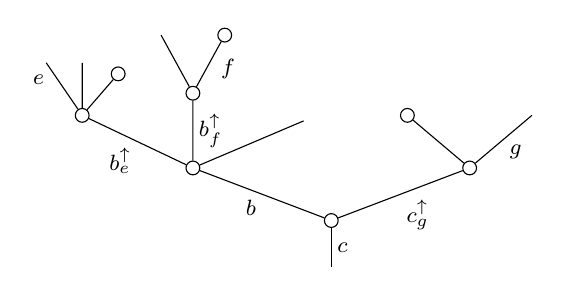
\begin{tikzpicture}[grow=up,auto,level distance=1.9em,
	every node/.style = {font=\footnotesize,inner sep=2pt},
	dummy/.style={circle,draw,inner sep=0pt,minimum size=1.75mm}]
		\node at (0,0) {}
			child{node [dummy] {}
				child[sibling distance = 10em]{node [dummy] {}
					child[sibling distance = 4.5em]{
					edge from parent node [swap] {$g$}}
					child[sibling distance = 4.5em]{node [dummy] {}}
				edge from parent node [swap] {$c_g^{\uparrow}$}}
				child[sibling distance = 10em]{node [dummy] {}
					child[sibling distance = 4em,level distance=1.7em]
					child[sibling distance = 1.5em,level distance=2.7em]{node [dummy] {}
						child[level distance=2.1em,sibling distance = 2.3em]{node [dummy] {}
						edge from parent node [near end,swap] {$f$}}		
						child[level distance=2.1em,sibling distance = 2.3em]{
						edge from parent node [near end] {}}
					edge from parent node [swap] {$b^{\uparrow}_{f}$}}
					child[sibling distance = 4em]{node [dummy] {}
						child[sibling distance =1.3em, level distance = 1.5 em]{node [dummy]  {}
						edge from parent node [swap] {}}
						child[sibling distance = 1.3em]{
						edge from parent node [very near end,swap] {}}
						child[sibling distance =1.3em]{
						edge from parent node [very near end] {$e$}}
					edge from parent node {$b^{\uparrow}_e$}}
				edge from parent node {$b$}}
			edge from parent node [swap] {$c$}};
	\end{tikzpicture}
\]
\end{example}


Given a set $S$ of size $n$ we write
$\textsf{Ord}(S) \simeq \mathsf{Iso}(S,\{1,\cdots,n\})$. We will also abuse notation by regarding its objects as pairs $(S,\leq)$ where $\leq$ is a total order on $S$.



\begin{proposition}\label{PLANARIZATIONCHAR PROP}
	Let $T \in \Omega$ be a tree, 
	with $V(T)$ its set of vertices.
	There is a bijection
\[
	\begin{tikzcd}[row sep = 0em]
		\{\text{planar structures }(T,\leq_p)\} \ar{r}{\simeq} &
		\prod_{(a^{\uparrow} \leq a) \in V(T)} \mathsf{Ord}(a^{\uparrow}) \\
		\leq_p \ar[mapsto]{r} & (\leq_p|_{a^{\uparrow}})
	\end{tikzcd}	
\]
\end{proposition}


\begin{proof}
We will keep the notation of Proposition \ref{INPUTPREDECESSORPROP PROP} throughout,
i.e. $e, f$ are $\leq_d$-incomparable edges and we write $b = e \vee f$. 

	We first show injectivity,
	i.e. that the restrictions $\leq_p|_{a^{\uparrow}}$ determine if 
	$e <_p f$ holds or not.
If $b^{\uparrow}_e <_p b^{\uparrow}_f$, the relations
$e \leq_d b^{\uparrow}_e <_p b^{\uparrow}_f \geq_d f$
and Definition \ref{PLANARIZE DEF} imply it must be $e <_p f$.
Dually, if $b^{\uparrow}_f <_p b^{\uparrow}_e$ then 
$f <_p e$. Thus 
$b^{\uparrow}_e <_p b^{\uparrow}_f \Leftrightarrow e <_p f$ and injectivity follows.

To check surjectivity, 
%that (\ref{PLANAR EQ}) is surjective,
 it suffices (recall that $e,f$ are assumed $\leq_d$-incomparable) to check that
defining $e \leq_p f$ to hold iff $b^{\uparrow}_e < b^{\uparrow}_f$ holds in $b^{\uparrow}$ yields a planar structure.

Antisymmetry and the total order conditions are immediate, and it thus remains to check the transitivity and planar conditions.
Transitivity of $\leq_p$ in the case $e' \leq_d e <_p f$ and the planar condition, which is the case $e <_p f \geq_d f'$, follow from Proposition \ref{INPUTPREDECESSORPROP PROP}(c). Transitivity of $\leq_p$ in the case $e <_p f \leq_d f'$
follows since either $e \leq_d f'$ or else $e,f'$ are $\leq_d$-incomparable, in which case one can apply Proposition \ref{INPUTPREDECESSORPROP PROP}(c) with the roles of $f,f'$ reversed.

It remains to check transitivity in the hardest case, that of 
$e <_p f <_p g$ with $\leq_d$-incomparable $f,g$.
We write $c = e \vee f \vee g$.
By the ``therefore'' part of Proposition \ref{TERNARYJOIN PROP}, either:
\begin{inparaenum}
	\item[(i)] $e \vee f <_d c$, in which case 
	Proposition \ref{TERNARYJOIN PROP}
	implies 
	$c=e \vee g$,
	$c^{\uparrow}_e = c^{\uparrow}_f$ and transitivity follows;
	\item[(ii)] $f \vee g <_d c$, which follows just as (i);
	\item[(iii)]  
$e \vee f = f \vee g =c$, in which case 
$c^{\uparrow}_e <
c^{\uparrow}_f <
c^{\uparrow}_g $ in $c^{\uparrow}$
so that $c^{\uparrow}_e \neq c^{\uparrow}_g$ and by Proposition \ref{TERNARYJOIN PROP} it is also 
$c = e \vee g$ and transitivity follows.
\end{inparaenum}
\end{proof}


\begin{remark}\label{CLOSURE REM}
Proposition \ref{PLANARIZATIONCHAR PROP} states in particular that $\leq_p$
is the closure of the $\leq_d$ relations  
and the $\leq_p$ relations within each
$a^{\uparrow}$
under the planar condition in 
Definition \ref{PLANARIZE DEF}.
\end{remark}


The discussion of the substitution procedure in \S \ref{SUBS SEC} 
will be simplified by working with 
a model for the category $\Omega$
with exactly one representative
of each possible planar structure on each tree or, more precisely, a model where the only isomorphisms preserving the planar structure are the identities.
On the other hand, exclusively using such a model for $\Omega$ throughout would, among other issues, make the discussion of faces in \S \ref{OUTTALL SEC} rather awkward.
We now describe our conventions to address such issues.

Let $\Omega^p$ denote the category of \textit{planarized trees},
with objects pairs $T_{\leq_p}=(T,\leq_p)$ of trees together with a planar structure,
and morphisms \textit{underlying} maps of trees (i.e. ignoring the planar structures).
There is a full subcategory $\Omega^s \hookrightarrow \Omega^p$, whose objects we call \textit{standard models}, of those $T_{\leq_p}$ whose underlying set is one of the sets $\underline{n} = \{1,2,\cdots,n\}$ and for which $\leq_p$ coincides with the canonical order.

\begin{example}\label{STANDMODEL EX}
	Some examples of standard models, i.e. objects of $\Omega^s$, follow (further, Example \ref{PLANAREX EX} can also be interpreted as such an example).
\[
	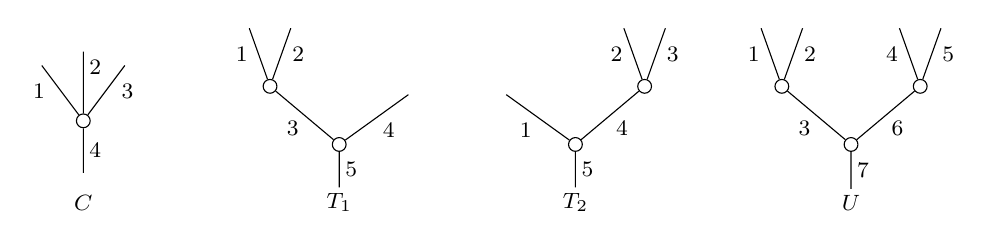
\begin{tikzpicture}[grow=up,auto,level distance=2.1em,
	every node/.style = {font=\footnotesize,inner sep=2pt},
	dummy/.style={circle,draw,inner sep=0pt,minimum size=1.75mm}]
		\node at (-0.25,0) {$C$};
		\node at (-0.25,0.3) {}
			child{node [dummy] {}
				child[sibling distance = 1.5em,level distance= 2em]{
				edge from parent node [swap, near end] {$3$}}
				child[sibling distance = 1.5em,level distance= 2.5em]{
				edge from parent node [swap, near end] {$2$}}
				child[sibling distance = 1.5em,level distance= 2em]{
				edge from parent node [near end] {$1$}}
			edge from parent node [swap] {$4$}};
		\node at (3,0) {$T_1$}
			child{node [dummy] {}
				child[sibling distance = 5em, level distance=1.8em]{
				edge from parent node [swap] {$4$}}
				child[sibling distance = 5em]{node [dummy] {}
					child[sibling distance = 1.5em]{
					edge from parent node [swap,near end] {$2$}}
					child[sibling distance = 1.5em]{
					edge from parent node [near end] {$1$}}
				edge from parent node {$3$}}
			edge from parent node [swap] {$5$}};
		\node at (6,0) {$T_2$}
			child{node [dummy] {}
				child[sibling distance = 5em]{node [dummy] {}
					child[sibling distance = 1.5em]{
					edge from parent node [swap,near end] {$3$}}
					child[sibling distance = 1.5em]{
					edge from parent node [near end] {$2$}}
				edge from parent node [swap] {$4$}}
				child[sibling distance = 5em, level distance=1.8em]{
				edge from parent node {$1$}}
			edge from parent node [swap] {$5$}};
		\node at  (9.5,0) {$U$}
			child{node [dummy] {}
				child[sibling distance = 5em]{node [dummy] {}
					child[sibling distance = 1.5em]{
					edge from parent node [swap,near end] {$5$}}
					child[sibling distance = 1.5em]{
					edge from parent node [near end] {$4$}}
				edge from parent node [swap] {$6$}}
				child[sibling distance = 5em]{node [dummy] {}
					child[sibling distance = 1.5em]{
					edge from parent node [swap,near end] {$2$}}
					child[sibling distance = 1.5em]{
					edge from parent node [near end] {$1$}}
				edge from parent node {$3$}}
			edge from parent node [swap] {$7$}};
	\end{tikzpicture}
\]
Here $T_1$ and $T_2$ are isomorphic to each other but not isomorphic to any other standard model in $\Omega^s$ while both $C$ and $U$ are the unique objects in their isomorphism classes. 
\end{example}

Given $T_{\leq_p} \in \Omega^p$ there is an obvious standard model $T_{\leq_p}^s \in \Omega^s$ given by replacing each edge by its order following $\leq_p$. Indeed, this defines a retraction 
$(\minus)^s \colon \Omega^p \to \Omega^s$
and a natural transformation 
$\sigma \colon id \Rightarrow (\minus)^s$
given by isomorphisms preserving the planar structure
(in fact, the pair $\left((\minus)^s, \sigma \right)$ is  uniquely characterized by this property).


\begin{remark}\label{FORESTPLAN REM}
	Definition \ref{PLANARIZE DEF} readily extends to 
	the broad poset definition of forests $F \in \Phi$ 
	in \cite[Def. 5.27]{Pe17}, with the analogue of
	Proposition \ref{PLANARIZATIONCHAR PROP}
	then stating that a planar structure is 
equivalent to total orderings of the nodes of $F$ together with a total ordering of its set of roots.
There are thus two competing notions of standard forests: the \cite[Def. 5.27]{Pe17} model $\Phi^s$ whose objects are planar forest structures on one of the standard sets $\{1,\cdots,n\}$ and (following the discussion at the start of \S \ref{PLANAR_SECTION})
the model $\Fin \wr \Omega^s$, whose objects are tuples, indexed by a standard set, of planar tree structures on standard sets.
An illustration follows.
\[
	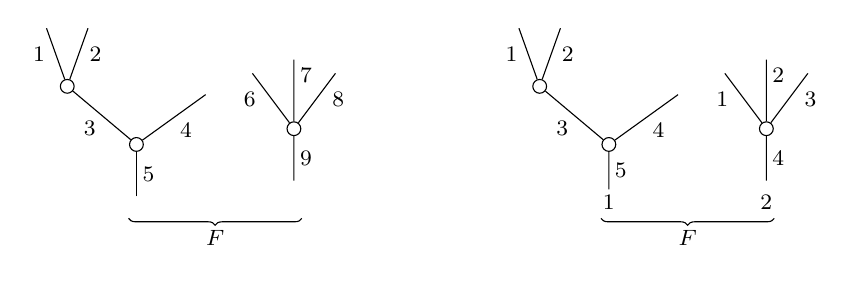
\begin{tikzpicture}[grow=up,auto,level distance=2.1em,
	every node/.style = {font=\footnotesize,inner sep=2pt},
	dummy/.style={circle,draw,inner sep=0pt,minimum size=1.75mm}]
		\node at (2,0.2) {}
			child{node [dummy] {}
				child[sibling distance = 1.5em,level distance= 2em]{
				edge from parent node [swap, near end] {$8$}}
				child[sibling distance = 1.5em,level distance= 2.5em]{
				edge from parent node [swap, near end] {$7$}}
				child[sibling distance = 1.5em,level distance= 2em]{
				edge from parent node [near end] {$6$}}
			edge from parent node [swap] {$9$}};
		\node at (0,0) {}
			child{node [dummy] {}
				child[sibling distance = 5em, level distance=1.8em]{
				edge from parent node [swap] {$4$}}
				child[sibling distance = 5em]{node [dummy] {}
					child[sibling distance = 1.5em]{
					edge from parent node [swap,near end] {$2$}}
					child[sibling distance = 1.5em]{
					edge from parent node [near end] {$1$}}
				edge from parent node {$3$}}
			edge from parent node [swap] {$5$}};
		\node at (8,0) {$2$};
		\node at (8,0.2) {}
			child{node [dummy] {}
				child[sibling distance = 1.5em,level distance= 2em]{
				edge from parent node [swap, near end] {$3$}}
				child[sibling distance = 1.5em,level distance= 2.5em]{
				edge from parent node [swap, near end] {$2$}}
				child[sibling distance = 1.5em,level distance= 2em]{
				edge from parent node [near end] {$1$}}
			edge from parent node [swap] {$4$}};
		\node at (6,0) {$1$}
			child{node [dummy] {}
				child[sibling distance = 5em, level distance=1.8em]{
				edge from parent node [swap] {$4$}}
				child[sibling distance = 5em]{node [dummy] {}
					child[sibling distance = 1.5em]{
					edge from parent node [swap,near end] {$2$}}
					child[sibling distance = 1.5em]{
					edge from parent node [near end] {$1$}}
				edge from parent node {$3$}}
			edge from parent node [swap] {$5$}};
		\draw[decorate,decoration={brace,amplitude=2.5pt}] (2.1,-0.2) -- (-0.1,-0.2) node[midway,inner sep=4pt]{$F$}; %
		\draw[decorate,decoration={brace,amplitude=2.5pt}] (8.1,-0.2) -- (5.9,-0.2) node[midway,inner sep=4pt]{$F$}; %
	\end{tikzpicture}
\]
However, there is a 
\textit{canonical} isomorphism $\Phi^s \simeq \Fin \wr \Omega^s$ 
(with both sides of the diagram above then
depicting the same planar forest). 
Moreover, while the similarly defined categories $\Phi^p$
and $\Fin \wr \Omega^p$ are only equivalent (rather than isomorphic), their retractions onto $\Phi^s \simeq \Fin \wr \Omega^s$ are compatible, and we will thus henceforth not distinguish between 
$\Phi^s$ and $\Fin \wr \Omega^s$.
%Indeed, this follows by either adapting the proof above or by noting that planar structures on $F$ are clearly in bijection with planar structures on the join tree $F \star \eta$ 
%(cf. \cite[Def. 7.44]{Pe17}), which adds a single edge $\eta$ to $F$, serving as the (unique) root of $F \star \eta$.
\end{remark}


\begin{convention}\label{PLANARCONV CON}
      From now on we write simply $\Omega$, $\Omega_G$ to denote the categories $\Omega^s$, $\Omega_G^s$ of standard models (where planar structures are defined in the underlying forest as in Remark \ref{FORESTPLAN REM}). 
      Therefore, whenever a construction produces an object or diagram in $\Omega^p$ or $\Omega^p_G$,
      we always implicitly reinterpret it by using the standardization functor $(\minus)^s$.
      
      Similarly, any finite set (resp. orbital finite $G$-set) together with a total order is implicitly reinterpreted as an object of
      $\Fin$ (resp. $\mathsf{O}_G$).
\end{convention}


\begin{example}
To illustrate our convention, consider the trees in Example \ref{STANDMODEL EX}. 

There are subtrees
$F_1 \subset F_2 \subset U$
where $F_1$ is the subtree with edge set $\{1,2,6,7\}$ and 
$F_2$ is the subtree with edge set $\{1,2,3,6,7\}$, both with inherited tree and planar structures. 
Applying $(\minus)^s$ to the inclusion diagram on the left below then yields a diagram as on the right.
\[
\begin{tikzcd}[row sep = 0.5em,column sep =1.3em]
	F_1 \ar[hookrightarrow]{rr} \ar[hookrightarrow]{rd} & & U & &&
	C \ar{rr} \ar{rd} & & U
\\
	& F_2 \ar[hookrightarrow]{ru} & & &&
	& T_1 \ar{ru}
\end{tikzcd}
\]
Similarly, let $\leq_{(12)}$ and $\leq_{(45)}$ denote alternate planar structures for $U$ exchanging the orders of the pairs $1,2$ and $4,5$, so that one has objects 
$U_{\leq_{(12)}}$, $U_{\leq_{(45)}}$ in $\Omega^p$. 
Applying $(\minus)^s$ to the diagram of underlying identities on the left yields the permutation diagram on the right.
\[
\begin{tikzcd}[row sep = 0.5em,column sep =1.3em]
	U \ar{rr}{id} \ar{rd}[swap]{id} & & U_{\leq_{(45)}} & & &
	U \ar{rr}{(45)} \ar{rd}[swap]{(12)} & & U
\\
	& U_{\leq_{(12)}} \ar{ru}[swap]{id} & & & &
	& U \ar{ru}[swap]{(12)(45)}
\end{tikzcd}
\]
\end{example}


\begin{example}
An additional reason to leave the use of $(\minus)^s$ implicit
as described in Convention \ref{PLANARCONV CON} is that when depicting $G$-trees it is preferable to choose edge labels that describe the action rather than the planarization (which is already implicit anyway).

For example, for the two groups 
$G = \mathbb{Z}_{/4}$ and 
$\bar{G} = \mathbb{Z}_{/3}$, in both diagrams below the orbital representation on the left represents the isomorphism class consisting only of the two trees 
$T_1,T_2 \in \Omega_G$ and
$\bar{T}_1,\bar{T}_2 \in \Omega_{\bar{G}}$
on the right.
\[
	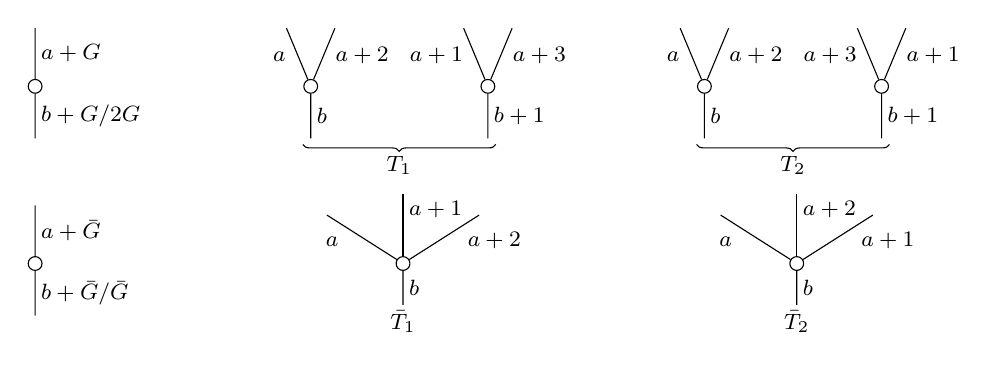
\begin{tikzpicture}[grow=up,auto,level distance=2.1em,
	every node/.style = {font=\footnotesize,inner sep=2pt},
	dummy/.style={circle,draw,inner sep=0pt,minimum size=1.75mm}]
%		\node at (-1,0) {}
%			child{node [dummy] {}
%				child{node [dummy] {}
%					child{
%					edge from parent node [swap] {$a+G$}}
%				edge from parent node [swap] {$b+G/2G$}}
%			edge from parent node [swap] {$c + G/G$}};
%
%		\node at  (3.625,0) {$T_1$}
%			child{node [dummy] {}
%				child[sibling distance = 6em]{node [dummy] {}
%					child[sibling distance = 1.5em]{
%					edge from parent node [swap,near end] {$a+3$}}
%					child[sibling distance = 1.5em]{
%					edge from parent node [near end] {$a+1$}}
%				edge from parent node [swap] {$b+1$}}
%				child[sibling distance = 6em]{node [dummy] {}
%					child[sibling distance = 1.5em]{
%					edge from parent node [swap,near end] {$a+2$}}
%					child[sibling distance = 1.5em]{
%					edge from parent node [near end] {$\phantom{0+}a$}}
%				edge from parent node {$\phantom{1+}b$}}
%			edge from parent node [swap] {$c$}};
%		\node at  (8.625,0) {$T_2$}
%			child{node [dummy] {}
%				child[sibling distance = 6em]{node [dummy] {}
%					child[sibling distance = 1.5em]{
%					edge from parent node [swap,near end] {$a+1$}}
%					child[sibling distance = 1.5em]{
%					edge from parent node [near end] {$a+3$}}
%				edge from parent node [swap] {$b+1$}}
%				child[sibling distance = 6em]{node [dummy] {}
%					child[sibling distance = 1.5em]{
%					edge from parent node [swap,near end] {$a+2$}}
%					child[sibling distance = 1.5em]{
%					edge from parent node [near end] {$\phantom{0+}a$}}
%				edge from parent node {$\phantom{1+}b$}}
%			edge from parent node [swap] {$c$}};
		\node at (-1,-2) {}
			child{node [dummy] {}
				child[sibling distance=1.75em]{
				edge from parent node [swap]  {$a+G$}}
			edge from parent node [swap] {$b+G/2G$}};
		\node at (2.5,-2) {}
			child{node [dummy] {}
				child[sibling distance=1.75em]{
				edge from parent node [swap,near end] {$a+2$}}
				child[sibling distance=1.75em]{
				edge from parent node [near end]  {$\phantom{1+}a$}}
			edge from parent node [swap] {$b$}};
		\node at (4.75,-2) {}
			child{node [dummy] {}
				child[sibling distance=1.75em]{
				edge from parent node [swap,near end] {$a+3$}}
				child[sibling distance=1.75em]{
				edge from parent node [near end]  {$a+1$}}
			edge from parent node [swap] {$b+1$}};
		\draw[decorate,decoration={brace,amplitude=2.5pt}] (4.85,-2) -- (2.4,-2) node[midway,inner sep=4pt]{$T_1$};
		\node at (7.5,-2) {}
			child{node [dummy] {}
				child[sibling distance=1.75em]{
				edge from parent node [swap,near end] {$a+2$}}
				child[sibling distance=1.75em]{
				edge from parent node [near end]  {$\phantom{1+}a$}}
			edge from parent node [swap] {$b$}};
		\node at (9.75,-2) {}
			child{node [dummy] {}
				child[sibling distance=1.75em]{
				edge from parent node [swap,near end] {$a+1$}}
				child[sibling distance=1.75em]{
				edge from parent node [near end]  {$a+3$}}
			edge from parent node [swap] {$b+1$}};
		\draw[decorate,decoration={brace,amplitude=2.5pt}] (9.85,-2) -- (7.4,-2) node[midway,inner sep=4pt]{$T_2$};
		\node at (-1,-4.25) {}
			child{node [dummy] {}
				child[sibling distance=1.75em]{
				edge from parent node [swap]  {$a+\bar{G}$}}
			edge from parent node [swap] {$b+\bar{G}/\bar{G}$}};
		\node at (3.6725,-4.25) {$\bar{T}_1$}
			child{node [dummy] {}
				child[sibling distance = 2.75em,level distance= 1.75em]{
				edge from parent node [swap, near end] {$a+2$}}
				child[sibling distance = 2.75em,level distance= 2.5em]{
				edge from parent node [swap, near end] {$a+1$}}
				child[sibling distance = 2.75em,level distance= 1.75em]{
				edge from parent node [near end] {$\phantom{1+}a$}}
			edge from parent node [swap] {$b$}};
		\node at (8.6725,-4.25) {$\bar{T}_2$}
			child{node [dummy] {}
				child[sibling distance = 2.75em,level distance= 1.75em]{
				edge from parent node [swap, near end] {$a+1$}}
				child[sibling distance = 2.75em,level distance= 2.5em]{
				edge from parent node [swap, near end] {$a+2$}}
				child[sibling distance = 2.75em,level distance= 1.75em]{
				edge from parent node [near end] {$\phantom{1+}a$}}
			edge from parent node [swap] {$b$}};
	\end{tikzpicture}
\]
In general, isomorphism classes are of course far bigger.
The interested reader may show that there are 
$3 \cdot 3! \cdot 2 \cdot 3! \cdot 3!$
trees in the isomorphism class of the tree depicted in 
(\ref{D6SMALLER EQ}).
\end{example}


We now turn to the notion of \emph{planar map}.
In order to cover the case of forests, 
we need to recall
the notion of \emph{independent map} of forests
introduced in \cite[Def. 5.28]{Pe17}.
However, rather than work with the definition in 
\cite{Pe17}, we prefer a different characterization, as follows.

\begin{proposition}\label{INDMAPCHAR PROP}
	Let $F \xrightarrow{\varphi} F'$ be a map of forests.
	The following are equivalent:
\begin{enumerate}
	\item[(i)] $\varphi$ is an independent map in the sense of
	\cite[Def. 5.28]{Pe17};
	\item[(ii)] for any edges $e,\bar{e}$ of $F$,
	the edges
	$\varphi(e),\varphi(\bar{e})$ of $F'$
	are $\leq_d$-incomparable iff 
	$e,\bar{e}$ are;
	\item[(iii)] for distinct roots $r,\bar{r}$ of $F$,
	the edges
	$\varphi(r),\varphi(\bar{r})$ of $F'$
	are $\leq_d$-incomparable.
\end{enumerate}
\end{proposition}

\begin{proof}
	$(i) \Rightarrow (ii)$
	is the content of \cite[Lemma 5.32]{Pe17}.
	$(ii) \Rightarrow (iii)$ is clear.
	%, since distinct roots are necessarily $\leq_d$-incomparable.
	Lastly, 
	$(iii) \Rightarrow (i)$ follows by applying 
	\cite[Lemma 5.24]{Pe17} to each of the tree components of $F'$.
\end{proof}


\begin{remark}
	By (iii) above
	the map $F \xrightarrow{\varphi} F'$ is independent whenever $F$ is a tree. 
	More generally, (ii) can hence only fail
	if $e,\bar{e}$ are in distinct tree components of $F$.
	Thus, independent maps admit the following informal description:
	$\varphi$ is independent if, for any two tree components
	$T,\bar{T}$ of $F$,
	the images of $T,\bar{T}$ are ``in separate branches of $F'$'',
	in the sense that the image of $T$ contains no edges above (or on) the image of $\bar{T}$, and vice versa.
\end{remark}


\begin{definition}\label{PLANARMAP_DEF}
	A map $S \xrightarrow{\varphi} T$ in the category $\Omega$ of forests preserving the planar structure $\leq_p$
	is called a \textit{planar map}.
	
	More generally, a map $F \xrightarrow{\varphi} F'$ in one of the categories $\Phi$, $\Phi^G$, $\Omega_G$ of forests, $G$-forests, $G$-trees is called a \textit{planar map} if it is an independent map compatible with the planar structures $\leq_p$.
\end{definition}


\begin{remark}
The need for independence is justified by
condition (iii) in Proposition \ref{INDMAPCHAR PROP}.
\end{remark}


\begin{remark}\label{INDOMGALT REM}
In the case of $\Omega_G$
independence admits simpler characterizations:
$\varphi$ is independent iff $\varphi$ is injective on each edge orbit iff $\varphi$ is injective on the root orbit.

To see this, note first that distinct edges $e, g e$ in the same orbit must be $\leq_d$-incomparable.
Indeed, if it were 
$e \leq_d g e$ (the $g e \leq_d e$ case is similar)
it would be
$e \leq_d g e \leq_d g^2 e \leq_d \cdots
\leq_d g^n e = e$ (here $n$ is the order of $g$),
requiring $e=ge$.
The given characterizations now follow from
Proposition \ref{INDMAPCHAR PROP}(ii)(iii)
%, the fact that orbits map to orbits,
and the fact that for $F \in \Omega_G$ the roots form a single orbit.
\end{remark}


\begin{proposition}
\label{PLANARPULL PROP}
	Let $F \xrightarrow{\varphi} F'$ be an independent map in $\Phi$ (or $\Omega$, $\Omega_G$, $\Phi_G$). Then there is a unique factorization 
	\[F \xrightarrow{\simeq} \bar{F} \to F'\]
	such that $F \xrightarrow{\simeq} \bar{F}$ is an isomorphism and $\bar{F} \to F'$ is planar.
\end{proposition}

\begin{proof}
We need to show that there is a unique planar structure 
$\leq_p^{\bar{F}}$ on the underlying forest of $F$ making the underlying map a planar map.
Simplicity of the broad poset $F'$ ensures that for any vertex $e^{\uparrow} \leq e$ of $F$ the edges in $\varphi(e^{\uparrow})$ are all distinct while independence of $\varphi$ likewise ensures that the edges in $\varphi(\underline{r}_F)$ are distinct.
By (the forest version of) Proposition
\ref{PLANARIZATIONCHAR PROP}
the only possible planar structure $\leq_p^{\bar{F}}$
is the one which orders each set $e^{\uparrow}$ and the root tuple $\underline{r}_F$ according to their images.
The claim that $\varphi$ is then planar follows from 
Remark \ref{CLOSURE REM}
together with the
fact that $\varphi$ reflects $\leq_d$-comparability,
cf. Proposition \ref{INDMAPCHAR PROP}(ii).
\end{proof}




\begin{remark}\label{PULLPLANAR REM}
Proposition \ref{PLANARPULL PROP} says that planar structures can be pulled back along independent maps. However, they can not always be pushed forward. As a counter-example, in the setting of Example \ref{STANDMODEL EX}, consider the map $C \to T_1$ defined by $1 \mapsto 1$, $2 \mapsto 4$, $3 \mapsto 2$, $4 \mapsto 5$.
\end{remark}


%%% PASTE: root pullback stuffs

We end this section with a different type of pullback.
Indeed, the reader may have noted
that it follows from 
Proposition \ref{GROTHSTAB PROP}
that both vertical maps in (\ref{OGDEF EQ})
are split Grothendieck fibrations. We now introduce some terminology.

\begin{definition}\label{ROOTPULL DEF}
The map $\mathsf{r} \colon \Omega_G \to \mathsf{O}_G$
in (\ref{OGDEF EQ}) is called the \textit{root functor}.

Further, fiber maps (i.e. maps inducing identities, i.e. ordered bijections, on $\mathsf{r}(\minus)$) are called \textit{rooted maps} and pullbacks with respect to $\mathsf{r}$ are called
\textit{root pullbacks}.
\end{definition}

To motivate the terminology, 
note first that unpacking definitions shows that 
$\mathsf{r}(T)$ is the ordered set of tree components of  
$T\in \Omega_G$,
which coincides with the ordered set of roots.
The exact name choice is meant to accentuate the connection with another key functor
described in \S \ref{LRVERT SEC},
which we call the \textit{leaf-root functor}.

Further, unpacking the construction in (\ref{OGDEF EQ}), one sees that the pullback of the $G$-tree
$T = (T_x)_{x \in X}$ with structure maps $T_x \to T_{g x}$
along the map 
$\varphi \colon Y \to X$ in $\mathsf{O}_G$
is simply the $G$-tree
$(T_{\varphi(y)})_{y \in Y}$
with structure maps 
$T_{\varphi(y)} \to T_{g \varphi(y)} = T_{\varphi(g y)}$.


\begin{example}\label{ROOTPULL EX}
Let $G=\{\pm 1, \pm i, \pm j, \pm k\}$ be the group of quaternionic units, 
$H = \langle j \rangle$ and $K = \langle -1 \rangle$.
Figure \ref{FIGURE} illustrates the pullbacks of two $G$-trees, 
$T$ and $S$,
along the 
twist map $\tau \colon G/H \to G/H$
and the unique map $\pi \colon G/H \to G/G$, respectively
(or, more precisely, noting that in our model the underlying set 
of $G/H$ is actually $\{1,2\}$,
$\tau$ is the permutation $(12)$).
We note that the stabilizers of $a,b,c$ are $\{1\},K,H$ for $T$
and $K,H,G$ for $S$.

The pullback $\tau^{\**} T$ along the map $\tau$
is obtained by interchanging the two tree components of $T$,
as in the top depiction of $\tau^{\**} T$. 
However, one drawback of this top depiction 
is that the edge orbit generators $a,b,c$
appear in the middle of the forest.
By choosing the leftmost 
%(i.e. minimal with respect to $\leq_p$)
edge orbit generators
$d = i a$, $e = i b$, $f = i c$ one obtains the
bottom depiction of $\tau^{\**} T$. 

For the pullback $\pi^{\**} S$,
since $\pi$ folds two points into one,
the underlying forest of $\pi^{\**} S$
consists of two copies of the underlying tree of $S$,
with $\pi^{\**}S \to S$
folding those copies while respecting the planarizations.
Top depiction of $\pi^{\**} S$ then
chooses edge orbit generators 
$a,b,c,\bar{a},\bar{b}$
that are as left as possible among edges 
lifting the generators $a,b,c$ of $S$.
The bottom depiction of $\pi^{\**} S$,
which sets $d = i \bar{a}$, $e = i \bar{b}$, 
chooses the leftmost possible generators.
\begin{figure}[ht]
\[
	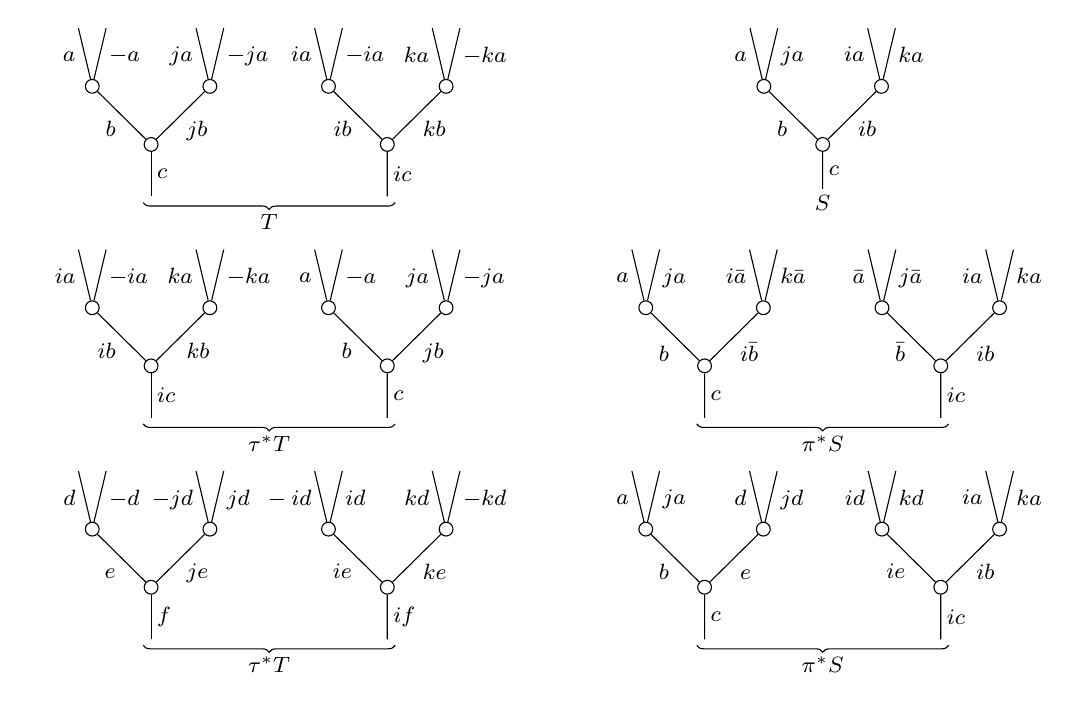
\begin{tikzpicture}[grow=up,auto,level distance=2.1em,
	every node/.style = {font=\footnotesize,inner sep =2pt},
	dummy/.style={circle,draw,inner sep=0pt,minimum size=1.75mm}]
	\begin{scope}[yshift=12em]
		\node at  (0,0) {}
			child{node [dummy] {}
				child[sibling distance = 4.25em]{node [dummy] {}
					child[sibling distance = 1em]{
					edge from parent node [swap,near end] {$-j a$}}
					child[sibling distance = 1em]{
					edge from parent node [near end] {$j a$}}
				edge from parent node [swap] {$j b$}}
				child[sibling distance = 4.25em]{node [dummy] {}
					child[sibling distance = 1em]{
					edge from parent node [swap,near end] {$-a\phantom{j}$}}
					child[sibling distance = 1em]{
					edge from parent node [near end] {$\phantom{j}a$}}
				edge from parent node {$b$}}
			edge from parent node [swap] {$c$}};
		\node at  (3,0) {}
			child{node [dummy] {}
				child[sibling distance = 4.25em]{node [dummy] {}
					child[sibling distance = 1em]{
					edge from parent node [swap,near end] {$- k a$}}
					child[sibling distance = 1em]{
					edge from parent node [near end] {$k a$}}
				edge from parent node [swap] {$k b$}}
				child[sibling distance = 4.25em]{node [dummy] {}
					child[sibling distance = 1em]{
					edge from parent node [swap,near end] {$- i a$}}
					child[sibling distance = 1em]{
					edge from parent node [near end] {$i a$}}
				edge from parent node {$i b$}}
			edge from parent node [swap] {$i c$}};
		\draw[decorate,decoration={brace,amplitude=2.5pt}] (3.1,0) -- (-0.1,0) node[midway,inner sep=4pt]{$T$};
	\end{scope}
	\begin{scope}[yshift=4em]
		\node at  (3,0) {}
			child{node [dummy] {}
				child[sibling distance = 4.25em]{node [dummy] {}
					child[sibling distance = 1em]{
					edge from parent node [swap,near end] {$-j a$}}
					child[sibling distance = 1em]{
					edge from parent node [near end] {$j a$}}
				edge from parent node [swap] {$j b$}}
				child[sibling distance = 4.25em]{node [dummy] {}
					child[sibling distance = 1em]{
					edge from parent node [swap,near end] {$-a\phantom{j}$}}
					child[sibling distance = 1em]{
					edge from parent node [near end] {$\phantom{+1}a$}}
				edge from parent node {$b$}}
			edge from parent node [swap] {$c$}};
		\node at  (0,0) {}
			child{node [dummy] {}
				child[sibling distance = 4.25em]{node [dummy] {}
					child[sibling distance = 1em]{
					edge from parent node [swap,near end] {$- k a$}}
					child[sibling distance = 1em]{
					edge from parent node [near end] {$k a$}}
				edge from parent node [swap] {$k b$}}
				child[sibling distance = 4.25em]{node [dummy] {}
					child[sibling distance = 1em]{
					edge from parent node [swap,near end] {$- i a$}}
					child[sibling distance = 1em]{
					edge from parent node [near end] {$i a$}}
				edge from parent node {$i b$}}
			edge from parent node [swap] {$i c$}};
		\draw[decorate,decoration={brace,amplitude=2.5pt}] (3.1,0) -- (-0.1,0) node[midway,inner sep=4pt]{$\tau^{\**}T$};
	\end{scope}
	\begin{scope}[yshift=-4em]
		\node at  (0,0) {}
			child{node [dummy] {}
				child[sibling distance = 4.25em]{node [dummy] {}
					child[sibling distance = 1em]{
					edge from parent node [swap,near end] {$j d$}}
					child[sibling distance = 1em]{
					edge from parent node [near end] {$-j d$}}
				edge from parent node [swap] {$j e$}}
				child[sibling distance = 4.25em]{node [dummy] {}
					child[sibling distance = 1em]{
					edge from parent node [swap,near end] {$-d\phantom{j}$}}
					child[sibling distance = 1em]{
					edge from parent node [near end] {$\phantom{+1}d$}}
				edge from parent node {$\phantom{j}e$}}
			edge from parent node [swap] {$f$}};
		\node at  (3,0) {}
			child{node [dummy] {}
				child[sibling distance = 4.25em]{node [dummy] {}
					child[sibling distance = 1em]{
					edge from parent node [swap,near end] {$-k d$}}
					child[sibling distance = 1em]{
					edge from parent node [near end] {$k d$}}
				edge from parent node [swap] {$k e$}}
				child[sibling distance = 4.25em]{node [dummy] {}
					child[sibling distance = 1em]{
					edge from parent node [swap,near end] {$i d\phantom{j}$}}
					child[sibling distance = 1em]{
					edge from parent node [near end] {$\phantom{+1}-i d$}}
				edge from parent node {$i e$}}
			edge from parent node [swap] {$i f$}};
		\draw[decorate,decoration={brace,amplitude=2.5pt}] (3.1,0) -- (-0.1,0) node[midway,inner sep=4pt]{$\tau^{\**}T$};
	\end{scope}
	\begin{scope}[yshift=12em,xshift=20em]
		\node at  (1.5,0) {$S$}
			child{node [dummy] {}
				child[sibling distance = 4.25em]{node [dummy] {}
					child[sibling distance = 1em]{
					edge from parent node [swap,near end] {$k a$}}
					child[sibling distance = 1em]{
					edge from parent node [near end] {$i a$}}
				edge from parent node [swap] {$i b$}}
				child[sibling distance = 4.25em]{node [dummy] {}
					child[sibling distance = 1em]{
					edge from parent node [swap,near end] {$j a\phantom{j}$}}
					child[sibling distance = 1em]{
					edge from parent node [near end] {$\phantom{j}a$}}
				edge from parent node {$b$}}
			edge from parent node [swap] {$c$}};
	\end{scope}
	\begin{scope}[yshift=4em,xshift=20em]
		\node at  (0,0) {}
			child{node [dummy] {}
				child[sibling distance = 4.25em]{node [dummy] {}
					child[sibling distance = 1em]{
					edge from parent node [swap,near end] {$k \bar{a}$}}
					child[sibling distance = 1em]{
					edge from parent node [near end] {$i \bar{a}$}}
				edge from parent node [swap] {$i \bar{b}$}}
				child[sibling distance = 4.25em]{node [dummy] {}
					child[sibling distance = 1em]{
					edge from parent node [swap,near end] {$j a\phantom{j}$}}
					child[sibling distance = 1em]{
					edge from parent node [near end] {$\phantom{+1}a$}}
				edge from parent node {$\phantom{\bar{b}j}b$}}
			edge from parent node [swap] {$c$}};
		\node at  (3,0) {}
			child{node [dummy] {}
				child[sibling distance = 4.25em]{node [dummy] {}
					child[sibling distance = 1em]{
					edge from parent node [swap,near end] {$k a$}}
					child[sibling distance = 1em]{
					edge from parent node [near end] {$i a$}}
				edge from parent node [swap] {$i b\phantom{\bar{b}}$}}
				child[sibling distance = 4.25em]{node [dummy] {}
					child[sibling distance = 1em]{
					edge from parent node [swap,near end] {$j \bar{a}\phantom{j}$}}
					child[sibling distance = 1em]{
					edge from parent node [near end] {$\phantom{j}\bar{a}$}}
				edge from parent node {$\bar{b}$}}
			edge from parent node [swap] {$i c$}};
		\draw[decorate,decoration={brace,amplitude=2.5pt}] (3.1,0) -- (-0.1,0) node[midway,inner sep=4pt]{$\pi^{\**}S$};
	\end{scope}
	\begin{scope}[yshift=-4em,xshift=20em]
		\node at  (0,0) {}
			child{node [dummy] {}
				child[sibling distance = 4.25em]{node [dummy] {}
					child[sibling distance = 1em]{
					edge from parent node [swap,near end] {$j d$}}
					child[sibling distance = 1em]{
					edge from parent node [near end] {$\phantom{j}d$}}
				edge from parent node [swap] {$e{\phantom{b}}$}}
				child[sibling distance = 4.25em]{node [dummy] {}
					child[sibling distance = 1em]{
					edge from parent node [swap,near end] {$j a\phantom{j}$}}
					child[sibling distance = 1em]{
					edge from parent node [near end] {$\phantom{j}a$}}
				edge from parent node {$\phantom{j}b$}}
			edge from parent node [swap] {$c$}};
		\node at  (3,0) {}
			child{node [dummy] {}
				child[sibling distance = 4.25em]{node [dummy] {}
					child[sibling distance = 1em]{
					edge from parent node [swap,near end] {$k a$}}
					child[sibling distance = 1em]{
					edge from parent node [near end] {$i a$}}
				edge from parent node [swap] {$i b$}}
				child[sibling distance = 4.25em]{node [dummy] {}
					child[sibling distance = 1em]{
					edge from parent node [swap,near end] {$k d\phantom{j}$}}
					child[sibling distance = 1em]{
					edge from parent node [near end] {$\phantom{+1}i d$}}
				edge from parent node {$i e$}}
			edge from parent node [swap] {$i c$}};
		\draw[decorate,decoration={brace,amplitude=2.5pt}] (3.1,0) -- (-0.1,0) node[midway,inner sep=4pt]{$\pi^{\**}S$};
	\end{scope}
	\end{tikzpicture}
\]
\caption{Root pullbacks}
\label{FIGURE}
\end{figure}
\end{example}


\subsection{Outer faces, tall maps, and substitution}\label{OUTTALL SEC}
\label{SUBS SEC}

One of the key ideas needed 
to describe the free operad monad is
%for our description of operads is 
the notion of \textit{substitution} of tree nodes,
a process that we will prefer to repackage in terms of maps of trees.

In preparation for that discussion,
we first recall some basic definitions and results concerning outer subtrees and tree grafting, as in \cite[\S 5]{Pe17}.


\begin{definition}\label{OUTFACE DEF}
	Let $T \in \Omega$ be a tree and 
	$e_1 \cdots e_n =\underline{e} \leq e$ a broad relation in $T$.
	
	We define the \textit{planar outer face $T_{\underline{e} \leq e}$}
	to be the subtree with underlying set those edges $f \in T$ such that
\begin{equation}\label{OUTERFACE EQ}
	f \leq_d e,\quad \forall_i f \nless_d e_i,
\end{equation}
with generating broad relations the relations $f^{\uparrow} \leq f$ for those $f \in T$ satisfying
$\forall_i f\neq e_i$
in addition to (\ref{OUTERFACE EQ}),
and planar structure pulled back from $T$ (in the sense of Remark \ref{PULLPLANAR REM}).

Moreover, inclusions of the form 
$T_{\underline{e} \leq e}
\hookrightarrow T$
are called \emph{planar outer face maps}.
\end{definition}


\begin{remark}
If one forgoes the requirement that $T_{\underline{e} \leq e}$ be equipped with the pulled back planar structure, the inclusion $T_{\underline{e} \leq e} \hookrightarrow T$ is usually called simply an \textit{outer face map}.
\end{remark}


{\color{red} HERE}



\begin{example}
	\[
	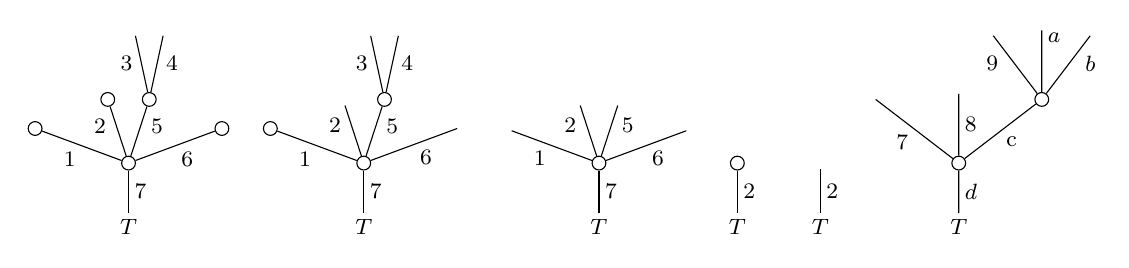
\begin{tikzpicture}[grow=up,auto,level distance=2.3em,
	every node/.style = {font=\footnotesize,inner sep=2pt},
	dummy/.style={circle,draw,inner sep=0pt,minimum size=1.75mm}]
	\node at (0,0) {$T$}
		child[sibling distance = 8em]{node [dummy] {}
			child[sibling distance =2.25em, level distance = 1.25 em]{node [dummy] {}
			edge from parent node [swap] {$6$}}
			child[sibling distance = 1.5em]{node [dummy] {}
				child[sibling distance =1em]{
				edge from parent node [swap,near end] {$4$}}
				child[sibling distance =1em]{
				edge from parent node [near end] {$3$}}
			edge from parent node [very near end,swap] {$5$}}
			child[sibling distance =1.5em]{node [dummy] {}
			edge from parent node [very near end] {$2$}}
			child[sibling distance =2.25em,level distance =1.25em]{node [dummy] {}
			edge from parent node {$1$}}
		edge from parent node [swap] {$7$}};
\begin{scope}[xshift=8.5em]
\node at (0,0) {$T$}
child[sibling distance = 8em]{node [dummy] {}
	child[sibling distance =2.25em, level distance = 1.25 em]{
	edge from parent node [swap] {$6$}}
	child[sibling distance = 1.5em]{node [dummy] {}
		child[sibling distance =1em]{
		edge from parent node [swap,near end] {$4$}}
		child[sibling distance =1em]{
		edge from parent node [near end] {$3$}}
	edge from parent node [very near end,swap] {$5$}}
	child[sibling distance =1.5em]{node {}
	edge from parent node [very near end] {$2$}}
	child[sibling distance =2.25em,level distance =1.25em]{node [dummy] {}
	edge from parent node {$1$}}
edge from parent node [swap] {$7$}};
\end{scope}
\begin{scope}[xshift=17em]
\node at (0,0) {$T$}
child[sibling distance = 8em]{node [dummy] {}
	child[sibling distance =2.25em, level distance = 1.25 em]{node {}
	edge from parent node [swap] {$6$}}
	child[sibling distance = 1.5em]{node {}
	edge from parent node [very near end,swap] {$5$}}
	child[sibling distance =1.5em]{node {}
	edge from parent node [very near end] {$2$}}
	child[sibling distance =2.25em,level distance =1.25em]{node {}
	edge from parent node {$1$}}
edge from parent node [swap] {$7$}};
\end{scope}
\begin{scope}[xshift=22em]
\node at (0,0) {$T$}
child[sibling distance = 8em]{node [dummy] {}
edge from parent node [swap] {$2$}};
\end{scope}
\begin{scope}[xshift=25em]
\node at (0,0) {$T$}
child[sibling distance = 8em]{node {}
	edge from parent node [swap] {$2$}};
\end{scope}
\begin{scope}[xshift=30em]
\node at (0,0) {$T$}
child{node [dummy] {}
	child[sibling distance = 3em]{node [dummy] {}
		child[sibling distance = 1.75em]{
		edge from parent node [near end,swap] {$b$}}
		child[level distance=2.5em]{
		edge from parent node [very near end,swap] {$a$}}				
		child[sibling distance = 1.75em]{
		edge from parent node [near end] {$9$}}
	edge from parent node [swap] {c}}
	child[level distance =2.5em]{
	edge from parent node [swap] {$8$}}
	child[sibling distance = 3em]{
	edge from parent node {$7$}}
edge from parent node [swap] {$d$}};
\end{scope}
	\end{tikzpicture}
	\]
\end{example}


{\color{red} HERE}


We now recap some basic results.


\begin{notation}\label{STICKTRE NOT}
	We write $\eta \in \Omega$
	for the \emph{stick tree} 
	consisting of a single edge and no vertices.
\end{notation}

\begin{proposition}
Let $T \in \Omega$ be a tree.
\begin{itemize}
\item[(a)] $T_{\underline{e} \leq e}$ is a tree with root $e$
and leaf tuple $\underline{e}$;
\item[(b)] there is a bijection
\[
	\{\text{planar outer faces of $T$} \} 
\leftrightarrow 
	\{\text{broad relations of $T$}\};
\]
\item[(c)] if $R \to S$ and $S \to T$ are (planar) outer face maps then so is $R \to T$;
\item[(d)] any pair of broad relations $\underline{g} \leq v$, $\underline{f}v \leq e$ induces a grafting pushout diagram
\begin{equation}\label{GRAPTPUSH EQ}
\begin{tikzcd}
	\eta \ar{r}{v} \ar{d}[swap]{v} & T_{\underline{g} \leq v} \ar{d}
\\
	T_{\underline{f}v \leq e} \ar{r} & T_{\underline{f}\underline{g} \leq e}.
\end{tikzcd}
\end{equation}
Further, $T_{\underline{f} \underline{g} \leq e}$ is the
unique choice of pushout that makes the maps in (\ref{GRAPTPUSH EQ}) planar.
%\item[(e)] a face map $S \to T$ is an outer face map iff whenever the composite relation $\underline{f} \underline{g} \leq e$ is in $S$ then so are the relations $\underline{g} \leq v$ and
%$\underline{f}v \leq e$.
\end{itemize}
\end{proposition}


\begin{proof}
We first show (a). That $T_{\underline{e} \leq e}$ is indeed a tree is the content of \cite[Prop. 5.20]{Pe17}: more precisely, 
$T_{\underline{e} \leq e} = (T^{\leq e})_{\less \underline{e}}$
in the notation therein. That the root of $T_{\underline{e} \leq e}$ is $e$ is clear and that the leaf tuple is $\underline{e}$ follows from \cite[Remark 5.23]{Pe17}.

 (b) follows from (a), which shows that $\underline{e} \leq e$ can be recovered from
$T_{\underline{e} \leq e}$.

 (c) follows from the definition of outer face together with \cite[Lemma 5.33]{Pe17}, which states that the $\leq_d$ relations on $S,T$ coincide.
 
  Since by (b) and (c) both $T_{\underline{g} \leq v}$ and $T_{\underline{f}v \leq e}$ are outer faces of $T_{\underline{f} \underline{g} \leq e}$, 
the first part of (d) is a restatement of \cite[Prop. 5.15]{Pe17}, while the additional planarity claim 
follows by Proposition \ref{PLANARIZATIONCHAR PROP}
together with the vertex identification
$V(T_{\underline{f} \underline{g} \leq e})=
V(T_{\underline{f} v \leq e}) \amalg V(T_{\underline{g} \leq v})$.
%Since $\underline{e} \leq e$ is a broad relation in $T_{\underline{e} \leq e}$ (this follows from (a) together with \cite[Lemma 5.13]{Pe17})
\end{proof}

 
\begin{definition}
	A map $S \xrightarrow{\varphi} T$ in $\Omega$ is called a \textit{tall map} if 
	\[\varphi(\underline{l}_S) = \underline{l}_T, 
		\qquad
	\varphi(r_S)= r_T,\]
where $l_{(\minus)}$ denotes the (unordered) leaf tuple and $r_{(\minus)}$ the root.
\end{definition}


The following is a restatement of \cite[Cor. 5.24]{Pe17}

\begin{proposition}\label{TALLOUTERDEC PROP}
	Any map $S \xrightarrow{\varphi} T$ in $\Omega$ has a factorization, unique up to unique isomorphism,
	\[
		S \xrightarrow{\varphi^t} U \xrightarrow{\varphi^u} T
	\]
	as a tall map followed by an outer face (in fact, 
	$U= T_{\varphi(\underline{l}_S) \leq \varphi(r_S)}$).
\end{proposition}

We recall that a face $F \to T$ is called \textit{inner} if it is obtained by iteratively removing inner edges, i.e. edges other than the root or the leaves. In particular, it follows that a face is inner if and only if it is tall. 
The usual degeneracy-face decomposition
(cf. \cite[Lemma 3.1]{MW07} or \cite[Prop. 5.37]{Pe17})
thus combines with Proposition \ref{TALLOUTERDEC PROP} to give the following.


\begin{corollary}
	Any map $S \xrightarrow{\varphi} T$ in $\Omega$ has a factorization, unique up to unique isomorphisms,
\[
	S \xrightarrow{\varphi^-} U
	\xrightarrow{\varphi^i} V
	\xrightarrow{\varphi^u} T
\]
	as a degeneracy followed by an inner face followed by an outer face.
\end{corollary}
	
% \begin{proof}
% 	The factorization can be built by first performing the degeneracy-\-face decomposition and then performing the tall-outer decomposition on the face map.
% \end{proof}


We will find it convenient  throughout to regard the 
groupoid $\Sigma$ of finite sets 
as the subcategory 
$\Sigma \hookrightarrow \Omega$
consisting of \textit{corollas}
(i.e. trees with a single vertex)
and isomorphisms.


\begin{notation}\label{UNIQCOR NOT}
	Given a tree $T \in \Omega$ there is a unique corolla $\mathsf{lr}(T) \in \Sigma$ and planar tall map 
	$\mathsf{lr}(T) \to T$, which we call the 
	\textit{leaf-root} of $T$ (this name is motivated by the equivariant analogue, discussed in \S \ref{LRVERT SEC}).
	Explicitly, the number of leaves of $\mathsf{lr}(T)$ matches that of $T$, together with the inherited order. 
\end{notation}


We now turn to discussing the substitution operation. We start with an example focused on the closely related notion of 
 iterated graftings of trees (as described in (\ref{GRAPTPUSH EQ})).

\begin{example}\label{GRAFTSUB EX}
The trees $U_1, U_2,\cdots, U_6$ on the left below can be grafted to obtain the tree $U$ in the middle.
More precisely (among other possible grafting orders), one has
\begin{equation}\label{UFORMULA EQ}
U = \left(
		\left(
			\left(
				\left(
					\left(U_6 \amalg_a U_2 \right)
				\right) \amalg_a U_1
			\right) \amalg_b U_3
		\right) \amalg_d U_5
	\right) \amalg_c U_4
\end{equation}
\begin{equation}\label{SUBSDATUMTREES EQ}
	\begin{tikzpicture}[grow=up,auto,level distance=2.1em,
	every node/.style = {font=\footnotesize,inner sep=2pt},
	dummy/.style={circle,draw,inner sep=0pt,minimum size=1.375mm}]
\begin{scope}[xshift=-2em]
	\begin{scope}
	\tikzstyle{level 2}=[sibling distance=2.25em]%
	\tikzstyle{level 3}=[sibling distance=1.25em]%
		\node at (-0.25,3.2) {$U_1$}
			child{node [dummy] {}
				child
				child{node [dummy] {}
					child
					child
				}
			edge from parent node {$a$}};
	\end{scope}
		\node at (-0.25,1.5) {$U_2$}
			child{
		edge from parent node {$a$}};
		\node at (1.15,1.5) {$U_3$}
			child{node [dummy] {}
		edge from parent node {$b$}};
	\begin{scope}
	\tikzstyle{level 2}=[sibling distance=0.875em]%
		\node at (2.2,3.2) {$U_4$}
			child{node [dummy] {}
				child{node [dummy] {}}
				child{node [dummy] {}}
			edge from parent node {$c$}};
	\end{scope}
	\begin{scope}
		\tikzstyle{level 2}=[sibling distance=1.25em]%
		\node at (2.5,1.5) {$U_5$}
			child{node [dummy] {}
				child{node[dummy] {}}
				child{
				edge from parent node {$c$}}
			edge from parent node [swap] {$d$}};
	\end{scope}
	\begin{scope}
	\tikzstyle{level 2}=[sibling distance=3.5em]%
	\tikzstyle{level 3}=[sibling distance=2.25em]%
		\node at (1,-1) {$U_6$}
			child{node [dummy] {}
				child[sibling distance = 5em]{node [dummy] {}
					child[sibling distance = 3.5em]{edge from parent node [swap,near end] {$d$} }
					child[sibling distance = 3.5em]{edge from parent node [near end] {$b$} }
				}
				child[sibling distance = 7em]{ edge from parent node {$a$} }
			edge from parent node [swap] {$e$}};
	\end{scope}
\end{scope}
\begin{scope}[yshift=1em]
	\begin{scope}[level distance=2.3em]
	\tikzstyle{level 2}=[sibling distance=3.5em]%
	\tikzstyle{level 3}=[sibling distance=2.25em]%
	\tikzstyle{level 4}=[sibling distance=1.25em]%
	\tikzstyle{level 5}=[sibling distance=0.875em]%
		\node at (5.5,0) {$U$}
			child{node [dummy] {}
				child[sibling distance =5em]{node [dummy] {}
					child[sibling distance =3.5em]{node [dummy] {}
						child{node [dummy] {}
						}
						child{node [dummy] {}
							child{node [dummy] {}}
							child{node [dummy] {}}
						edge from parent node [near end] {$c$}}
					edge from parent node [swap, near end] {$d$}}
					child[sibling distance =3.5em]{node [dummy] {}
					edge from parent node [near end] {$b$}}
				}
				child[sibling distance =7em]{node [dummy] {}
					child
					child{node [dummy] {}
						child
						child
					}
				edge from parent node {$a$}}
			edge from parent node [swap] {$e$}};
	\end{scope}
	\begin{scope}[level distance=2.3em]
	\tikzstyle{level 2}=[sibling distance=2.3em]%
	\tikzstyle{level 4}=[sibling distance=1em]%
		\node at (10,0.3) {$T$}
			child{node [dummy] {}
				child{node [dummy] {}
					child{node [dummy] {}
					edge from parent node [swap] {$c$}}	
				edge from parent node [swap] {$d$}}
				child{node [dummy] {}
				edge from parent node [near end,swap] {$b$}}
				child{node [dummy] {}
					child{node [dummy] {}
						child
						child
						child
					edge from parent node {$a_1$}}
				edge from parent node {$a_2$}}
			edge from parent node [swap] {$e$}};
	\end{scope}
	\draw [->,dashed] (8.6,1.25) -- node {$\varphi$} (7.1,1.25);
\end{scope}
	\end{tikzpicture}
\end{equation}
We now consider the tree $T$, which is built by converting each $U_i$ into the corolla $\mathsf{lr}(U_i)$, and then performing the same grafting operations as in (\ref{UFORMULA EQ}). $T$ can then be regarded as encoding the combinatorics of the iterated grafting in (\ref{UFORMULA EQ}), with alternative ways to reparenthesize
operations in (\ref{UFORMULA EQ}) in bijection with ways to assemble $T$ out of its nodes.


One can now therefore think of the iterated grafting (\ref{UFORMULA EQ}) as being instead encoded by the tree $T$ together with the (unique) planar tall maps $\varphi_i$ below.
\begin{equation}\label{SUBSDATUMTREES2 EQ}
	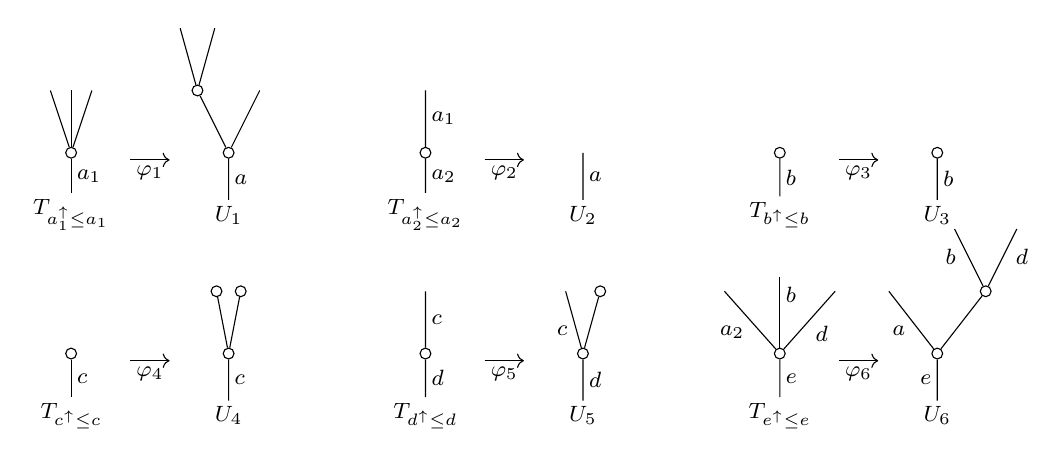
\begin{tikzpicture}[grow=up,auto,level distance=2.25em,
	every node/.style = {font=\footnotesize, inner sep=2pt},
	dummy/.style={circle,draw,inner sep=0pt,minimum size=1.375mm}]
	\begin{scope}
	\tikzstyle{level 2}=[sibling distance=0.75em]%
		\node at (0,0) {$T_{a_1^{\uparrow}\leq a_1}$}
			child{node [dummy] {}
				child
				child
				child
			edge from parent node [swap] {$a_1$}};
	\end{scope}	
	\begin{scope}
	\tikzstyle{level 2}=[sibling distance=2.25em]%
	\tikzstyle{level 3}=[sibling distance=1.25em]%
		\node at (2,0) {$U_1$}
			child{node [dummy] {}
				child
				child{node [dummy] {}
					child
					child
				}
			edge from parent node [swap] {$a$}};
	\end{scope}
		\draw [->] (0.75,0.7) -- node [swap]{$\varphi_1$} (1.25,0.7);
		\node at (4.5,0) {$T_{a_2^{\uparrow}\leq a_2}$}
			child{node [dummy] {}
				child{
				edge from parent node [swap] {$a_1$}}
			edge from parent node [swap] {$a_2$}};
		\node at (6.5,0) {$U_2$}
			child{
			edge from parent node [swap] {$a$}};
		\draw [->] (5.25,0.7) -- node [swap]{$\varphi_2$} (5.75,0.7);
		\node at (9,0) {$T_{b^{\uparrow}\leq b}$}
			child{node [dummy] {}
			edge from parent node [swap] {$b$}};
		\node at (11,0) {$U_3$}
			child{node [dummy] {}
			edge from parent node [swap] {$b$}};
		\draw [->] (9.75,0.7) -- node [swap]{$\varphi_3$} (10.25,0.7);
	\begin{scope}[yshift=-2.55cm]
		\node at (0,0) {$T_{c^{\uparrow}\leq c}$}
			child{node [dummy] {}
			edge from parent node [swap] {$c$}};
	\begin{scope}
	\tikzstyle{level 2}=[sibling distance=0.875em]%
		\node at (2,0) {$U_4$}
			child{node [dummy] {}
				child{node [dummy] {}}
				child{node [dummy] {}}
			edge from parent node  [swap]{$c$}};
	\end{scope}
	\draw [->] (0.75,0.7) -- node [swap]{$\varphi_4$} (1.25,0.7);
		\node at (4.5,0) {$T_{d^{\uparrow}\leq d}$}
			child{node [dummy] {}
				child{
				edge from parent node [swap] {$c$}}
			edge from parent node [swap] {$d$}};
	\begin{scope}
	\tikzstyle{level 2}=[sibling distance=1.25em]%
		\node at (6.5,0) {$U_5$}
			child{node [dummy] {}
				child{node[dummy] {}}
				child{
				edge from parent node {$c$}}
			edge from parent node [swap] {$d$}};
	\end{scope}
	\draw [->] (5.25,0.7) -- node [swap]{$\varphi_5$} (5.75,0.7);
	\begin{scope}
	\tikzstyle{level 2}=[sibling distance=2em]%
		\node at (9,0) {$T_{e^{\uparrow}\leq e}$}
			child{node [dummy] {}
				child{ edge from parent node [swap] {$d$} }
				child[level distance=2.75em]{ edge from parent node [near end,swap] {$b$} }
				child{ edge from parent node {$a_2$} }
			edge from parent node [swap] {$e$}};
	\end{scope}
	\begin{scope}
	\tikzstyle{level 2}=[sibling distance=3.5em]%
	\tikzstyle{level 3}=[sibling distance=2.25em]%
		\node at (11,0) {$U_6$}
			child{node [dummy] {}
				child{node [dummy] {}
					child{ edge from parent node [swap,near end] {$d$} }
					child{ edge from parent node [near end]{$b$} }
				}
				child{ edge from parent node {$a$} }
			edge from parent node {$e$}};
	\end{scope}
	\draw [->] (9.75,0.7) -- node [swap]{$\varphi_6$} (10.25,0.7);
	\end{scope}
	\end{tikzpicture}
\end{equation}
From this perspective, $U$ can now be thought of as obtained from $T$ by \textit{substituting} each of its nodes with the corresponding $U_i$. Moreover, the $\varphi_i$ assemble to a planar tall map 
$\varphi \colon T \to U$ (such that $a_i \mapsto a,b \mapsto b,\cdots,e \mapsto e$), which likewise encodes the same information.

\end{example}

One of the fundamental ideas shaping our perspective on operads
is then that substitution data as in (\ref{SUBSDATUMTREES2 EQ})
can equivalently be repackaged using planar tall maps. 

\begin{definition}\label{SUBSTITUTIONDATUM}
	Let $T \in \Omega$ be a tree.
	
	A \textit{$T$-substitution datum} is a tuple 
	$\left(U_{e^{\uparrow} \leq e}\right)_{(e^{\uparrow} \leq e)\in V(T)}$ together with tall maps
	$T_{e^{\uparrow}\leq e} \to U_{e^{\uparrow}\leq e}$.
	Further, a map of $T$-substitution data 
	$\left(U_{e^{\uparrow} \leq e}\right) \to \left(V_{e^{\uparrow} \leq e}\right)$ is a tuple of tall maps $\left(U_{e^{\uparrow} \leq e}\to V_{e^{\uparrow} \leq e}\right)$ compatible with the substitution maps.
	
	Lastly, a substitution datum is called \textit{planar}
        % a \textit{planar $T$-substitution datum}
        if the chosen maps are planar (so that 
	$\mathsf{lr}(U_{e^{\uparrow} \leq e}) = T_{e^{\uparrow} \leq e}$),
        and a morphism between planar data is called a \textit{planar morphism} if it consists of a tuple of planar maps.
	
	We denote the category of (resp. planar) $T$-substitution data 
	by $\mathsf{Sub}(T)$ (resp. $\mathsf{Sub}_{\mathsf{p}}(T)$).
\end{definition}

\begin{definition}
	Let $T \in \Omega$ be a tree. 
	The \textit{Segal core poset $\mathsf{Sc}(T)$} is the poset with objects the single edge subtrees $\eta_e$ and vertex subtrees $T_{e^{\uparrow} \leq e}$, ordered by inclusion.
\end{definition}


\begin{remark}
Note that the only arrows in $\mathsf{Sc}(T)$ are inclusions of the form $\eta_a \subset T_{e^{\uparrow}\leq e}$.
In particular, there are no pairs of composable non-identity arrows in $\mathsf{Sc}(T)$. 
\end{remark}

Given a $T$-substitution datum $\{U_{\{e^{\uparrow}\leq e\}}\}$ we abuse notation by writing
\[U_{(\minus)} \colon \mathsf{Sc}(T) \to \Omega\]
for the functor $\eta_a \mapsto \eta$, $T_{e^{\uparrow} \leq e} \mapsto U_{e^{\uparrow} \leq e}$  
and sending the inclusions $\eta_a \subset T_{e^{\uparrow} \leq e}$
to the composites
\[
\eta \xrightarrow{a} T_{e^{\uparrow} \leq e}  \to 
%\simeq 
%\mathsf{lr}(U_{e^{\uparrow}\leq e}) \to 
U_{e^{\uparrow} \leq e}.\]


\begin{proposition}\label{SUBDATAUNDERPLAN PROP}
Let $T \in \Omega$ be a tree. There is an isomorphism of categories
\[
\begin{tikzcd}[row sep =0pt]
	\mathsf{Sub}_{\mathsf{p}}(T) \ar[r,shift left=2pt] &
	T \downarrow \Omega^{\mathsf{pt}} \ar[l,shift left=2pt]
\\
	\left(U_{e^{\uparrow} \leq e}\right) \ar[r,mapsto] & 
	\left(T \to \colim_{\mathsf{Sc}(T)} U_{(\minus)}\right)
\\
	\left(U_{\varphi(e^{\uparrow}) \leq \varphi(e)}\right) &
	(T \xrightarrow{\varphi} U) \ar[l,mapsto]
\end{tikzcd}
\]
where $T \downarrow \Omega^{\mathsf{pt}}$ denotes
the category of planar tall maps under $T$
and $\colim_{\mathsf{Sc}(T)} U_{(\minus)}$ is chosen in the unique way that makes the inclusions of the $U_{e^{\uparrow} \leq e}$ planar. 
\end{proposition}


\begin{proof}
We first show in parallel that:
\begin{inparaenum}
\item[(i)] $\colim_{\mathsf{Sc}(T)} U_{(\minus)}$, which we denote $U_T$, exists;
\item[(ii)] for the datum $\left(T_{e^{\uparrow}\leq e}\right)$, it is $T = \colim_{\mathsf{Sc}(T)} T_{(\minus)}$;
\item[(iii)] $V(U_T) = \coprod_{V(T)} V(U_{e^{\uparrow} \leq e})$;
\item[(iv)] the induced map
$T \to U_T$ is planar tall.
\end{inparaenum}
 
The argument is by induction on the number of vertices of $T$, with the base cases of $T$ with $0$ or $1$ vertices being immediate, since then $T$ is the terminal object of $\mathsf{Sc}(T)$.
Otherwise, one can choose a non trivial grafting decomposition so as to write $T = R \amalg_e S$, resulting 
in identifications 
$\mathsf{Sc}(R) \subset \mathsf{Sc}(T)$, 
$\mathsf{Sc}(S) \subset \mathsf{Sc}(T)$
with  % so that 
$\mathsf{Sc}(R) \cup \mathsf{Sc}(S) = \mathsf{Sc}(T)$
and 
$\mathsf{Sc}(R) \cap \mathsf{Sc}(S) = \{\eta_e \}$.
The existence of $U_T = \colim_{\mathsf{Sc}(T)}U_{(\minus)}$
is thus equivalent to the existence of the pushout below
(where the rightmost diagram merely simplifies notation).
\begin{equation}\label{ASSEMBLYGRAFT EQ}
\begin{tikzcd}
	\eta \ar{r}{e} \ar{d}[swap]{e} & \colim_{\mathsf{Sc}(R)}U_{(\minus)} \ar[dashed,d] &
	\eta \ar{r}{e} \ar{d}[swap]{e} & U_R \ar[dashed,d]	
\\
	\colim_{\mathsf{Sc}(S)}U_{(\minus)} \ar[dashed,r] &
	\colim_{\mathsf{Sc}(T)}U_{(\minus)} &
	U_S \ar[dashed,r] &
	U_T
\end{tikzcd}
\end{equation}
By induction, $U_R$ and $U_S$ exist for any $U_{(\minus)}$, 
equal $R$ and $S$ in the case $U_{(\minus)} = T_{(\minus)}$,
$V(U_R) = \coprod_{V(R)} V(U_{e^{\uparrow} \leq e})$
and likewise for $S$ (so that there are unique choices of $U_R$, $U_S$ making the inclusions of $U_{e^{\uparrow} \leq e}$ planar),
and the maps 
$R \to \colim_{\mathsf{Sc}(R)}U_{(\minus)}$,
$S \to \colim_{\mathsf{Sc}(S)}U_{(\minus)}$
are planar tall.
But it now follows that (\ref{ASSEMBLYGRAFT EQ}) is a grafting pushout diagram (cf. (\ref{GRAPTPUSH EQ})), so that the pushout indeed exists. The conditions
$T = \colim_{\mathsf{Sc}(T)}T_{(\minus)}$,
$V(U_T) = \coprod_{V(T)} V(U_{e^{\uparrow} \leq e})$, 
and that
$T \to \colim_{\mathsf{Sc}(T)}U_{(\minus)}$
is planar tall follow.

The fact that the two functors in the statement
are inverse to each other is clear from the same inductive argument.
\end{proof}


\begin{corollary}\label{SUBDATAUNDERPLAN COR}
Let $T \in \Omega$ be a tree. The formulas in
Proposition \ref{SUBDATAUNDERPLAN PROP}
give an isomorphism of categories
\[
\begin{tikzcd}[row sep =0pt]
	\mathsf{Sub}(T) \ar[r,shift left=2pt] &
	T \downarrow \Omega^{\mathsf{t}} \ar[l,shift left=2pt]
\end{tikzcd}
\]
where $T \downarrow \Omega^{\mathsf{t}}$ denotes
the category of tall maps under $T$.
\end{corollary}


\begin{proof}
	This is a consequence of Proposition \ref{PLANARPULL PROP} together with the previous result.
	Indeed, Proposition \ref{PLANARIZATIONCHAR PROP} can be restated as saying that isomorphisms $T \to T'$ are in bijection with substitution data consisting of isomorphisms, and thus  bijectiveness of $\mathsf{Sub}(T) \to T \downarrow \Omega^{\mathsf{t}}$ reduces to that in the previous result.
\end{proof}

\begin{remark}\label{VERTEXDECOMP REM}
As noted in the proof of Proposition \ref{SUBDATAUNDERPLAN PROP}, writing $U = \colim_{\mathsf{Sc}(T)}U_{(\minus)}$,
	one has 
\begin{equation}\label{VERTEXDECOMP EQ}
	V(U) = \coprod_{(e^{\uparrow} \leq e) \in V(T)}
	V(U_{e^{\uparrow} \leq e}).
  \end{equation}
    Alternatively, (\ref{VERTEXDECOMP EQ}) can be regarded as a map 
    $\varphi^{\**} \colon V(U) \to V(T)$ induced by the planar tall map 
    $\varphi \colon T \to U$.
    Explicitly, $\varphi^{\**}(U_{u^{\uparrow} \leq u})$ 
    is the unique $T_{t^{\uparrow}\leq t}$ such that
    there is an inclusion of outer faces $U_{u^{\uparrow} \leq u} \hookrightarrow U_{t^{\uparrow} \leq t}$,
    so that $\varphi^{\**}$ indeed depends contravariantly on the tall map $\varphi$.
\end{remark}

\begin{remark}\label{INPPATH REM}
Suppose that $e \in T$ has input path
$I_T(e) = (e=e_n < e_{n-1} < \cdots < e_0)$.
It is intuitively clear that for a tall map 
$\varphi \colon T \to U$ the input path of $\varphi(e)$ is built by gluing input paths in the $U_{t^{\uparrow} \leq t}$. More precisely (and omitting $\varphi$ for readability), one has
\[
	I_U\left(e_n \right) \simeq 
	I_{n-1}(e_n) \amalg_{e_{n-1}} I_{n-2}(e_{n-1})
	\amalg_{e_{n-2}} \cdots
	\amalg_{e_1} I_1(e_0).
\]
where $I_k(\minus)$ denotes the input path in $U_{e_k^{\uparrow} \leq e_k}$.
More formally, this follows from the characterization of 
predecessors in Proposition \ref{INPUTPREDECESSORPROP PROP}(b).
\end{remark}


We end this section with a couple of lemmas that will allow us to reverse the substitution procedure of 
Proposition \ref{SUBDATAUNDERPLAN PROP}
and will be needed in \S \ref{EXTTREE SEC}.
Recall that the single edge tree $\eta \in \Omega$ is called the stick tree,
cf. Notation \ref{STICKTRE NOT}.

\begin{proposition}\label{BUILDABLE PROP}
	Let $U \in \Omega$ be a tree. Then:
\begin{itemize}
	\item[(i)] given non-stick outer subtrees $U_i$ such that 
	$V(U) = \coprod_i V(U_i)$ there is a unique tree $T$ and planar tall map $T \to U$ such that the sets $\{U_i\}$, $\{U_{e^{\uparrow}\leq e}\}$ coincide;
	\item[(ii)] given multiplicities $m_e \geq 1$ for each edge $e \in U$, there is a unique planar degeneracy $\rho \colon T \to U$ such that $\rho^{-1}(e)$ has $m_e$ elements;
	\item[(iii)] planar tall maps $T \to U$ are in bijection with collections $\{U_i\}$ of outer subtrees such that $V(U) = \coprod_i V(U_i)$ and $U_j$ is not an inner edge of any $U_i$ whenever $U_j \simeq \eta$ is a stick.
\end{itemize}
\end{proposition}


\begin{proof}
	We first show (i) by induction on the number of subtrees $U_i$. The base case $\{U_i\}=\{U\}$ is immediate, setting 
	$T= \mathsf{lr}(U)$. Otherwise, $U$ must not be a corolla and letting $e$ be an edge that is both an inner edge of $U$ and a root of some $U_i$, and one can form a grafting pushout diagram
\begin{equation} \label{DECOMPPROOF EQ}
\begin{tikzcd}
	\eta \ar{r}{e} \ar{d}[swap]{e} & U^{\leq e} \ar{d}
\\
	U_{\nless e} \ar{r} & U
\end{tikzcd}
\end{equation}
where $U^{\leq e}$ (resp. $U_{\nless e}$) are the outer faces consisting of the edges $u \leq_d e$ (resp. $u \nless_d e$).
Since there is a unique $U_i$ containing the vertex $e^{\uparrow} \leq e$, 
it follows from the definition of outer face that there is a
non trivial partition 
$\{U_i\} = \{U_i|U_i \hookrightarrow U^{\leq e}\} 
\amalg \{U_i|U_i \hookrightarrow U_{\nless e}\}$. Existence of $T \to U$ now follows from the induction hypothesis. For uniqueness, the condition that no $U_i$ is a stick guarantees that $T$ possesses a single inner edge mapping to $e$, and thus admits a compatible decomposition as in (\ref{DECOMPPROOF EQ}), so that uniqueness too follows from the induction hypothesis.

For (ii), we argue existence by nested induction on the number of vertices $|V(U)|$ and the sum of the multiplicities $m_e$. The base case $|V(U)|=0$, i.e., $U = \eta$ is immediate. Otherwise, writing $m_e = m'_e +1$, one can form a decomposition (\ref{DECOMPPROOF EQ}) where either $|V(U^{\leq e})|,|V(U_{\nless e})|<|V(U)|$ or one of $U^{\leq e},U_{\nless e}$ is $\eta$, so that $T \to U$ can be built via the induction hypothesis. For uniqueness, note first that 
by \cite[Lemma 5.33]{Pe17} each pre-image $\rho^{-1}(e)$ is linearly ordered and by the ``further'' claim in 
\cite[Cor. 5.39]{Pe17} the remaining broad relations are precisely the pre-image of the non-identity relations in $U$, showing that the underlying broad poset of the tree $T$ is unique  up to isomorphism. Strict uniqueness is then 
Proposition \ref{PLANARPULL PROP}.

(iii) follows by combining (i) and (ii). Indeed, any planar tall map $T \to U$ has a unique factorization 
$T \twoheadrightarrow \bar{T} \hookrightarrow U$
as a planar degeneracy followed by a planar inner face, and each  of these maps is classified by the data in (b) and (a).
\end{proof}


\begin{lemma}\label{OUTERFACEUNION LEM}
	Suppose $T_1,T_2 \hookrightarrow T$ are two outer faces with at least one common edge $e$. Then there exists an unique outer face $T_1 \cup T_2$ such that 
	$V(T_1 \cup T_2) = V(T_1) \cup V(T_2)$.
\end{lemma}

\begin{proof}
	The result is obvious if either
	$T$ is a corolla or if one of $T_1,T_2$
	is one of the root or leaf stick subtrees.

	Otherwise, one can necessarily choose $e$ to be an inner edge of $T$, in which case all three of $T_1,T_2,T$ admit compatible decompositions as in (\ref{DECOMPPROOF EQ}) and the result follows by induction on $|V(T)|$.
\end{proof}



\subsection{Equivariant leaf-root and vertex functors}\label{LRVERT SEC}


This section introduces two functors that are central to our definition of the category $\mathsf{Op}_G$ of
genuine equivariant operads: the leaf-root and vertex functors.

We start by recalling a key class of maps of $G$-trees.


\begin{definition}\label{QUOT DEF}
	Let $S = (S_y)_{y \in Y}$ and $T = (T_x)_{x \in X}$
	be $G$-trees.
	A map of $G$-trees 
	\[
	\varphi = (\phi, (\varphi_y))\colon S \to T
	\]
	is called a \textit{quotient} if each of the constituent tree maps
	\[
	\varphi_y \colon S_y \to T_{\phi(y)}
	\]
is an isomorphism of trees.	

The category of $G$-trees and quotients is denoted $\Omega_{G}^0$ (this notation is justified in \S \ref{PLANARSTRING SEC}).
\end{definition}


\begin{remark}
	Quotients can alternatively be described as the cartesian arrows for the Grothendieck fibration
	$\Omega_G \xrightarrow{\mathsf{r}} \mathsf{O}_G$.
	We note that this is strictly more general than the notion of root pullbacks (Figure \ref{FIGURE}), which are the \textit{chosen} cartesian arrows: those quotients such that each
	$\varphi_y \colon S_y \to T_{\phi(y)}$
	is a planar isomorphism, i.e., an identity.
\end{remark}


\begin{definition}
	The \textit{$G$-symmetric category},
	whose objects we call \textit{$G$-corollas}, is the full subcategory 
	$\Sigma_G \hookrightarrow \Omega_{G}^0$ of those $G$-trees
	$C = (C_x)_{x \in X}$ such that some (and thus all) $C_x$ is a corolla $C_x \in \Sigma \hookrightarrow \Omega$
	(cf. Notation \ref{UNIQCOR NOT}).
\end{definition}


\begin{definition}
	The \textit{leaf-root functor} is the functor $\Omega_{G}^0 \xrightarrow{\mathsf{lr}} \Sigma_G$ defined by 
\[
	\mathsf{lr}\left((T_x)_{x \in X}\right)=
	\left(\mathsf{lr}(T_x)\right)_{x \in X}.
\]
\end{definition}


\begin{remark}
	The leaf-root functor extends 
	to a functor $\mathsf{lr} \colon \Omega^{\mathsf{t}}_G \to \Sigma_G$, 
	where $\Omega^{\mathsf{t}}_G$ is the category of tall maps, defined exactly as in Definition \ref{QUOT DEF}, but not to a functor defined on all arrows in $\Omega_G$.
	Nonetheless, we will be primarily interested in the 
 restriction  
	$\Omega_{G}^0 \xrightarrow{\mathsf{lr}} \Sigma_G$.
\end{remark}

\begin{remark}\label{LEAFROOTEXAMP REM}
	Generalizing the remark in Notation \ref{UNIQCOR NOT},
	$\mathsf{lr}(T)$ can alternatively be characterized as being the \textit{unique} $G$-corolla which admits an also unique planar tall map $\mathsf{lr}(T) \to T$. Moreover, $\mathsf{lr}(T)$ can usually be regarded as the ``smallest inner face'' of $T$, obtained by removing all the inner edges, although this characterization fails when 
	$T=(\eta_x)_{x \in X}$ is a stick $G$-tree. Some examples with $G=\mathbb{Z}_{/4}$ follow.
\[
	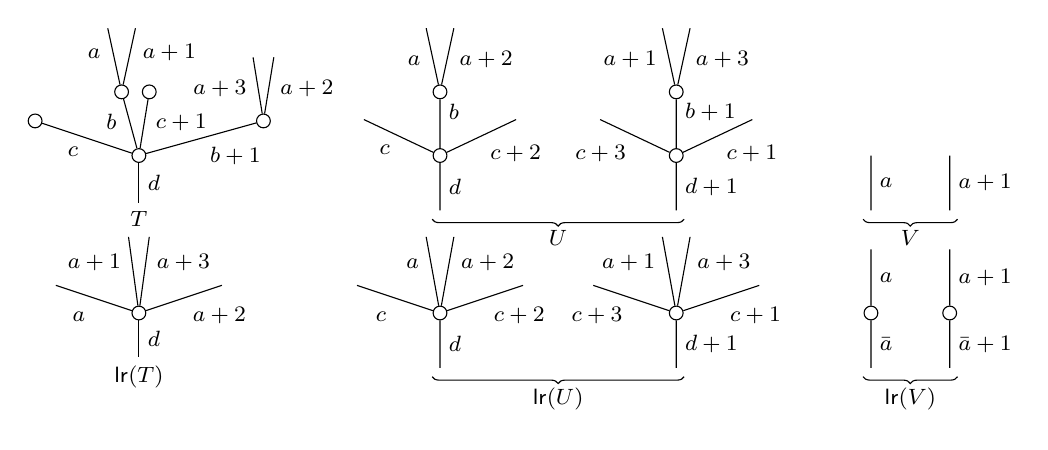
\begin{tikzpicture}[grow=up,auto,level distance=2.3em,
	every node/.style = {font=\footnotesize,inner sep=3pt},
	dummy/.style={circle,draw,inner sep=0pt,minimum size=1.75mm}]
		\node at (0,0) {$T$}
			child{node [dummy] {}
				child[level distance=1.25em,sibling distance = 3em]{node [dummy] {}
					child[level distance=2.3em,sibling distance =0.75em]{
					edge from parent node [swap,near end] {$a+2$}}
					child[level distance=2.3em,sibling distance =0.75em]{
					edge from parent node [near end] {$a+3$}}
				edge from parent node [swap] {$b+1$}}
				child[sibling distance = 0.75em]{node [dummy] {}
				edge from parent node [swap, very near end] {$c+1$}}
				child[sibling distance = 1.25em]{node [dummy] {}
					child[sibling distance = 1em]{
					edge from parent node [swap,very near end] {$a+1$}}
					child[sibling distance = 1em]{
					edge from parent node [very near end] {$\phantom{1+}a$}}
				edge from parent node [very near end] {$b$}}
				child[level distance=1.25em,sibling distance = 2.5em]{node [dummy] {}
				edge from parent node {$c$}}
			edge from parent node [swap] {$d$}};
		\node at (0,-2) {$\mathsf{lr}(T)$}
			child{node [dummy] {}
				child[sibling distance=2em, level distance=1em]{
				edge from parent node [swap] {$a+2$}}
				child[sibling distance=0.75em,level distance=2.75em]{
				edge from parent node [very near end,swap] {$a+3$}}
				child[sibling distance=0.75em,level distance=2.75em]{
				edge from parent node [very near end] {$a+1$}}
				child[sibling distance=2em, level distance=1em]{
				edge from parent node {$\phantom{1+}a$}}
			edge from parent node [swap] {$d$}};
	\begin{scope}[xshift=-0.5em]
		\node at (4,0) {}
			child{node [dummy] {}
				child[level distance=1.3em,sibling distance=2.75em]{
				edge from parent node [swap] {$c+2$}}
				child{node [dummy] {}
					child[sibling distance=1em]{
					edge from parent node [near end,swap] {$a+2$}}
					child[sibling distance=1em]{
					edge from parent node [near end] {$\phantom{1}a$}}
				edge from parent node [swap, near end] {$b$}}
				child[level distance=1.3em,sibling distance=2.75em]{
				edge from parent node {$c$}}
			edge from parent node [swap] {$d$}};
		\node at (7,0) {}
			child{node [dummy] {}
				child[level distance=1.3em,sibling distance=2.75em]{
				edge from parent node [swap] {$c+1$}}
				child{node [dummy] {}
					child[sibling distance=1em]{
					edge from parent node [near end,swap] {$a+3$}}
					child[sibling distance=1em]{
					edge from parent node [near end] {$a+1$}}
				edge from parent node [swap, near end] {$b+1$}}
				child[level distance=1.3em,sibling distance=2.75em]{
				edge from parent node {$c+3$}}
			edge from parent node [swap] {$d+1$}};
			\draw[decorate,decoration={brace,amplitude=2.5pt}] (7.1,0) -- (3.9,0) node[midway,inner sep=4pt]{$U$};
		\node at (4,-2) {}
			child{node [dummy] {}
				child[sibling distance=2em, level distance=1em]{
				edge from parent node [swap] {$c+2$}}
				child[sibling distance=1em,level distance=2.75em]{
				edge from parent node [very near end,swap] {$a+2$}}
				child[sibling distance=1em,level distance=2.75em]{
				edge from parent node [very near end] {$\phantom{1+}a$}}
				child[sibling distance=2em, level distance=1em]{
				edge from parent node {$\phantom{1+}c$}}
			edge from parent node [swap] {$d$}};
		\node at (7,-2) {}
			child{node [dummy] {}
				child[sibling distance=2em, level distance=1em]{
				edge from parent node [swap] {$c+1$}}
				child[sibling distance=1em,level distance=2.75em]{
				edge from parent node [very near end,swap] {$a+3$}}
				child[sibling distance=1em,level distance=2.75em]{
				edge from parent node [very near end] {$a+1$}}
				child[sibling distance=2em, level distance=1em]{
				edge from parent node {$\phantom{1+}c+3$}}
			edge from parent node [swap] {$d+1$}};
\draw[decorate,decoration={brace,amplitude=2.5pt}] (7.1,-2) -- (3.9,-2) node[midway,inner sep=4pt]{$\mathsf{lr}(U)$};
	\end{scope}
	\begin{scope}[xshift=-2em]
			\node at (10,0) {}
				child{
				edge from parent node [swap] {$a$}};
			\node at (11,0) {}
				child{
				edge from parent node [swap] {$a+1$}};
\draw[decorate,decoration={brace,amplitude=2.5pt}] (11.1,0) -- (9.9,0) node[midway,inner sep=4pt]{$V$};
			\node at (10,-2) {}
				child{node[dummy]{}
					child{
					edge from parent node [swap] {$a$}}
				edge from parent node [swap] {$\bar{a}$}};
			\node at (11,-2) {}
				child{node[dummy]{}
					child{
					edge from parent node [swap] {$a+1$}}
				edge from parent node [swap] {$\bar{a}+1$}};
\draw[decorate,decoration={brace,amplitude=2.5pt}] (11.1,-2) -- (9.9,-2) node[midway,inner sep=4pt]{$\mathsf{lr}(V)$};
	\end{scope}
	\end{tikzpicture}
\]	
\end{remark}


\begin{remark}\label{LRROOTMAP REM}
	Since planarizations can not be pushed forward along tree maps (cf. Remark \ref{PULLPLANAR REM})
the leaf-root functor $\mathsf{lr} \colon \Omega_{G}^0 \to \Sigma_G$ is not a Grothendieck fibration,
but instead only a map of Grothendieck fibrations over $\mathsf{O}_G$ 
(for the obvious root functor $\mathsf{r} \colon \Sigma_G \to \mathsf{O}_G$).
\end{remark}


\begin{definition}\label{VG DEF}
Given $T = (T_x)_{x \in X} \in \Omega_G$ we define its set of \textit{vertices} to be $V(T) = \coprod_{x \in X} V(T_x)$
and its set of
	\textit{$G$-vertices} to be the orbit set $V(T)/G$.
	
Furthermore, we will regard 
$V(T)$ as an object of $\Fin$ by using the induced planar order
(with $e^{\uparrow}\leq e$ ordered according to $e$)
and likewise $V_G(T)$ will be regarded as an object of $\Fin$ by using the lexicographic order: i.e. vertex equivalence classes 
$[e^{\uparrow} \leq e]$ are ordered according to the planar order $\leq_p$ of the smallest representative $ge$, $g \in G$.
\end{definition}


\begin{remark}\label{VERTEXDECOMPG REM}
	Following Remark \ref{VERTEXDECOMP REM},
	a tall map $\varphi \colon T \to U$ of $G$-trees
	induces a $G$-equivariant map
	$\varphi^{\**} \colon V(U) \to V(T)$
	and thus also a map of orbits
	$\varphi^{\**} \colon V_G(U) \to V_G(T)$.
	We note, however, that $\varphi^{\**}$ is not in general compatible with the order on $V_G(\minus)$ even if $\varphi$ is planar, as is indeed the case even in the non-equivariant setting.

A minimal example follows.
		\[
		\begin{tikzpicture}[grow=up,auto,level distance=2.2em,
		every node/.style = {font=\footnotesize},
		dummy/.style={circle,draw,inner sep=0pt,minimum size=1.75mm}]
		\node at (0,0) {$T$}
			child{node [dummy] {}
				child[sibling distance = 3.5em]{node [dummy] {}
					child
				edge from parent node[swap] {$c$}}
				child[level distance=2.9em]{
				edge from parent node [swap] {$b$}}
				child[sibling distance = 3.5em]{node [dummy] {}
					child
				edge from parent node {$a$}}		
			edge from parent node [swap] {$d$}};
		\node at (6,0) {$U$}
			child{node [dummy] {}
				child[sibling distance = 5em]{node [dummy] {}
					child
				edge from parent node [swap] {$c$}}
				child[sibling distance = 5em]{node [dummy] {}
					child[sibling distance = 3.5em]{
					edge from parent node [swap,near end] {$b$}}
					child[sibling distance = 3.5em]{node [dummy] {}
						child
					edge from parent node [near end]{$a$}}
				edge from parent node {$e$}}
			edge from parent node [swap] {$d$}};
		\draw[->] (2.1,1) -- node [above] {$\varphi$} (3.8,1) ;
		\end{tikzpicture}
		\]
In $V(T)$ the vertices are ordered as $a<c<d$ while in $V(U)$ they are ordered as $a<e<c<d$ but the map 
$\varphi^{\**} \colon V(U) \to V(T)$ is given by 
$a \mapsto a, c \mapsto c, d \mapsto d, e \mapsto d$.
\end{remark}


\begin{notation}\label{GVERT NOT}
Given $T=(T_x)_{x \in X} \in \Omega_G$
and $(e^{\uparrow} \leq e) \in V(T)$ 
we write $T_{e^{\uparrow}\leq e}$
as a shorthand for $T_{x,e^{\uparrow}\leq e}$, where $e \in T_x$.

Further, each element of $V_G(T)$ corresponds to an unique edge orbit $Ge$ for $e$ not a leaf.
We will prefer to write $G$-vertices as $v_{Ge}$\index{Gvertex@$v_{Ge}$}, 
and write
\begin{equation}\label{TVGE DEF}
	T_{v_{Ge}}\index{Gvertexsubtree@$T_{v_{Ge}}$} = (T_{f^{\uparrow} \leq f})_{f \in Ge}
\end{equation}
where $Ge$ inherits the planar order.
\end{notation}


We note that $T_{v_{Ge}}$ is always a $G$-corolla, leading to the following definition.

\begin{definition}
The \textit{$G$-vertex functor} is the functor
\[
	\begin{tikzcd}[row sep=0]
	\Omega_{G}^0 \ar{r}{V_G} & \Fin_s \wr \Sigma_G \\
	T \ar[mapsto]{r} & (T_{v_{Ge}})_{v_{Ge} \in V_G(T)},
	\end{tikzcd}	
\]
where $\Fin_s$ is the category of finite sets and surjections of
Remark \ref{FINSURJ REM}.
\end{definition}

\begin{remark}
	Note that though the composite
	$\Omega_G^0 \to \Fin_s \wr \Sigma_G \to \Fin_s$
	coincides on objects with the functor described in Remark \ref{VERTEXDECOMPG REM},
	the variance is now reversed. 
\end{remark}

\begin{remark}\label{NEED_WREATH_REMARK}
	In the non-equivariant case the vertex functor can be defined to land instead in $\Sigma \wr \Sigma$.
	The need to introduce the $\Fin_s \wr (\minus)$ construction comes from the fact that
	in general quotient maps do not preserve the number of $G$-vertices.
	As an example,
	let $G=\{\pm 1, \pm i, \pm j, \pm k\}$ and consider the pullback map 
	$\varphi \colon \pi^{\**} S \to S$ of Example \ref{ROOTPULL EX}
	determined by the assignments
	$a \mapsto a$, $b \mapsto b$, $c \mapsto c$, $d \mapsto i a$, $e \mapsto i b$,	
	and presented below in orbital notation. 
		\[
		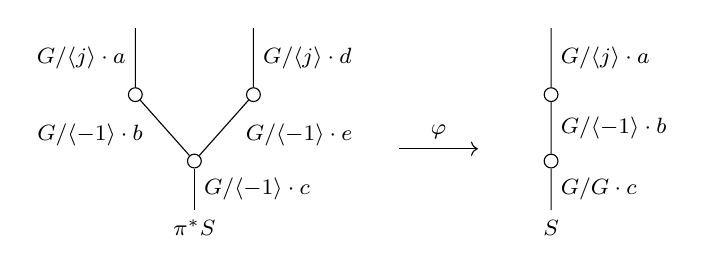
\begin{tikzpicture}[grow=up,auto,level distance=2.4em,every node/.style = {font=\footnotesize},dummy/.style={circle,draw,inner sep=0pt,minimum size=1.75mm}]
		\node at (0,0) {$\pi^{\**}S$}
			child{node [dummy] {}
				child{node [dummy] {}
					child{
					edge from parent node [swap] {$G/\langle j \rangle  \cdot d$}}
				edge from parent node[near end,swap] {$G/\langle -1 \rangle  \cdot e$}}
				child{node [dummy] {}
					child{
					edge from parent node {$G/\langle j \rangle  \cdot a$}}
				edge from parent node [near end] {$G/\langle -1 \rangle  \cdot b$}}		
			edge from parent node[swap] {$G/\langle -1 \rangle  \cdot c$}};
		\node at (4.53,0) {$S$}
			child{node [dummy] {}
				child{node [dummy] {}
					child{
					edge from parent node [swap] {$G/\langle j \rangle \cdot a$}}
				edge from parent node [swap] {$G / \langle -1 \rangle \cdot b$}}
			edge from parent node [swap] {$G/G \cdot c$}};
		\draw[->] (2.6,1) -- node [above] {$\varphi$} (3.6,1) ;
		\end{tikzpicture}
		\]
Note that $T = \pi^{\**} S$ has three $G$-vertices $v_{G c}$, $v_{G b}$, $v_{G e}$ while $S$ has only two $G$-vertices $v_{G c}$ and $v_{G b}$. $V_G(\varphi)$ then maps the two $G$-corollas 
$T_{v_{G b}}$ and $T_{v_{G e}}$
isomorphically onto $S_{v_{G b}}$
and the $G$-corolla $T_{v_{Gc}}$ by a non-isomorphism quotient onto $S_{v_{G c}}$.
\end{remark}


The following elementary statement will play an important auxiliary role.


\begin{lemma}\label{VGPULL LEM}
The $G$-vertex functor
\[
\begin{tikzcd}
	\Omega_{G}^0 \ar{r}{V_G} & \Fin_s \wr \Sigma_G
\end{tikzcd}
\]
sends pullbacks over $\mathsf{O}_G$ (i.e. root pullbacks)
to pullbacks over $\Fin_s \wr \mathsf{O}_G$
(cf. Lemma \ref{FWRGROTH LEM}).
\end{lemma}

\begin{proof}
Note first that an arrow 
$(\phi,(\varphi_i))\colon (C_i)_{i \in I} \to (C'_j)_{j\in J}$
is a pullback for the split fibration 
$\Fin_s \wr \Sigma_G \to \Fin_s \wr \mathsf{O}_G$
iff each of the constituent arrows
$\varphi_i \colon C_i \to C'_{\phi(i)}$
are pullbacks for the split fibration $\Sigma_G \to \mathsf{O}_G$.

The pullback
$\psi^{\**} T \xrightarrow{\bar{\psi}} T$
of $T = (T_x)_{x \in X} \in \Omega_{G}^{0}$
over $\psi \colon Y \to X$
has the form 
$(T_{\psi(y)})_{y \in Y} \to (T_x)_{x \in X}$
and it now suffices to check that each of the vertex maps
$
	(\psi^{\**} T)_{v_{G e}} \to T_{v_{G \bar{\psi}(e)}}
$
is itself a pullback.
By (\ref{TVGE DEF}), this is the statement that for 
$f \in G e$ the induced map
\begin{equation}\label{VGPULL EQ}
	(\psi^{\**}T)_{f^{\uparrow} \leq f} \to 
	T_{\bar{\psi}(f^{\uparrow}) \leq \bar{\psi} (f)}
\end{equation}
is an identity (i.e. planar isomorphism),
and letting $y$ be such that $f \in T_{\psi(y)}$
one sees that (\ref{VGPULL EQ})
is the identity
$T_{\psi(y),f^{\uparrow} \leq f} = 
T_{x,\bar{\psi}(f)^{\uparrow} \leq \bar{\psi}(f)}$, where $x=\psi(y)$, finishing the proof.
\end{proof}


\begin{example}
The following depicts one of the maps 
(\ref{VGPULL EQ})
for the pullback $\tau^{\**} T \to T$
in Example \ref{ROOTPULL EX}.
\[
	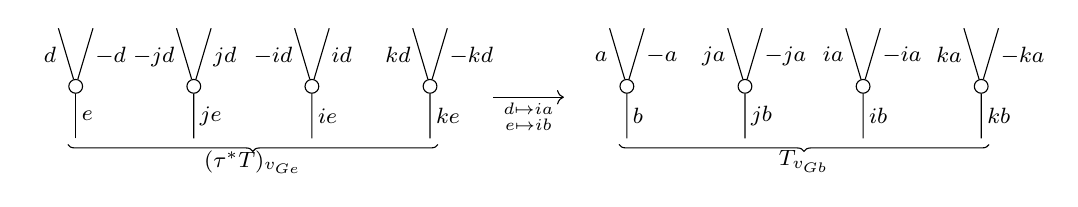
\begin{tikzpicture}[grow=up,auto,level distance=2.1em,
	every node/.style = {font=\footnotesize,inner sep=2pt},
	dummy/.style={circle,draw,inner sep=0pt,minimum size=1.75mm}]
	\begin{scope}[xshift=7cm]
		\node at (0,0) {}
			child{node [dummy] {}
				child[sibling distance=1.25em]{
				edge from parent node [swap,near end] {$-a\phantom{j}$}}
				child[sibling distance=1.25em]{
				edge from parent node [near end]  {$\phantom{j}a$}}
			edge from parent node [swap] {$b$}};
		\node at (1.5,0) {}
			child{node [dummy] {}
				child[sibling distance=1.25em]{
				edge from parent node [swap,near end] {$-j a$}}
				child[sibling distance=1.25em]{
				edge from parent node [near end]  {$j a$}}
			edge from parent node [swap] {$j b$}};
		\node at (3,0) {}
			child{node [dummy] {}
				child[sibling distance=1.25em]{
				edge from parent node [swap,near end] {$-i a$}}
				child[sibling distance=1.25em]{
				edge from parent node [near end]  {$i a$}}
			edge from parent node [swap] {$i b$}};
		\node at (4.5,0) {}
			child{node [dummy] {}
				child[sibling distance=1.25em]{
				edge from parent node [swap,near end] {$-k a$}}
				child[sibling distance=1.25em]{
				edge from parent node [near end]  {$k a$}}
			edge from parent node [swap] {$k b$}};
		\draw[decorate,decoration={brace,amplitude=2.5pt}] (4.6,0) -- (-0.1,0) node[midway]{$T_{v_{G b}}$};
	\end{scope}
		\node at (0,0) {}
			child{node [dummy] {}
				child[sibling distance=1.25em]{
				edge from parent node [swap,near end] {$-d\phantom{j}$}}
				child[sibling distance=1.25em]{
				edge from parent node [near end]  {$\phantom{j}d$}}
			edge from parent node [swap] {$e$}};
		\node at (1.5,0) {}
			child{node [dummy] {}
				child[sibling distance=1.25em]{
				edge from parent node [swap,near end] {$j d$}}
				child[sibling distance=1.25em]{
				edge from parent node [near end]  {$-j d$}}
			edge from parent node [swap] {$j e$}};
		\node at (3,0) {}
			child{node [dummy] {}
				child[sibling distance=1.25em]{
				edge from parent node [swap,near end] {$i d$}}
				child[sibling distance=1.25em]{
				edge from parent node [near end]  {$-i d$}}
			edge from parent node [swap] {$i e$}};
		\node at (4.5,0) {}
			child{node [dummy] {}
				child[sibling distance=1.25em]{
				edge from parent node [swap,near end] {$-k d$}}
				child[sibling distance=1.25em]{
				edge from parent node [near end]  {$k d$}}
			edge from parent node [swap] {$k e$}};
		\draw[decorate,decoration={brace,amplitude=2.5pt}] (4.6,0) -- (-0.1,0) node[midway]{$(\tau^{\**}T)_{v_{G e}}$};
	\draw[->] (5.3,0.6) -- node [below] {$\substack{d \mapsto i a \\ e \mapsto i b}{}$} (6.2,0.6) ;
	\end{tikzpicture}
\]
Note that 
$(\tau^{\**} T)_{v_{G e}} = \rho^{\**} T_{v_{G b}}$
for $\rho$ the map
$\{e,j e, i e, k e\} \to \{b, j b, i b, k b\}$ 
defined by $e \mapsto i b$ so that,
accounting for orders,
$\rho$ is the block permutation $\rho = (13)(24)$.
\end{example}


We are now in a position to generalize 
Definition \ref{SUBSTITUTIONDATUM}.

\begin{definition}\label{SUBSTITUTIONDATUMG DEF}
	Let $T \in \Omega_G$ be a $G$-tree.
	
	A \textit{(resp. planar) $T$-substitution datum} is a tuple 
	$\left(U_{f^{\uparrow} \leq f} \right)_{V(T)}$ of trees together with
\begin{itemize}	
\item[(i)] associative and unital $G$-action maps
$U_{f^{\uparrow} \leq f} \to U_{g f^{\uparrow} \leq g f}$; 
\item[(ii)]	(planar) tall maps 
	$T_{f^{\uparrow} \leq f} \to U_{f^{\uparrow} \leq f}$ compatible with the $G$-action maps.
\end{itemize}	
	Further, a map of (planar) $T$-substitution data 
	$\left(U_{f^{\uparrow} \leq f}\right) \to
	\left(V_{f^{\uparrow} \leq f}\right)$ is a compatible tuple of (planar) tall maps 
	$\left(U_{f^{\uparrow} \leq f} \to V_{f^{\uparrow} \leq f} \right)$.
	
	We denote the category of (planar) $T$-substitution data 
	by $\mathsf{Sub}(T)$
	(resp. $\mathsf{Sub}_{\mathsf{p}}(T)$).
\end{definition}


Recall that a map of $G$-trees is called 
\textit{rooted} if it induces an ordered isomorphism on the root orbit (cf. Definition \ref{ROOTPULL DEF}),
and we note that by Definition \ref{PLANARMAP_DEF} planar tall maps of $G$-trees are always rooted.

\begin{remark}\label{SUBSGREF DEF}
Writing $U^{\mathsf{r}}_{v_{G e}} = (U_{f^{\uparrow} \leq f})_{f \in Ge}$
a $T$-substitution datum can equivalently be encoded by the tuple
$\left(U^{\mathsf{r}}_{v_{G e}}\right)_{V_G(T)}$ together with \textit{rooted} tall maps 
$T_{v_{Ge}} \to U^{\mathsf{r}}_{v_{G e}}$.
The need to include $\mathsf{r}$ (which stands for ``rooted'')
in the notation is explained by Remark \ref{WHYR REM}.

Further, the $T$-substitution datum is planar iff the maps $T_{v_{Ge}} \to U^{\mathsf{r}}_{v_{G e}}$ are as well.
\end{remark}


\begin{remark}\label{SUBSDATUMCONV REM}
%	To establish the equivariant analogue of Proposition \ref{SUBDATAUNDERPLAN PROP} we first repackage equivariant substitution data in terms of non-equivariant ones.
%
%	The rooted condition of $T$-substitution data allows us to write
%	$U_{v_{G e}} = (U_{f^{\uparrow} \leq f})_{f \in v_{Ge}}$
%	for each $v_{G e} \in V_G(T)$, 
	Writing $T = (T_x)_{x \in X}$ as usual
	one obtains (non-equivariant) $T_x$-substitution data 
	$U_{x,(\minus)}$ for each $T_x$.
	We again write
	$U_{x,(\minus)} \colon \mathsf{Sc}(T_x) \to \Omega$
	and note that these are compatible with the $G$-action in the sense that the obvious diagram
\[
\begin{tikzcd}[row sep =3pt]
	\mathsf{Sc}(T_x) \ar{rr}{U_{x,(\minus)}} \ar{rd}[swap]{g} &&
	\Omega
\\
	& \mathsf{Sc}(T_{gx}) \ar{ru}[swap]{U_{gx,(\minus)}}
\end{tikzcd}
\]
commutes.
Writing $\mathsf{Sc}(T) = \coprod_x \mathsf{Sc}(T_x)$,
these diagrams assemble into a functor
$G \ltimes \mathsf{Sc}(T) \to \Omega$,
where $G \ltimes \mathsf{Sc}(T)$ is the Grothendieck construction for the $G$-action
(which, explicitly, adds arrows 
$\eta_a \to \eta_{ga}$, 
$T_{e^{\uparrow} \leq e} \to T_{ge^{\uparrow} \leq ge}$
to $\mathsf{Sc}(T)$ that satisfy obvious compatibilities).
\end{remark}


In the following we write
$\colim_{\mathsf{Sc}(T)}U_{(\minus)}$
to mean
$(\colim_{\mathsf{Sc}(T_x)}U_{x,(\minus)})_{x \in X}$ or, in other words, we take the colimit 
in $\Phi = \Fin \wr \Omega$ rather than in $\Omega$
(as is needed since $\Omega$ lacks coproducts).


\begin{corollary}\label{SUBDATAUNDERPLANG COR}
Let $T \in \Omega_G$ be a $G$-tree. There are isomorphisms of categories
\[
\begin{tikzcd}[row sep =0pt]
	\mathsf{Sub}_{\mathsf{p}}(T) \ar[r,shift left=2pt] &
	T \downarrow \Omega_{G}^{\mathsf{pt}} \ar[l,shift left=2pt] &
	\mathsf{Sub}(T) \ar[r,shift left=2pt] &
	T \downarrow \Omega_{G}^{\mathsf{rt}} \ar[l,shift left=2pt]
\\
	\left(U_{f^{\uparrow} \leq f}\right)_{V(T)} \ar[r,mapsto] & 
	\left(T \to \colim_{\mathsf{Sc}(T)} U_{(\minus)}\right) &
	\left(U_{f^{\uparrow} \leq f}\right)_{V(T)} \ar[r,mapsto] & 
	\left(T \to \colim_{\mathsf{Sc}(T)} U_{(\minus)}\right)
\end{tikzcd}
\]
where $T \downarrow \Omega_G^{\mathsf{pt}}$ 
(resp. $T \downarrow \Omega_G^{\mathsf{rt}}$)
is the category of planar tall (resp. rooted tall) maps under $T$.
\end{corollary}


\begin{proof}
	This is a direct consequence of the 
	non-equivariant analogues Proposition \ref{SUBDATAUNDERPLAN PROP} and Corollary \ref{SUBDATAUNDERPLAN COR}
	applied to each individual $T_x$ together with the equivariance analysis in
	Remark \ref{SUBSDATUMCONV REM}.
\end{proof}


\begin{remark} \label{WHYR REM}
Writing $U = \colim_{\mathsf{Sc}(T)}U_{(\minus)}$, 
it follows from the non-equivariant results
Proposition \ref{SUBDATAUNDERPLAN PROP} and
Corollary \ref{SUBDATAUNDERPLAN COR}
that each inclusion map $U_{f^{\uparrow} \leq f} \to U$
is planar, so that there is no conflict with 
Notation \ref{GVERT NOT}.

However, some care is needed concerning the
$U_{v_{Ge}}^{\mathsf{r}}$ appearing in the reformulation of substitution data given in Remark \ref{SUBSGREF DEF}.
Letting $\varphi \colon T \to U$ be the induced map,
one sees that while $U_{v_{Ge}}^{\mathsf{r}}$ and 
$U_{v_{G\varphi(e)}}$
have the same constituent trees (with the latter defined by Notation \ref{GVERT NOT}),
the roots of $U_{v_{Ge}}^{\mathsf{r}}$ are ordered by $Ge$
while those of $U_{v_{G\varphi(e)}}$ are ordered by $G \varphi(e)$.
More succinctly, it is then 
$U_{v_{Ge}}^{\mathsf{r}} = \varphi_{Ge}^{\**}U_{v_{G\varphi(e)}}$ for $\varphi_{Ge} \colon Ge \to G \varphi(e)$
the induced map.

Lastly, we note that such distinctions are unnecessary for planar data, since then the $\varphi_{G e}$ are ordered isomorphisms (i.e. identities), so that 
$U_{v_{Ge}}^{\mathsf{r}} = U_{v_{G\varphi(e)}}$.
\end{remark}

\begin{remark}\label{PULLCOMP REM}
	The isomorphisms in Corollary \ref{SUBDATAUNDERPLANG COR}
	are compatible with root pullbacks of trees. 
	More concretely, as in the proof of Lemma \ref{VGPULL LEM},
	each pullback 
	$\bar{\psi} \colon \psi^{\**} T \to T$
	determines pullback maps
	$\bar{\psi}_{G e} \colon
	(\psi^{\**} T)_{v_{Ge}} \to T_{v_{G \bar{\psi}(e)}}$,
	which we note are pullbacks over the maps
	$\bar{\psi}_{G e} \colon Ge \to G \bar{\psi}(e)$
	in $\mathsf{O}_G$. The definition of pullback then allows us to uniquely fill any diagram (where we reformulate substitution data as in Remark \ref{SUBSGREF DEF})
\[
\begin{tikzcd}[row sep =10pt]
	(\psi^{\**} T)_{v_{Ge}} \ar{d} \ar[dashed]{r} &
	\bar{\psi}_{G e}^{\**}U_{v_{G \bar{\psi}(e)}}^{\mathsf{r}} \ar{d}
\\
	T_{v_{G \bar{\psi}(e)}} \ar{r} &
	U_{v_{G \bar{\psi}(e)}}^{\mathsf{r}}
\end{tikzcd}	
\]
defining the left vertical functors (with the right functors defined analogously) in each of the commutative diagrams below.
\begin{equation}\label{SUBDATAUNDERPLANG2 EQ}
\begin{tikzcd}[row sep =12pt,column sep= 14pt]
	\mathsf{Sub}_{\mathsf{p}}(\psi^{\**} T) \ar[r,shift left=2pt] &
	\psi^{\**} T \downarrow \Omega_{G}^{\mathsf{pt}} \ar[l,shift left=2pt] & &
	\mathsf{Sub}(\psi^{\**} T) \ar[r,shift left=2pt] &
	\psi^{\**} T \downarrow \Omega_{G}^{\mathsf{rt}} \ar[l,shift left=2pt]
\\
	\mathsf{Sub}_{\mathsf{p}}(T) \ar[r,shift left=2pt] \ar{u}{(\bar{\psi}_{Ge}^{\**})} &
	T \downarrow \Omega_{G}^{\mathsf{pt}} \ar[l,shift left=2pt] \ar{u}[swap]{\psi^{\**}} & &
	\mathsf{Sub}(T) \ar[r,shift left=2pt] \ar{u}{(\bar{\psi}_{Ge}^{\**})} &
	T \downarrow \Omega_{G}^{\mathsf{rt}} \ar[l,shift left=2pt] \ar{u}[swap]{\psi^{\**}}
\end{tikzcd}
\end{equation}
\end{remark}


\subsection{Planar strings}\label{PLANARSTRING SEC}

We now use the leaf-root and vertex functors to repackage 
our substitution results in a format that will be more convenient for our definition of genuine equivariant operads in \S \ref{GENUINE_OP_MONAD_SECTION}.


\begin{definition}\label{PLANSTR DEF}
	The category $\Omega_{G}^n$ of 
	\textit{planar $n$-strings} is the category whose objects are strings
\begin{equation}\label{STRINGOBJ EQ}
	\begin{tikzcd}
	T_0 \ar{r}{\varphi_1} & T_1 \ar{r}{\varphi_2} & \cdots \ar{r}{\varphi_n} & T_n
	\end{tikzcd}	
\end{equation}
	where $T_i \in \Omega_G$ and the $\varphi_i$ are planar \textit{tall} maps, while arrows are commutative diagrams 
	\begin{equation} \label{PTNARROW EQ}
	\begin{tikzcd}
	T_0 \ar{r}{\varphi_1} \ar{d}[swap]{\pi_0} & T_1 \ar{r}{\varphi_2} \ar{d}[swap]{\pi_1} & \cdots \ar{r}{\varphi_n} & T_n \ar{d}[swap]{\pi_n}
\\
	T'_0 \ar{r}[swap]{\varphi'_1} & T'_1 \ar{r}[swap]{\varphi'_2} & \cdots \ar{r}[swap]{\varphi'_n} & T'_n
	\end{tikzcd}	
	\end{equation}
where each $\pi_i$ is a quotient map.
\end{definition}

%\begin{remark}
%	While these could be called ``planar tall $n$-strings'', we will never use strings on non-tall maps,
%	and so there is no ambiguity.
%\end{remark}

\begin{notation}\label{SIMPOPERATORS NOT}
	Since compositions of planar tall arrows are planar tall
	and identity arrows are planar tall	
	it follows that 
	$\Omega_{G}^{\bullet}$
	forms a simplicial object in $\mathsf{Cat}$, 
	with faces given by composition and degeneracies by inserting identities. 

	Further setting 
	$\Omega_{G}^{-1} = \Sigma_G$, the leaf-root functor $\Omega_{G}^{0} \xrightarrow{\mathsf{lr}} \Sigma_G$ makes 
	$\Omega_{G}^{\bullet}$ into an augmented simplicial object and, furthermore, the maps 
	$s_{-1} \colon \Omega_{G}^{n} \to \Omega_{G}^{n+1}$
sending $T_0 \to T_1 \to \cdots \to T_n$ to 
$\mathsf{lr}(T_0) \to T_0 \to T_1 \to \cdots \to T_n$ equip it with extra degeneracies.
\end{notation}


\begin{remark}
The identification $\Omega_{G}^{-1} = \Sigma_G$ can be understood by noting that a string as in (\ref{STRINGOBJ EQ}) is equivalent to a string
\begin{equation}\label{STRINGOBJALT EQ}
	\begin{tikzcd}
	T_{-1} \ar{r}{\varphi_0} & T_0 \ar{r}{\varphi_1} & T_1 \ar{r}{\varphi_2} & \cdots \ar{r}{\varphi_n} & T_n
	\end{tikzcd}	
\end{equation}
where $T_{-1} = \mathsf{lr}(T_0) = \cdots = \mathsf{lr}(T_n)$.
\end{remark}


\begin{remark}\label{ALLSPLITMAPS REM}
Since for any planar $n$-string we have 
$\mathsf{r}(T_i) = \mathsf{r}(T_j)$
for any $1 \leq i,j \leq n$, 
there is a well defined functor
$\mathsf{r} \colon \Omega_{G}^{n} \to \mathsf{O}_G$,
which is readily seen to be a split Grothendieck fibration.
Furthermore, generalizing Remark \ref{LRROOTMAP REM},
all operators $d_i$, $s_j$ 
are maps of split Grothendieck fibrations.
\end{remark}


\begin{notation}\label{VGDEF NOT}
We extend the vertex functor to a functor 
$V_G \colon \Omega_{G}^{n} \to \Fin_s \wr \Omega_{G}^{n-1}$
by
\begin{equation}\label{VGDEF EQ}
	V_G(T_0 \to T_1 \to \cdots \to T_n) = 
	(T_{1,v_{Ge}} \to \cdots \to
	T_{n,v_{Ge}})_{v_{Ge} \in V_G(T_0)}	
\end{equation}
where we abuse notation by writing $T_{i,v_{Ge}}$
for 
$(T_{i,\bar{\varphi}_i(f)^{\uparrow}\leq \bar{\varphi}_i(f)})_{f \in Ge}$, where 
$\bar{\varphi}_i = \varphi_i \circ \cdots \circ \varphi_1$.

Alternatively, regarding $T_0 \to \cdots \to T_n$ as a string of $n$ arrows in $T_0 \downarrow \Omega_G^{\mathsf{pt}}$, 
the object $V_G(T_0 \to \cdots \to T_n)$
can be thought of as the image of the inverse functor in
Corollary \ref{SUBDATAUNDERPLANG COR},
written according to the reformulation in 
Remark \ref{SUBSGREF DEF}
(where since we are in the planar case we need not distinguish between the
$U_{(\minus)}^{\mathsf{r}}$ and $U_{(\minus)}$ notations
(cf. Remark \ref{WHYR REM})).
Note however that from this perspective
functoriality needs to be addressed separately.
\end{notation}


\begin{notation}\label{DDDDD NOT}
	For $X \subseteq \{0,1,\cdots,n\}$
	we write
	$d_X \colon \Omega^n_G \to \Omega^{n-|X|}_G$
	for the functor which sends 
	$T_0 \to T_1 \to \cdots \to T_n$
	to the string with $T_x, x\in X$ omitted.
	
	Note that, in light of \eqref{STRINGOBJALT EQ},
	this makes sense even when
	$X = \{0,1,\cdots,n\}$.
\end{notation}

We now obtain a key reinterpretation (and slight strengthening) of Corollary \ref{SUBDATAUNDERPLANG COR}.


\begin{proposition} \label{SUBSASPULL PROP}
For any $n\geq 0$ the commutative diagram
	\begin{equation}\label{PTPULL EQ}
	\begin{tikzcd}
		\Omega_{G}^{n} \ar{r}{V_G} 
		\ar{d}[swap]{d_{1,\cdots,n}} & \Fin_s \wr \Omega_{G}^{n-1} 
		\ar{d}{\Fin \wr d_{0,\cdots,n-1}}
	\\
		\Omega_{G}^{0} \ar{r}[swap]{V_G} & \Fin_s \wr \Sigma_G
	\end{tikzcd}
	\end{equation}
is a pullback diagram in $\mathsf{Cat}$.
\end{proposition}


\begin{proof}
Let us write 
$P = \Omega_{G}^{0} \times_{\Fin_s \wr \Sigma_G} \Fin_s \wr \Omega_{G}^{n-1}$ for the pullback,
so that our goal is to show that the canonical map
$\Omega_{G}^{n} \to P$ is an isomorphism. 

That $\Omega_{G}^{n} \to P$ is an isomorphism on objects 
follows by combining the alternative description of $V_G$
in Notation \ref{VGDEF NOT} with the planar half of
Corollary \ref{SUBDATAUNDERPLANG COR}
(in fact, this yields isomorphisms of the fibers over 
$\Omega_{G}^{0}$, but we will not directly use this fact).
We will hence write $T_0 \to \cdots \to T_n$
to denote an object of $P$ as well.

An arrow in $P$ from 
$T_0 \to \cdots \to T_n$ to 
$T'_0 \to \cdots \to T'_n$
then consists of a quotient 
$\pi_0 \colon T_0 \to T'_0$
together with a $V_G(T_0)$ indexed tuple of quotients of strings (where we write $e'=\pi_0(e)$)
\begin{equation} \label{PTNARROWLOC EQ}
\begin{tikzcd}[column sep=1.2em]
	T_{0,v_{G e}} \ar{r}{} \ar{d}[swap]{\pi_{0,e}} & 
	T_{1,v_{G e}} \ar{r}{} \ar{d}[swap]{\pi_{1,e}} &
	\cdots \ar{r}{} &
	T_{n,v_{G e}} \ar{d}{\pi_{n,e}}
\\
	T'_{0,v_{G e'}} \ar{r}{} &
	T'_{1,v_{G e'}} \ar{r}{} &
	\cdots \ar{r}{} &
	T'_{n,v_{G e'}}.
\end{tikzcd}	
\end{equation}
%Note that the rooted arrows in (\ref{PTNARROWLOC EQ})
%and we note that the dashed information is superfluous
%since $T_{0,v_{G e}} = \mathsf{lr}(T_{1,v_{G e}})$,
%$T'_{0,v_{G e}} = \mathsf{lr}(T'_{1,v_{G e}})$.
That $\Omega_{G}^{n} \to P$ is injective on arrows is then clear.

For surjectivity, note first that by Lemma \ref{VGPULL LEM} the composite $P \to \Omega_{G}^{0} \to \mathsf{O}_G$
is a split Grothendieck fibration and 
$P \to \Omega_{G}^{0}$ is a map of split Grothendieck fibrations. 
Indeed, pullbacks in $P$ can be built explicitly as those arrows such that $\pi_0$ and all $\pi_{i,e}$ in 
(\ref{PTNARROWLOC EQ})
are pullbacks (alternatively, an abstract argument also works).
The alternative description of $V_G$ in 
Notation \ref{VGDEF NOT} combined with
(\ref{SUBDATAUNDERPLANG2 EQ}) 
then show that 
$\Omega_{G}^{n} \to P$ preserves pullback arrows,
so that surjectivity needs only be checked for maps in the fibers over $\mathsf{O}_G$, i.e. on rooted maps.
Tautologically, a map in $P$ is rooted iff $\pi_0 \colon T_0 \to T'_0$ is.
But since a quotient is an isomorphism iff it is so on roots,
we further have that 
a map in $P$ is rooted iff $\pi_0 \colon T_0 \to T'_0$
is a rooted isomorphism and
each $\pi_{i,e}$ in (\ref{PTNARROWLOC EQ}) is an isomorphism.
But now reinterpreting (\ref{PTNARROWLOC EQ}) as a tuple of diagrams indexed by
$f \in G e$
one obtains a diagram in $\mathsf{Sub}(T_0)$ of the same shape  which, once converted to a diagram in 
$T_0 \downarrow \Omega_G^{\mathsf{rt}}$
using the rooted half of Corollary \ref{SUBDATAUNDERPLANG COR},
yields the desired rooted map (\ref{PTNARROW EQ})
in $\Omega_{G}^{n}$ lifting the rooted map in $P$.
\end{proof}


%\begin{remark}\label{DSCOM REM}
%The diagrams (with back and lower slanted faces instances of (\ref{PTPULL EQ}))
%	\[
%	\begin{tikzcd}[column sep = 0.1em]
%		\Omega_{G,{n+1}} \ar{rr} \ar{rd}{d_{i+1}} \ar{dd}
%		 & & \Fin_s \wr \Omega_{G,{n}} \ar{rd}{\Fin_s \wr d_i} \ar{dd} & &
%		\Omega_{G,{n+1}} \ar{rr} \ar{rd}{s_{j+1}} \ar{dd} 
%		& & \Fin_s \wr \Omega_{G,{n}} \ar{rd}{\Fin_s \wr s_{j}} \ar{dd} &
%	\\
%		& \Omega_{G,{n}} \ar{ld} \ar[crossing over]{rr} 
%		& & \Fin_s \wr \Omega_{G,{n-1}} \ar{ld} &
%		& \Omega_{G,{n+2}} \ar{ld} \ar[crossing over]{rr} 
%		& & \Fin_s \wr \Omega_{G,{n+1}} \ar{ld}
%	\\
%		 \Omega_{G,0} \ar{rr} & & \Fin_s \wr \Sigma_G & &
%		 \Omega_{G,0} \ar{rr} & & \Fin_s \wr \Sigma_G &
%	\end{tikzcd}
%	\]
%commute whenever defined, i.e. 
%$0 \leq i  \leq n $ and 
%$-1 \leq j \leq n$.
%\end{remark}


\begin{notation}\label{INDVNG NOT}
	For $0 \leq k \leq n$ we let 
\[
	V_{G}^{k} \colon \Omega_{G}^{n} \to \Fin_s \wr \Omega_{G}^{n-k-1}
\]
be inductively defined by setting $V_{G}^{0} = V_G$ and
letting
$V_{G}^{k+1}$ be the composite
% = \sigma^0 \circ (\Fin_s \wr V_{G}^{n}) \circ V_G$.
\[
\begin{tikzcd}[column sep =1.7em]
\Omega_{G}^{n} \ar{r}{V_G} &
\Fin_s \wr \Omega_{G}^{n-1} \ar{r}{V^k_G} &
\Fin_s \wr \Fin_s \wr \Omega_{G}^{n-k-2} \ar{r}{\sigma^0} &
\Fin_s \wr \Omega_{G}^{n-k-2}.
\end{tikzcd}
\]
\end{notation}



\begin{remark}\label{VGN REM}
When $n = 2$, $V_{G}^{2}$ is thus the composite
\[
\begin{tikzcd}[column sep =1.7em]
	\Omega_{G}^{2} \ar{r}{V_G} &
	\Fin_s \wr \Omega_{G}^{1} \ar{r}{V_G} &
	\Fin_s \wr \Fin_s \wr \Omega_{G}^{0} \ar{r}{V_G} &
	\Fin_s \wr \Fin_s \wr \Fin_s \wr \Sigma_{G} \ar{r}{\sigma^0} &
	\Fin_s \wr \Fin_s \wr \Sigma_{G} \ar{r}{\sigma^0} &
	\Fin_s \wr \Sigma_{G}
\end{tikzcd}
\]
while for $n=4$,  $V_{G}^{1}$ is the composite
\[
\begin{tikzcd}[column sep =1.7em]
	\Omega_{G}^{4} \ar{r}{V_G} &
	\Fin_s \wr \Omega_{G}^{3} \ar{r}{V_G} &
	\Fin_s \wr \Fin_s \wr \Omega_{G}^{2} \ar{r}{\sigma^0} &
	\Fin_s \wr \Omega_{G}^{2}.
\end{tikzcd}
\]
In light of Remarks \ref{VERTEXDECOMP REM} and \ref{VERTEXDECOMPG REM}, 
$V_{G}^{n}(T_0 \to \cdots \to T_n)$ is identified with the tuple 
\begin{equation}\label{VGNISO EQ}
	(T_{k,v_{G e}}\to \cdots \to T_{n,v_{G e}})_{v_{G e} \in V_G(T_k)},
\end{equation}
where we note that strings are written in prepended notation as in (\ref{STRINGOBJALT EQ}), so that $T_{k,v_{G e}}$ is superfluous unless $k=n$.
Further, note that this requires changing the order of $V_G(T_k)$.
Rather than using the order induced by $T_k$, one instead equips 
$V_G(T_k)$ with the order induced lexicographically
from the maps 
$V_G(T_k) \to V_G(T_{k-1}) \to \cdots \to V_G(T_0)$ 
of Remark \ref{VERTEXDECOMP REM}. I.e., for 
$v,w \in V_G(T_k)$ the condition $v<w$ is determined by the lowest $l$ such that the images of $v,w \in V_G(T_l)$ are distinct.

Therefore, for each $d_i$ with $i < k$ there are natural isomorphisms as on the left below which interchange the
lexicographical order on the indexing set $V_G(T_k)$
induced by the string
$V_G(T_k) \to V_G(T_{k-1}) \to \cdots \to V_G(T_0)$ 
with the one induced by the string that omits $V_G(T_i)$.
For $d_i$ with $i>k$ one has commutative diagrams as on the right below.
Note that no such diagram is defined for $d_k$.
\begin{equation}\label{PIIDEFDI EQ}
\begin{tikzcd}[row sep=1.7em,column sep = 3em]
	\Omega_{G}^{n} \ar{d}[swap]{d_{i}} \ar{r}{V_G^k} &
	|[alias=F1]|
	\Fin_s \wr \Omega_{G}^{n-k-1}
	\ar[equal]{d} 
&
	\Omega_{G}^{n} \ar{d}[swap]{d_{i}} \ar{r}{V_G^k} &
	\Fin_s \wr \Omega_{G}^{n-k-1}
	\ar{d}{d_{i-k-1}} 
\\
	|[alias=G2]|
	\Omega_{G}^{n-1} \ar{r}[swap]{V_G^{k-1}}&
	\Fin_s \wr \Omega_{G}^{n-k-1}  
&
	\Omega_{G}^{n-1} \ar{r}[swap]{V_G^{k}}&
	\Fin_s \wr \Omega_{G}^{n-k-2}  
\arrow[Leftrightarrow, from=F1, to=G2,shorten >=0.15cm,shorten <=0.15cm,"\pi_{i}"]
\end{tikzcd}
\end{equation}
Similarly, for $s_j$ with $j<k$ (resp. $j \geq k$) one
has commutative diagrams as on the left (resp. right) below. Note that for $s_k$ one uses the extra degeneracy 
$s_{k-k-1}=s_{-1}$.

\begin{equation}\label{PIIDEFDI2 EQ}
\begin{tikzcd}[row sep=1.7em,column sep = 3em]
	\Omega_{G}^{n} \ar{d}[swap]{s_{j}} \ar{r}{V_G^k} &
	|[alias=F1]|
	\Fin_s \wr \Omega_{G}^{n-k-1}
	\ar[equal]{d} 
&
	\Omega_{G}^{n} \ar{d}[swap]{s_{j}} \ar{r}{V_G^k} &
	\Fin_s \wr \Omega_{G}^{n-k-1}
	\ar{d}{s_{j-k-1}} 
\\
	|[alias=G2]|
	\Omega_{G}^{n+1} \ar{r}[swap]{V_G^{k+1}}&
	\Fin_s \wr \Omega_{G}^{n-k-1}  
&
	\Omega_{G}^{n+1} \ar{r}[swap]{V_G^{k}}&
	\Fin_s \wr \Omega_{G}^{n-k}  
\end{tikzcd}
\end{equation}
\end{remark}

The functors $V^k_G$ and isomorphisms $\pi_i$ satisfy a number of compatibilities that we now catalog.

\begin{proposition}\label{PIIPROP PROP}
\begin{enumerate}[label=(\alph*)]
\item The composite
\[
\begin{tikzcd}
	\Omega_G^n \ar{r}{V_G^k} &
	\Fin_s \wr \Omega_G^{n-k-1} \ar{r}{V_G^l} &
	\Fin_s^{\wr 2} \wr \Omega_G^{n-k-l-2} \ar{r}{\sigma^0} &
	\Fin_s \wr \Omega_G^{n-k-l-2}
\end{tikzcd}
\]
equals the functor $V_{G}^{k+l+1}$.

\item The functors $V_G^k$ send pullback arrows for the split Grothendieck fibration $\Omega_G^k \to \mathsf{O}_G$
to pullback arrows for $\Fin_s \wr \Omega_G^{n-k-1} \to \Fin_s$.

\item The isomorphisms $\pi_i(T_0 \to \cdots \to T_n)$
are pullback arrows for the split Grothendieck fibration 
$\Fin_s \wr \Omega_G^{n-k-1} \to \Fin_s$. Moreover, the projection of $\pi_i(T_0 \to \cdots \to T_n)$ onto $\Fin_s$
depends only on $T_0 \to \cdots \to T_i$.

\item The rightmost diagrams in both (\ref{PIIDEFDI EQ})
and (\ref{PIIDEFDI2 EQ}) are pullback diagrams in $\mathsf{Cat}$.

\item
For $i<k$ the composite natural transformation in the diagram below is $\pi_i$.
\begin{equation}\label{INDPI1 EQ}
\begin{tikzcd}[row sep=1.7em,column sep = 3.5em]
	\Omega_{G}^{n} \ar{d}[swap]{d_{i}} \ar{r}{V_G^k} &
	|[alias=F1]|
	\Fin_s \wr \Omega_{G}^{n-k-1} \ar{r}{\Fin_s \wr V_{G}^l} 
	\ar[equal]{d} &
	\Fin_s^{\wr 2} \wr \Omega_G^{n-k-l-2} \ar[equal]{d} \ar{r}{\sigma^0} &
	\Fin_s \wr \Omega_G^{n-k-l-2} \ar[equal]{d}
\\
	|[alias=G2]|
	\Omega_{G}^{n-1} \ar{r}[swap]{V_G^{k-1}}&
	\Fin_s \wr \Omega_{G}^{n-k-1} \ar{r}[swap]{\Fin_s \wr V_{G}^{l}} &
	\Fin_s^{\wr 2} \wr  \Omega_G^{n-k-l-2} \ar{r}[swap]{\sigma^0} &
	\Fin_s \wr  \Omega_G^{n-k-l-2}
\arrow[Leftrightarrow, from=F1, to=G2,shorten >=0.15cm,shorten <=0.15cm,"\pi_{i}"]
\end{tikzcd}
\end{equation}
For $k< i < k+l+1$ the composite natural transformation in the diagram below is $\pi_{i}$.
\begin{equation}\label{INDPI2 EQ}
\begin{tikzcd}[row sep=1.7em,column sep = 3.5em]
	\Omega_{G}^{n} \ar{d}[swap]{d_{i}} \ar{r}{V_G^k} &
	\Fin_s \wr \Omega_{G}^{n-k-1} \ar{r}{\Fin_s \wr V_{G}^l} 
	\ar{d}[swap]{\Fin_s \wr d_{i-k-1}} &
	|[alias=F1]|
	\Fin_s^{\wr 2} \wr \Omega_G^{n-k-l-2} \ar[equal]{d} \ar{r}{\sigma^0} &
	\Fin_s \wr \Omega_G^{n-k-l-2} \ar[equal]{d}
\\
	\Omega_{G}^{n-1} \ar{r}[swap]{V_G^k}&
	|[alias=G2]|
	\Fin_s \wr \Omega_{G}^{n-k-2} \ar{r}[swap]{\Fin_s \wr V_{G}^{l-1}} &
	\Fin_s^{\wr 2} \wr  \Omega_G^{n-k-l-2} \ar{r}[swap]{\sigma^0} &
	\Fin_s \wr  \Omega_G^{n-k-l-2}
\arrow[Leftrightarrow, from=F1, to=G2,shorten >=0.15cm,shorten <=0.15cm,"\Fin_s \wr \pi_{i-k-1}"]
\end{tikzcd}
\end{equation}

\item Restricting to the case $k=n$, the pairs $(d_i,\pi_i)$ and
$(s_j,id_{V_{G}^{n}})$ satisfy all possible simplicial identities (i.e. those with $i \neq n$).
Explicitly, for $0 \leq i' < i < n$
the composite natural transformations
in the diagrams
\begin{equation}\label{SIMPPI EQ}
\begin{tikzcd}[row sep=1.7em,column sep = 3em]
	\Omega_{G}^{n} \ar{r}{} \ar{d}[swap]{d_{i}} &
	|[alias=F1]|
	\Fin_s \wr \Sigma_G \ar[equal]{d}
&&
	\Omega_{G}^{n} \ar{r}{} \ar{d}[swap]{d_{i'}} &
	|[alias=F12]|
	\Fin_s \wr \Sigma_G \ar[equal]{d}
\\
	|[alias=G2]|
	\Omega_{G}^{n-1} \ar{r}[swap]{}  \ar{d}[swap]{d_{i'}} &
	|[alias=F2]|
	\Fin_s \wr \Sigma_G \ar[equal]{d}
&&
	|[alias=G22]|
	\Omega_{G}^{n-1} \ar{r}[swap]{}  \ar{d}[swap]{d_{i-1}} &
	|[alias=F22]|
	\Fin_s \wr \Sigma_G \ar[equal]{d}
\\
	|[alias=G3]|
	\Omega_{G}^{n-2} \ar{r}{} &
	\Fin_s \wr \Sigma_G
&&
	|[alias=G32]|
	\Omega_{G}^{n-2} \ar{r}{} &
	\Fin_s \wr \Sigma_G
\arrow[Leftrightarrow, from=F1, to=G2,shorten >=0.15cm,shorten <=0.15cm,"\pi_{i}"]
\arrow[Leftrightarrow, from=F2, to=G3,shorten >=0.15cm,shorten <=0.15cm,"\pi_{i'}"]
\arrow[Leftrightarrow, from=F12, to=G22,shorten >=0.15cm,shorten <=0.15cm,"\pi_{i'}"]
\arrow[Leftrightarrow, from=F22, to=G32,shorten >=0.15cm,shorten <=0.15cm,"\pi_{i-1}"]
\end{tikzcd}
\end{equation}
coincide, and similarly for the face-degeneracy relations.
\end{enumerate}
\end{proposition}


\begin{proof}
(a) follows by induction on $k$, with $k=0$ being the definition. More generally (and writing $\Fin$ for $\Fin_s$)
one has
\begin{align*}
	\sigma^0(\Fin \wr V_G^l)V_G^{k+1}= &
	\sigma^0(\Fin \wr V_G^l)\sigma^0 (\Fin \wr V_G^k) V_G =
	\sigma^0 \sigma^0 (\Fin^{\wr 2} \wr V_G^l)(\Fin \wr V_G^k) V_G
\\
	= & \sigma^0 \sigma^1 (\Fin^{\wr 2} \wr V_G^l)(\Fin \wr V_G^k) V_G =
	\sigma^0 (\Fin \wr \sigma^0)  (\Fin^{\wr 2} \wr V_G^l)(\Fin \wr V_G^k) V_G 
\\
	= & \sigma^0 \left(\Fin \wr \left( \sigma^0 (\Fin \wr V_G^l) V_G^k \right)\right) V_G = \sigma^0 \left(\Fin \wr V_G^{k+l+1}\right) V_G =
V_G^{k+l+2}.
\end{align*}

(b) generalizes Lemma \ref{VGPULL LEM}, and follows by induction using that result, Lemma \ref{FWRGROTH LEM},
and the obvious claim that $\Fin \wr \Fin \wr A \xrightarrow{\sigma^0} \Fin \wr A$ sends pullbacks over $\Fin \wr \Fin$ to pullbacks over $\Fin$.

(c) is clear. Also, (e) and (f) are easy consequences of (b) and (c): since all natural transformations involved consist of pullback arrows, one needs only check each claim after forgetting to the $\Fin_s$ coordinate, which is straightforward.

Lastly, we argue (d) by induction on $k$ and $n$. The case $k=0$ for the rightmost diagram in (\ref{PIIDEFDI EQ}) follows by the diagram on the left below, combined with
Proposition \ref{SUBSASPULL PROP} applied to the bottom and total squares. The general case then follows from the right diagram, 
where the left square is in the case $k=0$,
the middle square is a pullback by induction 
(and since $\Fin \wr (\minus)$ preserves pullback squares),
and the rightmost square is clearly a pullback.
\begin{equation}\label{PROOFD EQ}
\begin{tikzcd}[row sep=1.7em,column sep = 2.5em]
	\Omega_{G}^{n} \ar{d}[swap]{d_{i}} \ar{r}{V_G} &
	\Fin_s \wr \Omega_{G}^{n-1}
	\ar{d}{d_{i-1}} &
	\Omega_G^n \ar{r}{V_G} \ar{d}[swap]{d_i} &
	\Fin_s \wr \Omega_G^{n-1} \ar{r}{V_G^k} \ar{d}[swap]{\Fin_s \wr d_{i-1}} &
	\Fin_s^{\wr 2} \wr \Omega_G^{n-k-2} \ar{r}{\sigma^0} \ar{d}[swap]{\Fin_s^{\wr 2} \wr d_{i-1}}  &
	\Fin_s \wr \Omega_G^{n-k-2} \ar{d}[swap]{\Fin_s \wr d_{i-1}}
\\
	\Omega_{G}^{n-1} \ar{d}[swap]{d_{1,\cdots,n}} \ar{r}{V_G} &
	\Fin_s \wr \Omega_{G}^{n-2}
	\ar{d}{d_{0,\cdots,n-1}}  &
	\Omega_G^{n-1} \ar{r}[swap]{V_G} &
	\Fin_s \wr \Omega_G^{n-3} \ar{r}[swap]{V_G^k} &
	\Fin_s^{\wr 2} \wr \Omega_G^{n-k-3} \ar{r}[swap]{\sigma^0} &
	\Fin_s \wr \Omega_G^{n-k-3}
\\
	\Omega_{G}^{0} \ar{r}{V_G}&
	\Fin_s \wr \Sigma_G 
\end{tikzcd}
\end{equation}
The claim for the rightmost square in (\ref{PIIDEFDI2 EQ}) follows by the analogous diagrams with the $d_i$ (but not $d_{1,\cdots,n}$, 
$d_{0,\cdots,n-1}$) replaced with $s_j$.
\end{proof}




\section{Genuine equivariant operads}\label{GENUINE_OP_MONAD_SECTION}


In this section we now build the category 
$\mathsf{Op}_G (\mathcal{V})$
of genuine equivariant operads.
We do so by building a monad $\mathbb{F}_G$
on the category
$\mathsf{Sym}_G(\mathcal{V}) = 
\mathsf{Fun}(\Sigma_G^{op},\mathcal{V})$
of $G$-symmetric sequences on $\mathcal{V}$, for $\V$ a symmetric monoidal category with diagonals 
(cf. Remark \ref{FINSURJ REM}).
The underlying endofunctor of $\mathbb{F}_G$ is easy to describe:
given $X \in \mathsf{Sym}_G(\mathcal{V})$, $\mathbb{F}_G X$ is given by the left Kan extension diagram
\begin{equation}\label{FGXDEF EQ}
\begin{tikzcd}[row sep=2em,column sep = 3.3em]
	(\Omega_{G}^{0})^{op} \ar{r}{V_{G}^{op}} \ar{d}[swap]{\mathsf{lr}} &
	|[alias=F1]|
(\Fin_s \wr \Sigma_G)^{op} \ar{r}[swap,name=F2]{}{(\Fin_s \wr X^{op})^{op}}& (\Fin_s \wr \mathcal{V}^{op})^{op} \ar{r}{\otimes} & \mathcal{V}
\\
	|[alias=G2]|
	\Sigma_G^{op}  \ar{urrr}[swap]{\mathbb{F}_G X} & &
\arrow[Rightarrow, from=F1, to=G2,shorten >=0.25cm,shorten <=0.35cm]
\end{tikzcd}
\end{equation}
Explicitly, using Proposition \ref{FIBERKANMAP PROP}
	and the fact that 
	the rooted under categories
	$C \downarrow_{\mathsf{r}} \Omega_G^0$
	are groupoids
	yields the formula
\begin{equation}\label{FGXDEFEXP EQ}
\mathbb{F}_G X (C) \simeq
\coprod_{T \in 
\mathsf{Iso}(C \downarrow_{\mathsf{r}} \Omega_G^0)}
\left(
\bigotimes_{v \in V_G(T)}
 X(T_v)
\right) 
\cdot_{\mathsf{Aut}(T)} \mathsf{Aut}(C),
\end{equation}
though we will prefer to work with (\ref{FGXDEF EQ}) throughout.

To intuitively motivate the monad structure of $\mathbb{F}_G X$, note that 
(\ref{FGXDEFEXP EQ}) roughly states that 
$\mathbb{F}_G X$ consists of ``$G$-trees $T$ with $G$-nodes suitably labeled by $X$'', 
and thus that $\mathbb{F}_G \mathbb{F}_G X$
consists of ``$G$-trees $T_0$ with $G$-nodes labeled 
by $G$-trees $T_{1,i}$ with $G$-nodes labeled by $X$''.
The substitution discussion in 
\S \ref{OUTTALL SEC}, 
\S \ref{PLANARSTRING SEC}
then says that $\mathbb{F}_G \mathbb{F}_G X$ roughly consists of ``planar tall maps of $G$-trees $T_0 \to T_1$ with $G$-nodes of $T_1$ labeled by $X$'' (for a precise statement, see Remark \ref{REPACKAGERES REM}),
so that the multiplication
$\mathbb{F}_G \mathbb{F}_G \to \mathbb{F}_G$
is obtained by ``forgetting $T_0$''.

To rigorously describe the monad structure on $\mathbb{F}_G$, however, we will find it preferable to separate the left Kan extension step in (\ref{FGXDEF EQ})
from the remaining construction.
As such, we will 
build a monad $N$ 
on a larger category
$\mathsf{WSpan}^l(\Sigma_G^{op},\mathcal{V})$
in \S \ref{MONSPAN SEC}
(see Proposition \ref{MONSPAN PROP}),
which we then transfer
to $\mathsf{Sym}_G(\mathcal{V})$
in \S \ref{FGMON SEC} 
by using the $(\mathsf{Lan},\iota)$ adjunction in Remark \ref{RANLANADJ REM}.
\S \ref{COMPARISON_REGULAR_SECTION} then compares genuine equivariant operads with regular equivariant operads, obtaining   the pair of adjunctions in Corollary \ref{TWOADJOINTSOP_COR}, which are required when formulating and proving our main results.
%In \S \ref{COMPARISON_REGULAR_SECTION}, we use Proposition \ref{MONAD_COMPARISON_PROP} to show that the usual ``free $G$-operad'' monad is
%isomorphic to one transfered from $\mathbb F_G$,
%yeilding a comparison between the two notions of equivariant operad.
Lastly, \ref{INDEXING_SECTION} shows that the indexing systems of Blumberg-Hill (or, more precisely, a slight generalization called ``weak indexing systems''; see Remark \ref{WINDEX_GAMMA_REM}) naturally give rise to notions of ``partial genuine operads''.

%We end this section by enumerating other adjunctions along which transfers of $\mathbb F_G$ can occur, 
%building the notions of ``partial genuine $G$-operads''.
%The roles  of ``weak indexing systems'' in this process are illuminated in Remark \ref{WINDEX_GAMMA_REM}.


\subsection{A monad on spans}\label{MONSPAN SEC}

\begin{definition}\label{WSPAN DEF}
We write 
$\mathsf{WSpan}^l(\C,\D)$
(resp.
$\mathsf{WSpan}^r(\C,\D)$),
which we call the category of  \textit{left weak spans} (resp. \textit{right weak spans}),
to denote the category with objects the spans
\[
\begin{tikzcd}
\C & A \ar{l}[swap]{k} \ar{r}{X} & \D,
\end{tikzcd}
\]
arrows the diagrams as on the left (resp. right) below 
\[
	\begin{tikzcd}[row sep=small]
	&
	A_1 \ar{dl}[swap,name=k1]{k_1} \ar{dr}[name=F11]{X_1} \ar{dd}[swap]{i} & &
	&
	A_1 \ar{dl}[swap,name=k1]{k_1} \ar{dr}[name=F1]{X_1} \ar{dd}[swap]{i} 
\\
	\C & & \D &
	\C & & \D 
\\
		& |[alias=G21]| A_2  \ar{ul}{k_2} \ar{ur}[swap]{X_2} & &
		& |[alias=G2]| A_2  \ar{ul}{k_2} \ar{ur}[swap]{X_2} &
		\arrow[Leftarrow, from=F1, to=G2,shorten >=0.25cm,shorten <=0.25cm,"\varphi"]
		\arrow[Rightarrow, from=F11, to=G21,shorten >=0.25cm,shorten <=0.25cm,"\varphi"]
	\end{tikzcd}
\]
which we write as $(i,\varphi) \colon (k_1,X_1) \to (k_2,X_2)$, and composition given in the obvious way.
\end{definition}


\begin{remark}
There are canonical natural isomorphisms
\[
	\mathsf{WSpan}^r(\C,\D) \simeq 
	\mathsf{WSpan}^l(\C^{op},\D^{op}).
\]
\end{remark}


\begin{remark}\label{RANLANADJ REM}
The terms \textit{left/right} are motivated by the existence of adjunctions (which are seen to be equivalent by 
the previous remark)
\[
	\mathsf{Lan} \colon
	\mathsf{WSpan}^l(\C, \D)
		\rightleftarrows
	\mathsf{Fun}(\C, \D)
	\colon \iota
\]
\[
	\iota \colon 
	\mathsf{Fun}(\C, \D)
		\rightleftarrows
	\mathsf{WSpan}^r(\C, \D)^{op}
	\colon \mathsf{Ran}
\]
where the functors $\iota$ denote the obvious inclusions 
(note the need for the $(\minus)^{op}$ in the second adjunction) 
and $\mathsf{Lan}$/$\mathsf{Ran}$ denote the left/right Kan extension functors.
\end{remark}



We will mainly be interested in the span categories 
$\mathsf{WSpan}^l(\Sigma_G^{op},\mathcal{V})\simeq 
\mathsf{WSpan}^r(\Sigma_G,\mathcal{V}^{op})$.


\begin{notation}\label{OMEGAGNA NOT}
	Given a functor $\rho \colon A \to \Sigma_G$, $n \geq 0$, we let $\Omega_G^n \wr A$ denote the pullback in $\mathsf{Cat}$
\begin{equation}\label{OMGGNA}
	\begin{tikzcd}
	\Omega_{G}^n \wr A \ar{r}{V_{G}^{n}} \ar{d}& 
	\Fin_s \wr A \ar{d}
\\
	\Omega_{G}^{n} \ar{r}[swap]{V_{G}^{n}} &
	\Fin_s \wr \Sigma_G
	\end{tikzcd}
\end{equation}
We will write the top $V^n_G$ functor as $V_G^n \wr A$ whenever we need to distinguish such functors.

Explicitly, by Remark \ref{VGN REM}
the objects of $\Omega_{G}^{n} \wr A$ are pairs 
\begin{equation}\label{OMEGAGNA EQ}
(T_0 \to \cdots \to T_n,
(a_{v_{G e}})_{v_{G e} \in V_G(T_n)})
\end{equation}
such that $\rho(a_{v_{G e}}) = T_{n,v_{G e}}$, and
where $V_G(T_n)$ is ordered lexicographically
(cf. Remark \ref{VGN REM})
according to the string $T_0 \to \cdots \to T_n$.
\end{notation}

\begin{remark}
	Generalizing the notation $\Omega_{G}^{-1} = \Sigma_G$, we will also write $\Omega_G^{-1} \wr A  = A$, in which case
	$V_{G}^{-1} \wr A \colon \Omega_G^{-1} \wr A \to \Fin_s \wr A$
	is the obvious ``singleton map'' $\delta^0 \colon A \to \Fin_s \wr A$.
\end{remark}

\begin{remark}
An alternative, and arguably more suggestive, notation for 
$\Omega_{G}^n \wr A$ would be $\Omega_{G}^n \wr_{\Sigma_G} A$,
since we are really defining a ``relative'' analogue of the wreath product 
(so that in particular $\Omega_{G}^n \wr_{\Sigma_G} \Sigma_G \simeq \Omega_G^n)$.
However, we will prefer $\Omega_{G}^n \wr A$ due to space concerns.
\end{remark}

\begin{remark}
The definition of $\Omega_{G}^{n} \wr A$ in (\ref{OMGGNA})
is unchanged by replacing $\Fin_s$ with $\Fin$. 
As such, to avoid cluttering the larger diagrams in this section we will from now on often abuse notation by writing simply $\Fin$ instead of $\Fin_s$.
\end{remark}


Our primary interest here will be in the 
$\Omega_{G}^{0}\wr (\minus)$ construction,
which can be iterated thanks to the existence of the composite maps
$\Omega_{G}^{0} \wr A \to \Omega_{G}^{0} \to \Sigma_G$.
The role of the higher strings $\Omega_{G}^{n} \wr A $ will then be to provide more convenient models for iterated 
$\Omega_{G}^{0}\wr (\minus)$ constructions.
Indeed, Proposition \ref{SUBSASPULL PROP} can be reinterpreted as providing a canonical identification
$\Omega_{G}^{0} \wr \Omega_{G}^{n} \simeq \Omega_{G}^{n+1}$,
with the functor $V_G^0 \wr \Omega_G^n$ identified with the functor $V_G$ as defined in Notation \ref{VGDEF NOT}.
Moreover, arguing by induction on $n$, the fact that the rightmost squares in (\ref{PIIDEFDI EQ}) are pullbacks
(Proposition \ref{PIIPROP PROP})
provides further identifications
$\Omega_{G}^{k} \wr \Omega_{G}^{n} \simeq \Omega_{G}^{n+k+1}$
with $V_G^k \wr \Omega_G^n$ identified with $V_G^k$ as defined by Notation \ref{INDVNG NOT}.

Our first task is now to produce analogous identifications between
$\Omega_{G}^{k} \wr \Omega_{G}^{n} \wr A =
\Omega_{G}^{k} \wr (\Omega_{G}^{n} \wr A)$
and 
$\Omega_{G}^{n+k+1} \wr A$
(note that iterated wreath expressions should always be read as bracketed on the right, i.e. we do \textit{not} define the expression
$ (\Omega_{G}^{k} \wr \Omega_{G}^{n}) \wr A$).
We start by generalizing the key functors from \S \ref{PLANARSTRING SEC}.

\begin{proposition}\label{PIIPROPA PROP}
There are functors
\[
	\begin{tikzcd}
	\Omega_G^n \wr A \ar{r}{V_G^k} & \Fin_s \wr \Omega_G^{n-k-1}\wr A
&
	\Omega_G^n \wr A \ar{r}{d_i} & \Omega_G^{n-1}\wr A
&
	\Omega_G^n \wr A \ar{r}{s_j} & \Omega_G^{n+1}\wr A
	\end{tikzcd}
\]
where $i<n$, and natural isomorphisms 
\[
	\pi_i \colon V_G^k \Rightarrow V_G^{k-1} \circ d_i
\]
for $i < k$.
Further, all of these are natural in $A$
and they satisfy all the analogues of the properties listed in 
Proposition \ref{PIIPROP PROP}.
\end{proposition}



\begin{proof}
Though it is not hard to explicitly write formulas for $V_G^k$, $d_i$, $s_j$, $\pi_i$ 
(see Remark \ref{VGDEFA REM} below),
and then verify the desired properties,
we here instead argue that the desiderata themselves can be used to uniquely, and coherently, define those functors. 

Firstly, the functors $V_G = V_G^0$ are defined from the following diagram
\[
\begin{tikzcd}[row sep = 1.3em,column sep = 3em]
	\Omega_{G}^{n+1} \wr A \ar[dashed]{r}{V_G} \ar{d}& 
	\Fin \wr \Omega_G^n \wr A \ar{r}{\Fin \wr V_{G}^n} \ar{d}&
	\Fin^{\wr 2} \wr A  \ar{d} \ar{r}{\sigma^0} &
	\Fin \wr A \ar{d}
\\
	\Omega_{G}^{n+1} \ar{r}{V_G} &
	\Fin \wr \Omega_{G}^{n} \ar{r}{\Fin \wr V_{G}^{n}} &
	\Fin^{\wr 2} \wr \Sigma_G \ar{r}{\sigma^0} &
	\Fin \wr \Sigma_G
\end{tikzcd}
\]
by noting that the middle and right squares are pullbacks, 
and choosing $V_G$ to be the unique functor such that the top composite is $V_G^{n+1}.$
The higher functors $V_G^k$ are defined exactly as in (\ref{VGDEF EQ}), and the analogue of Proposition \ref{PIIPROP PROP}(a) follows by the same proof.

The analogue of Proposition \ref{PIIPROP PROP}(b) is tautological, as pullback arrows for 
$\Omega_G^n \wr A \to \mathsf{O}_G$
are defined as compatible pairs of pullbacks in 
$\Omega_G^n$ and $\Fin \wr A$.

To define $d_i$ we consider the diagram below (for some $i<k$).
\[
\begin{tikzcd}[column sep = small, row sep = small]
	\Omega_{G}^n \wr A \ar{rrrr}{V_G^{k}} \ar[dashed]{rd}[swap,near end]{d_i} \ar{dd}
	&&
	&&
	|[alias=FFOmegan]|\Fin \wr \Omega_G^{n-k-1} \wr A  \ar[dd] \ar[equal]{rd}
\\
	&
	|[alias=Omeganp1]|\Omega_{G}^{n-1} \wr A \ar[crossing over]{rrrr}[swap,near start]{V_G^{k-1}} &&&&
	|[alias=Omeganp2]|
	\Fin \wr \Omega_G^{n-k-1} \ar{dd}&
\\
	\Omega_{G}^{n} \ar{rrrr} \ar{rd}[swap,near end]{d_i}&&
	 &&
	|[alias=FFOmeganm1]| \Fin \wr \Omega_G^{n-k-1} \ar[rd,equal] 
\\
	&
	|[alias=Omegan]|\Omega_G^{n-1} \ar{rrrr}[swap,near start]{V_G^{k-1}} &&&&
	\Fin \wr \Omega_G^{n-k-1} &
	\arrow[Leftrightarrow, from=Omeganp1, to=FFOmegan,shorten <=0.15cm,shorten >=0.15cm,swap,"\pi_i"]
	\arrow[Leftrightarrow, from=FFOmeganm1, to=Omegan,shorten <=0.15cm,shorten >=0.15cm]
	\arrow[from=Omeganp1, to=Omegan,crossing over]
\end{tikzcd}
\]
The desiderata that the top $\pi_i$ consist of pullback arrows lifting the lower $\pi_i$ implies that it is uniquely determined by the top $V_G^k$ functor, and hence so is the top composite 
$V_G^{k-1}d_i$. But since the front face is a pullback square
(by arguing via induction on $k$ as in (\ref{PROOFD EQ})), there is a unique choice for $d_i$. 
That this definition of $d_i \wr A$ is
independent of $k$ 
is a consequence of the fact that the composite natural transformation in (\ref{INDPI1 EQ}) is $\pi_i$.
Similarly, that the analogues of the left diagrams in 
(\ref{PIIDEFDI2 EQ})
hold follows by an identical argument from the fact that the composites of (\ref{INDPI2 EQ}) are $\pi_{i+1}$.

The definitions of the $s_j$ are similar, except easier since there are no $\pi_i$ to contend with.

The analogues of Proposition \ref{PIIPROP PROP}(c),(e),(f) are then tautological, and the analogue of 
Proposition \ref{PIIPROP PROP}(d)
follows by an identical argument.
\end{proof}

\begin{remark}\label{VGDEFA REM}
Explicitly,
$V_G^{k} \colon \Omega_{G}^{n} \wr A
\to \Fin \wr \Omega_{G}^{n-k-1} \wr A $
is defined by sending (\ref{OMEGAGNA EQ}) to
\[
	\left(
		\left(
		T_{k,v_{G f}} \to \cdots \to T_{n,v_{G f}},
		\left(
		a_{v_{G e}}
		\right)_{v_{G e} \in V_G\left(T_{n,v_{G f}}\right)}
		\right)
	\right)_{v_{G f} \in V_G(T_k)}
\]
where both $V_G(T_k)$ and $T_{n,v_{G f}}$ are ordered lexicographically according to the associated planar strings.
% of maps out of (subtrees of) $T_0$.
%to the obvious strings.

Similarly, functors 
$d_i \colon \Omega_{G}^{n} \wr A \to \Omega_{G}^{n-1} \wr A$
for $0 \leq i < n$
and 
$s_j \colon \Omega_{G}^{n} \wr A \to \Omega_{G}^{n+1} \wr A$
for $-1 \leq j \leq n$
are defined on the object in (\ref{OMEGAGNA EQ})
by performing the corresponding operation on the $T_0 \to \cdots \to T_n$ coordinate and, in the $d_i$ case,
 suitably reordering $V_G(T_n)$.
\end{remark}

\begin{remark}
One upshot of Proposition \ref{PIIPROPA PROP} is that formally applying the symbol $(\minus) \wr A$ 
to the diagrams in Proposition \ref{PIIPROP PROP} yields sensible statements. As such, we will simply refer to the corresponding part of
Proposition \ref{PIIPROP PROP} when
using one of the generalized claims.
\end{remark}

\begin{corollary}\label{IDEN COR}
One has identifications 
$\Omega_G^k \wr \Omega_G^n \wr A \simeq \Omega_{G}^{n+k+1} \wr A$ which identify $V_G^k \wr \Omega_G^n \wr A$ with 
$V_G^k \wr A$.
Further, these are associative in the sense that the identifications
\[
	\Omega_G^k \wr \Omega_G^l \wr \Omega_G^n \wr A \simeq 
	\Omega_G^{k+l+1} \wr \Omega_G^n \wr A \simeq 
	\Omega_G^{k+l+n+2} \wr A 
\]
\[
	\Omega_G^k \wr \Omega_G^l \wr \Omega_G^n \wr A \simeq 
	\Omega_G^{k} \wr \Omega_G^{l+n+1} \wr A \simeq 
	\Omega_G^{k+l+n+2} \wr A 
\]
coincide.
Lastly, one obtains identifications
\[
	d_i \wr \Omega_G^n \simeq d_i \quad
	\pi_i \wr \Omega_G^n \simeq \pi_i \quad
	s_j \wr \Omega_G^n \simeq s_j \quad
	\Omega_G^k \wr d_i \simeq d_{i+k+1} \quad
	\Omega_G^k \wr \pi_i \simeq \pi_{i+k+1} \quad
	\Omega_G^k \wr s_j \simeq s_{j+k+1}
\]
\end{corollary}

\begin{proof}
The identification $\Omega_G^k \wr \Omega_G^n \wr A \simeq \Omega_{G}^{n+k+1} \wr A$ follows since by 
Proposition \ref{PIIPROP PROP}(a)
both expressions 
compute the limit of the solid part of the diagram below.
\[
\begin{tikzcd}[row sep = 1.5em]
	\bullet \ar[dashed]{r} \ar[dashed]{d}&
	\bullet \ar[dashed]{r} \ar[dashed]{d}&
	\Fin^{\wr 2} \wr A \ar{r}{\sigma^0} \ar{d}&
	\Fin \wr A \ar{d}
\\
	\Omega_G^{n+k+1} \ar{r}[swap]{V_G^k} \ar{d}&
	\Fin \wr \Omega^n_G \ar{r}[swap]{\Fin \wr V_G^n} \ar{d}&
	\Fin^{\wr 2} \wr \Sigma_G \ar{r}[swap]{\sigma^0} &
	\Fin \wr \Sigma_G &
\\
	\Omega_G^k \ar{r}[swap]{V_G^k} &
	\Fin \wr \Sigma_G
\end{tikzcd}
\]
Associativity follows similarly. The remaining identifications are obvious.
\end{proof}

We now have all the necessary ingredients to define our monad on 
spans.

\begin{definition}
  \label{WSPAN_MONAD_DEFINITION}
	Suppose $\mathcal{V}$ has finite products or, more generally, that it is a symmetric monoidal category with diagonals in the sense of Remark \ref{FINSURJ REM}.
	
	We define an endofunctor $N$ of 
	$\mathsf{Wspan}^r(\Sigma_G,\mathcal{V}^{op})$
	by letting $N(\Sigma_G \leftarrow A \to \mathcal{V}^{op})$
	be the span $\Sigma_G \leftarrow \Omega_G^0 \wr A \to \mathcal{V}^{op}$ given by composition of the diagram
\[
	\begin{tikzcd}
	\Omega_G^0 \wr A \ar{r}{V_G} \ar{d}&
	\Fin \wr A \ar{r} \ar{d}&
	\Fin \wr \mathcal{V}^{op} \ar{r}{\otimes^{op}} &
	\mathcal{V}^{op}
\\
	\Omega_{G}^{0} \ar{r}[swap]{V_G} \ar{d} &
	\Fin \wr \Sigma_G
\\
	\Sigma_G
	\end{tikzcd}
\]
and defined on maps of spans in the obvious way.

One has a multiplication $\mu \colon N \circ N \Rightarrow N$ given by the natural isomorphism
\begin{equation}\label{MULTDEFSPAN EQ}
	\begin{tikzcd}
	\Sigma_G \ar[equal]{d}&
	\Omega_{G}^1 \wr A \ar{r}{V_G} \ar{d}[swap]{d_{0}} \ar{l}&
	\Fin \wr \Omega_{G}^0 \wr A \ar{r}{\Fin \wr V_G} &
	|[alias=FFOmega]| \Fin^{\wr 2} \wr A \ar{d}{\sigma^0} \ar{r} &
	\Fin^{\wr 2} \wr \mathcal{V}^{op} \ar{d}{\sigma^0} \ar{r}{\otimes^{op}} &
	\Fin \wr \mathcal{V}^{op} \ar{r}{\otimes^{op}} &
	|[alias=dog]|
	\mathcal{V}^{op} \ar[equal]{d}
\\
	\Sigma_G &
	|[alias=Omega]|\Omega_{G}^{0} \wr A \ar{rr}[swap]{V_G} \ar{l}&&
	\Fin \wr A \ar{r} &
	|[alias=cat]|
	\Fin \wr \mathcal{V}^{op} \ar{rr}[swap]{\otimes^{op}} &&
	\mathcal{V}^{op}
	\arrow[Leftrightarrow, from=FFOmega, to=Omega,shorten <=0.15cm,,shorten >=0.15cm,"\pi_0"]
	\arrow[Leftrightarrow, from=dog, to=cat,shorten <=0.15cm,,shorten >=0.15cm,"\alpha"]
	\end{tikzcd}
\end{equation}
where we note that the top right composite in the 
$\pi_0$ square is indeed $V_{G}^{1}$
using the inductive description in (the $(\minus) \wr A$ analogue of) Notation \ref{INDVNG NOT}.

Lastly, there is a unit $\eta \colon id \Rightarrow N$ given by the strictly commutative diagrams
%(where to see that the second square commutes we recall that $V_G^{-1} = \delta^0$)
\begin{equation}\label{UNITSPAN EQ}
	\begin{tikzcd}
	\Sigma_G \ar[equal]{d} &
	A \ar{l} \ar{d}[swap]{s_{-1}} \ar[equal]{r} &
	A \ar{d}{\delta^0} \ar{r} &
	\mathcal{V}^{op} \ar{d}{\delta^0} \ar[equal]{r}&
	\mathcal{V}^{op} \ar[equal]{d}
\\
	\Sigma_G &
	\Omega_{G}^{0} \wr A \ar{l} \ar{r}[swap]{V_G}&
	\Fin \wr A \ar{r} &
	\Fin \wr \mathcal{V}^{op} \ar{r}[swap]{\otimes^{op}} &
	\mathcal{V}^{op}.
	\end{tikzcd}
\end{equation}	
\end{definition}


\begin{proposition}\label{MONSPAN PROP}
$(N,\mu,\eta)$ is a monad on $\mathsf{Wspan}^r(\Sigma_G,\mathcal{V}^{op})$.
\end{proposition}



\begin{proof}
The natural transformation component of $\mu \circ (N \mu)$ is given by the composite diagram
\begin{equation}\label{ASSOCSPAN1 EQ}
	\begin{tikzcd}[column sep=1em]
	\Omega_{G}^2 \wr A \ar{d}[swap]{d_1} \ar{r} &
	\Fin \wr \Omega_{G}^1 \wr A \ar{d}[swap]{\Fin \wr d_0} \ar{r}&
	\Fin^{\wr 2} \wr \Omega_{G}^0 \wr A \ar{r} &
	|[alias=dog2]|
	\Fin^{\wr 3} \wr A \ar{d}{\sigma^1} \ar{r} &
	\Fin^{\wr 3} \wr \mathcal{V}^{op} \ar{d}{\sigma^1} \ar{r} &
	\Fin^{\wr 2} \wr \mathcal{V}^{op} \ar{r}&
	|[alias=cat3]|
	\Fin \wr \mathcal{V}^{op} \ar[equal]{d} \ar{r} &
	\mathcal{V}^{op} \ar[equal]{d}
\\
	\Omega_{G}^1 \wr A \ar{r} \ar{d}[swap]{d_{0}}&
	|[alias=cat2]|
	\Fin \wr \Omega_{G}^0 \wr A \ar{rr} &&
	|[alias=FFOmega]|\Fin^{\wr 2} \wr A \ar{d}{\sigma^0} \ar{r} &
	|[alias=dog3]|
	\Fin^{\wr 2} \wr \mathcal{V}^{op} \ar{d}{\sigma^0} \ar{rr} &&
	\Fin \wr \mathcal{V}^{op} \ar{r} &
	|[alias=dog]|
	\mathcal{V}^{op} \ar[equal]{d}
\\
	|[alias=Omega]|\Omega_{G}^0 \wr A \ar{rrr} &&&
	\Fin \wr A \ar{r} &
	|[alias=cat]|
	\Fin \wr \mathcal{V}^{op} \ar{rrr} &&&
	\mathcal{V}^{op}
	\arrow[Leftrightarrow, from=FFOmega, to=Omega,shorten <=0.15cm,shorten >=0.15cm,"\pi_0"]
	\arrow[Leftrightarrow, from=dog, to=cat,shorten <=0.15cm,shorten >=0.15cm,"\alpha"]
	\arrow[Leftrightarrow, from=dog2, to=cat2,shorten <=0.15cm,shorten >=0.15cm,"\Fin \wr \pi_0"]
	\arrow[Leftrightarrow, from=cat3, to=dog3,shorten <=0.15cm,shorten >=0.15cm,"\Fin \wr \alpha"]
	\end{tikzcd}
\end{equation}
whereas the natural transformation component of $\mu \circ (\mu N)$ is given by
\begin{equation}\label{ASSOCSPAN2 EQ}
	\begin{tikzcd}[column sep=1.05em]
	\Omega_{G}^{2} \wr A \ar{d}[swap]{d_0} \ar{r} &
	\Fin \wr \Omega_{G}^{1} \wr A \ar{r} &
	|[alias=dog2]|
	\Fin^{\wr 2} \wr \Omega_{G}^{0} \wr A \ar{r} \ar{d}{\sigma^0}&
	\Fin^{\wr 3} \wr A \ar{r} \ar{d}{\sigma^0} &
	\Fin^{\wr 3} \wr \mathcal{V}^{op} \ar{r} \ar{d}{\sigma^0} &
	\Fin^{\wr 2} \wr \mathcal{V}^{op} \ar{r} \ar{d}&
	\Fin^ \wr \mathcal{V}^{op} \ar{r} &
	|[alias=dog3]|
	\mathcal{V}^{op} \ar[equal]{d}
\\
	|[alias=cat2]|
	\Omega_{G}^{1} \wr A \ar{rr} \ar{d}[swap]{d_{0}} &&
	\Fin \wr \Omega_{G}^{0} \wr A \ar{r} &
	|[alias=FFOmega]|
	\Fin^{\wr 2} \wr A \ar{d}{\sigma^0} \ar{r} &
	\Fin^{\wr 2} \wr \mathcal{V}^{op} \ar{d}{\sigma^0} \ar{r} &
	|[alias=cat3]|
	\Fin \wr \mathcal{V}^{op} \ar{rr} &&
	|[alias=dog]|
	\mathcal{V}^{op} \ar[equal]{d}
\\
	|[alias=Omega]|\Omega_{G}^{0} \wr A \ar{rrr} &&&
	\Fin \wr A \ar{r} &
	|[alias=cat]|
	\Fin \wr \mathcal{V}^{op} \ar{rrr} &&&
	\mathcal{V}^{op}
	\arrow[Leftrightarrow, from=FFOmega, to=Omega,shorten <=0.15cm,,shorten >=0.15cm,"\pi_0"]
	\arrow[Leftrightarrow, from=dog, to=cat,shorten <=0.15cm,,shorten >=0.15cm,"\alpha"]
	\arrow[Leftrightarrow, from=dog2, to=cat2,shorten <=0.15cm,,shorten >=0.15cm,"\pi_0"]
	\arrow[Leftrightarrow, from=dog3, to=cat3,shorten <=0.15cm,,shorten >=0.15cm,"\alpha"]
	\end{tikzcd}
\end{equation}
That the rightmost sides of (\ref{ASSOCSPAN1 EQ}) and (\ref{ASSOCSPAN2 EQ}) coincide follows from the associativity of the isomorphisms $\alpha$ in (\ref{COHER2 EQ}).
On the other hand, the leftmost sides coincide since they are instances of the ``simplicial relation'' diagrams in (\ref{SIMPPI EQ}), as is seen by using 
(\ref{INDPI1 EQ}) and (\ref{INDPI2 EQ})
to reinterpret the top left sections.


As for the unit conditions, $\mu \circ (N \eta)$ is represented by
\begin{equation}\label{UNITSPAN1 EQ}
	\begin{tikzcd}[column sep=1.05em]
	\Omega_G^0 \wr A \ar{d}[swap]{s_{0}} \ar{r} &
	\Fin \wr A \ar{d}[swap]{s_{-1}} \ar[equal]{r} &
	\Fin \wr A \ar{d}{\delta^1} \ar{r} &
	\Fin \wr \mathcal{V}^{op} \ar{d}{\delta^1} \ar[equal]{r} &
	\Fin \wr \mathcal{V}^{op} \ar[equal]{d} \ar{r} &
	\mathcal{V}^{op} \ar[equal]{d}
\\
	\Omega_{G}^{1} \wr A \ar{r} \ar{d}[swap]{d_{0}}&
	\Fin \wr \Omega_{G}^{0} \wr A \ar{r} &
	|[alias=FFOmega]|\Fin^{\wr 2} \wr A \ar{d}{\sigma^0} \ar{r} &
	\Fin^{\wr 2} \wr \mathcal{V}^{op} \ar{d}{\sigma^0} \ar{r} &
	\Fin \wr \mathcal{V}^{op} \ar{r} &
	|[alias=dog]|
	\mathcal{V}^{op} \ar[equal]{d}
\\
	|[alias=Omega]|\Omega_{G}^0 \wr A \ar{rr}&&
	\Fin \wr A \ar{r} &
	|[alias=cat]|
	\Fin \wr \mathcal{V}^{op} \ar{rr} &&
	\mathcal{V}^{op}
	\arrow[Leftrightarrow, from=FFOmega, to=Omega,shorten <=0.15cm,,shorten >=0.15cm,"\pi_0"]
	\arrow[Leftrightarrow, from=dog, to=cat,shorten <=0.15cm,,shorten >=0.15cm,"\alpha"]
	\end{tikzcd}
\end{equation}
while $\mu \circ (\eta N)$ is represented by 
\begin{equation}\label{UNITSPAN2 EQ}
	\begin{tikzcd}[column sep=1.05em]
	\Omega_G^0 \wr A \ar{d}[swap]{s_{-1}} \ar[equal]{r} &
	\Omega_G^0 \wr A \ar{d}{\delta^0} \ar{r} &
	\Fin \wr A \ar{d}{\delta^0} \ar{r} &
	\Fin \wr \mathcal{V}^{op} \ar{d}{\delta^0} \ar{r} &
	\mathcal{V}^{op} \ar{d}{\delta^0} \ar[equal]{r} &
	\mathcal{V}^{op} \ar[equal]{d}
\\
	\Omega_{G}^{1} \wr A \ar{r} \ar{d}[swap]{d_{0}}&
	\Fin \wr \Omega_{G}^0 \wr A \ar{r} &
	|[alias=FFOmega]|\Fin^{\wr 2} \wr A \ar{d}{\sigma^0} \ar{r} &
	\Fin^{\wr 2} \wr \mathcal{V}^{op} \ar{d}{\sigma^0} \ar{r} &
	\Fin \wr \mathcal{V}^{op} \ar{r} &
	|[alias=dog]|
	\mathcal{V}^{op} \ar[equal]{d}
\\
	|[alias=Omega]|\Omega_{G}^0 \wr A \ar{rr} &&
	\Fin \wr A \ar{r} &
	|[alias=cat]|
	\Fin \wr \mathcal{V}^{op} \ar{rr} &&
	\mathcal{V}^{op}
	\arrow[Leftrightarrow, from=FFOmega, to=Omega,shorten <=0.15cm,,shorten >=0.15cm,"\pi_0"]
	\arrow[Leftrightarrow, from=dog, to=cat,shorten <=0.15cm,,shorten >=0.15cm,"\alpha"]
	\end{tikzcd}
\end{equation}
That (\ref{UNITSPAN1 EQ}) and (\ref{UNITSPAN2 EQ}) coincide follows analogously by the unital condition for $\alpha$
and the face-degeneracy relations in 
Proposition \ref{PIIPROP PROP}(f).
\end{proof}


\subsection{The genuine equivariant operad monad} \label{FGMON SEC}


Since 
$\mathsf{Wspan}^r(\Sigma_G,\mathcal{V}^{op}) \simeq 
\mathsf{Wspan}^l(\Sigma_G^{op},\mathcal{V})$,
Proposition \ref{MONSPAN PROP} and Remark \ref{RANLANADJ REM} give an adjuntion
\[
	\mathsf{Lan} \colon
	\mathsf{WSpan}^l(\Sigma^{op}_G, \mathcal{V})
		\rightleftarrows
	\mathsf{Fun}(\Sigma^{op}_G, \mathcal{V})
	\colon \iota
\]
together with a monad $N$ in the leftmost category $\mathsf{WSpan}^l(\Sigma^{op}_G, \mathcal{V})$.


We will now show that under reasonable conditions on 
$\mathcal{V}$ this monad can be transferred by using 
Proposition \ref{MONADADJ PROP},
i.e. we will show that the natural transformations 
$
\mathsf{Lan} \circ N \Rightarrow \mathsf{Lan} \circ N \circ \iota \circ \mathsf{Lan}
$
and
$\mathsf{Lan} \circ \iota \Rightarrow id$
are isomorphisms.

This will require us to introduce a slight modification of the category of spans.
For motivation, note that iterations
$N^{\circ n+1} \circ \iota$ produce spans of the form
$\Sigma_G \leftarrow \Omega_G^{n} \to \mathcal{V}^{op}$
(where we use the identification $\Omega_G^{n} \wr \Sigma_G \simeq \Omega_G^{n}$). 
As noted in Remark \ref{ALLSPLITMAPS REM}, the maps 
$\Omega_G^{n} \to \Sigma_G$ are maps of split fibrations over $\mathsf{O}_G$, as are all other simplicial operators $d_i$, $s_j$.

\begin{definition}
The category $\mathsf{Wspan}^l_{\mathsf{r}}(\Sigma_G^{op},\mathcal{V})$ of \textit{rooted (left) spans}
has as objects spans
$\Sigma_G^{op} \leftarrow A^{op} \to \mathcal{V}$
together with a split Grothendieck fibration 
$\mathsf{r} \colon A \to \mathsf{O}_G$
such that $A \to \Sigma_G$ is a map of split fibrations.

Similarly, arrows are maps of spans that induce maps of split fibrations.
\end{definition}

We refer to split fibrations $A \to \mathsf{O}_G$
as \textit{root fibrations}
and to maps between them as \textit{root fibration maps}.

\begin{remark}
The condition that $A \to \mathsf{O}_G$
be a root fibration requires additional \textit{choices} of root pullbacks. Therefore, the forgetful functor 
$\mathsf{Wspan}^l_{\mathsf{r}}(\Sigma_G^{op},\mathcal{V})
\to
\mathsf{Wspan}^l(\Sigma_G^{op},\mathcal{V})$
is not quite injective on objects.
\end{remark}

The relevance of rooted spans is given by the following couple of lemmas.

\begin{lemma}\label{ROOTFIBPULL LEM}
If $A \to \Sigma_G$ is a root fibration map then so is 
$\Omega_G^0 \wr A \to \Omega_G^0$, naturally in $A$.
\end{lemma}

\begin{proof}
The hypothesis that $A \to \Sigma_G$ is a root fibration map
implies that the rightmost vertical map below 
is a map of split fibrations over
$\Fin \wr \mathsf{O}_G$.
\[
\begin{tikzcd}
	\Omega_{G}^0 \wr A \ar{r}{V_G} \ar{d} &
	\Fin \wr A \ar{d}
\\
	\Omega_{G}^0 \ar{r}[swap]{V_G} &
	\Fin \wr \Sigma_G
\end{tikzcd}
\]
Since by Lemma \ref{VGPULL LEM} the map $V_G$ sends pullback  arrows in $\Omega_{G}^0$
(over $\mathsf{O}_G$) to pullback arrows in $\Fin \wr \Sigma_G$ (over $\Fin \wr \mathsf{O}_G$), 
the root pullback arrows in 
$\Omega_G^0 \wr A$ can be defined as compatible pairs of pullback arrows in $\Omega^0_G$ and $\Fin \wr A$,
and the result follows.
\end{proof}


\begin{remark}
Explicitly, if $\psi \colon Y \to X$ is a map in $\mathsf{O}_G$,
and $\tilde{T} =(T,(A_{v_{Ge}})_{V_G(T)}) \in \Omega_G^0 \wr A$ lies over $X$,
the pullback $\psi^{\**} \tilde{T}$ is given by
\[
\left(\psi^{\**}T,(\bar{\psi}^{\**}_{Ge}
 A_{v_{Ge}})_{V_G(\psi^{\**}T)}\right)
\]
where $\bar{\psi}$ is the map 
$\bar{\psi} \colon \psi^{\**}T \to T$
and $\bar{\psi}_{G e}$ denotes the restriction
$\bar{\psi} \colon G e \to G \bar{\psi}(e)$, 
as in Remark \ref{PULLCOMP REM}.
\end{remark}


\begin{lemma}\label{LANPULLCOMA LEM}
	Suppose that $\mathcal{V}$ is complete and that $\rho \colon A \to \Sigma_G$ is a root fibration map. If the rightmost triangle in 
\[
\begin{tikzcd}
	\Omega_{G}^{0} \wr A \ar{r}{V_G} 
	\ar{d} & 
	\Fin \wr A  
	\ar{d}  \ar{r}[swap,name=F]{}&
	\mathcal{V}^{op}
\\
	\Omega_{G}^{0} \ar{r}[swap]{V_G} & 
	|[alias=FEG]|\Fin \wr \Sigma_G \ar{ru}
\arrow[Rightarrow, from=FEG, to=F,shorten <=0.15cm]
\end{tikzcd}
\]
is a right Kan extension diagram then so is the composite diagram.
\end{lemma}


\begin{proof}
	Unpacking definitions using the pointwise formula for right  Kan extensions (cf. \cite[X.3 Thm. 1]{McL} or \eqref{FIBERKAN EQ}), 
	it suffices to check that for each $T \in \Omega_{G}^{0}$ the induced functor
\[
\begin{tikzcd}
	T \downarrow \Omega_{G}^{0} \wr A \ar{r}{V_G} & 
	V_G(T) \downarrow \Fin \wr A
\end{tikzcd}
\]
is initial.
We will slightly abuse notation by writing 
$(T \to U, (A_{v_{G f}})_{V_G(U)})$ for the objects of 
$T \downarrow \Omega_{G}^{0} \wr A$,
as well as 
$
\left(
	(T_{v_{G e}} \to U_{\phi(v_{Ge})})_{v_{G e} \in V_G(T)},
	(A_v)_{v \in V}
\right)
$
for the objects of 
$V_G(T) \downarrow \Fin \wr A$,
with the map $\phi \colon V_G(T) \to V$ and the condition 
$\rho(A_v) = U_v$ left implicit.

By Proposition \ref{FIBERKANMAP PROP}, $T \downarrow \Omega_{G}^{0} \wr A$ has an initial subcategory
$T \downarrow_{\mathsf{r}} \Omega_{G}^{0} \wr A$
of those objects such that $T \to U$ is the identity on roots. 
Similarly, again by Proposition \ref{FIBERKANMAP PROP},
$V_G(T) \downarrow \Fin \wr A$
has an initial subcategory
\begin{equation}\label{INITCAT EQ}
	\prod_{v_{Ge} \in V_G(T)} 
	T_{v_{Ge}} \downarrow_{\mathsf{r}} A
\end{equation}
of those objects inducing an identity on $\Fin \wr \mathsf{O}_G$. Moreover, 
(\ref{INITCAT EQ}) comes together with a right retraction $r$,
i.e. a right adjoint to the inclusion $i$ into $V_G(T) \downarrow \Fin \wr A$, 
which is built using pullbacks. 
Explicitly, unpacking the proof of Proposition \ref{FIBERKANMAP PROP} one has that $r$ is given by the assignment

{\color{red} HERE}

\[
\left(
	(T_{v_{Ge}})_{V_G(T)}
	\xrightarrow{\tau}
	(U_x)_{X},
	(A_x)_{X}
\right)
\mapsto
\left(
	\left(
	T_{v_{G e}} \to 
	(\mathsf{r} \tau_{v_{Ge}})^{\**}
	U_{\tau(v_{Ge})}
	\right),
	\left(
	(\mathsf{r} \tau_{v_{Ge}})^{\**}
	A_{\tau(v_{Ge})}
	\right)
\right)
\]

{\color{red} HERE}

We now compute the following composite
(where we abbreviate expressions $T_{v_{G e}}$ as 
$T_{Ge}$ and implicitly assume that tuples with index $G e$ (resp. $G f$) run over $V_G(T)$ (resp. $V_G(U)$)).
\[
\begin{tikzcd}[column sep =1.5em , row sep =0em]
	T \downarrow_{\mathsf{r}} \Omega_{G}^{0} \wr A 
	\ar{r}{V_G} &
	V_G(T) \downarrow \Fin \wr A \ar{r}{r} &
	\underset{v_{Ge} \in V_G(T)}{\prod} 
	T_{v_{Ge}} \downarrow_{\mathsf{r}} A
\\
	(T \xrightarrow{\psi} U, (A_{{G f}})) \ar[mapsto]{r} &
	\left(
		(T_{{G e}} \to U_{{G \psi(e)}}),
		(A_{{G f}})
	\right) \ar[mapsto]{r} &
	\left(
		(T_{{G e}} \to \psi_{G e}^{\**} U_{{G \psi(e)}}),
		(\psi_{G e}^{\**} A_{{G \psi(e)}})
	\right)
\end{tikzcd}
\]
Since rooted quotients are isomorphisms, the $\psi$
and $\psi_{Ge}$ appearing above are isomorphisms, 
and hence the natural transformation
$i \circ r \circ V_G \Rightarrow V_G$
is a natural isomorphism. 
Therefore,
$V_G$ will be initial provided that so is
$i \circ r \circ V_G$,
and since the inclusion $i$ is initial, it suffices to show that
$r \circ V_G$ is an isomorphism.

But now note that an arbitrary choice of rooted isomorphisms
$T_{v_{G_e}} \to U^{\mathsf{r}}_{v_{G_e}}$
uniquely determines a compatible planar structure on $T$, and thus a unique isomorphism $\psi \colon T \to U$.
Therefore, arbitrary choices of 
$\psi_{G e}^{\**} U_{{G \psi(e)}}$,
$\psi_{G e}^{\**} A_{{G \psi(e)}}$
uniquely determine $U$, $A_{G f}$, finishing the proof.
\end{proof}

Lemma \ref{ROOTFIBPULL LEM} implies that copying Definition \ref{WSPAN_MONAD_DEFINITION} yields a monad $N_{\mathsf{r}}$
on
$\mathsf{Wspan}^l_{\mathsf{r}}(\Sigma_G^{op},\mathcal{V})$
lifting the monad $N$.

\begin{corollary}\label{MONDEFCOR COR}
Suppose that finite products in $\mathcal{V}$ commute with colimits in each variable or, more generally, that 
$\mathcal{V}$ is a symmetric monoidal category with diagonals such that $\otimes$ preserves colimits in each variable.
Then the natural transformations
\[
	\mathsf{Lan} \circ N_{\mathsf{r}} \Rightarrow
	\mathsf{Lan} \circ N_{\mathsf{r}} \circ \iota \circ \mathsf{Lan},
\qquad
	\mathsf{Lan} \circ \iota \Rightarrow id
\]
are natural isomorphisms.
\end{corollary}

\begin{proof}
This follows by combining Lemma \ref{LANPULLCOMA LEM} with Lemma \ref{FINWREATPRODLIM LEM}.
\end{proof}

Recalling Proposition \ref{MONADADJ PROP} now leads to the following.
\begin{definition}\label{THEMONAD DEF}
The \textit{genuine equivariant operad monad} is the monad
$\F_G$ on $\mathsf{Sym}_G(\mathcal{V})=\mathsf{Fun}(\Sigma_G^{op}, \mathcal{V})$
given by
\[
	\F_G = \mathsf{Lan} \circ N_{\mathsf{r}} \circ \iota
\]
and with multiplication and unit given by the composites
\[
\mathsf{Lan} \circ N_{\mathsf{r}} \circ \iota \circ
\mathsf{Lan} \circ N_{\mathsf{r}} \circ \iota
\overset{\simeq}{\Leftarrow}
\mathsf{Lan} \circ N_{\mathsf{r}} \circ  N_{\mathsf{r}} \circ \iota
\Rightarrow
\mathsf{Lan} \circ N_{\mathsf{r}} \circ \iota
\]
\[
id \overset{\simeq}{\Leftarrow} \mathsf{Lan} \circ \iota
\Rightarrow
\mathsf{Lan} \circ N_{\mathsf{r}} \circ \iota.
\]
We will write $\Op_G(\V)$ for the category 
$\mathsf{Alg}_{\mathbb{F}_G}(\mathsf{Sym}_G(\mathcal{V}))$ of \textit{genuine equivariant operads}.
\end{definition}

\begin{remark}
	The functor $\mathsf{Lan} \circ N_{\mathsf{r}} \circ \iota$ is isomorphic to 
	$\mathsf{Lan} \circ N \circ \iota$, and this isomorphism is compatible with the multiplication and unit	in Definition \ref{THEMONAD DEF}, and as such we will henceforth simply write $N$ rather than $N_{\mathsf{r}}$.
	
	From this point of view, root fibrations play an auxiliary role in verifying that $\mathsf{Lan} \circ N \circ \iota$ is indeed a monad, but are unnecessary to describe the monad structure itself.
\end{remark}

\begin{remark}\label{REPACKAGERES REM}
Since a map 
\[\F_G X =\mathsf{Lan} \circ N \circ \iota X \to X\]
is adjoint to a map
\[N \circ \iota X \to \iota X \]
one easily verifies that 
$X$ is a genuine equivariant operad, i.e. 
a $\F_G$-algebra, iff 
$\iota X$ is a $N$-algebra
(cf. Proposition \ref{MONADADJ PROP}(ii)).

Moreover, the bar resolution
$ \F_G^{\circ n +1} X $
is isomorphic to
$
	\mathsf{Lan} \left( N^{\circ n +1} \iota X \right)
$.
\end{remark}

\subsection{Comparison with (regular) equivariant operads}
\label{COMPARISON_REGULAR_SECTION}

In the case $G = \**$, genuine operads coincide with the usual notion of symmetric operads, i.e. 
$\mathsf{Sym}_{\**}(\mathcal{V})
\simeq \mathsf{Sym}(\mathcal{V})$
and
$\mathsf{Op}_{\**}(\mathcal{V})
\simeq \mathsf{Op}(\mathcal{V})$, 
and in what follows we will adopt the notations
$\mathsf{Sym}^G(\mathcal{V})$ and
$\mathsf{Op}^G(\mathcal{V})$ 
for the corresponding categories of $G$-objects.
Our goal in this section will be to relate these to the categories
$\mathsf{Sym}_G(\mathcal{V})$ and $\mathsf{Op}_G(\mathcal{V})$
of genuine equivariant sequences and genuine equivariant operads.

We will throughout this section fix a total order of $G$ such that the identity $e$ is the first element, though we note that the exact order is unimportant, as any other such choice would lead to unique isomorphisms between the constructions described herein.

We now have an inclusion functor
\[
\begin{tikzcd}[row sep =0]
	\iota \colon G^{op} \times \Sigma \ar[hookrightarrow]{r} &
	\Sigma_G
\\
	C \ar[mapsto]{r} & G \cdot C
\end{tikzcd}
\]
where $G \cdot C$ is the constant tuple $(C)_{g \in G}$,
which we think of as $|G|$ copies of $C$, planarized according to $C$ and the order on $G$.
Moreover, letting $\Sigma_G^{\text{fr}} \hookrightarrow \Sigma_G$ denote the full subcategory of $G$-free corollas, there is an induced retraction 
$\rho \colon \Sigma_{G}^{\text{fr}} \to G^{op} \times \Sigma$
defined by 
$\rho\left( (C_i)_{1\leq i \leq |G|} \right) = G \cdot C_1$
together with isomorphisms 
$C \simeq \rho(C)$
uniquely determined by the condition that they
are the identity on the first tree component $C_1$.



We now consider the associated adjunctions.
\begin{equation}\label{TWOADJOINTS EQ}
\begin{tikzcd}[column sep =5em]
\index{iotau@$\iota^{\**}$}
\index{iotal@$\iota_{\**}$}
	\mathsf{Sym}_G(\mathcal{V}) \ar{r}[swap]{\iota^{\**}} 
	&
	\mathsf{Sym}^G(\mathcal{V})
	\ar[bend right]{l}[swap,midway]{\iota_{!}}
	\ar[bend left]{l}{\iota_{\**}}
\end{tikzcd}
\end{equation}
Explicitly, we have the formulas (where we write $G$-corollas as $(C_i)_{I}$ for $I \in \mathsf{O}_G$)
\begin{equation}\label{IOTAFUNS EQ}
	\iota_!Y\left( (C_i)_I \right)=
	\begin{cases}
	Y(C_1), & (C_i)_I \in \Sigma_G^{\text{fr}} \\
	\emptyset, & (C_i)_I \nin \Sigma_G^{\text{fr}}
	\end{cases},
\quad
	\iota^{\**}X (C) = X(G \cdot C),
\quad
	\iota_{\**}Y ((C_i)_I)=
	\left(\prod_{I} Y(C_i)\right)^G,
\end{equation}
where in the formula for $\iota_{\**}$
the action of $G$ interchanges factors according to the action on the indexing set $I$.
More precisely,
the action of $g \in G$
is the product of the composites
$Y(C_{g^{-1} i }) \to Y(C_{i}) \xrightarrow{g} Y(C_i)$
where the first map is the given by functoriality of $Y$ 
on the isomorphism $C_i \to C_{g^{-1} i}$
(which is part of the structure of $C \in \Sigma_G$)
and the second map is given by the $G$-action in 
$Y$.

As a side note, the formulas for $\iota_!$ and $\iota_{\**}$ are independent of the chosen order of $G$.


\begin{remark}\label{IOTAFUNSALT REM}
	The formula for 
	$\iota_{\**}$ in \eqref{IOTAFUNS EQ}
	emphasizes functoriality on
	$C = (C_i)_{I}$,
	but in practice we will find it more convenient to use 
	alternative formulas.
	
	To obtain these formulas,
	write $1 \in I$ for the first element and 
	$H \leq G$ for its isotropy,
	and note that the $G$-action described after \eqref{IOTAFUNS EQ} defines an action on $Y(C_1)$.
	Moreover, viewing 
	$C_1 \in \Sigma$ as an integer arity $n\geq 0$,
	so that $Y(C_1) = Y(n)$
	comes with a natural
	$G \times \Sigma_n^{op}$-action,
	the $H$-action on $Y(C_1)$
	is identified with the action of the graph subgroup
	$\Gamma = \{(h,\phi(h)^{-1}) | h \in H \}$
	of $G \times \Sigma_n^{op}$
	associated to the homomorphism
	$\phi \colon H \to \Sigma_n$
	encoding the action of $H$ on $C_1$.
	We then have the formulas 
\begin{equation}\label{IOTAFUNSALT EQ}
	\iota_{\**}Y ((C_i)_I)
	=
	\left(\prod_{I} Y(C_i)\right)^G
	\simeq
	Y(C_1)^H
	\simeq
	Y(n)^{\Gamma}
\end{equation}
where the second identification follows by unpacking universal properties to show that a map
$A \to \left(\prod_{I} Y(C_i)\right)^G$
is equivalent to the induced map
$A \to Y(C_1)^H$
onto the first factor.
\end{remark}



\begin{remark}\label{REFLCOREFL REM}
	$\iota_!$ essentially identifies 
	$\mathsf{Sym}^G(\mathcal{V})$ as the coreflexive subcategory of sequences 
	$X \in \mathsf{Sym}_G(\mathcal{V})$ such that $X(C)=\emptyset$ whenever $C$ is not a free corolla.

On the other hand, $\iota_{\**}$ identifies 
$\mathsf{Sym}^G(\mathcal{V})$ with the more interesting reflexive subcategory of those sequences 
$X \in \mathsf{Sym}_G(\mathcal{V})$ 
such that $X(C)$ for each $C = (C_i)_I$ not a free corolla must satisfy a fixed point condition. 
%
Explicitly, letting $G \cdot C_1 \to C$
be the quotient map determined by the inclusion
$C_1 \to C$, one has
\[
	X(C) \xrightarrow{\simeq}
	X(G \cdot C_1)^{\Gamma}
\]
for $\Gamma \leq \mathsf{Aut}(G \cdot C_1) \simeq 
G^{op} \times \mathsf{Aut}(C_1)$
the subgroup preserving the quotient map
$G \cdot C_1 \to C$
under precomposition 
(note that $(G \cdot C_1) \in \Sigma_G^{\text{fr}}$).
\end{remark}

There is an obvious natural transformation $\beta \colon \iota_! \Rightarrow \iota_{\**}$ which for 
$(C_i)_I \in \Sigma_G^{\text{fr}}$
sends $Y(C_1)$ to the ``$G$-twisted diagonal'' of 
$\prod_I Y(C_i)$.
Moreover, letting $\eta_!,\epsilon_!$ 
(resp. $\eta_{\**},\epsilon_{\**}$)
denote the unit and counit of the $(\iota_!,\iota^{\**})$ adjunction 
(resp. $(\iota^{\**},\iota_{\**})$ adjunction)
it is straightforward to check that the following diagram commutes.
\begin{equation}\label{BETADEFSQUARE EQ}
\begin{tikzcd}
		\iota_{!} \iota^{\**} \iota_{\**}
		\ar[Rightarrow]{r}{\epsilon_!}
		\ar[Rightarrow]{d}{\simeq}[swap]{\epsilon_{\**}}
	&
		\iota_{\**}
		\ar[Rightarrow]{d}{\eta_{!}}[swap]{\simeq}
\\
		\iota_!
		\ar[Rightarrow]{r}[swap]{\eta_{\**}}
		\ar[Rightarrow]{ru}[swap]{\beta}
	&
		\iota_{\**} \iota^{\**} \iota_{!}
\end{tikzcd}
\end{equation}
\begin{remark} An exercise in adjunctions shows the outer square in (\ref{BETADEFSQUARE EQ})
 commutes provided at least one of the adjunctions in (\ref{TWOADJOINTS EQ}) is (co)reflexive, so that (\ref{BETADEFSQUARE EQ}) can be regarded as an alternative definition of $\beta$.
\end{remark}

%By adjunction, one needs compare the composites
%\[
%\iota_{\**} \xrightarrow{\eta_{!}}
%\iota_{\**} \iota^{\**} \iota_{!} 
% \xrightarrow{\iota_{\**} \iota^{\**}\eta_{\**}\iota_{!}}
%\iota_{\**} \iota^{\**} \iota_{\**} \iota^{\**} \iota_{!},
%\qquad
%\iota_{\**} \xrightarrow{\eta_{\**}}
%\iota_{\**} \iota^{\**} \iota_{\**} 
%\xrightarrow{\eta_{!}}
%\iota_{\**} \iota^{\**} \iota_{\**} \iota^{\**} \iota_{!},
%\]
%and the claim comes down to the checking that both maps
%$\iota_{\**} \iota^{\**} \to
%\iota_{\**} \iota^{\**} \iota_{\**} \iota^{\**}$
%coincide, which they do since they have a common inverse.

\begin{proposition}
        \label{MONAD_COMPARISON_PROP}
	One has the following:
\begin{itemize}
	\item[(i)]
	the map 
	$\iota^{\**} \mathbb{F}_G
		\xrightarrow{\eta_{\**}}
	\iota^{\**} \mathbb{F}_G \iota_{\**} \iota^{\**}$
	is an isomorphism, 
	and thus (cf. Prop. \ref{MONADADJ PROP})
	$\iota^{\**} \mathbb{F}_G \iota_{\**}$
	is a monad;
	\item[(ii)] the map 
	$\iota^{\**} \mathbb{F}_G \iota_{!}
	\xrightarrow{\beta}	
	\iota^{\**} \mathbb{F}_G \iota_{\**}$ is an isomorphism of monads;
	\item[(iii)] the map 
	$\iota_{!}\iota^{\**} \mathbb{F}_G \iota_{!}
	\xrightarrow{\epsilon_!}
	\mathbb{F}_G \iota_{!}$ is an isomorphism;
	\item[(iv)] there is a natural isomorphism of monads
	$\alpha \colon \mathbb{F} \to \iota^{\**} \mathbb{F}_G \iota_{!}$.
\end{itemize}
\end{proposition}

\begin{proof}
We first show (i), starting with some notation. 
In analogy with $\Sigma_{G}^{\text{fr}}$,
we write $\Omega_{G}^{0,\text{fr}}$ for the subcategory of free trees and note that the leaf-root and vertex functors then restrict to functors
$\mathsf{lr} \colon \Omega_{G}^{0,\text{fr}} \to \Sigma_G^{\text{fr}}$,
$V_G \colon \Omega_{G}^{0,\text{fr}} \to \Fin \wr \Sigma_G^{\text{fr}}$.
Moreover, for each $C \in \Sigma_G^{\text{fr}}$ one has an equality of rooted undercategories between
$C \downarrow_{\mathsf{r}} \Omega_{G}^0$
and
$C \downarrow_{\mathsf{r}} \Omega_{G}^{0,\text{fr}}$,
and thus 
$\iota^{\**} \mathbb{F}_G X$ is computed by the Kan extension of the following diagram.
\[
\begin{tikzcd}
	\Omega_{G}^{0,\text{fr}} \ar{d} \ar{r} &
	\Fin \wr \Sigma_G^{\text{fr}} \ar{r}{\Fin \wr X} &
	\Fin \wr \mathcal{V}^{op} \ar{r} &
	\mathcal{V}^{op}
\\
	\Sigma_G^{\text{fr}}
\end{tikzcd}
\]
(i) now follows by noting that 
$X \to \iota_{\**} \iota^{\**} X$
is an isomorphism when restricted to $\Sigma_G^{\text{fr}}$.

For (ii), to show that 
	$\iota^{\**} \mathbb{F}_G \iota_{!}
	\to	
	\iota^{\**} \mathbb{F}_G \iota_{\**}$ 
is an isomorphism of functors one just repeats the argument in the previous paragraph by noting that $\iota_! \to \iota_{\**}$ is an isomorphism when restricted to $\Sigma_G^{\text{fr}}$.
	To check that this is a map of monads, we first recall  that the monad structure on $\iota^{\**} \mathbb{F}_G \iota_{\**}$
is given as described in Proposition \ref{MONADADJ PROP}.
Unpacking definitions, compatibility with multiplication reduces to showing that the composite 
$\iota_! \iota^{\**} \xrightarrow{\epsilon_!} 
id \xrightarrow{\eta_{\**}} \iota_{\**} \iota^{\**}$
coincides with $\beta \iota^{\**}$
while compatibility with units 
reduces to showing that the composite
$
	id \xrightarrow{\eta_!} 
	\iota^{\**} \iota_! \xrightarrow{\iota^{\**} \beta}
	\iota^{\**} \iota_{\**} \xrightarrow{\epsilon_{\**}}
	id
$
is the identity. Both of these are a consequence of 
(\ref{BETADEFSQUARE EQ}), following from the diagrams below 
(where the top composites are identities).
\[
\begin{tikzcd}[column sep =3em]
		\iota_! \iota^{\**}
		\ar[Rightarrow]{r}{\iota_! \iota^{\**} \eta_{\**}}
		\ar[Rightarrow]{d}[swap]{\epsilon_!}
	&
		\iota_{!} \iota^{\**} \iota_{\**} \iota^{\**}
		\ar[Rightarrow]{d}[swap]{ \epsilon_! \iota_{\**}\iota^{\**}}
		\ar[Rightarrow]{r}[swap]{\simeq}{\iota_{!}\epsilon_{\**}\iota^{\**}}
	&
		\iota_! \iota^{\**}
		\ar[Rightarrow]{ld}{\beta \iota^{\**}}
	&	
		\iota^{\**} \iota_{\**}
		\ar[Rightarrow]{r}{\eta_! \iota^{\**} \iota_{\**}}[swap]{\simeq}
		\ar[Rightarrow]{d}[swap]{\epsilon_{\**}}{\simeq}
	&
		\iota^{\**} \iota_{!} \iota^{\**} \iota_{\**}
		\ar[Rightarrow]{r}{\iota^{\**} \epsilon_! \iota_{\**}}
		\ar[Rightarrow]{d}{\simeq}[swap]{\iota^{\**}\iota_{!}\epsilon_{\**}}
	&
		\iota^{\**}\iota_{\**}
\\
		id
		\ar[Rightarrow]{r}[swap]{\eta_{\**}}
	&
		\iota_{\**} \iota^{\**}
	&
	&	
		id
		\ar[Rightarrow]{r}[swap]{\eta_!}{\simeq}
	&
		\iota^{\**} \iota_!
		\ar[Rightarrow]{ru}[swap]{\iota^{\**} \beta}
\end{tikzcd}
\]
(iii) amounts to showing that if $X(C) =\emptyset$ whenever 
$C \nin \Sigma_G^{\text{fr}}$
then we must also have that
$\mathbb{F}_G X(C) =\emptyset$.
Indeed, since for  
$C \nin \Sigma_G^{\text{fr}}$
the undercategory
$C \downarrow \Omega_{G}^{0}$
consists of trees with at least one non-free vertex (namely the root vertex), the composite
\[
\begin{tikzcd}
	C \downarrow \Omega_{G}^{0} \ar{r}{V_G} &
	\Fin \wr \Sigma_G \ar{r}{\Fin \wr X} &
	\Fin \wr \mathcal{V}^{op} \ar{r}{\otimes}&
	\mathcal{V}^{op}
\end{tikzcd}
\]
is constant equal to $\emptyset$, and (iii) follows.

Finally, we show (iv). We will slightly abuse notation by writing 
$G \times \Sigma \hookrightarrow \Sigma_G$ for the image of $\iota$
and similarly
$G \times \Omega^0 \hookrightarrow \Omega_{G}^{0}$ for the image of the obvious analogous functor
$\iota \colon G \times \Omega^0 \to \Omega_{G}^{0}$.
The map 
$\alpha \colon \mathbb{F} \to \iota^{\**} \mathbb{F}_G \iota_{!}$
is the adjoint to the map 
$\tilde \alpha: \mathbb{F} \iota^{\**} \to \iota^{\**} \mathbb{F}_G$ encoded on spans by the following diagram.
\begin{equation}\label{MONADEQUIV DEF}
\begin{tikzcd}[row sep=5pt, column sep =8pt]
	G \times \Omega^0	\ar{dd} \ar{rd} \ar{rr} &&
	\Fin \wr (G \times \Sigma) \ar{rd}  \ar{rr}{\iota^{\**} X}&&
	\Fin \wr \mathcal{V}^{op} \ar{r} \ar[equal]{rd}&
	\mathcal{V}^{op} \ar[equal]{rd}
\\
	& \Omega_{G}^{0} \ar{dd} \ar{rr} &&
	\Fin \wr \Sigma_G  \ar{rr}[swap]{X} &&
	\Fin \wr \mathcal{V}^{op} \ar{r} &
	\mathcal{V}^{op}
\\
	G \times \Sigma \ar{rd} 
\\
	& \Sigma_G
\end{tikzcd}
\end{equation}
That 
$\alpha$
is a natural isomorphism
follows by the previous identifications 
$C \downarrow_{\mathsf{r}} \Omega_{G}^{0} \simeq
C \downarrow_{\mathsf{r}} \Omega_{G}^{0,\text{fr}}$
for $C \in G \times \Sigma$
together with the fact that the retraction 
$\rho \colon \Omega_{G}^{0,\text{fr}} \to G \times \Omega^0$
(built just as the retraction
$\rho \colon \Sigma_G^{\text{fr}} \to G \times \Sigma$)
retracts 
$C \downarrow_{\mathsf{r}} \Omega_{G}^{0,\text{fr}}$
to the undercategory
$C \downarrow_{\mathsf{r}} G \times \Omega^0$, which is thus initial (as well as final).
%, and the claim that $\alpha$ is an isomorphism follows.

Intuitively, the final claim that 
$\alpha$ is a map of monads 
follows from the fact that the composite 
$
\mathbb{F} \mathbb{F}
	\to 
\iota^{\**} \mathbb{F}_G \iota_{!} \iota^{\**} \mathbb{F}_G \iota_{!}
	\to
\iota^{\**} \mathbb{F}_G \mathbb{F}_G \iota_{!}
$
is encoded by the analogous natural transformation of diagrams for strings $G \times \Omega^1 \hookrightarrow \Omega_{G}^{1,\text{fr}}$.
However, since the presence of left Kan extensions in the 
definitions of $\mathbb{F}$, $\mathbb{F}_G$
can make a rigorous direct proof of this last claim fairly cumbersome, we sketch here a workaround argument.
We first consider the adjunction
$
	\iota_{!} \colon
	\mathsf{WSpan}^l((G\times \Sigma)^{op},\mathcal{V})
		\rightleftarrows
	\mathsf{WSpan}^l(\Sigma_G^{op},\mathcal{V})
	\colon \iota^{\**}
$
where $\iota_!$ is composition with $\iota$ and $\iota^{\**}$ is the pullback of spans. 
Writing $N$, $N_G$ for the monads 
on the span categories, mimicking (\ref{MONADEQUIV DEF}) yields
a map 
$\tilde{\alpha} \colon N \to \iota^{\**} N_G \iota_{!}$
encoded by the diagram (where the front and back squares are pullbacks).
\[
\begin{tikzcd}[row sep=3pt, column sep =8pt]
	(G \times \Omega^0) \wr \iota^{\**} A	\ar{dd} \ar{rd} \ar{rr} &&
	\Fin \wr \iota^{\**} A \ar{rd} \ar{dd} \ar{rr}&&
	\Fin \wr \mathcal{V}^{op} \ar{r} \ar[equal]{rd} &
	\mathcal{V}^{op} \ar[equal]{rd}
\\
	& 
	|[alias=O1]|
	\Omega_{G}^{0} \wr A \ar[crossing over]{rr} &&
	\Fin \wr A \ar{dd} \ar{rr} &&
	\Fin \wr \mathcal{V}^{op} \ar{r} &
	\mathcal{V}^{op}
\\
	G \times \Omega^0	\ar{dd} \ar{rd} \ar{rr}&&
	\Fin \wr (G \times \Sigma) \ar{rd}
\\
	&
	|[alias=O2]|
	\Omega_{G}^{0} \ar{dd} \ar{rr} &&
	\Fin \wr \Sigma_G
\\
	G \times \Sigma \ar{rd}
\\
	& \Sigma_{G}
\arrow[from=O1, to=O2,crossing over]
\end{tikzcd}
\]
The claim that $\tilde{\alpha}$ is a map of monads is then straightforward. Writing
\[
	\mathsf{Lan} \colon
	\mathsf{WSpan}^l((G\times \Sigma)^{op},\mathcal{V})
		\rightleftarrows
	\mathsf{Fun}((G\times \Sigma)^{op},\mathcal{V})
	\colon j
\quad
	\mathsf{Lan}_G \colon
	\mathsf{WSpan}^l(\Omega_G^{op},\mathcal{V})
		\rightleftarrows
	\mathsf{Fun}(\Omega_G^{op},\mathcal{V})
	\colon j_G
\]
for the span-functor adjunctions,  
$\alpha \colon \mathbb{F} \to \iota^{\**} \mathbb{F}_G \iota_{!}$ can then be written as the composite
\[
	\mathsf{Lan} N j \to 
	\mathsf{Lan} \iota^{\**} N_G \iota_! j  \to
	\iota^{\**} \mathsf{Lan}_G  N_G  j_G \iota_!
\]
where the first map is the isomorphism of monads induced by $\tilde{\alpha}$ and the second map can be shown directly to be a monad map by unpacking the monad structures in 
Propositions \ref{MONADADJ1 PROP} and \ref{MONADADJ PROP}.
%\[
%\begin{tikzcd}
%	(G \times \Omega_1)^{(\iota^{\**} A)}	\ar{ddd} \ar{rd} \ar{rrr} &&&
%	\Fin \wr (G \times \Omega_0)^{(\iota^{\**} A)} \ar{rd} \ar[dashed]{ddd} 
%\\
%	& \bullet \ar{rrr} \ar{ldd} \ar{rd}&&&
%	\Fin \wr \iota^{\**} \left( \Omega_G^{(A)} \right)
%	\ar[dashed]{ldd}\ar{rd}
%\\
%	& & \Omega_1^{(A)} \ar{rrr} \ar{ddl}&&&
%	\Fin \wr \Omega_G^{(A)}\ar{ddl}
%\\
%	G \times \Omega_0	\ar{dd} \ar{rd} \ar[dashed]{rrr}&&&
%	\Fin \wr (G \times \Sigma) \ar[dashed]{rd}
%\\
%	& \Omega_{G,0} \ar{dd} \ar{rrr} &&&
%	\Fin \wr \Sigma_G
%\\
%	G \times \Sigma \ar{rd}
%\\
%	& \Sigma_{G}
%\end{tikzcd}
%\]
%to check second map is monad map, need to show
%\[
%\begin{tikzcd}
%	\iota_{!} \iota^{\**} \ar{d}{\simeq}[swap]{\eta_{\mathsf{Lan}}} \ar{rd}{\epsilon_!}
%\\	
%	\iota_! j \mathsf{Lan} \iota^{\**} \ar{d}&
%	id \ar{d}{\eta_{\mathsf{Lan}_G}}
%\\
%	j_G \iota_! \iota^{\**} \mathsf{Lan}_G \ar{r}{\epsilon_!} & %j_G \mathsf{Lan}_G
%\end{tikzcd}
%\]
%which after two adjunctions becomes
%\[
%\begin{tikzcd}
%	id \ar{d}{\eta_{\mathsf{Lan}}} \ar{r}{\eta_{!}} &
%	\iota^{\**} \iota_! \ar{ddd}{\eta_{\mathsf{Lan}_G}}
%\\
%	j \mathsf{Lan} \ar{d}{\eta_! \eta_!}
%\\
%	j \iota^{\**} \iota_{!} \iota^{\**} \iota_{!} \mathsf{Lan}
%	\ar[equal]{d}
%\\
%	\iota^{\**} j_G \iota_{!} \iota^{\**} \mathsf{Lan}_G \iota_{!} \ar{r}{\epsilon_!}& \iota^{\**} j_G \mathsf{Lan}_G \iota_!
%\end{tikzcd}
%\]
\end{proof}

Combining the previous result with
Propositions \ref{MONADADJ1 PROP} and \ref{MONADADJ PROP} now yields the following.

\begin{corollary}\label{TWOADJOINTSOP_COR}
The adjunctions (\ref{TWOADJOINTS EQ}) lift to adjunctions
\[
\begin{tikzcd}[column sep =5em]
	\mathsf{Op}_G(\mathcal{V}) \ar{r}[swap]{\iota^{\**}} 
	&
	\mathsf{Op}^G(\mathcal{V})
	\ar[bend right]{l}[swap,midway]{\iota_{!}}
	\ar[bend left]{l}{\iota_{\**}}.
\end{tikzcd}
\]
In particular, $\iota_{\**}$
identifies $\mathsf{Op}^G(\mathcal{V})$ as a reflexive subcategory of 
$\mathsf{Op}_G(\mathcal{V})$.
\end{corollary}

\begin{remark}\label{MUTMUT REM}
	Remark \ref{REFLCOREFL REM} extends to operads mutatis mutandis.
	
Moreover, the isomorphism
	$\iota_{!}\iota^{\**} \mathbb{F}_G \iota_{!}
	\xrightarrow{\epsilon_!}
	\mathbb{F}_G \iota_{!}$
then shows that $\mathbb{F}_G$ essentially preserves the image of $\iota_!$, and can thus be identified with $\mathbb{F}$ over it.

However, the analogous statement fails for $\iota_{\**}$, i.e., one does not always have that
\begin{equation}\label{KEYNONISO EQ}
	\mathbb{F}_G \iota_{\**}
	\xrightarrow{\eta_{\**}}
	\iota_{\**}\iota^{\**} \mathbb{F}_G \iota_{\**}
\end{equation}
is an isomorphism. 
In fact, the claim that (\ref{KEYNONISO EQ})
\textit{does} become an isomorphism when restricted to \textit{cofibrant} objects is one of the key ingredients of our proof of the Quillen equivalence between 
$\mathsf{Op}_G(\mathcal{V})$ and
$\mathsf{Op}^G(\mathcal{V})$
given by Theorem \ref{MAINQUILLENEQUIV THM}, 
and will be the subject of \S \ref{COFIB SEC}.

For now, we end this section with a minimal counterexample to  the more general claim.

Let $G=\mathbb{Z}_{/2}$ and 
$Y=\** \in \mathsf{Sym}^G(\mathcal{V})$ be the singleton.

	When evaluating $\mathbb{F}_G \iota_{\**} Y$ at the $G$-fixed stump corolla $G/G \cdot C_0$ 
	(where $C_0 \in \Sigma$ denotes the $0$-corolla),
	 the two $G$-trees $T_1$ and $T_2$ below encode two distinct points (since $T_1$, $T_2$ are not isomorphic as objects under $G/G\cdot C_0$).
\[
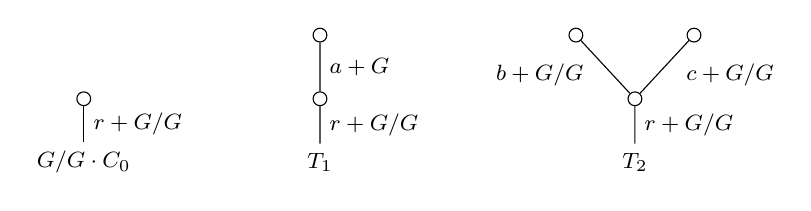
\begin{tikzpicture}[grow=up,auto,level distance=2.3em,every node/.style = {font=\footnotesize},dummy/.style={circle,draw,inner sep=0pt,minimum size=1.75mm}]
	\node at (0,0) {$G/G \cdot C_0$}
		child{
			node [dummy] {}
		edge from parent node [swap] {$r+G/G$}};
	\node at (3,0) {$T_1$}
		child{node [dummy] {}
			child{node [dummy] {}
			edge from parent node [swap] {$a+G$}}
		edge from parent node [swap] {$r+G/G$}};
	\node at (7,0) {$T_2$}
		child{node [dummy] {}
			child{node [dummy] {}
			edge from parent node [swap,near end] {$c+G/G$}}
			child{node [dummy] {}
			edge from parent node [near end] {$b+G/G$}}
		edge from parent node [swap] {$r+G/G$}};
\end{tikzpicture}
\]
However, when pulling these points back to the $G$-free stump corolla $G \cdot C_0$ one obtains the same point in 
$\mathbb F_G \iota_{\**} Y(G \cdot C_0)$,
%$^{\Gamma} = \iota_{\**} \iota^{\**} \mathbb F_G \iota_{\**} Y(G/G \cdot C_0)$
namely that encoded by the $G$-tree $T$ below.
\[
\begin{tikzpicture}[grow=up,auto,level distance=2.3em,every node/.style = {font=\footnotesize},dummy/.style={circle,draw,inner sep=0pt,minimum size=1.75mm}]
	\node at (0,0) {$G \cdot C_0$}
		child{
			node [dummy] {}
		edge from parent node [swap] {$r+G$}};
	\node at (5,0) {$T$}
		child{node [dummy] {}
			child{node [dummy] {}
			edge from parent node [swap,near end] {$c+G$}}
			child{node [dummy] {}
			edge from parent node [near end] {$b+G$}}
		edge from parent node [swap] {$r+G$}};
\end{tikzpicture}
\]
Moreover, it is not hard to modify the example above to produce similar examples when evaluating $\mathbb{F}_GY$ at non-empty corollas. 

However, such counter-examples all require the use of trees with stumps. Indeed, it can be shown that (\ref{KEYNONISO EQ})
is an isomorphism whenever evaluated at a $Y$ such that $Y(C_0)=\emptyset$.
\end{remark}


\renewcommand{\F}{\mathcal{F}}

\subsection{Indexing systems and partial genuine operads}
\label{INDEXING_SECTION}

As discussed preceding Theorem \ref{MAINEXIST2 THM},
the Elmendorf-Piacenza equivalence
(\ref{COFADJINT EQ}) has analogues
\[
\begin{tikzcd}[column sep =4em,row sep=0.3em]
	\mathsf{Top}^{\mathsf{O}_{\mathcal{F}}^{op}}
	\ar[shift left=1]{r}{\iota^{\**}} 
&
	\mathsf{Top}_{\mathcal{F}}^G
	\ar[shift left=1]{l}{\iota_{\**}}
\end{tikzcd}
\]
for each family $\mathcal{F}$ of subgroups of $G$.
Here $\mathsf{O}_\mathcal{F} \hookrightarrow \mathsf{O}_G$ consists of those $G/H$ such that $H \in \mathcal{F}$ 
and thus the objects of
$\mathsf{Top}^{\mathsf{O}_{\mathcal{F}}^{op}}$
are partial coefficient systems.
These specialized equivalences provide an alternative approach to universal 
$E \mathcal{F}$-spaces: rather than cofibrantly replacing the object
$\delta_{\mathcal{F}} \in \mathsf{Top}^{\mathsf{O}_G^{op}}$
as in the introduction,
one builds an $E \mathcal{F}$-space by
$\iota^{\**}(C \**) = (C *) (G)$
where now $\** \in \mathsf{Top}^{\mathsf{O}_{\mathcal{F}}^{op}}$
is the terminal object and $C$ the cofibrant replacement in $\mathsf{Top}^{\mathsf{O}_{\mathcal{F}}^{op}}$.

In keeping with the motivation that the Blumberg-Hill $N \mathcal{F}$ operads are the operadic analogues of universal $E \mathcal{F}$ spaces,
we will now show that the closure conditions for 
indexing systems
identified in \cite[Def. 3.22]{BH15}
are (almost exactly) the necessary conditions to define categories 
$\mathsf{Op}_{\mathcal{F}}$
of partial genuine equivariant operads.

We start by recalling that 
in the classic setting
$\mathcal{F}$ is a family of subgroups of $G$
if and only if the associated subcategory 
$\mathsf{O}_{\mathcal{F}} \hookrightarrow
\mathsf{O}_G$ is a sieve, defined as follows.


\begin{definition}
	A \textit{sieve} of a category $\mathcal{D}$
	is a subcategory $\mathcal{S}$ such that
	for any arrow $f \colon d \to s$ in $\mathcal{D}$ with 
	$s \in \mathcal{S}$ then both $d$ and $f$ are also in $\mathcal{S}$. 
	In particular, sieves are full subcategories.
\end{definition}


\begin{definition}\label{FAMILY_COROLLAS_DEF}
      We call a sieve
      %A \textit{family} of $G$-corollas is a sieve
      $\Sigma_{\mathcal{F}} \hookrightarrow \Sigma_G$
      a \textit{family of $G$-corollas}.
\end{definition}

\begin{remark}\label{FAMILY_COROLLAS_REM}
A family of $G$-corollas $\Sigma_{\mathcal{F}}$
can equivalently be encoded by
a collection $\F = \set{\F_n}_{n \geq 0}$ of 
families $\mathcal F_n$ of \textit{graph subgroups} of $G \times \Sigma_n$, so that there is an equivalence of categories
$\Sigma_\F \simeq \coprod \mathsf{O}_{\F_n}$ (see Lemma \ref{FAMILY_COROLLAS_LEM}).
	As such, we abuse notation and abbreviate either set of data as $\F$. 
\end{remark}

Writing 
$\upgamma \colon 
\Sigma_{\mathcal{F}}
\hookrightarrow
\Sigma_G$
for the inclusion and 
$\mathsf{Sym}_{\mathcal{F}}(\mathcal{V}) = 
\mathcal{V}^{\Sigma_{\mathcal{F}}^{op}}$,
we thus have a pair of adjunctions
\begin{equation}\label{F_TWOADJOINTS_EQ}
	\begin{tikzcd}[column sep =5em]
		\mathsf{Sym}_\F(\mathcal{V})
		\arrow[r, bend left, "\upgamma_{!}"]
		\arrow[r, bend right, "\upgamma_{\**}"']
	&
		\mathsf{Sym}_{G}(\mathcal{V}) 
		\arrow[l, "\upgamma^{\**}"] 
	\end{tikzcd}
\end{equation}
Our focus will be on the $(\upgamma_!,\upgamma^{\**})$ adjunction.
The requirement that $\Sigma_{\mathcal{F}}$ be a sieve then implies that $\upgamma_!$ simply extends presheaves by the initial object 
$\emptyset \in \mathcal{V}$,
so that $\gamma_!$ identifies 
$\mathsf{Sym}_{\mathcal{F}}(\mathcal{V})$
with a (coreflexive) subcategory of 
$\mathsf{Sym}_G(\mathcal{V})$.
One may then ask for conditions on the family 
of corollas $\mathcal{F}$ such that 
the genuine operad monad $\mathbb{F}_G$
preserves this subcategory.
% and, as it turns out,
The answer is almost exactly given by the Blumberg-Hill indexing systems.


\begin{definition}\label{FTREE DEF}
Let $\mathcal{F}$ be a family of $G$-corollas.

We say that a $G$-tree $T$ is a \textit{$\mathcal{F}$-tree}
if all of its $G$-vertices $T_{v}$, $v \in V_G(T)$ are in 
$\Sigma_{\mathcal{F}}$.
We denote by 
$\Omega_\F \hookrightarrow \Omega_G$,
$\Omega_\F^0 \hookrightarrow \Omega_G^0$
the full subcategories spanned by the $\F$-trees.
\end{definition}


\begin{remark}\label{VACUOUSNESS REM}
	By vacuousness the stick $G$-trees
	$(G/H) \cdot \eta = (\eta)_{G/H}$ are always $\mathcal{F}$-trees.
\end{remark}

%The primary purpose of the notion of $\mathcal{F}$-tree is to classify notions of ``partial genuine operads''.

%Now, given a family $\mathcal{F}$ of $G$-corollas and writing 
%$\mathsf{Sym}_{\mathcal{F}}(\mathcal{V}) = %\mathcal{V}^{\Sigma_{\mathcal{F}}^{op}}$ 
%for the partial $G$-symmetric sequences determined by $\mathcal{F}$, one may then ask under which conditions the construction of the monad
%$\mathbb{F}_G$ on $\mathsf{Sym}_{G}(\mathcal{V})$
%of \S \ref{FGMON SEC}
%can be adapted to build a monad
%$\mathbb{F}_{\mathcal{F}}$ on 
%$\mathsf{Sym}_{\mathcal{F}}(\mathcal{V})$.

%Writing $\Omega_{\mathcal{F}}^0 \hookrightarrow \Omega_{G}^0$ for the full subcategory of $\mathcal{F}-$trees and quotients, 
%this amounts to asking whether the leaf-root and vertex functors of \S \ref{LRVERT SEC} restrict to the $\mathcal{F}$ context. That the vertex functor restricts to a functor
%$V_G \colon \Omega_{\mathcal{F}}^0 \to \Fin \wr \Sigma_{\mathcal{F}}$ is in fact tautological: indeed,
%$\Omega_{\mathcal{F}}$ can be defined to be the pre-image 
%$(V_{G})^{-1}(\Fin \wr \Sigma_{\mathcal{F}})$.
%Compatibility with the leaf-root functor, however, 
%requires an additional closure condition on $\mathcal{F}$,
%which we now formally introduce.


\begin{definition}\label{INDEXSYS DEF}
	A family $\mathcal{F}$ of $G$-corollas is called a 
	\textit{weak indexing system}
	if for any $\mathcal{F}$-tree $T \in \Omega_{\mathcal{F}}^0$ we have 
	$\mathsf{lr}(T) \in \Sigma_{\mathcal{F}}$;
        that is, if the leaf-root functor restricts to a functor
	$\mathsf{lr} \colon \Omega_{\mathcal{F}}^0 \to \Sigma_{\mathcal{F}}$.
Moreover, $\mathcal{F}$ is called simply an \textit{indexing system} if all trivial corollas 
$(G/H)\cdot C_n = (C_n)_{G/H}$ are in $\Sigma_{\mathcal{F}}$.
\end{definition}


\begin{remark}
	In light of Remark \ref{VACUOUSNESS REM} any weak indexing system must contain the $1$-corollas $(G/H) \cdot C_1 \simeq (C_1)_{G/H}$ for all $H\leq G$.
\end{remark}

\begin{remark}
The notion of indexing system
was first introduced in \cite[Def. 3.22]{BH15}, though packaged quite differently.
Moreover, a third definition of (weak) indexing systems as certain sieves 
$\Omega_{\mathcal{F}} \hookrightarrow \Omega_G$
was presented by the second author in \cite[\S 9]{Pe17}. The equivalence between the definitions in \cite{BH15} and \cite{Pe17} is addressed in 
\cite[Rmk. 9.7]{Pe17}, hence here we address only the easier equivalence between Definition \ref{INDEXSYS DEF} and the sieve definition in \cite[\S 9]{Pe17}.

The existence of canonical maps 
$\mathsf{lr}(T) \to T$ shows that the sieve condition
implies the $\mathsf{lr}$ condition
in Definition \ref{INDEXSYS DEF}. 
Conversely, as discussed immediately preceding \cite[Def. 9.5]{Pe17}, the sieve condition needs only be checked for inner faces and degeneracies, i.e. tall maps, and thus follows from Definition \ref{INDEXSYS DEF} since the subcategory 
$\Omega_{\mathcal{F}}^1 \hookrightarrow \Omega^1_G$ 
of planar tall strings between $\mathcal{F}$-trees
matches the pullback of
$\Omega_{\mathcal{F}}^0 \to
\Fin \wr \Sigma_{\mathcal{F}} \leftarrow 
\Fin \wr \Omega_{\mathcal{F}}^0
$.
\end{remark}


The connection between weak indexing systems and $\mathbb{F}_G$ is given by the following,
which generalizes 
Proposition \ref{MONAD_COMPARISON_PROP}.


\begin{proposition}\label{F_MONAD_COMPARISON_PROP}
	Let $\F$ be a weak indexing system. Then:
	\begin{itemize}
	\item[(i)] the map 
		$\upgamma^{\**} \mathbb{F}_G
		\xrightarrow{\eta_{\**}}
		\upgamma^{\**} \mathbb{F}_G \upgamma_{\**} \upgamma^{\**}$
		is an isomorphism,
		and thus (cf. Prop. \ref{MONADADJ PROP})
		$\upgamma^{\**} \mathbb{F}_G \upgamma_{\**}$
		is a monad;
	\item[(ii)] the map
		$\upgamma^{\**} \mathbb{F}_G \upgamma_{!}
		\xrightarrow{\beta}
		\upgamma^{\**} \mathbb{F}_G \upgamma_{\**}$ is an isomorphism of monads;
	\item[(iii)] the map
		$\upgamma_{!}\upgamma^{\**} \mathbb{F}_G \upgamma_{!}
		\xrightarrow{\epsilon_!}
		\mathbb{F}_G \upgamma_{!}$ is an isomorphism.
	\end{itemize}
\end{proposition}

\begin{proof}
	This follows just like the analogous parts of
	Proposition \ref{MONAD_COMPARISON_PROP} by
	replacing
	$\mathsf{lr}: \Omega_G^{0,\text{fr}} \to \Sigma_G^{\text{fr}}$
	with
	$\mathsf{lr}: \Omega_{\F}^0 \to \Sigma_{\F}$. 
	For (i), note that if $C \in \Sigma_{\mathcal{F}}$
	there is an identification between
	$C \downarrow_{\mathsf r} \Omega_G^0$
	and
	$C \downarrow_{\mathsf r} \Omega_{\F}^0$,
	so that $\mathbb{F}_G X (C)$
	only depends on the values of $X$ on $\Sigma_{\mathcal{F}}$.
	(ii) is immediate.	
	Lastly, (iii) follows 
	since if $C \nin \Sigma_{\mathcal{F}}$ then
	any tree in $C \downarrow_{\mathsf r} \Omega_G^0$ must contain at least one $G$-vertex not in $\Sigma_{\mathcal{F}}$,
	so that indeed $\mathbb{F}_G \upgamma_{!}Y(C)=\emptyset$.
%        Thus for $X\in \Sym_G(\V)$, $\upgamma^{\**} \mathbb{F}_G X$ is computed by the Kan extension of the following diagram,
%        \begin{equation}
%              \label{F_F_LAN_EQ}
%              \begin{tikzcd}
%                    \Omega_{\F}^{0} \ar{d} \ar{r} &
%                    \Fin \wr \Sigma_{\F} \ar{r}{\Fin \wr X} &
%                    \Fin \wr \mathcal{V}^{op} \ar{r} &
%                    \mathcal{V}^{op}
%                    \\
%                    \Sigma_{\F}
%              \end{tikzcd}
%        \end{equation}
%        and the result follows since $X \to \upgamma_{\**} \upgamma^{\**} X$ is a isomorphism when restricted to $\Sigma_{\F}$. 
%        
%        The remaining results follow from similarly analogous proofs.
\end{proof}

\begin{notation}
We write 
$\mathbb{F}_{\mathcal{F}} = \upgamma^{\**} \mathbb{F}_G \upgamma_!$ for the induced monad
on
$\mathsf{Sym}_{\mathcal{F}}(\mathcal{V})$,
and $\mathsf{Op}_{\mathcal{F}}(\mathcal{V})$
for the corresponding categories of algebras.
\end{notation}

\begin{corollary}\label{TWOADJOINTSOPF COR}
The adjunctions (\ref{F_TWOADJOINTS_EQ}) lift to adjunctions
\begin{equation}\label{TWOADJOINTSOPF EQ}
	\begin{tikzcd}[column sep =5em]
		\mathsf{Op}_\F(\mathcal{V})
			\arrow[r, bend left, "\upgamma_{!}"]
			\arrow[r, bend right, "\upgamma_{\**}"']
		&
		\mathsf{Op}_{G}(\mathcal{V})
		\arrow[l, "\upgamma^{\**}"]
	\end{tikzcd}
\end{equation}
\end{corollary}

\begin{remark}\label{WINDEX_GAMMA_REM}
Part (iii) of Proposition \ref{F_MONAD_COMPARISON_PROP}
states that if $\mathcal{F}$ is a weak indexing system then $\mathbb{F}_G$ essentially preserves the image of $\upgamma_!$ (moreover, the converse is easily seen to also hold).
As such, we will sometimes find it conceptually convenient
to regard $\mathbb{F}_{\mathcal{F}}$ as
``restricting $\mathbb{F}_G$''.
\end{remark}

%This mimics one possible interpretation of the main results from \cite[\S 4]{BH15},
%where indexing systems provide the closure conditions necessary to ensure that 
%composite operations $f(g_1,\ldots,g_n)$ have $\F$-admissible isotropy whenever the $x$ and $y_i$ do;
%that is, the operadic structure ``restricts'' to indexing systems.
%
%This view of Part (iii) also indicates a reason why we chose to define $\mathbb F_\F$ in this way, as opposed to building an entirely new operad given by left Kan extensions as in (\ref{F_F_LAN_EQ}) and repeating the arguments from \S \ref{FGMON SEC} mutatis mutandis.
        
\begin{remark}        
	The free corollas of \S	\ref{COMPARISON_REGULAR_SECTION}
	form a weak indexing system
	$\Sigma_G^{\text{fr}} = \Sigma_{\F_{\text{fr}}}$
	and, moreover, there is an equivalence of categories
	$\Op^G \simeq \Op_{\F_{\text{fr}}}$,
	so that Corollary \ref{TWOADJOINTSOP_COR}
%	(\ref{TWOADJOINTSOP EQ})
	is a particular case of 
	Corollary \ref{TWOADJOINTSOPF COR}.
	However, while our discussion of 
	Corollary \ref{TWOADJOINTSOP_COR}
	focuses on the $(\iota^{\**},\iota_{\**})$-adjunction, due to the fact that the intended model structures on $\mathsf{Op}^G(\mathcal{V})$ in
	Theorem \ref{MAINEXIST1 THM} are defined via fixed point conditions, 
	our discussion of 
	Corollary \ref{TWOADJOINTSOPF COR}
%	(\ref{TWOADJOINTSOPF EQ})
	focuses on the $(\iota_{!},\iota^{\**})$-adjunction, due to the model structures in 
	Theorem \ref{MAINEXIST2 THM} being projective.
\end{remark}

\begin{remark}\label{COMPADJ REM}
	In most cases, the rightmost $(\iota^{\**},\iota_{\**})$-adjunction appearing in Theorem \ref{MAINQUILLENEQUIV THM}
	is induced by an inclusion 
	$\iota \colon \Sigma_G^{\text{fr}} \hookrightarrow \Sigma_{\mathcal{F}}$.
	However, it is possible for  
	$\Sigma_G^{\text{fr}} \nsubset \Sigma_{\mathcal{F}}$ (the most interesting case being that of
	$\Sigma_{\mathcal F} = \Sigma_{G}^{\geq 1}$
	the corollas of arity $\geq 1$, which model non-unital operads).
	In these cases (and compatibly with the 
	$\Sigma_G^{\text{fr}} \hookrightarrow \Sigma_{\mathcal{F}}$ case), we instead use the composite adjunction
\begin{equation}\label{COMPADJ EQ}
\begin{tikzcd}[column sep =5em]
	\mathsf{Op}_\F(\mathcal{V})
	\ar[shift left=1.5]{r}{\upgamma_!} 
&
	\mathsf{Op}_{G}(\mathcal{V}) 
	\arrow[l, shift left=1.5, "\upgamma^{\**}"] 
	\arrow[r, shift left=1.5,swap,"\iota^{\**}"']
&
	\mathsf{Op}^G(\mathcal{V})
	\ar[shift left=1.5]{l}{\iota_{\**}}
\end{tikzcd}
\end{equation}
Note that the right adjoint 
$\gamma^{\**} \iota_{\**}$
is still defined by computing fixed points while the 
left adjoint
$\iota^{\**}\gamma_!$
is still essentially a forgetful functor, with those levels not present in $\mathcal{F}$ declared to be $\emptyset$.

In practice, however, the use of the composite adjunction
(\ref{COMPADJ EQ})
is fairly benign, requiring only minor
adjustments to the notation of the proofs in 
\S \ref{MAINTHM_PROOF_SECTION}.
\end{remark}

%\begin{remark}
%       A minor warning:
%       if $\Sigma_\F$ does not contain the free $G$-tree $G \cdot C_n$ for some $n \geq 0$
%        (which is possible even for indexing systems),
%        then the composite $\upgamma^{\**} \iota_{\**}$ is no longer injective on objects out of $\Sym^G_\F(\V)$. 
%        and hence this adjunction is no longer reflective.
%        
%        Instead, we will see that it is reflective only on \textit{cofibrant} objects in $\Sym^G_\F(\V)$. 
%\end{remark}



%%%%%%%%%%%%%%%%%%%%%%%%%%%%%%%%

\renewcommand{\F}{\mathbb{F}}

\section{Free extensions and the existence of model structures}
\label{FREE_EXTENSIONS_SECTION}

In order to prove all of our main theorems
we will need to homotopically analyze free extensions 
of genuine equivariant operads,
i.e. pushouts of the form
\begin{equation}
  \label{FREE_FG_EXT_EQ}
  \begin{tikzcd}
    \mathbb{F}_G X \ar{r} \ar{d}[swap]{\mathbb{F}_G u} & \mathcal{P} \ar{d}
    \\
    \mathbb{F}_G Y \ar{r} & \mathcal{P}[u]
  \end{tikzcd}
\end{equation}
in the category $\mathsf{Op}_G(\mathcal{V})$.
As is common in the literature (e.g. \cite{SS00, Spi01, BM03, Whi14, Pe16}),
the key technical ingredient will be the identification of a suitable filtration
\begin{equation}\label{FILTR EQ}
	\mathcal{P}=\mathcal{P}_0 \to 
	\mathcal{P}_1 \to \mathcal{P}_2 \to
	\cdots \to \mathcal{P}_{\infty}=\mathcal{P}[u]
\end{equation}
of the map $\mathcal{P} \to \mathcal{P}[u]$
in the underlying category $\mathsf{Sym}_G(\mathcal{V})$.
To explain how this filtration is obtained,
%and abbreviating 
%$\mathbb{F}_G$ as $\mathbb{F}$,
note first that $\mathcal{P}[u]$ is given by a coequalizer
\begin{equation}\label{REFLCOEQ EQ}
\begin{tikzcd}
	\mathcal{P} \mathbin{\check{\amalg}}
	\mathbb{F}_G X \mathbin{\check{\amalg}} \mathbb{F}_G Y
	\ar[shift right=4pt]{r} \ar[shift right=-4pt]{r}
&
	\mathcal{P} \mathbin{\check{\amalg}} \mathbb{F}_G Y 
	\ar[dashed]{l}
\end{tikzcd}
\end{equation}
where $\check{\amalg}$ denotes the algebraic coproduct, 
i.e. the coproduct in $\mathsf{Op}_G(\mathcal{V})$, and, a priori,
the coequalizer is also calculated in $\mathsf{Op}_G(\mathcal{V})$. However, (\ref{REFLCOEQ EQ}) is a so called \textit{reflexive coequalizer}, meaning that the maps being coequalized have a common section,
and standard arguments\footnote{
For example, by the proof of 
\cite[Prop. 3.27]{Ha09}
it suffices to check that 
$\mathbb{F}_G$ preserves reflexive coequalizers.
This follows from (\ref{FGXDEF EQ}) and the fact that if $\otimes$ preserves colimits in each variable then
it preserves reflexive coequalizers.}
 show that 
it is hence also an underlying coequalizer in 
$\mathsf{Sym}_G(\mathcal{V})$.

In practice, we will need to enlarge 
(\ref{REFLCOEQ EQ}) somewhat.
Firstly, note that (\ref{REFLCOEQ EQ})
corresponds to the two bottom levels of the bar construction
$B_l(\mathcal{P}, \mathbb{F}_G X, \mathbb{F}_G Y)=
\mathcal{P} \mathbin{\check{\amalg}}
(\mathbb{F}_G X)^{\check{\amalg} l} 
\mathbin{\check{\amalg}} \mathbb{F}_G Y$,
whose colimit (over $\Delta^{op}$) is again $\mathcal{P}[u]$.
For technical reasons, we prefer the double bar construction
\footnote{
More formally,
$B_{\bullet}(\mathcal{P}, \mathbb{F} X, \mathbb{F} X, \mathbb{F} X, \mathbb{F} Y)$
is the diagonal
of the iterated bar construction
$B^{op}_{\bullet}\left(\mathcal{P}, \mathbb{F} X, 
B_{\bullet}(\mathbb{F} X, \mathbb{F} X, \mathbb{F} Y)\right)$,
where the $op$ indicates that in the outer bar construction we reverse the order of the simplicial operators.
}
(where to increase readability, we 
abbreviate $\mathbb{F}_G$ as $\mathbb{F}$)
\begin{equation}\label{DOUBAR EQ}
	B_l(\mathcal{P}, \mathbb{F} X, \mathbb{F} X, \mathbb{F} X, \mathbb{F} Y)
=
	\mathcal{P} \mathbin{\check{\amalg}}
	(\mathbb{F} X)^{\check{\amalg} l} 
	\mathbin{\check{\amalg}}
	\mathbb{F} X
	\mathbin{\check{\amalg}}
	(\mathbb{F} X)^{\check{\amalg} l} 
	\mathbin{\check{\amalg}} \mathbb{F} Y
=
	\mathcal{P} \mathbin{\check{\amalg}}
	(\mathbb{F} X)^{\check{\amalg} 2l+1} 
	\mathbin{\check{\amalg}} \mathbb{F} Y.
\end{equation}
To actually describe the individual levels  of
(\ref{DOUBAR EQ}) one further resolves $\mathcal{P}$
so as to obtain the bisimplicial object
(we again abbreviate $\mathbb{F}_G$ as $\mathbb{F}$)
\begin{equation}\label{FURRES EQ}
	B_l(\mathbb{F}^{n+1}\mathcal{P}, \mathbb{F} X, \mathbb{F} X, \mathbb{F} X, \mathbb{F} Y)
=
	\mathbb{F}^{n+1}\mathcal{P} \mathbin{\check{\amalg}}
	(\mathbb{F} X)^{\check{\amalg} 2l+1} 
	\mathbin{\check{\amalg}} \mathbb{F} Y
\simeq
	\mathbb{F}\left(
		\mathbb{F}^{n} \mathcal{P} \amalg
		X^{\amalg 2l+1} \amalg Y
	\right),
\end{equation}
where $\amalg$ denotes the coproduct in $\mathsf{Sym}_G(\mathcal{V})$.
As in Remark \ref{REPACKAGERES REM}, each level of 
(\ref{FURRES EQ})
can then be described as 
\begin{equation}\label{LANLEVELFOR EQ}
 \mathsf{Lan} N (N^{n} \iota \mathcal{P} 
\amalg \iota X^{\amalg 2l+1} \amalg \iota Y)
=
\mathsf{Lan} N^{(\mathcal P, X, Y)}_{n,l},
\end{equation}
for $N$ the span monad (cf. Definition \ref{WSPAN_MONAD_DEFINITION}) and $\amalg$ now the coproduct of spans.
In particular, each level of 
(\ref{FURRES EQ})
is thus a left Kan extension over some category
$\Omega_G^{n,\lambda_l}$, which we explicitly identify in 
\S \ref{LABELSTRI SEC}, giving the first identification below.
\begin{equation}\label{EXTTREEFOR EQ}
	\mathcal{P} \mathbin{\check{\coprod}}_{\mathbb{F}_G X} \mathbb{F}_G Y 
\simeq 
	\colim_{(\Delta \times \Delta)^{op}}
	\left(
	\mathsf{Lan}_{\left( \Omega_{G}^{n,\lambda_l} \to \Sigma_G \right)^{op}}
	N_{n,l}^{(\mathcal{P},X,Y)}
	\right)
\simeq 
	\mathsf{Lan}_{\left( \Omega_{G}^{e} \to \Sigma_G \right)^{op}}
	\tilde{N}^{(\mathcal{P},X,Y)}
\end{equation}
The second identification, 
which reduces the calculation to a single left Kan extension, is an instance of 
Proposition \ref{RANTRANS PROP}, 
a result whose proof is straightforward but lengthy, 
and thus postponed to the appendix.
The category $\Omega_G^e$ of \textit{extension trees}
appearing on the right side
is obtained as a categorical realization
$\Omega_G^e = |\Omega_{G}^{n,\lambda_l}|$,
which we explicitly describe and analyze in 
\S \ref{EXTTREE SEC}.
In particular, we identify a smaller and more convenient
subcategory 
$\widehat{\Omega}_G^e \hookrightarrow \Omega_G^e$
that is suitably initial,
so that $\Omega_G^e$ can be replaced with $\widehat{\Omega}_G^e$
in (\ref{EXTTREEFOR EQ}).

The desired filtration (\ref{FILTR EQ})
then follows from a filtration of the 
category $\widehat{\Omega}_G^e$ itself,
and this discussion is the subject of
\S \ref{FILTRATION_SECTION}.

Lastly, \S \ref{MAINEXIST SEC} concludes this section
by using these filtrations to prove 
Theorems \ref{MAINEXIST1 THM} and \ref{MAINEXIST2 THM}.

%This filtration will allow for a homotopical study of these free extensions, which combined with the transfer principle of Kan \cite[Thm. 11.3.2]{Hi03} will allow us to prove Theorems \ref{MAINEXIST1 THM} and \ref{MAINEXIST2 THM}, endowing the categories of equivariant operads with multiple model structures, in \S \ref{MAINEXIST SEC}.


\subsection{Labeled planar strings}\label{LABELSTRI SEC}


In this section, we explicitly identify the categories underlying the left Kan extensions in (\ref{LANLEVELFOR EQ}).


In the notation 
of Remark \ref{PRECOMPPOSTCOMP REM},
letting 
$\langle \langle l 
\rangle \rangle = 
\{-\infty,-l,\cdots, -1, 0, 1, \cdots, l, \infty\}$ and writing
$\lambda_{l}$ for the partition
$\lambda_{l,a} = \{-\infty\}$,
$\lambda_{l,i} = 
\langle \langle l \rangle \rangle - \{-\infty\}$,
(\ref{LANLEVELFOR EQ})
can be repackaged as an instance of the functor
$\mathsf{Lan} \circ N \circ \coprod \circ (N^{\times \lambda_l})^{\circ n}\circ \iota^{\times \langle \langle l \rangle \rangle}$.
Our goal is thus to understand 
the underlying categories of the spans in the image of the functor
$N \circ \coprod \circ (N^{\times \lambda_l})^{\circ n}$,
though we will find it preferable and no harder to tackle the more general case of the functors 
$N^{s+1} \circ \coprod \circ (N^{\times \lambda})^{\circ n-s}$.

\begin{definition}\label{LABMAP DEF}
A \textit{$l$-node labeled $G$-tree} (or just \textit{$l$-labeled $G$-tree}) is a pair $(T,V_G(T) \to \{1,\cdots,l\})$ with $T \in \Omega_G$, which we think of as a $G$-tree together with $G$-vertices labels in $1,\cdots,l$.

Further, a tall map $\varphi \colon T \to S$ between $l$-labeled trees is called a \textit{label map} if, for each $G$-vertex $v_{G e}$ of $T$ with label $j$, all vertices of the subtree $S_{v_{G e}}$ (cf. \eqref{TVGE DEF}) are labeled by $j$.

Lastly, given a subset $J\subset \underline{l}$, a planar label map $\varphi \colon T \to S$ is said to be $J$-inert if for every $G$-vertex $v_{G e}$ of $T$ with label $j \in J$, we have $S_{v_{Ge}} = T_{v_{Ge}}$.
\end{definition}


\begin{example}\label{LABELEDTREES EX}
Consider the $2$-labeled trees below (for $G=\**$ the trivial group), with black nodes ($\bullet$) denoting labels by the number $1$ and white nodes ($\circ$) labels by the number $2$.
The planar map $\varphi$ (sending $a_i\mapsto a$, 
$b \mapsto b$, $c \mapsto c$, $d \mapsto d$, $e \mapsto e$) is a label map which is $\{1\}$-inert.
\[
	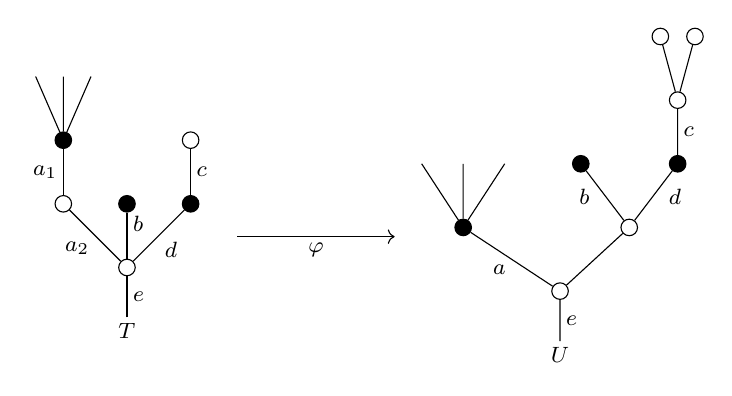
\begin{tikzpicture}[grow=up,auto,level distance=2.1em,
	every node/.style = {font=\footnotesize,inner sep=2pt},
	dummy/.style={circle,draw,inner sep=0pt,
	minimum size=2.1mm}]
	\begin{scope}[level distance=2.3em]
	\tikzstyle{level 2}=[sibling distance=3.5em]%
	\tikzstyle{level 3}=[sibling distance=2.25em]%
	\tikzstyle{level 4}=[sibling distance=1.25em]%
	\tikzstyle{level 5}=[sibling distance=1.25em]%
		\node at (5.5,0) {$U$}
			child{node [dummy] {}
				child[sibling distance =5em]{node [dummy] {}
					child[sibling distance =3.5em]{node [dummy,fill=black] {}
						child{node [dummy] {}
							child{node [dummy] {}}
							child{node [dummy] {}}
						edge from parent node [swap] {$c$}}
					edge from parent node [swap, near end] {$d$}}
					child[sibling distance =3.5em]{node [dummy,fill=black] {}
					edge from parent node [near end] {$b$}}
				}
				child[sibling distance =7em]{node [dummy,fill=black] {}
					child[sibling distance =1.5em]
					child[sibling distance =1.5em]
					child[sibling distance =1.5em]
				edge from parent node {$a$}}
			edge from parent node [swap] {$e$}};
	\end{scope}
	\begin{scope}[level distance=2.3em]
	\tikzstyle{level 2}=[sibling distance=2.3em]%
	\tikzstyle{level 4}=[sibling distance=1em]%
		\node at (0,0.3) {$T$}
			child{node [dummy] {}
				child{node [dummy,fill=black] {}
					child{node [dummy] {}
					edge from parent node [swap] {$c$}}	
				edge from parent node [swap] {$d$}}
				child{node [dummy,fill=black] {}
				edge from parent node [near end,swap] {$b$}}
				child{node [dummy] {}
					child{node [dummy,fill=black] {}
						child
						child
						child
					edge from parent node {$a_1$}}
				edge from parent node {$a_2$}}
			edge from parent node [swap] {$e$}};
	\end{scope}
	\draw [->] (1.4,1.5) -- node[swap] {$\varphi$} (3.4,1.5);
	\end{tikzpicture}
\]
\end{example}


\begin{definition}
Let $-1 \leq s \leq n$ and 
$\lambda = \lambda_a \amalg \lambda_i$
a partition of $\{1,2,\cdots,l\}$.

We define $\Omega_{G}^{n,s,\lambda}$ to have as objects $n$-planar strings (where $T_{-1} = \mathsf{lr}(T_0)$ as in (\ref{STRINGOBJALT EQ}))
\begin{equation}\label{NSTRINGLAB EQ}
	T_{-1} \xrightarrow{\varphi_0}
	T_0 \xrightarrow{\varphi_1}
	T_1 \xrightarrow{\varphi_2}
	\cdots \xrightarrow{\varphi_s}
	T_s \xrightarrow{\varphi_{s+1}}
	T_{s+1} \xrightarrow{\varphi_{s+2}}
	\cdots \xrightarrow{\varphi_n}
	T_{n}
\end{equation}
together with
$l$-labelings of $T_s, T_{s+1},\cdots, T_{n}$ such that the $\varphi_r,r>s$ are $\lambda_i$-inert label maps.

Arrows in $\Omega_{G}^{n,s,\lambda}$ are quotients of strings
$(\pi_r \colon T_r \to T'_r)$ such that 
$\pi_r, r\geq s$ are label maps.

Further, for any $s<0$ or $n<s'$ we write
\begin{equation}\label{EXTRACASES EQ}
	\Omega_{G}^{n,s,\lambda} = 
		\Omega_{G}^{n,-1,\lambda},
\qquad
	\Omega_{G}^{n,s',\lambda} = \Omega_{G}^{n}.
\end{equation}
\end{definition}

Intuitively, $\Omega_G^{n,s,\lambda}$ consists of strings that are labeled in the range $s \leq r \leq n$,
with the extra cases (\ref{EXTRACASES EQ}) interpreted by infinitely prepending and postpending copies of $T_{-1}$ and $T_n$ to (\ref{NSTRINGLAB EQ}).

The main case of interest is that of $s=0$, which we abbreviate as $\Omega_{G}^{n,\lambda} = \Omega_{G}^{n,0,\lambda}$,
with the remaining
$\Omega_{G}^{n,s,\lambda}$ playing an auxiliary role.
The $s=-1$ case also deserves special attention.

\begin{remark}
	For $s<0$ there are identifications 
\begin{equation}\label{OMEGANMINUSONE EQ}
	\Omega_{G}^{n,s,\lambda} = 
	\Omega_{G}^{n,-1,\lambda} \simeq
		\coprod_{\lambda_a} \Omega_{G}^{n} \amalg
		\coprod_{\lambda_i} \Sigma_G.
\end{equation}
Indeed, since $T_{-1}$ is a $G$-corolla, the label of its unique $G$-vertex determines all other labels.
\end{remark}

\begin{notation}
We will write $(\Omega_G^n)^{\times \lambda}$ to denote the $l$-tuple with 
$(\Omega_G^n)^{\times \lambda}_j = \Omega_G^n$ if 
$j \in \lambda_a$ and
$(\Omega_G^n)^{\times \lambda}_j = \Sigma_G$ if
$j \in \lambda_i$.
As such, (\ref{OMEGANMINUSONE EQ}) can be abbreviated as
$\Omega_{G}^{n,-1,\lambda} = \coprod (\Omega_G^n)^{\times \lambda}$.
\end{notation}

The $\Omega_G^{n,s,\lambda}$ categories are related by a number of obvious functors, which we now catalog.

Firstly, if $s \leq s'$ there are forgetful functors
\begin{equation}\label{NKNFGT EQ}
	\Omega_{G}^{n,s,\lambda} \to \Omega_{G}^{n,s',\lambda}
\end{equation}
and the simplicial operators
in Notation \ref{SIMPOPERATORS NOT}
generalize to operators (for $0 \leq i \leq n$, $-1\leq j \leq n$)
\begin{equation}\label{LABSTSIM EQ}
\begin{tikzcd}[row sep =0,column sep =1em]
	d_i \colon 
	\Omega_{G}^{n,s,\lambda} \ar{r} &
	\Omega_{G}^{n-1,s-1,\lambda} &
	i < s & & & &
	s_j \colon 
	\Omega_{G}^{n,s,\lambda} \ar{r} &
	\Omega_{G}^{n+1,s+1,\lambda} &
	j < s
\\
	d_i \colon 
	\Omega_{G}^{n,s,\lambda} \ar{r} &
	\Omega_{G}^{n-1,s,\lambda} &
	s \leq i & & & &
	s_j \colon 
	\Omega_{G}^{n,s,\lambda} \ar{r} &
	\Omega_{G}^{n+1,s,\lambda} &
	s \leq j
\end{tikzcd}
\end{equation}
which are compatible with the forgetful functors in the obvious way.

We will prefer to reorganize 
(\ref{NKNFGT EQ}) and (\ref{LABSTSIM EQ}) somewhat.
Defining functions 
$d_i \colon \mathbb{Z} \to \mathbb{Z}$
and 
$s_j \colon \mathbb{Z} \to \mathbb{Z}$
by
\begin{equation}\label{INTERMAPDEF EQ}
d_i(s) = 
	\begin{cases}
		s-1, & i<s
	\\
		s, & s \leq i
	\end{cases}
\qquad
s_j(s) = 
	\begin{cases}
		s+1, & j<s
	\\
		s, & s \leq j
	\end{cases}
\end{equation}
(\ref{LABSTSIM EQ}) can be rewritten as maps
$
	d_i \colon 
	\Omega_{G}^{n,s,\lambda} \to
	\Omega_{G}^{n-1,d_i(s),\lambda}
$
and 
$
	s_j \colon 
	\Omega_{G}^{n,s,\lambda} \to
	\Omega_{G}^{n+1,s_j(s),\lambda}
$.
Therefore, we henceforth write simply
$\Omega_G^{n,\bullet,\lambda}$ to denote the string of categories $\Omega_G^{n,s,\lambda}$
and forgetful functors, and abbreviate (\ref{LABSTSIM EQ}) as
\[
\begin{tikzcd}[row sep =0,column sep =1em]
	d_i \colon 
	\Omega_{G}^{n,\bullet,\lambda} \ar{r} &
	\Omega_{G}^{n-1,\bullet,\lambda} & & & &
	s_j \colon 
	\Omega_{G}^{n,\bullet,\lambda} \ar{r} &
	\Omega_{G}^{n+1,\bullet,\lambda}
\end{tikzcd}
\]

\begin{remark}\label{ORDLABEL REM}
Considering the ordered sets 
$\langle n \rangle =\{0 < 1 < \cdots < n < +\infty\}$, the formulas (\ref{INTERMAPDEF EQ}) 
define functions
$d_i \colon \langle n \rangle  \to \langle n-1 \rangle$
,
$s_j \colon \langle n \rangle  \to \langle n+1 \rangle$
which preserve $0$ and $+\infty$, except for 
$s_{-1}$ which preserves only
$+\infty$.
This recovers the description of $\Delta^{op}$
as the category of intervals (i.e. ordered finite sets with a minimum and maximum and maps preserving them).
\end{remark}


Next, the vertex functors $V_G^k$ of
(\ref{VGNISO EQ}) generalize to functors
$
	V_G^k \colon
	\Omega_G^{n,s,\lambda} \to
	\Fin_s \wr \Omega_G^{n-k-1,s-k-1,\lambda}
$
given by the same formula
\[
	(T_{k,v_{G e}}\to \cdots \to T_{n,v_{G e}})_{v_{G e} \in V_G(T_k)},
\]
as in (\ref{VGNISO EQ}),
except with $T_{m,v_{G e}}$ for $k \leq m \leq n$ inheriting the node labels from $T_m$ (if any).

The diagrams in (\ref{PIIDEFDI EQ})
for $i<k$ and $i>k$ now generalize to diagrams
\begin{equation}\label{PIIDEFDILAB EQ}
\begin{tikzcd}[row sep=1.7em,column sep = 3em]
	\Omega_{G}^{n,\bullet,\lambda} \ar{d}[swap]{d_{i}} \ar{r}{V_G^k} &
	|[alias=F1]|
	\Fin_s \wr \Omega_{G}^{n-k-1,\bullet,\lambda}
	\ar[equal]{d} 
&
	\Omega_{G}^{n,\bullet,\lambda} \ar{d}[swap]{d_{i}} \ar{r}{V_G^k} &
	\Fin_s \wr \Omega_{G}^{n-k-1,\bullet,\lambda}
	\ar{d}{d_{i-k-1}} 
\\
	|[alias=G2]|
	\Omega_{G}^{n-1,\bullet,\lambda} \ar{r}[swap]{V_G^{k-1}}&
	\Fin_s \wr \Omega_{G}^{n-k-1,\bullet,\lambda}  
&
	\Omega_{G}^{n-1,\bullet,\lambda} \ar{r}[swap]{V_G^{k}}&
	\Fin_s \wr \Omega_{G}^{n-k-2,\bullet,\lambda}  
\arrow[Leftrightarrow, from=F1, to=G2,shorten >=0.15cm,shorten <=0.15cm,"\pi_{i}"]
\end{tikzcd}
\end{equation}
while the diagrams in (\ref{PIIDEFDI2 EQ})
for $j<k$ and $j>k$ generalize to diagrams
\begin{equation}\label{PIIDEFDI2LAB EQ}
\begin{tikzcd}[row sep=1.7em,column sep = 3em]
	\Omega_{G}^{n,\bullet,\lambda} \ar{d}[swap]{s_{j}} \ar{r}{V_G^k} &
	|[alias=F1]|
	\Fin_s \wr \Omega_{G}^{n-k-1,\bullet,\lambda}
	\ar[equal]{d} 
&
	\Omega_{G}^{n,\bullet,\lambda} \ar{d}[swap]{s_{j}} \ar{r}{V_G^k} &
	\Fin_s \wr \Omega_{G}^{n-k-1,\bullet,\lambda}
	\ar{d}{s_{j-k-1}} 
\\
	|[alias=G2]|
	\Omega_{G}^{n+1,\bullet,\lambda} \ar{r}[swap]{V_G^{k+1}}&
	\Fin_s \wr \Omega_{G}^{n-k-1,\bullet, \lambda}  
&
	\Omega_{G}^{n+1,\bullet, \lambda} \ar{r}[swap]{V_G^{k}}&
	\Fin_s \wr \Omega_{G}^{n-k,\bullet,\lambda}  
\end{tikzcd}
\end{equation}
where we note that in all cases the $s$-index $\bullet$
varies according to (\ref{LABSTSIM EQ}).

Lastly, the $\Omega_G^{n,s,\lambda}$ are also functorial in $\lambda$. Explicitly, given 
$\alpha \colon \{1,\cdots,l\} \to \{1,\cdots,m\}$
and partitions such that 
$\lambda' \leq \alpha^{\**} \lambda$
one has forgetful functors
\begin{equation}\label{LAMBINC EQ}
	\Omega_G^{n,s,\lambda'}
\to
	\Omega_G^{n,s,\lambda}
\end{equation}
compatible with the forgetful functors (\ref{NKNFGT EQ}),
the simplicial operators $d_i$, $s_j$ and the isomorphisms
$\pi_i$.

\begin{remark}
	When $\alpha$ is the identity 
and $\lambda' \leq \lambda$ the forgetful functors in
(\ref{LAMBINC EQ}) are fully faithful inclusions.
	However, this is not the case for the  forgetful functors in (\ref{NKNFGT EQ}).
	Indeed, regarding the map $T \to U$ in
	Example \ref{LABELEDTREES EX}
	as an object in $\Omega_G^{1,0,\lambda}$
	for $\lambda = 
	\lambda_a \amalg \lambda_i = \{2\} \amalg \{1\}
	=\{\bullet\} \amalg \{\circ\}$,
	changing the label of $a_1 \leq a_2$ to a 
	$\bullet$-label produces a non isomorphic object
	$\bar{T} \to U$ of $\Omega_G^{1,0,\lambda}$
	that forgets to the same object of 
	$\Omega_G^{1,1,\lambda}$.
\end{remark}


We now extend Notation \ref{OMEGAGNA NOT}.

\begin{notation}
Let $(A_j)=(A_j \to \Sigma_G)_{1\leq j \leq l}$ be a $l$-tuple of categories over $\Sigma_G$.
We define 
$\Omega_{G}^{n,s,\lambda} \wr (A_j) $
as the pullback
\begin{equation}\label{OMEGAWRTUP EQ}
\begin{tikzcd}[row sep=1em]
	\Omega_{G}^{n,s,\lambda} \wr (A_j) \ar{r}{V_{G}^{n}} \ar{dd}& 
	\Fin \wr \coprod A_j \ar{d}
\\
	& \Fin \wr \coprod_l \Sigma_G \ar{d}
\\
	\Omega_{G}^{n,s,\lambda} \ar{r}[swap]{V_{G}^{n}} &
	\Fin \wr \Omega_G^{-1,s-n-1,\lambda}
\end{tikzcd}
\end{equation}
\end{notation}

\begin{remark}
To unpack (\ref{OMEGAWRTUP EQ}),
note first that by (\ref{EXTRACASES EQ}) $\Omega_G^{-1,r,\lambda}$ is simply either 
$\Sigma_G^{\amalg l}$ if $r<0$ or 
$\Sigma_G$ if $r \geq 0$,
while $\Omega_G^{n,s,\lambda} = \coprod (\Omega_{G}^{n})^{\times \lambda}$ if $s<0$.
We can thus break down
(\ref{OMEGAWRTUP EQ})
into the three cases
$s<0$, $0 \leq s \leq n$ and $n < s$,
depicted below.
\begin{equation}
\begin{tikzcd}[column sep =1.4em]
	\Omega_{G}^{n,s,\lambda} \wr (A_j) \ar{r}{V_{G}^{n}} \ar{d}& 
	\Fin \wr \coprod_j A_j \ar{d}
&
	\Omega_{G}^{n,s,\lambda} \wr (A_j) \ar{r}{V_{G}^{n}} \ar{d}& 
	\Fin \wr \coprod_j A_j \ar{d}
&
	\Omega_{G}^{n,s,\lambda} \wr (A_j) \ar{r}{V_{G}^{n}} \ar{d}& 
	\Fin \wr \coprod_j A_j \ar{d}
\\
	\coprod (\Omega_{G}^{n})^{\times \lambda} \ar{r}[swap]{V_{G}^{n}} &
	\Fin \wr \coprod_l \Sigma_G
&
	\Omega_{G}^{n,s,\lambda} \ar{r}[swap]{V_{G}^{n}} &
	\Fin \wr \coprod_l \Sigma_G
&
	\Omega_{G}^{n} \ar{r}[swap]{V_{G}^{n}} &
	\Fin \wr \Sigma_G
\end{tikzcd}
\end{equation}
Therefore, for $s>n$ (\ref{OMEGAWRTUP EQ}) 
coincides with 
$\Omega_G^{n} \wr (\coprod_j A_j)$
as defined in Notation \ref{OMEGAGNA NOT}.
Moreover, for $s<0$ both squares in the diagram below
are pullbacks and the bottom composite is $V_G^n$,
\begin{equation}\label{BOTTOM EQ}
\begin{tikzcd}[column sep = 4em]
	\coprod (\Omega_{G}^{n})^{\times \lambda} \wr (A_j) 
	\ar{r}{\coprod (V_{G}^{n})^{\times \lambda}} \ar{d}&
	\coprod \Fin \wr A_j \ar{r} \ar{d} & 
	\Fin \wr \coprod_j A_j \ar{d}
\\
	\coprod (\Omega_{G}^{n})^{\times \lambda} \ar{r}[swap]{\coprod (V_{G}^{n})^{\times \lambda}} &
	\coprod_l \Fin \wr \Sigma_G \ar{r} &
	\Fin \wr \coprod_l \Sigma_G
\end{tikzcd}
\end{equation}
so that there is an identification
$\Omega_{G}^{n,s,\lambda} \wr (A_j)\simeq 
\coprod (\Omega_{G}^{n})^{\times \lambda} \wr (A_j)$, 
where in the right side $(\minus)\wr (\minus)$ is computed entry-wise.
\end{remark}

\begin{remark} \label{NATTLABEL REM}
The naturality of
the $\Omega_{G}^{n,s,\lambda} \wr (A_j)$ constructions
with regards to $\lambda$ interacts with the tuple $(A_j)$
in the obvious way, i.e.,
given $\alpha \colon \{1,\cdots,l\} \to \{1,\cdots,m\}$,
$\lambda' \leq \alpha^{\**} \lambda$
and a map $(B_k) \to \alpha^{\**}(A_j)$ one obtains a natural map
\[\Omega_{G}^{n,s,\lambda'} \wr (B_k) \to 
\Omega_{G}^{n,s,\lambda} \wr (A_j).\]
\end{remark}


\begin{proposition}\label{PIIPROPAB PROP}
The analogue statements of Proposition \ref{PIIPROP PROP}
hold for the $\Omega_{G}^{n,s,\lambda}$
and the $\Omega_{G}^{n,s,\lambda} \wr (A_j)$
constructions, 
with the caveat that in the latter case we
exclude the cases in Proposition \ref{PIIPROP PROP}(d)(e)(f)
that involve $d_n$.

Additionally, the natural squares  (for $n \geq -1$)
\begin{equation}\label{ADDSQUARE EQ}
\begin{tikzcd}
	\Omega_{G}^{n,n,\lambda}
	\ar{r}{V_{G}^{n}} \ar{d}& 
	\Fin \wr \coprod_l \Sigma_G \ar{d}
\\
	\Omega_{G}^{n} \ar{r}[swap]{V_{G}^{n}} &
	\Fin \wr \Sigma_G
\end{tikzcd}
\end{equation}
are also pullback squares.
\end{proposition}

\begin{proof}
	Firstly, we note that the $\Omega_{G}^{n,s,\lambda}$
	analogues, as well as the claim for (\ref{ADDSQUARE EQ}), all follow from the previous results
	by keeping track of the labels on the strings, 
	with the only non immediate part
	being the analogue of (d), stating that the right squares in 
	(\ref{PIIDEFDILAB EQ}) and
	(\ref{PIIDEFDI2LAB EQ}) are pullbacks. Since in these diagrams the $s$-coordinate $\bullet$ is determined by the top left corner, a direct analysis shows that compatible choices of labels for strings on the top right and bottom left corners do assemble into the required labels on the top left corner, hence the result follows.
		
	For the more general $\Omega_{G}^{n,s,\lambda} \wr (A_j)$ constructions, one can either build the
	general $V_G^k$, $d_i$, $s_j$, $\pi_i$ 
	explicitly, or mimic the argument in Proposition \ref{PIIPROPA PROP}, reducing to the 
	$\Omega_{G}^{n,s,\lambda}$ case.
\end{proof}

\begin{corollary}\label{LABIDEN COR}
For $-1 \leq s \leq n$ there are natural identifications
\[
	\Omega_G^{k} \wr \Omega_G^{n,s,\lambda} \wr (A_j) \simeq
	\Omega_G^{n+k+1,s+k+1,\lambda} \wr (A_j)
\qquad
	\Omega_G^{n,s,\lambda} \wr 
	(\Omega_G^k)^{\times \lambda}
	\wr (A_j)
\simeq
	\Omega_G^{n+k+1,s,\lambda} \wr (A_j)
\]
which identify 
$V^k_G \wr \Omega_G^{n,s,\lambda} \wr (A_j) $ with 
$V^k_G \wr (A_j) $
and 
$V_G^n \wr (\Omega_G^k)^{\times \lambda}\wr (A_j) $
with 
$V_G^n \wr (A_j)$.

Further, these identifications are compatible with each other and associative in the obvious ways, and they induce identifications
\[
\begin{tikzcd}[row sep =0]
	d_i \wr (\Omega_G^{n})^{\times \lambda} \simeq d_i 
&
	\pi_i \wr (\Omega_G^{n})^{\times \lambda} \simeq \pi_i 
&
	s_j \wr (\Omega_G^{n})^{\times \lambda} \simeq s_j 
\\
	\Omega_G^k \wr d_i \simeq d_{i+k+1} 
&
	\Omega_G^k \wr \pi_i \simeq \pi_{i+k+1} 
&
	\Omega_G^k \wr s_j \simeq s_{j+k+1}
\end{tikzcd}
\]
as well as obvious identifications of forgeful functors.
\end{corollary}

\begin{proof}
This is analogous to Corollary \ref{IDEN COR}. For the first identification, the case $s \geq 0$ follows from the diagram below, where we note that the bottom arrow is
$V_G^k \colon \Omega_G^k \to \Fin \wr \Sigma_G$.
\[
\begin{tikzcd}[row sep = 1.5em]
	\bullet \ar[dashed]{r} \ar[dashed]{d}&
	\bullet \ar[dashed]{r} \ar[dashed]{d}&
	\Fin^{\wr 2} \wr \coprod (A_j) \ar{r}{\sigma^0} \ar{d}&
	\Fin \wr \coprod (A_j) \ar{d}
\\
	\Omega_G^{n+k+1,s+k+1,\lambda} \ar{r}[swap]{V_G^k} \ar{d}[swap]{d_{k+1,\cdots,n+k+1}}&
	\Fin \wr \Omega^{n,s,\lambda}_G \ar{r}[swap]{\Fin \wr V_G^n} \ar{d}{d_{0,\cdots,n}}&
	\Fin^{\wr 2} \wr \coprod_l \Sigma_G \ar{r}[swap]{\sigma^0} &
	\Fin \wr \coprod_l \Sigma_G &
\\
	\Omega_G^{k,k+1,\lambda} \ar{r}[swap]{V_G^k} &
	\Fin \wr \Omega_G^{-1,0,\lambda}
\end{tikzcd}
\]
In the $s=-1$ case, the bottom arrow is instead 
$V_G^k \colon \Omega_G^{k,k,\lambda} \to 
\Fin \wr \Omega_G^{-1,-1,\lambda} =
\Fin \wr \coprod_l \Sigma_G$,
in which case one further attaches (\ref{ADDSQUARE EQ})
to the diagram above.

The second identification is analogous, using the pullback diagram below, with the composite of the central horizontal arrows reinterpreted using (\ref{BOTTOM EQ}).
\[
\begin{tikzcd}[row sep = 1.5em,column sep =2.05em]
	\bullet \ar[dashed]{r} \ar[dashed]{d}&
	\bullet \ar[dashed]{rr} \ar[dashed]{d}& &
	\Fin \wr \coprod \Fin \wr A_j \ar{r} \ar{d}&
	\Fin^{\wr 2} \wr \coprod A_j \ar{r}{\sigma^0} \ar{d}&
	\Fin \wr \coprod A_j \ar{d}
\\
	\Omega_G^{n+k+1,s,\lambda} \ar{r}[swap]{V_G^n} \ar{d}[swap]{d_{n+1,\cdots,n+k+1}}&
	\Fin \wr \coprod (\Omega^{k}_G)^{\times \lambda} \ar{rr}[swap]{\Fin \wr \coprod (V_G^n)^{\times \lambda}} \ar{d}{d_{0,\cdots,k}}&&
	\Fin \wr \coprod_l \Fin \wr \Sigma_G \ar{r} &
	\Fin^{\wr 2} \wr \coprod \Sigma_G \ar{r}[swap]{\sigma^0}  &
	\Fin \wr \coprod_l \Sigma_G &
\\
	\Omega_G^{n,s,\lambda} \ar{r}[swap]{V_G^n} &
	\Fin \wr \coprod_l \Sigma_G
\end{tikzcd}
\]
The additional claims are straightforward.
\end{proof}


\begin{remark}
      \label{NPXY_REM}
The identifications in Corollary \ref{LABIDEN COR} do allow for the case $n=-1$,
which is non-trivial due to the existence of
 $\Omega_G^{-1,-1,\lambda} = \coprod_l \Sigma_G$,
 in which case $\Omega_G^{-1,-1,\lambda} \wr (A_j) \simeq \coprod A_j$.
For $-1\leq s \leq n$ the identifications
\[
	\Omega_G^{n,s,\lambda} =
	\Omega_G^{s} \wr \Omega_G^{-1,-1} \wr (\Omega_G^{n-s-1})^{\times \lambda}
\]
then show that 
$\Omega_G^{n,s,\lambda} \wr (\minus)$
encodes (the underlying category of) the functor
$N^{\circ s+1} \coprod (N^{\times \lambda})^{\circ n-s}$.
%that is, for spans $(\Sigma_G \leftarrow A_i \to \V)$, we have
%\begin{equation}
%      \begin{tikzcd}
%            N^{\circ s+1} \coprod (N^{\times \lambda})^{\circ n-s}((A_i)) \arrow[r, phantom, "="]
%            &
%            \Omega_G^{n,s,\lambda} \wr (A_i) \arrow[d, "d_{1,2,\ldots,n}"] \arrow[r]
%            &
%            \Fin_s \wr \amalg A_i \arrow[d] \arrow[r]
%            &
%            \Fin_s \wr \amalg_i \V \arrow[r, "\amalg"]
%            &
%            \Fin_s \wr \V \arrow[r, "\otimes"]
%            &
%            \V
%            \\
%            &
%            \Omega_G^0 \arrow[r] \arrow[d]
%            &
%            \Fin_s \wr \Sigma_G
%            \\
%           &
%            \Sigma_G.
%      \end{tikzcd}
%\end{equation}

Furthermore, the left commutative square below, where vertical arrows are forgetful functors,
the bottom square is one of the pullback squares 
(\ref{ADDSQUARE EQ}), and the right diagram merely unpacks notation
\begin{equation}\label{NATCOP EQ}
\begin{tikzcd}[column sep = 3.5em,row sep = 0.8em]
	\Omega^{0,-1,\lambda}_G 
	\ar{r}{\coprod (V_G^0)^{\times \lambda}} \ar{d} &
	\coprod \Fin \wr (\Omega_G^{-1})^{\times \lambda} \ar{r} & 
	\Fin \wr \Omega_G^{-1,-2,\lambda} \ar[equal]{d} 
&
	\coprod (\Omega^0_G)^{\times \lambda} \ar{r} \ar{d} &
	\coprod \Fin \wr \Sigma_G \ar{d}
\\
	\Omega^{0,0,\lambda}_G \ar{rr}{V_G^0} \ar{d} &&
	\Fin \wr \Omega_G^{-1,-1,\lambda} \ar{d}
&
	\Omega_G^{0,0,\lambda} \ar{r} \ar{d} & 
	\Fin \wr \coprod \Sigma_G \ar{d}
\\
	\Omega^{0,1,\lambda}_G \ar{rr}{V_G^0} &&
	 \Fin \wr \Omega_G^{-1,0,\lambda}
&
	\Omega_G^0 \ar{r} &
	 \Fin \wr \Sigma_G
\end{tikzcd}
\end{equation}
shows that the forgetful functor
$\Omega_G^{0,-1,\lambda} \wr (A_j) \to 
\Omega_G^{0,0,\lambda} \wr (A_j)$
encodes the natural map
$\coprod \circ N \Rightarrow N \circ \coprod $
of (\ref{MONADFUNCTORALPHADOU EQ}).
\end{remark}



\subsection{The category of extension trees}
\label{EXTTREE SEC}

The purpose of this section is to make (\ref{EXTTREEFOR EQ}) explicit. We start by discussing 
realizations of simplicial objects in $\mathsf{Cat}$.

Recalling the standard cosimplicial object
$[\bullet] \in \mathsf{Cat}^{\Delta}$ given by 
$[n]=(0 \to 1 \to \cdots \to n)$
yields the following definition.

\begin{definition}\label{REAL DEF}
	The left adjoint below is called the 
	\textit{realization} functor.
	\[
	|\minus|\colon
	\mathsf{Cat}^{\Delta^{op}} 
		\rightleftarrows
	\mathsf{Cat} 
	\colon (\minus)^{[\bullet]}
	\]
\end{definition}

\begin{remark}\label{REALEX REM}
Suppose that $\C \in \mathsf{Cat}$ contains subcategories 
$\C_h$, $\C^v$ whose arrows span those of $\C$.
Defining 
$\mathcal{C}^{v}_{h,\bullet} \in \mathsf{Cat}^{\Delta^{op}}$
so that the objects of $\mathcal{C}^{v}_{h,n}$ are $n$-strings in $\C_h$ and the arrows are compatible $n$-tuples of
arrows in $\C^v$, it is straightforward to show
that it is
$|\mathcal{C}^{v}_{h,\bullet}| = \C$.

An immediate example is given by the planar strings in Definition \ref{PLANSTR DEF}. Writing 
$\C = \Omega_G^{\mathsf{t}}$ the category of tall maps,
$\C_h = \Omega_G^{\mathsf{pt}}$ the category of planar tall maps and
$\C^v = \Omega_G^{0}$ the category of quotients,
one has $\C_{h,\bullet}^{v} = \Omega_G^{\bullet}$ and thus
$|\Omega_G^{\bullet}| = \Omega_G^{\mathsf{t}}$.

Similarly, noting that the $\Omega_G^{n,\lambda} = \Omega_G^{n,0,\lambda}$
categories of \S \ref{LABELSTRI SEC} form a simplicial object, we have that the
$|\Omega_G^{\bullet,\lambda}| = \Omega_G^{\mathsf{t},\lambda}$
is the category of tall label maps between
$l$-labeled trees that induce quotients on 
nodes with $\lambda$-inert labels.
\end{remark}


In the following statement, whose proof is delayed to the appendix, we note that 
it is shown in Lemma \ref{OBJGENREL LEMMA}
that $\text{Ob}(|A_{\bullet}|) \simeq \text{Ob}(A_0)$
and that arrows in $|A_{\bullet}|$ are generated by
the arrows in $A_0$ together with arrows 
$d_1(a) \to d_0(a)$ for each $a \in A_1$.


\begin{proposition}\label{RANTRANS PROP}
Given a simplicial object
$\Sigma_G \leftarrow A_\bullet \xrightarrow{N_{\bullet}} \mathcal{V}^{op}$ 
in $ \mathsf{WSpan}^r(\Sigma_G,\mathcal{V}^{op})$
such that the natural transformation components of the differential operators 
$d_i$, $0\leq i < n$ and $s_j$, $0 \leq j \leq n$
are isomorphisms,
there is an identification
\begin{align*}
	\lim_{\Delta}
	\left(
	\mathsf{Ran}_{A_n \to \Sigma_G}
	N_{n}
	\right)
%\\
	\simeq 
%&
	\mathsf{Ran}_{ |A_{\bullet}| \to \Sigma_G }
	\tilde{N}
\end{align*}
where $\tilde{N}\colon |A_{\bullet}| \to \mathcal{V}^{op}$
is given by $N_0$ on objects and generating arrows 
in $A_0$, and on generating arrows $d_1(a) \to d_0(a)$
for $a \in A_1$ as the composite
\[
\begin{tikzcd}[column sep =3em]
	|[alias=TA]|
	A_0 \ar{rd} & 
	A_1 \ar{l}[swap]{d_1} \ar{d}[name=T]{}[swap,name=B]{}
	\ar{r}{d_0} &
	|[alias=BA]|
	A_0 \ar{ld}
\\
	& \mathcal{V}^{op}
	\arrow[Rightarrow,from=TA,to=T,shorten <=0.15cm,,shorten >=0.15cm]
	\arrow[Leftrightarrow,from=BA,to=B,shorten <=0.15cm,,shorten >=0.15cm]
\end{tikzcd}
\]
\end{proposition}


Proposition \ref{RANTRANS PROP} applies to both simplicial directions of 
the bisimplicial object
\[
      N^{(\mathcal P,X,Y)}_{n,l} =
      N ( N^{\circ n} \iota \mathcal{P} \amalg
      \iota X^{\amalg 2l+1} \amalg \iota Y)
\]
in (\ref{LANLEVELFOR EQ}),
whose underlying categories are 
$\Omega_G^{n,\lambda_l}$
for $\lambda_l$ the partitions described at the beginning of
\S \ref{LABELSTRI SEC}.
Indeed, in the $n$ direction all $d_i$ with $0 < i < n$
are induced by the multiplication $NN \to N$ defined in 
(\ref{MULTDEFSPAN EQ}) while $d_0$
is induced by the composite
$N \circ \coprod \circ N \to N N \circ \coprod \to N \circ \coprod$, with the second map again given by composition
and the first induced
by the natural map 
$\coprod \circ N \to N \circ \coprod$, which is encoded by a strictly commutative diagram of spans,
as seen using the top part of (\ref{NATCOP EQ})
(or, more abstractly, 
it also suffices to note that 
$N$ preserves arrows in $\mathsf{WSpan}^l(\Sigma_G^{op},\mathcal{V})$ given by strictly commutative diagrams).
Degeneracies are similar.
Moreover, that the functor component of $d_n$
matches the functor defined in (\ref{LABSTSIM EQ})
follows from the presence of the $\iota$ in (\ref{LANLEVELFOR EQ}).

As for the $l$ direction, we note that our convention on 
the double bar construction 
$B_l(\mathcal{P}, \mathbb{F}_G X, \mathbb{F}_G X, \mathbb{F}_G X, \mathbb{F}_G Y)$,
is symmetric, 
with $d_l$ given by combining the maps
$\mathbb{F}_G X \to \mathbb{F}_G Y$ 
and 
$\mathbb{F}_G X \to \mathcal{P}$
and the remaining differentials given by fold maps.
Or, more precisely, the action of the differential operators
on the sets of labels
$\langle \langle l \rangle \rangle = 
\{-\infty,-l, \cdots -1,0,1,\cdots,l,+\infty\}$
is given by extending the functions in 
Remark \ref{ORDLABEL REM} anti-symmetrically.
But then the differential operators 
$d_i$, $s_j$ for $0\leq i<l$ and $0\leq j \leq l$
correspond to instances of the naturality in 
Remark \ref{NATTLABEL REM}
when $(B_k) =\alpha^{\**}(A_j)$,
and are hence given by strictly commutative maps of spans.

Our next task is thus that of identifying the category of extension trees $\Omega_G^e$ appearing
in (\ref{EXTTREEFOR EQ}),
i.e. to produce an explicit model for the double realization
$|\Omega_G^{n,\lambda_l}|$.
By Remark \ref{REALEX REM}
we can first perform the realization in the $n$ direction, so as to obtain
$|\Omega_G^{n,\lambda_l}|=|\Omega_G^{\mathsf{t},\lambda_l}|$,
where we recall that 
$\Omega_G^{\mathsf{t},\lambda_l}$
consists of $\langle \langle l \rangle \rangle$-labeled trees
together with tall maps that induce quotients on all nodes not labeled by $-\infty$.

We now identify $\Omega_G^{e}$ directly.


\begin{definition}\label{EXTTREECAT DEF}
	The \textit{extension tree category $\Omega_G^e$}
	has as objects $\{\mathcal{P},X,Y\}$-labeled trees
	and as arrows tall maps $\varphi \colon T \to S$ such that:
	\begin{itemize}
		\item[(i)] if $T_{v_{Ge}}$ has a $X$-label, then 
		$S_{v_{Ge}} \in \Sigma_G$ and $S_{v_{Ge}}$ has a $X$-label;
		\item[(ii)] if $T_{v_{Ge}}$ has a $Y$-label, then 
		$S_{v_{Ge}} \in \Sigma_G$ and $S_{v_{Ge}}$ has either a $X$-label or a $Y$-label;
		\item[(iii)] if $T_{v_{Ge}}$ has a $\mathcal{P}$-label, then 
		$S_{v_{Ge}}$ has only $X$ and $\mathcal{P}$-labels.
	\end{itemize}
\end{definition}


\begin{example}\label{REGALTERNMAP EX}
The following  is an example of a planar map in $\Omega_G^e$ for $G=\**$, where black nodes represent $\mathcal{P}$-labeled nodes, grey nodes represent $Y$-labeled nodes and white nodes represent $X$-labeled nodes.
\[
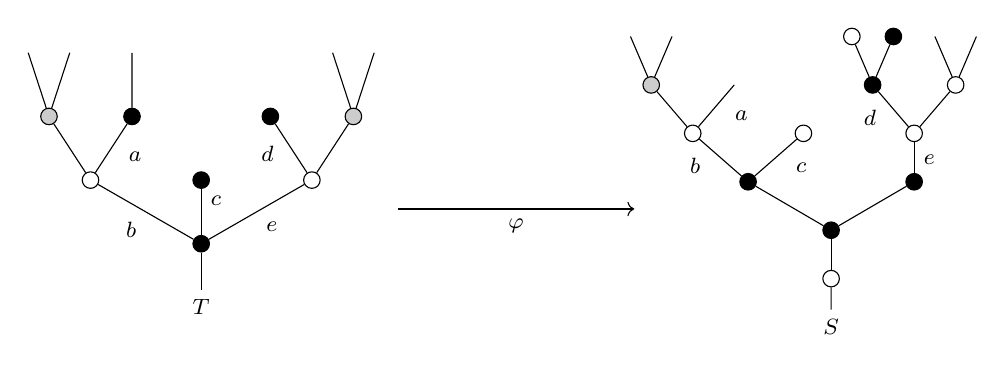
\begin{tikzpicture}[grow=up,auto,level distance=2.3em,
every node/.style = {font=\footnotesize},
dummy/.style={circle,draw,inner sep=0pt,minimum size=2.1mm}]
	\tikzstyle{level 2}=[sibling distance = 4em]
	\tikzstyle{level 3}=[sibling distance = 3em]
	\tikzstyle{level 4}=[sibling distance = 1.5em]
	\node at (0,0.25) {$T$}
		child{node [dummy,fill = black] {}
			child{node [dummy,fill=white] {}
				child{node [dummy,fill = black!20] {}
					child
					child
				}
				child{node [dummy,fill = black] {}
				edge from parent node [near end] {$d$}}
			edge from parent node [swap] {$e$}}
			child{node [dummy,fill=black] {}
			edge from parent node [swap, near end] {$c$}}
			child{node [dummy,fill=white] {}
				child{node [dummy,fill = black] {}
					child
				edge from parent node [swap, near end] {$a\phantom{d}$}}
				child{node [dummy,fill = black!20] {}
					child
					child
				}
			edge from parent node {$b$}}
		};
\begin{scope}[level distance=1.75em]
	\tikzstyle{level 3}=[sibling distance = 6em]
	\tikzstyle{level 4}=[sibling distance = 4em]
	\tikzstyle{level 5}=[sibling distance = 3em]
	\tikzstyle{level 6}=[sibling distance = 1.5em]
	\tikzstyle{level 7}=[sibling distance = 0.75em]
	\node at (8,0) {$S$}
		child{node [dummy,fill = white] {}
			child{node [dummy,fill = black] {}
				child{node [dummy,fill = black] {}
					child{node [dummy,fill=white] {}
						child{node [dummy,fill = white] {}
							child
							child
						}
						child{node [dummy,fill = black] {}
							child{node [dummy,fill=black] {}
						}
							child{node [dummy,fill=white] {}}
						edge from parent node [near end] {$d$}}
					edge from parent node [swap] {$e\phantom{1}$}}
				}
				child{node [dummy,fill = black] {}
					child{node [dummy,fill=white] {}
					edge from parent node [swap, near end] {$c\phantom{1}$}}
					child{node [dummy,fill=white] {}
						child{
						edge from parent node [swap,near end] {$a\phantom{d}$}}
						child{node [dummy,fill = black!20] {}
							child
							child
						}
					edge from parent node [near end] {$\phantom{1}b$}}
				}
			}
		};
\end{scope}
	\draw [->] (2.5,1.5) -- node [swap] {$\varphi$} (5.5,1.5);
\end{tikzpicture}
\]
\end{example}


\begin{remark}
By changing any $X$-labels in $S_{v_{G e}}$ 
into $Y$-labels (resp. $\mathcal{P}$-labels)
whenever $T_{v_{G}}$  has a 
$Y$-label (resp. $\mathcal{P}$-label), one obtains a factorization
\[ T \to \bar{S} \to S \]
such that $T \to \bar{S}$ is a label map 
(cf. Definition \ref{LABMAP DEF})
and $\bar{S} \to S$ is an underlying identity of trees that
merely changes some of the $Y$ and $\mathcal{P}$ labels into 
$X$-labels.
We refer to the latter kind of map as a \textit{relabel map}.
It is clear that the label-relabel factorization 
 is unique.
\end{remark}

\begin{proposition}
There is an identification
$\Omega_G^e \simeq 
|\Omega_{G}^{\mathsf{t},\lambda_l}|$.
\end{proposition}


\begin{proof}
We will show that Remark \ref{REALEX REM} applies to 
$\mathcal{C} = \Omega_G^e$,
with $\mathcal{C}_h$ and $\mathcal{C}^v$ the categories of 
relabel and label maps.
More precisely, we claim that there is an isomorphism 
$\mathcal{C}_{h,\bullet}^{v} \simeq 
\Omega_{G}^{\mathsf{t},\lambda_{\bullet}}$
of objects in $\mathsf{Cat}^{\Delta^{op}}$.
Unpacking notation, one must first show that strings
\begin{equation}\label{RELABSTR EQ}
T_0 \to T_1 \to \cdots \to T_l
\end{equation}
 of relabel arrows in $\Omega_G^e$
 are in bijection with objects of 
 $\Omega_{G}^{\mathsf{t},\lambda_l}$,
 i.e., with trees labeled by
 $\langle \langle l \rangle \rangle =
  \{-\infty, -l, \cdots, -1,0,1,\cdots,l,+ \infty\}$.
Noting that the maps in
(\ref{RELABSTR EQ})
are simply underlying identities on some fixed tree $T$
that convert some of the $\mathcal{P}$, $Y$ labels into $X$ labels,
we label a vertex $T_{v_{Ge}}$ by:
\begin{inparaenum}
\item[(i)]
$j$ such that
$0 < j \leq +\infty$
if the last $j$ labels of $T_{v_{Ge}}$ in 
(\ref{RELABSTR EQ}) are $Y$ labels (where $+\infty = l+1$); 
\item[(ii)]
$-j$ such that
$-\infty \leq -j < 0$
if the last $j$ labels of $T_{v_{Ge}}$ in 
(\ref{RELABSTR EQ}) are $\mathcal{P}$ labels;
\item[(iii)] $j=0$ if all labels in (\ref{RELABSTR EQ})
are $X$-labels.
\end{inparaenum}
 This process clearly establishes the desired bijection on objects.

The compatibilities with arrows and with the simplicial structure are straightforward.
\end{proof}

Letting 
$\tilde{N}^{(\mathcal P, X,Y)}$
be built from
$N_{\bullet,\bullet}^{(\mathcal P, X,Y)}$
via a double application of Proposition \ref{RANTRANS PROP}  thus yields the following, establishing 
(\ref{EXTTREEFOR EQ}).

\begin{corollary}
	$\mathcal P \coprod\limits_{\mathbb F X} \mathbb F Y \simeq \Lan_{(\Omega_G^e \to \Sigma_G)^{op}}\tilde N^{(\mathcal P, X,Y)}$.
\end{corollary}

Our next task is that of identifying a convenient initial subcategory $\widehat{\Omega}_G^{e} \hookrightarrow \Omega_G^e$.
We first introduce the auxiliary notion of alternating trees.
Recall the notion of input path (Notation \ref{INPUTPATH NOT})
$I(e) = \{f \in T \colon e \leq_d f\}$ for an edge $e \in T$, which naturally extends to $T$ in any of $\Omega, \Phi, \Omega_G, \Phi_G$.


\begin{definition}\label{OMEGAA DEF}
A $G$-tree $T \in \Omega_G$ is called \textit{alternating} if, for all leafs $l \in T$ one has that the input path $I(l)$ has an even number of elements.

Further, a vertex $e^{\uparrow} \leq e$ is called \textit{active}
if $|I(e)|$ is odd and \textit{inert} otherwise.

Finally, a tall map $T \xrightarrow{\varphi} S$ between alternating $G$-trees is called a 
\textit{tall alternating map}
if for any inert vertex $e^{\uparrow} \leq e$ of $T$ one has that 
$S_{e^{\uparrow} \leq e}$ is an inert vertex of $S$.

We will denote the category of alternating $G$-trees and tall alternating maps by $\Omega_G^a$.
\end{definition}

\begin{remark}
	A $G$-tree (resp. map) is alternating
	iff each component is.
\end{remark}

\begin{example}
Two alternating trees (for $G=\**$ the trivial group) and a planar tall alternating map between them follow, with active nodes in black ($\bullet$) and white nodes in white ($\circ$).
\[
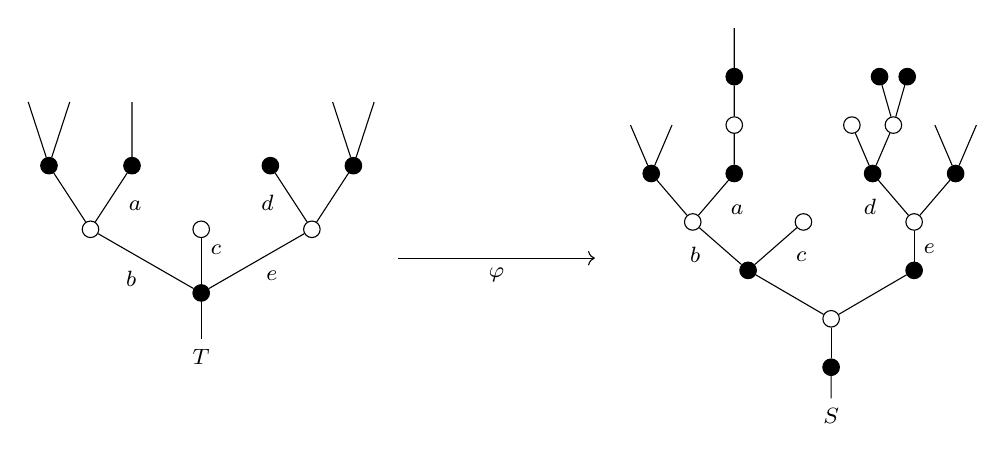
\begin{tikzpicture}[grow=up,auto,level distance=2.3em,every node/.style = {font=\footnotesize},dummy/.style={circle,draw,inner sep=0pt,minimum size=2.1mm}]
	\tikzstyle{level 2}=[sibling distance = 4em]
	\tikzstyle{level 3}=[sibling distance = 3em]
	\tikzstyle{level 4}=[sibling distance = 1.5em]
	\node at (0,0.75) {$T$}
		child{node [dummy,fill = black] {}
			child{node [dummy,fill=white] {}
				child{node [dummy,fill = black] {}
					child
					child
				}
				child{node [dummy,fill = black] {}
				edge from parent node [near end] {$d$}}
			edge from parent node [swap] {$e$}}
			child{node [dummy,fill=white] {}
			edge from parent node [swap, near end] {$c$}}
			child{node [dummy,fill=white] {}
				child{node [dummy,fill = black] {}
					child
				edge from parent node [swap, near end] {$a\phantom{d}$}}
				child{node [dummy,fill = black] {}
					child
					child
				}
			edge from parent node {$b$}}
		};
\begin{scope}[level distance=1.75em]
	\tikzstyle{level 3}=[sibling distance = 6em]
	\tikzstyle{level 4}=[sibling distance = 4em]
	\tikzstyle{level 5}=[sibling distance = 3em]
	\tikzstyle{level 6}=[sibling distance = 1.5em]
	\tikzstyle{level 7}=[sibling distance = 1em]
	\node at (8,0) {$S$}
		child{node [dummy,fill = black] {}
			child{node [dummy,fill = white] {}
				child{node [dummy,fill = black] {}
					child{node [dummy,fill=white] {}
						child{node [dummy,fill = black] {}
							child
							child
						}
						child{node [dummy,fill = black] {}
							child{node [dummy,fill=white] {}
								child{node [dummy,fill = black] {}}
								child{node [dummy,fill = black] {}}
						}
							child{node [dummy,fill=white] {}}
						edge from parent node [near end] {$d$}}
					edge from parent node [swap] {$e\phantom{1}$}}
				}
				child{node [dummy,fill = black] {}
					child{node [dummy,fill=white] {}
					edge from parent node [swap, near end] {$c\phantom{1}$}}
					child{node [dummy,fill=white] {}
						child{node [dummy,fill = black] {}
							child{node [dummy,fill=white] {}
								child{node [dummy,fill = black] {}
									child
								}
							}
						edge from parent node [swap,near end] {$a\phantom{d}$}}
						child{node [dummy,fill = black] {}
							child
							child
						}
					edge from parent node [near end] {$\phantom{1}b$}}
				}
			}
		};
\end{scope}
	\draw [->] (2.5,2) -- node [swap] {$\varphi$} (5,2);
\end{tikzpicture}
\]
The term ``alternating'' reflects the fact that adjacent nodes have different colors, though there is an additional restriction: the ``outer vertices'', i.e. those immediately below a leaf or above the root, are necessarily black/active
(this does not, however, apply to stumps).
%As for the map $\varphi$, we assume additionally that it is a planar map (so that by the tallness condition the root is sent to the root and leaves are sent to leaves while respecting the planar order) and that it sends the labeled edges of $T$ to the eponymous edges of $S$ (though this information is in fact redundant: only one such planar tall alternating map exists).
\end{example}


\begin{remark}\label{ALTSUB REM}
	If $T \in \Omega$ is alternating, it follows from 
	Remark \ref{INPPATH REM} that a tall map 
	$\varphi \colon T \to U$ is an alternating map
	iff the corresponding substitution datum 
	under Proposition \ref{SUBDATAUNDERPLAN PROP}
	is given by the identity 
	$U_{e^{\uparrow} \leq e } = T_{e^{\uparrow} \leq e}$
	when $e^{\uparrow} \leq e$ is inert 
	and by an alternating tree
	$U_{e^{\uparrow} \leq e }$ when 
	$e^{\uparrow} \leq e$ is active.
\end{remark}


\begin{definition}\label{HATOMEGAE DEF}
	$\widehat{\Omega}_G^e \hookrightarrow \Omega_G^e$ is the full subcategory of $(\mathcal{P},X,Y)$-labeled trees
	whose underlying tree is alternating, active nodes are labeled by $\mathcal{P}$,
	and inert nodes are labeled by $X$ or $Y$. 
\end{definition}

Note that conditions (i) and (ii) in Definition \ref{EXTTREECAT DEF} 
imply that for any map in $\widehat{\Omega}_G^e$
the underlying map is an alternating map.

The following is the key to establishing the desired initiality of 
$\widehat{\Omega}_G^e$ in $\Omega_G^e$.


\begin{proposition}\label{LXP PROP}
	For each $U \in \Omega_G^e$ there exists a unique 
	$\mathsf{lr}_{\mathcal{P}} (U) \in \widehat{\Omega}_G^e$ together with a unique planar label map in $\Omega_G^e$
\begin{equation}\label{LXP EQ}
	\mathsf{lr}_{\mathcal{P}} (U) \to U.
\end{equation}
	Furthermore, $\mathsf{lr}_{\mathcal{P}}$ extends to a right retraction 
	$\mathsf{lr}_{\mathcal{P}} \colon \Omega_G^e \to \widehat{\Omega}_G^e$.
\end{proposition}


Formally, the map \eqref{LXP EQ} in  Proposition \ref{LXP PROP}
will be built using Proposition \ref{BUILDABLE PROP}(iii),
which loosely says that planar tall maps $T \to U$
are determined by certain collections $\{U_i\}$
of outer faces of $U$,
with $T$ obtained by replacing 
$U_i$ with $\mathsf{lr}(U_i)$
(for the pictorial intuition, see Example \ref{GRAFTSUB EX}).
For the sake of intuition,
we first present an example.


\begin{example}\label{LRP EX}
	The following illustrates the $\mathsf{lr}_{\mathcal{P}}$ construction applied to the map $\varphi$ in
	Example \ref{REGALTERNMAP EX}. 
	Intuitively, 
	for each of the maximal $\mathcal{P}$-labeled outer subtrees
	$T^{\mathcal{P}}_k, S^{\mathcal{P}}_k$
	of $T,S$,
	the functor
	$\mathsf{lr}_{\mathcal{P}}$ replaces 
	$T^{\mathcal{P}}_k, S^{\mathcal{P}}_k$ with the corresponding leaf-root
	$\mathsf{lr}(T^{\mathcal{P}}_k),
	\mathsf{lr}(S^{\mathcal{P}}_k)$, which is again 
	$\mathcal{P}$-labeled.
	Pictorially, this results in the following two effects:
	when
	$T^{\mathcal{P}}_k, S^{\mathcal{P}}_k$ are single edge subtrees of $T,S$ (necessarily not adjacent to a $\mathcal{P}$-vertex)
	one degenerates that edge, adding a new $\mathcal{P}$-vertex of degree $1$;
	when
	$T^{\mathcal{P}}_k, S^{\mathcal{P}}_k$ have vertices,
	so that they are subtrees composed of adjacent 
	$\mathcal{P}$-vertices of $T,S$,
	those vertices are collapsed into a single  
	$\mathcal{P}$-vertex.
	\[
	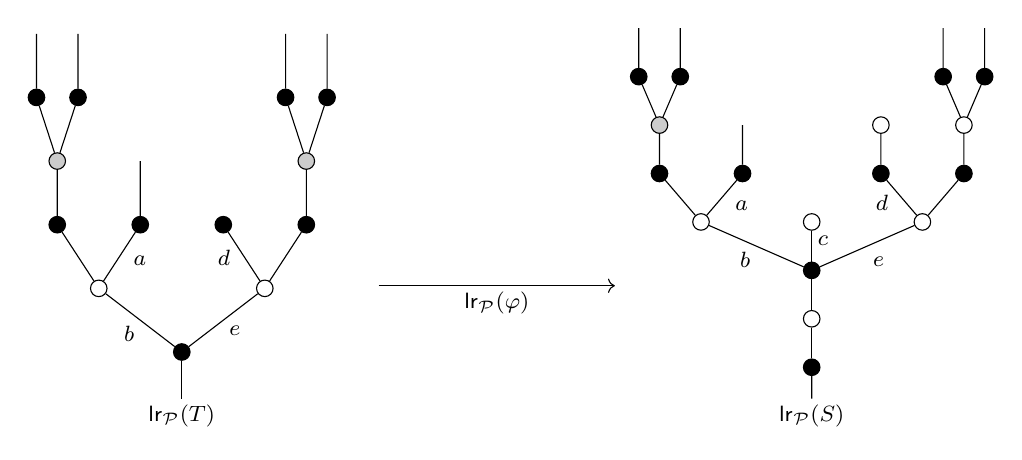
\begin{tikzpicture}[grow=up,auto,level distance=2.3em,
	every node/.style = {font=\footnotesize,inner sep=2pt},
	dummy/.style={circle,draw,inner sep=0pt,minimum size=2.1mm}]
	\tikzstyle{level 2}=[sibling distance = 6em]
	\tikzstyle{level 3}=[sibling distance = 3em]
	\tikzstyle{level 4}=[sibling distance = 1.5em]
	\node at (0,0.85) {$\mathsf{lr}_{\mathcal{P}}(T)$}
	child{node [dummy,fill = black] {}
		child{node [dummy,fill=white] {}
			child{node [dummy,fill = black] {}
				child{node [dummy,fill = black!20] {}
					child{node [dummy,fill = black] {}
						child}
					child{node [dummy,fill = black] {}
						child}
				}
			}
			child{node [dummy,fill = black] {}
				edge from parent node [near end] {$d$}}
			edge from parent node [swap] {$e$}}
		child{node [dummy,fill=white] {}
			child{node [dummy,fill = black] {}
				child
				edge from parent node [swap, near end] {$a\phantom{d}$}}
			child{node [dummy,fill = black] {}
				child{node [dummy,fill = black!20] {}
					child{node [dummy,fill = black] {}
						child}
					child{node [dummy,fill = black] {}
						child}
				}
			}
			edge from parent node {$b$}}
	};
	\begin{scope}[level distance=1.75em]
	\tikzstyle{level 3}=[sibling distance = 6em]
	\tikzstyle{level 4}=[sibling distance = 4em]
	\tikzstyle{level 5}=[sibling distance = 3em]
	\tikzstyle{level 6}=[sibling distance = 1.5em]
	\tikzstyle{level 7}=[sibling distance = 1.5em]
	\node at (8,0.85) {$\mathsf{lr}_{\mathcal{P}}(S)$}
	child{node [dummy,fill = black] {}
		child{node [dummy,fill = white] {}
			child{node [dummy,fill = black] {}
				child{node [dummy,fill=white] {}
					child{node [dummy,fill = black] {}
						child{node [dummy,fill = white] {}
							child{node [dummy,fill = black] {}
								child}
							child{node [dummy,fill = black] {}
								child}
						}
					}
					child{node [dummy,fill = black] {}
						child{node [dummy,fill=white] {}}
						edge from parent node [near end] {$d$}}
					edge from parent node [swap] {$e\phantom{1}$}}
				child{node [dummy,fill=white] {}
					edge from parent node [swap, near end] {$c\phantom{1}$}}
				child{node [dummy,fill=white] {}
					child{node [dummy,fill=black] {}
						child
						edge from parent node [swap,near end] {$a\phantom{d}$}}
					child{node [dummy,fill=black] {}
						child{node [dummy,fill = black!20] {}
							child{node [dummy,fill=black] {}
								child
							}
							child{node [dummy,fill=black] {}
								child
							}
						}
					}
					edge from parent node {$\phantom{1}b$}}
			}
		}
	};
	\end{scope}
	\draw [->] (2.5,2.5) -- node [swap] {$\mathsf{lr}_{\mathcal{P}}(\varphi)$} (5.5,2.5);
	\end{tikzpicture}
	\]
\end{example}




\begin{proof}[Proof of Proposition \ref{LXP PROP}]
	We first address the non-equivariant case $U \in \Omega^e$.

	To build $\mathsf{lr}_{\mathcal{P}}(U)$, consider the collection of outer faces
	$\{U_i^X\} \amalg \{U_j^Y\} \amalg \{U_k^{\mathcal{P}}\}$
where the $U_i^X$, $U_j^Y$ are simply the $X,Y$-labeled nodes,
and the $\{U_k^{\mathcal{P}}\}$ are the maximal outer subtrees whose nodes have only $\mathcal{P}$-labels (these may possibly be sticks). 
Lemma \ref{OUTERFACEUNION LEM} guarantees that 
each edge and each $\mathcal{P}$-labeled node belong to exactly
one of the $U_k^{\mathcal{P}}$, and applying 
Proposition \ref{BUILDABLE PROP}(iii)
yields a planar tall map
\begin{equation}\label{LRXDEF EQ}
T = \mathsf{lr}_{\mathcal{P}}(U) \to U
\end{equation}
such that $\{U_{e^{\uparrow} \leq e}\}_{(e^{\uparrow} \leq e) \in V(T)}
 = \{U_i^X\} \amalg \{U_j^Y\} \amalg 
 \{U_k^{\mathcal{P}}\}$. 
 $T$ has an obvious $(\mathcal{P},X,Y)$-labeling making 
(\ref{LRXDEF EQ}) into a label map, but we must still check $T \in \widehat{\Omega}^{e}_G$, i.e. that 
$T$ is alternating with active vertices precisely those labeled by $\mathcal{P}$.
But since the image of each $e \in T$
belongs to precisely one $U_k^{\mathcal{P}}$,
$e$ belongs to precisely one of the $\mathcal{P}$-labeled nodes of $T$, so that any leaf input path
$I(l) = (l = e_n \leq e_{n-1} \leq \cdots \leq e_1 \leq e_0)$
must start with, end with, and alternate between 
$\mathcal{P}$-nodes, and thus have even length.

To check uniqueness, note that for any other planar label map $S \to U$ with $S \in \widehat{\Omega}_G^e$
and $e^{\uparrow} \leq e$ a $\mathcal{P}$ vertex of $S$
the outer face 
$U_{e^{\uparrow} \leq e}$
must be a maximal 
$\mathcal{P}$-labeled outer face since the vertices adjacent to its root and leaves are labeled by either $X$ or $Y$.
The condition 
$V(U) = \coprod_{V(S)} V(U_{e^{\uparrow} \leq e})$
thus guarantees that the collection of outer faces determined by $S$ matches that determined by $T$
except perhaps in the number of stick faces, so that 
the degeneracy-face factorizations
$S \to F \to U$, $T \to F \to U$
factor through the same planar inner face $F$, with the  unique labeling that makes the inclusion a label map.
$S$, $T$ are thus both trees in $\widehat{\Omega}_G^e$ obtained from $F$ by adding degenerate $\mathcal{P}$ vertices, 
and since this can be done in at most one way, we conclude 
$S=T$. 

To check functoriality,
consider the diagram below, where $T \to U$ is the map defined above and $\varphi \colon U \to V$ any map in $\Omega_G^e$.
\begin{equation}\label{LRPFUN EQ}
\begin{tikzcd}
	T \ar{r} \ar[dashed]{d} &  U \ar{d}{\varphi}
\\
	S \ar[dashed]{r} & V
\end{tikzcd}
\end{equation}
The composite $T \to V$ is encoded by a substitution datum
$\{T_{e^{\uparrow} \leq e} \to V_{e^{\uparrow} \leq e}\}$
which is given by an isomorphism
if $e^{\uparrow} \leq e$ has label $X$ or $Y$ (possibly changing a $Y$ label to a $X$ label),
and by some $(X,\mathcal{P})$-labeled tree 
$V_{e^{\uparrow} \leq e}$ if $e^{\uparrow} \leq e$
has a $\mathcal{P}$-label.
We now consider the factorization problem 
in (\ref{LRPFUN EQ}), where we want $S \in \widehat{\Omega}_G^e$
and for the map $S \to V$ to the a planar label map.
Combining Remark \ref{ALTSUB REM} with the uniqueness of the
$\mathsf{lr}_{\mathcal{P}}(V_{e^{\uparrow} \leq e})$,
the only possibility is for $S$ to be defined using the 
$T$ substitution datum
that replaces 
$T_{e^{\uparrow} \leq e} \to V_{e^{\uparrow} \leq e}$
with 
$T_{e^{\uparrow} \leq e} \to 
\mathsf{lr}_{\mathcal{P}}(V_{e^{\uparrow} \leq e})$
whenever $e^{\uparrow} \leq e$ has a $\mathcal{P}$-label.
Uniqueness of $\mathsf{lr}_{\mathcal{P}} (V)$ then implies 
$S=\mathsf{lr}_{\mathcal{P}} (V)$, and one sets 
$\mathsf{lr}_{\mathcal{P}} (\varphi)$
to be the map $T\to S$.
Associativity and unitality are automatic from the uniqueness of the factorization of (\ref{LRPFUN EQ}).

For $T = (T_x)_{x \in X}$ in 
$\Omega_G^e$ with $G$ a general group,
one sets
$\mathsf{lr}_{\mathcal{P}}(T) = (\mathsf{lr}_{\mathcal{P}}(T_x))_{x \in X}$.
\end{proof}



\begin{corollary}\label{KANRED COR}
The inclusion 
$\widehat{\Omega}_G^e \hookrightarrow \Omega_G^e$ 
is $\mathsf{Ran}$-initial over $\Sigma_G$.
In other words, for $\C$ any complete category and 
functor $N \colon \Omega_G^e \to \C$ it is
\[
\mathsf{Ran}_{\Omega_G^e \to \Sigma_G} N
	\simeq 
\mathsf{Ran}_{\widehat{\Omega}_G^e \to \Sigma_G} N.
\]
\end{corollary}

\begin{proof}
	Since $\mathsf{lr}_{\mathcal{P}}$ is a right retraction over $\Sigma_G$, the undercategories 
	$C \downarrow \widehat{\Omega}_G^e$ are right retractions of 
	$C \downarrow \Omega_G^e$ for any $C \in \Sigma_G$.
\end{proof}

\renewcommand{\labelenumi}{\theenumi}
\renewcommand{\theenumi}{(\roman{enumi})}%

\subsection{Filtrations of free extensions}
\label{FILTRATION_SECTION}

Summarizing \S \ref{EXTTREE SEC},
%the previous section, 
the discussion after Proposition \ref{RANTRANS PROP}
establishes (\ref{EXTTREEFOR EQ}), and hence 
Corollary \ref{KANRED COR} 
gives the alternative formula
(the use of opposite categories turns 
$\mathsf{Ran}$ into $\mathsf{Lan}$)
\begin{equation}\label{ALTFOR EQ}
	\mathcal{P}[u] \simeq
	\mathcal{P} \mathbin{\check{\coprod}}_{\mathbb{F}_G X} \mathbb{F}_G Y 
\simeq 
	\mathsf{Lan}_{\left( \widehat{\Omega}_{G}^{e} \to \Sigma_G \right)^{op}}
	\tilde{N}^{(\mathcal{P},X,Y)},
\end{equation}
which we will now use to 
filter the map
$\mathcal{P} \to \mathcal{P}[u]$
in the underlying category
$\Sym_G(\V)$.

First, given 
$T = (T_i)_{i \in I} \in \Omega_G^e$,
we write $V^X(T_i)$ (resp. $V^Y(T_i)$)
to denote the set of 
$X$-labeled ($Y$-labeled) vertices of $T_i$.
We define \textit{degrees} of $T$ by
\[
|T|_X = |V^X(T_i)|,
	\qquad
|T|_Y = |V^Y(T_i)|,
	\qquad
|T| = |T|_X + |T|_Y,
\]
which we note do not depend on the choice of $i \in I$.

Similarly, for $T = (T_i)_{i \in I} \in \Omega_G^a$
we write $V^{in}(T_i)$ for the inert vertices and
$|T| = |V^{in}(T_i)|$.

\begin{remark}
	One key property of the degrees $|T|$, $|T|_X$, $|T|_Y$ is that they are invariant under root pullbacks, which are defined
	by generalizing Definition \ref{ROOTPULL DEF}
	in the obvious way.
\end{remark}


\begin{definition}\label{TREE_FILTRATION_PIECES_DEFINITION}
We specify some rooted (i.e. closed under root pullbacks)
full subcategories
 of $\widehat{\Omega}_{G}^e$: 
  \begin{enumerate}
  \item $\widehat{\Omega}_G^e[\leq\! k]$ 
  (resp. $\widehat{\Omega}_G^e[k]$) is the subcategory of $T$ with $|T|\leq k$ ($|T| = k$);
  \item $\widehat{\Omega}_G^e[\leq\! k \mathbin{\backslash} Y]$
  (resp. $\widehat{\Omega}_G^e[k \mathbin{\backslash} Y]$) is the subcategory of $\widehat{\Omega}_G^e[\leq\! k]$ 
  ($\widehat{\Omega}_G^e[k]$) of $T$ with $|T|_{Y}\neq k$.
%  \item $\widehat{\Omega}_G^e[k,0]$ is the  subcategory of 
%  $\widehat{\Omega}_G^e[k]$ of $T$ with $|T|_X = 0$ (or, equivalently, $|T|_{Y} = k$).
%  \item If $\Xi$ is any of the above categories, and $C\in \Sigma_G$, let $\Xi(C)$ denote the full subcategory of $\Xi$ spanned by those trees $T$ with $val(T) \simeq C$.
  \end{enumerate}
Similarly, we define subcategories 
$\Omega_G^a[\leq \! k]$, 
$\Omega_G^a[k]$ of $\Omega_G^a$
by the conditions $|T|\leq k$, $|T|=k$.
\end{definition}


\begin{remark}\label{LIMMOR REM}
  The categories 
  $\widehat{\Omega}_G^e[k]$, $\widehat{\Omega}_G^e[k \mathbin{\backslash} Y]$ and $\Omega_G^a[k]$
  have rather limited morphisms.
  
Indeed, it is clear from Definitions 
\ref{EXTTREECAT DEF} and \ref{OMEGAA DEF} 
that maps never lower degree,
and Remark \ref{ALTSUB REM} further ensures that degree is preserved iff
$\mathcal{P}$-vertices are substituted by $\mathcal{P}$-vertices (rather than larger trees
which would necessarily have inert vertices, thus increasing degree).
Therefore, all maps in $\Omega_G^a[k]$ are quotients while maps in $\widehat{\Omega}_G^e[k]$, $\widehat{\Omega}_G^e[k \mathbin{\backslash} Y]$
are underlying quotients of $G$-trees that 
relabel some $Y$-vertices to $X$-vertices.  
 Moreover, this can be repackaged as saying that 
  the diagonal forgetful functors in
\[
\begin{tikzcd}
  \widehat\Omega_G^e[k \mathbin{\backslash} Y] \arrow[dr] \arrow[rr, hookrightarrow] 
  && \widehat\Omega_G^e[k] \arrow[dl]\\
  & \Omega_G^a[k]
\end{tikzcd}
\]  
 are Grothendieck fibrations whose fibers over 
 $T \in \Omega_G^a[k]$
 are the punctured cube and cube categories
\[
	(Y \to X)^{\times V_G^{in}(T)} - Y^{\times  V_G^{in}(T)},
\qquad
	(Y \to X)^{\times V_G^{in}(T)}
\]
for $V_G^{in}(T)$ the set of inert $G$-vertices.

Note that though 
$|V^{in}(T_i)| = k$
for each of the $T_i$ that constitute $T=(T_i)_{i \in I}$,
one can only guarantee $|V_G^{in}(T)| \leq k$.
\end{remark}


\begin{lemma}\label{MINUS_LAN_FINAL_LEMMA}
%  $\widehat{\Omega}_G^e[\leq\! k-1]$ is $\mathsf{Ran}$-initial in $\widehat{\Omega}_G^{e}[\leq\! k \mathbin{\backslash} Y]$ over $\Sigma_G$ (cf. Corollary \ref{KANRED COR}).
% 
The horizontal inclusion below 
\[
\begin{tikzcd}
	\widehat{\Omega}_G^e[\leq\! k-1]
	\arrow{dr}[swap]{\mathsf{lr}} \arrow[rr, hookrightarrow] &&
	\widehat{\Omega}_G^{e}[\leq\! k \mathbin{\backslash} Y] \arrow{dl}{\mathsf{lr}}
\\
	&
	\Sigma_G
\end{tikzcd}
\]  
is $\mathsf{Ran}$-initial (in the sense of Corollary \ref{KANRED COR})
over $\Sigma_G$.  
\end{lemma}

The proof will make use of an additional construction on 
$\Omega_{G}^e$: given $T \in \Omega_{G}^e$ let $T_{\mathcal{P}}$ denote the result of replacing all $X$-labeled nodes of $T$ with $\mathcal{P}$-labeled nodes.

\begin{remark}\label{YINERT REM}
	In contrast to the functor
	$\mathsf{lr}_{\mathcal{P}} \colon
	\Omega_G^e \to \widehat{\Omega}_G^e $
	of Proposition \ref{LXP PROP},
	the $(\minus)_{\mathcal{P}}$ construction 
	does not define a full functor
        $\Omega_G^e \to \Omega_G^e$, instead only being functorial, and the obvious maps $T_{\mathcal{P}} \to T$ only being natural,
        with respect to the
        maps of $\Omega_G^e$ that preserve $Y$-labels.
\end{remark}


\begin{example}
Combining the $(\minus)_{\mathcal{P}}$ and $\mathsf{lr}_{\mathcal{P}}$ constructions one obtains a construction sending trees in $\widehat{\Omega}^e_G$ to trees in $\widehat{\Omega}^e_G$.
We illustrate this for the tree $T \in \widehat{\Omega}^e$ below (so that $G=\**$), where black nodes are $\P$-labeled, white nodes are $X$-labeled, and grey nodes are $Y$-labeled.
\[
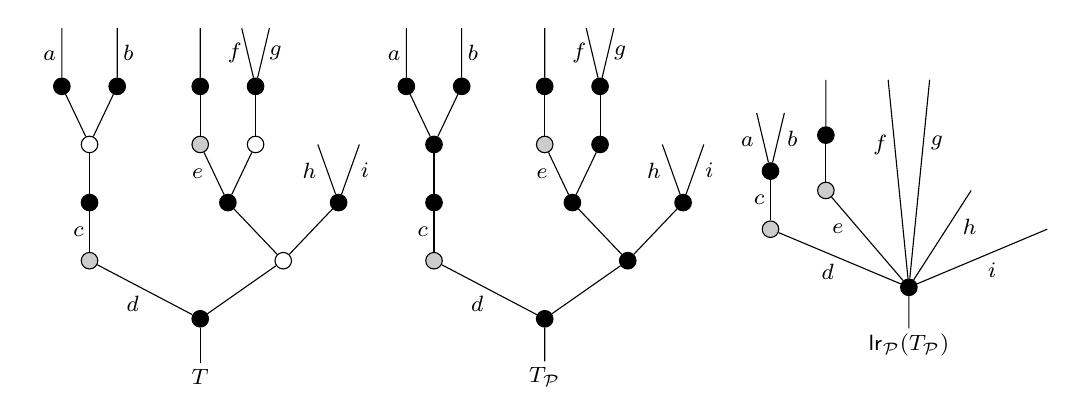
\begin{tikzpicture}
  [grow=up,auto,level distance=2.1em,
  every node/.style = {font=\footnotesize,inner sep=2pt},
  dummy/.style={circle,draw,inner sep=0pt,minimum size=2.1mm}]
  % [grow=up, level distance = .8cm, auto, every node/.style={font=\small}, dummy/.style={circle,draw,inner sep=0.4mm, minimum size=2.25}]
  \tikzstyle{level 2}=[sibling distance=6em]
  \tikzstyle{level 3}=[sibling distance=4em]
  \tikzstyle{level 4}=[sibling distance=2em]
  \tikzstyle{level 5}=[sibling distance=2em]
  \tikzstyle{level 6}=[sibling distance=1em]
  \node at (0,0){$T$}
  child{node [dummy, fill=black] {}%
    child{node [dummy, fill=white] {}%
      child{node [dummy,fill=black] {}%
        child[sibling distance = 1.5em]{edge from parent node [swap,near end] {$i$}}
        child[sibling distance = 1.5em]{edge from parent node [near end] {$h$}}
      }
      child{node [dummy, fill=black] {}%
        child{node [dummy, fill=white] {}%
          child{node [dummy, fill=black] {}%
            child{edge from parent node [right]{$g$}} 
            child{edge from parent node [left]{$f$}} 
          }
        }
        child{node [dummy, fill=black!20] {}%
          child{node [dummy, fill=black] {}%
            child{}
          }
          edge from parent node [near end] {$e$}
        }
      }
    }
    child[sibling distance=8em]{node [dummy, fill=black!20] {}%
      child{node [dummy, fill=black] {}%
        child{node [dummy, fill=white] {}%
          child{node [dummy, fill=black] {}%
            child{edge from parent node [swap] {$b$}}
          }
          child{node [dummy, fill=black] {}%
            child{edge from parent node {$\phantom{b}a$}}
          }
        }
        edge from parent node {$c$}
      }
      edge from parent node {$d$}
    }
  };
  \node at (4.375,0){$T_{\mathcal{P}}$}
  child{node [dummy, fill=black] {}%
    child{node [dummy, fill=black] {}%
      child{node [dummy,fill=black] {}%
        child[sibling distance = 1.5em]{edge from parent node [swap,near end] {$i$}}
        child[sibling distance = 1.5em]{edge from parent node [near end] {$h$}}
      }
      child{node [dummy, fill=black] {}%
        child{node [dummy, fill=black] {}%
          child{node [dummy, fill=black] {}%
            child{edge from parent node [right]{$g$}} 
            child{edge from parent node [left]{$f$}} 
          }
        }
        child{node [dummy, fill=black!20] {}%
          child{node [dummy, fill=black] {}%
            child{}
          }
          edge from parent node [near end] {$e$}
        }
      }
    }
    child[sibling distance=8em]{node [dummy, fill=black!20] {}%
      child{node [dummy, fill=black] {}%
        child{node [dummy, fill=black] {}%
          child{node [dummy, fill=black] {}%
            child{edge from parent node [swap] {$b$}}
          }
          child{node [dummy, fill=black] {}%
            child{edge from parent node {$\phantom{b}a$}}
          }
        }
        edge from parent node {$c$}
      }
      edge from parent node {$d$}
    }
  };
  \tikzstyle{level 2}=[sibling distance=2em]
  \tikzstyle{level 4}=[sibling distance=1em]
	\node at (9,0.4){$\mathsf{lr}_{\mathcal{P}}(T_{\mathcal{P}})$}
	child{node [dummy,fill=black] {}%
		child{edge from parent node [swap]{$i$}}
		child[sibling distance =1.5em, level distance =3.5em]{edge from parent node [near end,swap] {$h$}}
	    child[sibling distance=1.5em, level distance = 7.5em]{edge from parent node [swap, near end]{$g$}}
		child[sibling distance=1.5em, level distance = 7.5em]{edge from parent node [near end]{$f$}}
    child[level distance = 3.5em]{node [dummy, fill=black!20] {}%
      child[level distance = 2em]{node [dummy, fill=black] {}%
        child{}
      }
      edge from parent node [near end]{$e$}
    }
    child{node [dummy, fill=black!20] {}%
      child{node [dummy, fill=black] {}%
        child{edge from parent node [swap,near end]{$b$}}
        child{edge from parent node [near end] {$\phantom{b}a$}}
        edge from parent node {$c$}
      }
      edge from parent node {$d$}
    }
  };    
\end{tikzpicture}
\]
\end{example} 

\begin{proof}[Proof of Lemma \ref{MINUS_LAN_FINAL_LEMMA}]

By Proposition \ref{FIBERKANMAP PROP} it suffices to
show that for each $C \in \Sigma_G$
the map of rooted undercategories
\[
C \downarrow_{\mathsf{r}} \widehat{\Omega}_G^e[\leq\! k-1]
	\to 
C \downarrow_{\mathsf{r}} \widehat{\Omega}_G^e[\leq\! k \mathbin{\backslash} Y]
\]
is initial, i.e. 
(cf. \cite[IX.3]{McL}) that for each
$(S,\pi \colon C \to \mathsf{lr}(S))$ in 
$C \downarrow_{\mathsf{r}} \widehat{\Omega}_G^e[\leq\! k \mathbin{\backslash} Y]$
the overcategory
\begin{equation}\label{UNDERCATPR EQ}
	(C \downarrow_{\mathsf{r}} \widehat{\Omega}_G^e[\leq\! k-1])
		\downarrow
	(S,\pi)  
\end{equation}
is non-empty and connected. 
By definition of rooted undercategory, $\pi$ is the identity on roots and thus an isomorphism on $\Sigma_G$,
so that objects of (\ref{UNDERCATPR EQ})
correspond to maps
$T \to S$
that induce a rooted isomorphism on 
$\mathsf{lr}$, i.e. rooted tall maps.

The case $S\in \widehat{\Omega}_G^e[\leq\! k-1]$ is immediate,
since then the identity $S = S$ is terminal in 
(\ref{UNDERCATPR EQ}).
Otherwise, since $|S|_Y \neq k$ we have
$|\mathsf{lr}_{\mathcal{P}}(S_{\mathcal{P}})|<k$
and the map 
$\mathsf{lr}_{\mathcal{P}}(S_{\mathcal{P}}) \to S$,
which is a rooted tall, shows that
(\ref{UNDERCATPR EQ}) is indeed non-empty.

 
Now, consider a rooted tall map $T \to S$ with 
$T \in \widehat{\Omega}_G^e[\leq\! k-1]$. One can form a diagram
\begin{equation}\label{K-1LANFINAL EQ}
\begin{tikzcd}
      & S & \mathsf{lr}_{\mathcal{P}}(S_{\mathcal{P}}) \ar{l}
      \\
      T \ar{ur} \ar{r} & T' \ar{u}[swap]{Y-\text{pres}} & \mathsf{lr}_{\mathcal{P}}(T'_{\mathcal{P}}) \ar{l} \ar{u}
\end{tikzcd}
\end{equation}
where $T \to T' \to S$ is the natural factorization such that $ T' \to S$ preserves $Y$-labels, 
i.e., $T'$ is obtained from $T$ by simply relabeling to $X$ those $Y$-labeled vertices of $T$ that become $X$-vertices in $S$.
Note that by Remark \ref{YINERT REM}, the existence
of the right square relies on 
$T' \to S$ preserving $Y$-labels.
Since all maps in 
(\ref{K-1LANFINAL EQ})
are rooted tall, 
this produces the
necessary zigzag connecting the objects $T \to S$ and 
$\mathsf{lr}_{\mathcal{P}}(S_{\mathcal{P}}) \to S$
in the category (\ref{UNDERCATPR EQ}), finishing the proof.
%
%
%Further, given any other element
%\begin{equation}
%    \label{K-1_LAN_FINAL_EQ2}
%    \begin{tikzcd}
%      val(S) && val(T) \arrow[ll, "f"']\\
%      & C \arrow{ur}[swap]{q_S} \arrow[ul, "q_T"]
%    \end{tikzcd}
%  \end{equation}
%  in the overcategory, consider the following zig-zag of maps connecting the objects (\ref{K-1_LAN_FINAL_EQ1}) and (\ref{K-1_LAN_FINAL_EQ2}):
%\begin{equation}\label{K-1_LAN_FINAL_DIAGRAM}
%\begin{tikzcd}
%	&& S &&
%\\[20pt]
%	&& \tilde q_T^*(S) \arrow[u, "\tilde q_T"'] &&
%\\
%	S^\wedge_\P \arrow[uurr, "\partial_\P"] &
%	\tilde q_T^*(S^\wedge_\P) \arrow[l, "\tilde q_T"'] \arrow[ur, "\partial_\P"] \arrow[rr, "\partial_\P"] &&
%	 T' \arrow[ul, "\partial_\P"'] & T \arrow[l, "\partial_Y"'] \arrow[uull, "f"']
%\\[20pt]
%	&& C \arrow[ull, "q_S"] \arrow[ul, "q_T"'] \arrow[ur, "q_T"] \arrow[urr, "q_T"'] 
%\end{tikzcd}
%\end{equation}
%  Here, we have omitted the notation ``$val$'' from the top three rows. To understand this diagram, we first record that we have a factorization:
%  \[
%  q_S = \tilde q_T q_T,
%  \]
%  Then, if we let $C_S = val(S) = val(S^\wedge_\P)$ and $C_T = val(T)$, we have
%  \[
%  C \xrightarrow{q_T} C_T \xrightarrow{\tilde q_T} C_S
%  \]
%  and hence, by the unique factorization of maps in $\Omega_{G,e}$, a factorization% via Remark \ref{OMEGA_E_REMARKS} (2), a factorization
%  \[
%  \begin{tikzcd}
%    C_T \arrow[d, "\tilde q_T"'] \arrow[r, dashed] & \tilde q_T^*(S^\wedge_\P) \arrow[d, dashed, "\tilde q_T"]\\
%    C_S \arrow[r] & S^\wedge_\P
%  \end{tikzcd}
%  \]
%  (where we are recording $C \to val(S)$ as a planar-tall map $C \to S$). 
%  A similar analysis shows that the top left trapezoid commutes. 
%
%  The other regions also commute by a straightforward analysis. Indeed, the top right trapezoid commutes by unique factorization, and finally the middle triangle of $\partial_\P$ maps commutes since $(\tilde q_T^*S)^\wedge_\P = \tilde q^*_T(S^\wedge_\P)$. 
%  
%  Lastly, we must check that the middle two maps are in fact elements of the appropriate overcategory. This follows from the fact that $S^\wedge_\P$ and $T$ have $|-|_Y < k$. Thus, the overcategory in question is connected, as desired.
\end{proof}

%Similarly to the $(\minus)_{\mathcal{P}}$ construction,
%there is also a construction $T_Y$ which replaces all $X$-labels of $T \in \Omega_G^e$ with $Y$-labels. Moreover, in this case the construction restricts directly to a construction on 
%$\bar{\Omega}_G^e$,
%which is easily seen to be functorial (and the $T_Y \to T$ maps natural) with regards to $\mathcal{P}$-inert maps. Remark \ref{LIMMOR REM} thus implies that 
%$(\minus)_Y \colon \bar{\Omega}_G^e[k] \to 
%\bar{\Omega}_G^e[k,0]$
%is a left retraction, 
%resulting in the following.
%\begin{lemma}
%  \label{ZERO_LAN_FINALITY_LEMMA}
%  $\bar{\Omega}_G^{e}[k,0]$ is $\mathsf{Ran}$-initial in $\bar{\Omega}_G^e[k]$ over $\Sigma_G$. 
%\end{lemma}

%\begin{proof}[Proof of Lemma \ref{ZERO_LAN_FINALITY_LEMMA}]
%  This follows analogously to Lemma \ref{MINUS_LAN_FINAL_LEMMA}, by replacing Diagram \ref{K-1_LAN_FINAL_DIAGRAM} with the diagram below:
%  \[
%  \begin{tikzcd}
%    && S & \\[20pt]
%    &&\tilde q_T^*(S) \arrow[u, "\tilde q_T"]\\
%    S^\wedge_Y \arrow[uurr, "\partial_Y"] && \tilde q_T^*(S^\wedge_Y) \arrow[ll, "\tilde q_T"'] \arrow[u, "\partial_Y"] \arrow[rr, "\partial_Y"] && T \arrow[ull, "\partial_Y"'] \arrow[uull, "f"']\\
%    && C \arrow[ull, "q_S"] \arrow[u, "q_T"] \arrow[urr, "q_T"'] 
%  \end{tikzcd}
%  \]
%\end{proof}

In what follows we write $\tilde{N} \colon \widehat{\Omega}_G^{e,op} \to \mathcal{V}$ for the functor in (\ref{ALTFOR EQ}) and any of its restrictions.

We are now in a position to produce the filtration (\ref{FILTR EQ})
of the map $\mathcal{P} \to \mathcal{P}[u]$
in (\ref{FREE_FG_EXT_EQ}).

\begin{definition} \label{PK_DEFN}
  Let $\P_k$ denote the left Kan extension
\[
\begin{tikzcd}[column sep =4em]
	|[alias=U]| \widehat{\Omega}_G^e[\leq\! k]^{op} \arrow[r, "\tilde{N}"] \arrow[d, "\mathsf{lr}"'] & \V
\\
	\Sigma_G^{op} \arrow[ur, "\P_k"', ""{name=V}]
	\arrow[Rightarrow, from=U, to=V]
\end{tikzcd}
\]
\end{definition}
Noting that $\widehat{\Omega}_G^e[\leq\! 0] \simeq \Sigma_G$
(since $|T|=0$ only if $T$ is a $G$-corolla with $\mathcal{P}$-labeled vertex)
and that $\widehat{\Omega}_G^e$
is the union of (the nerves of) the 
$\widehat{\Omega}_G^e[\leq\! k]$,
we obtain the desired filtration
\begin{equation}\label{FILT EQ}
	\mathcal{P} = 
	\mathcal{P}_0 \to 
	\mathcal{P}_1 \to
	\mathcal{P}_2 \to
	\cdots \to 
	\colim_k \mathcal{P}_k = \mathcal{P}[u].
\end{equation}

To analyze (\ref{FILT EQ}) homotopically we will further need a pushout description of each map 
$\mathcal{P}_{k-1} \to \mathcal{P}_k$. To do so,  note that the diagram of inclusions
\begin{equation}\label{INCDIAG EQ}
\begin{tikzcd}
	\widehat{\Omega}_G^{e}[k \mathbin{\backslash} Y]
	\arrow[d] \arrow[r] &
	\widehat{\Omega}_G^{e}[\leq\! k \mathbin{\backslash} Y]
	\arrow[d]
\\
	\widehat{\Omega}_G^e[k] \arrow[r] &
	\widehat{\Omega}_G^e[\leq\! k]
\end{tikzcd}
\end{equation}
is a pushout of at the level of nerves.
Indeed, this follows since
\[
	\widehat{\Omega}_G^e[k] \cap
	\widehat{\Omega}_G^{e}[\leq\! k \mathbin{\backslash} Y]
	= \widehat{\Omega}_G^{e}[k \mathbin{\backslash} Y],
\qquad
	\widehat{\Omega}_G^e[k] \cup 
	\widehat{\Omega}_G^{e}[\leq\! k\mathbin{\backslash} Y]
	= \widehat{\Omega}_G^{e}[\leq\! k],
\]
and since a map $T \to S$ in 
$\widehat{\Omega}_G^e[\leq\! k]$ is in one of subcategories in (\ref{INCDIAG EQ}) if and only if $T$ is.

Since Lemma \ref{MINUS_LAN_FINAL_LEMMA} provides an identification 
$\mathsf{Lan}_{\widehat{\Omega}_{G}^{e}[\leq\! k \mathbin{\backslash} Y]^{op}}\tilde{N} \simeq
\mathsf{Lan}_{\widehat{\Omega}_{G}^{e}[\leq\! k-1]^{op}}\tilde{N} = \mathcal{P}_{k-1}$,
applying left Kan extensions to (\ref{INCDIAG EQ}) yields the pushout diagram below.
\begin{equation}\label{FILTRATION_LAN_SQUARE_DIAGRAM}
\begin{tikzcd}
	\mathsf{Lan}_{\widehat{\Omega}_{G}^e[k \mathbin{\backslash} Y]^{op}}\tilde{N} \arrow[d] \arrow[r] & 
	\P_{k-1} \arrow[d]
\\
	\mathsf{Lan}_{\widehat{\Omega}_{G}^e[k]^{op}}\tilde{N} \arrow[r] &
	\P_k
\end{tikzcd}
\end{equation}

We will also make use of an 
explicit levelwise description of  
(\ref{FILTRATION_LAN_SQUARE_DIAGRAM}).

%Finally, we show that each layer $\Omega_G^e[\leq k]$ can be built from $\Omega_{G}^e[\leq k-1]$ via a pushout which attaches trees with precise degree $k$. 
%While dealing with general pushouts of categories requires solving a ``word problem'' on morphisms, we will only work in cases where the problem collapses. We recall that, given a square of categories
%\[
%\begin{tikzcd}
%  \mathcal A \arrow[d] \arrow[r] & \mathcal C \arrow[d]\\
%  \mathcal C \arrow[r] & \mathcal D
%\end{tikzcd}
%\]
%if the nerve of this square is a pushout in $\sSet$, then this is a pushout of categories (since the nerve is the inclusion of a reflective subcategory).

%If we further assume that the span of functors is built out of fully-faithful inclusions, these pushouts behave as nicely as possible with left Kan extensions.
%\begin{lemma}
%  \label{LAN_PUSHOUT_LEMMA}
%  Given any diagram in categories of the form 
%\[
%\begin{tikzcd}
%  \mathcal A \arrow[d] \arrow[r, "f"] & \mathcal C \arrow[d, %"i"]\\
%  \mathcal B \arrow[r, "g"] & \mathcal D \arrow[r, "Y"] \arrow[d, "j"] & \V \\
%  & \mathcal D
%\end{tikzcd}
%\]
%such that the square is a nerve pushout of fully-faithful %functors, then $\Lan_j Y$ is the pushout of the induced span
%\[
%\begin{tikzcd}
%  \Lan_{j i f}(Y i f) \arrow[r] \arrow[d] & \Lan_{j i}(Y i)\\
%  \Lan_{j g}(Y g).
%\end{tikzcd}
%\]
%\end{lemma}
%\begin{proof}
%  By the universal property of left Kan extensions, it suffices to show that, for any functor $Z: \V \to \D$, the natural map
%  \[
%  \V^\D(Y, Z j) \longto \V^{\mathcal B} (Y g, Z j g) \prod\limits_{\V^{\mathcal A}(Y i f, Z j i f)} \V^{\mathcal C}(Y i, Z j i)
%  \]
%  is a bijection. These two sets give the same data: a collection of maps $\Phi_b: Y(b) \to Z(b)$ and $\Phi_c:Y(c) \to Z(c)$ for all $b\in \mathcal B$ and $c \in \mathcal C$, such that $\Phi_b = \Phi_c$ whenever $b = c \in \mathcal A$. In general, the compatibilites required on the right are less demanding. However, with the above assumptions, a map $d \to d'$ in $\mathcal D$ is \textit{uniquely} a map in $\mathcal A$, $\mathcal B \setminus \mathcal A$, or $\mathcal C \setminus \mathcal A$, and thus all the necessary compatibilities are covered by (at least) one of the $\set{\Phi_b}$ or $\set{\Phi_c}$. 
%\end{proof}


\begin{proposition}
For each $G$-corolla $C \in \Sigma_G$,
(\ref{FILTRATION_LAN_SQUARE_DIAGRAM})
is given by the following pushout in $\V^{\mathsf{Aut}(C)}$
\begin{equation}\label{FILTRATION_LAN_LEVEL}
\begin{tikzcd}
	\coprod\limits_{[T] \in \mathsf{Iso}
		\left(C \downarrow_{\mathsf{r}} \Omega_G^a[k]\right)}
	\left(
		\bigotimes\limits_{v \in V_{G}^{ac}(T)}\P(T_v) \otimes
		Q_T^{in}[u]
	\right)
		\mathop{\otimes}\limits_{\mathsf{Aut}(T)} \mathsf{Aut}(C)
	\arrow[r] \arrow[d] &
	\P_{k-1}(C) \arrow[d] 
\\
	\coprod\limits_{[T] \in \mathsf{Iso}
		\left(C \downarrow_{\mathsf{r}} \Omega_G^a[k]\right)}
	\left(
		\bigotimes\limits_{v \in V_{G}^{ac}(T)}\P(T_v) \otimes
		\bigotimes\limits_{v \in V_{G}^{in}(T)} Y(T_v)
	\right)
		\underset{\mathsf{Aut}(T)}{\otimes} \mathsf{Aut}(C)
	\arrow[r] &
	\P_k(C)
\end{tikzcd}
\end{equation}
where $ V_{G}^{ac}(T)$, $V_{G}^{in}(T)$ denote the active and inert vertices of $T \in \Omega_G^a[k]$,
and $Q_T^{in}[u]$ is the domain 
of the iterated pushout product
\[
		\underset{v \in V_G^{in}(T)}
		{\mathlarger{\mathlarger{\mathlarger{\square}}}}u(T_v)
	\colon
		Q_T^{in}[u] \to
		\bigotimes\limits_{v \in V_{G}^{in}(T)} Y(T_v).
\]
%where the left vertical map is the iterated pushout product
%\[
%\coprod \mathop{\square}\limits_{V_{G,\P}(T)}\iota_{\P(T_v)}\mathop{\square} [u]^{\square \mathbb V_{G,in}(T)},
%\]
%$\iota_{\P(T_v)}$ is the canonical map $\varnothing \to \P(T_v)$ out of the initial object, and $\Omega_G^a[k](C)$ is as in Definition \ref{TREE_FILTRATION_PIECES_DEFINITION}.
\end{proposition}


\begin{proof}
This is a consequence of Remark \ref{LIMMOR REM}.
Iteratively computing left Kan extensions by first left Kan extending to $\Omega_G^a[k]$, we can rewrite the leftmost map in 
(\ref{FILTRATION_LAN_SQUARE_DIAGRAM}) as
\begin{equation}\label{FILTINTALT EQ}
	\mathsf{Lan}_{(\Omega_G^a[k] \to \Sigma_G)^{op}}
	\left(
		\bigotimes\limits_{v \in V_{G}^{ac}(T)}\P(T_v) \otimes
		\underset{v \in V_{G}^{in}(T)}
		{\mathlarger{\mathlarger{\mathlarger{\square}}}}
		u(T_v)
	\right).
\end{equation}
The desired description of the leftmost map given in (\ref{FILTRATION_LAN_LEVEL})
now follows by noting that the rooted undercategories
$C \downarrow_{\mathsf{r}} \Omega_G^a[k]$
are groupoids (compare with (\ref{FGXDEFEXP EQ})).
\end{proof}


%%%%%%%%%%%%%%%%%%%%%%%%%%%%%%%%%%% Filtration on Op_F
\renewcommand{\F}{\mathcal F}


% We can use the previous result to build an analogous filtration for partially genuine $G$-operads.

% \begin{corollary}
%         \label{FF_LEVEL_FILTRATION}
%         Let $\F$ be a weak indexing system.
%         For any $\mathbb{F}_{\F}$-free extension
%         \begin{equation}
%                 \label{FF_FREE_EXTENSION}
%                 \begin{tikzcd}
%                         \mathbb{F}_{\F} X \arrow[d, "u"'] \arrow[r] & \P \arrow[d]\\
%                         \mathbb{F}_{\F} Y \arrow[r] & \P[u]
%                 \end{tikzcd}
%         \end{equation}
%         in $\Op_{\F}(\V)$, the map $\P \to \P[u]$ has a filtration
%         \[
%         \P = \P_0 \to \P_1 \to \P_2 \to \cdots \to \colim_k \P_k = \P[u].
%         \]
%         Moreover, for each $\F$-corolla $C\in \Sigma_{\F}$, the map 
%         $\P_{k-1}(C) \to \P_k(C)$
%         is given by a pushout in $\V^{\mathsf{Aut}(C)}$ as in (\ref{FILTRATION_LAN_LEVEL}), 
%         except replacing both instances of $\Omega_G^a$ (used in indexing the coproduct) with $\Omega_{\F}^a$, 
%         where $\Omega_{\F}^a[k]$ denotes alternating $\F$-trees with exactly $k$ inert vertices. 
% \end{corollary}
% \begin{proof}
%         Any span defining the pushout in (\ref{FF_FREE_EXTENSION}) is equivalent to the data of the solid span of the following pushout diagram in $\Op_G(\V)$.
%         \begin{equation}
%               \label{F_FG_FREE_EXTENSION}
%               \begin{tikzcd}
%                     \mathbb{F}_G \upgamma_! X \arrow[d, "u"'] \arrow[r] & \upgamma_{\**} \P \arrow[d, dashed]\\
%                     \mathbb{F}_G \upgamma_! Y \arrow[r, dashed] & (\upgamma_{\**}\P)[u]
%               \end{tikzcd}
%         \end{equation}
%         Further, since $\upgamma^{\**}$ is a left adjoint into $\Op_{\F}(\V)$ and $\upgamma^{\**}\upgamma_{\**}$ is the identity,
%         (\ref{FF_FREE_EXTENSION}) is in fact the image of (\ref{F_FG_FREE_EXTENSION}) under $\upgamma^{\**}$,
%         and hence the filtration and pushout description for (\ref{F_FG_FREE_EXTENSION}) from (\ref{FILTRATION_LAN_LEVEL}) induce a filtration and pushout description on the map
%         \[
%         \P \to \P[u] = \upgamma^{\**}((\upgamma_{\**} \P)[u]).
%         \]
%         Thus, we see that for any $C \in \Sigma_{\F}$, the map $\P_{k-1}(C) \to \P_k(C)$ is given by the pushout in $\Sym_{\F}(\V)$ over the map (cf. (\ref{FILTINTALT EQ}))
%         \begin{equation}
%               \label{F_FILTINTALT_EQ}
%               \upgamma^{\**} \Lan_{\Omega_G^a[k]^{op}}
%               \left(
%                     \bigotimes\limits_{v \in V^{ac}_G(T)}\upgamma_{\**}\P(T_v) \otimes \mathop{\square}\limits_{v \in V^{in}_G(T)} \upgamma_! u(T_v)
%               \right)
%         \end{equation}
%         However, since $\Omega_{\F}$ is a seive of $\Omega_G$, for any $C\in \Sigma_{\F}$ we again have an equality of undercategories between 
%         $C \downarrow \Omega_G^a[k]$
%         and
%         $C \downarrow \Omega_{\F}^a[k]$,
%         and thus 
%         \[
%         \upgamma^{\**} \Lan_{\Omega_G^a[k]^{op}} \simeq \Lan_{\Omega_\F^a[k]^{op}},
%         \]
%         %(\ref{F_FILTINTALT_EQ}) is isomorphic to the left Kan extension over $\Omega_{\F}^a[k]^{op}$ of the same functor, 
%         yielding the desired filtration (as $\upgamma^{\**}\upgamma_{\**} = \upgamma^{\**}\upgamma_! = id$). 
% \end{proof}


\subsection{Proof of Theorems \ref{MAINEXIST1 THM} and \ref{MAINEXIST2 THM}}
\label{MAINEXIST SEC}

In this section, we use the filtrations just developed to prove our first two main results,
Theorems \ref{MAINEXIST1 THM} and \ref{MAINEXIST2 THM},
concerning the existence of model structures on 
$\mathsf{Op}^G(\mathcal{V})$
and
$\mathsf{Op}_G(\mathcal{V})$.

Recall that for a group $\Sigma$, the genuine model structure (if it exists)
on $\mathcal{V}^{\Sigma}$,
which we denote $\mathcal{V}^{\Sigma}_{\text{gen}}$,
has weak equivalences (resp. fibrations)
those maps $X \to Y$ such that 
$X^H \to Y^H$ is a weak equivalence (fibration)
for all $H \leq \Sigma$.

Our main proof will require some auxiliary results concerning genuine model structures.
However, since these results are particular instances of subtler results from \S \ref{COFIB SEC}
which will require a far more careful analysis,
we defer their %harder
proofs to those
of the stronger results in \S \ref{COFIB SEC}.


\begin{remark}\label{GENCOFGEN REM}
The genuine model structure
$\mathcal{V}^{\Sigma}_{\text{gen}}$
exists whenever $\mathcal{V}$ has
\textit{cellular fixed points}.
The exact condition, originally from \cite{Gui06} and updated in \cite{Ste16}, can be found in Definition \ref{CELL DEF}. Moreover, note that this is condition (iii) in our main theorems.
For our immediate purposes, however, we will only need to know that 
$\mathcal{V}^{\Sigma}_{\text{gen}}$
is then cofibrantly generated with 
generating (trivial) cofibrations the maps
$\Sigma/H \cdot i$
for $H\leq \Sigma$
and $i$ a generating (trivial) cofibration of $\mathcal{V}$.

More generally, given a family $\mathcal{F}$ (or even collection of subgroups) of $\Sigma$, there then also exists a model structure 
$\mathcal{V}^{\Sigma}_{\mathcal{F}}$ with weak equivalences, fibrations and generating (trivial) cofibrations all described by restricting $H$ to 
$\mathcal{F}$.
\end{remark}

\begin{remark}\label{ALLCOF REM}
A skeletal filtration argument shows that all objects in 
$\mathsf{sSet}^{\Sigma}_{\text{gen}}$,
$\mathsf{sSet}^{\Sigma}_{\**,\text{gen}}$
are cofibrant.
\end{remark}


\begin{remark}\label{GEN_FGTRIGHT_REM}
Suppose $\mathcal{V}$ has cellular fixed points and is a closed monoidal model category.
\begin{itemize}
	\item [(i)] Propositions \ref{FGTRIGHT PROP} and
	\ref{FGTLEFT PROP} imply that for a group homomorphism 
$\phi: \Sigma \to \bar \Sigma$ 
the functors
\[
\begin{tikzcd}
	\bar{\Sigma} \cdot_{\Sigma} (\minus)
		\colon
	\mathcal{V}_{\text{gen}}^{\Sigma}
	\ar{r}
&
	\mathcal{V}_{\text{gen}}^{\bar{\Sigma}}
&
	\mathsf{res}^{\bar{\Sigma}}_{\Sigma}
		\colon
	\mathcal{V}_{\text{gen}}^{\bar{\Sigma}}
	\ar{r}
&
	\mathcal{V}_{\text{gen}}^{\Sigma}
\end{tikzcd}
\]
	are left Quillen functors. 
	\item[(ii)] (\ref{EXTERINTADJ EQ}) says that the monoidal product on $\mathcal{V}$ lifts to a left Quillen bifunctor
	\[
	\V^{\Sigma}_{\text{gen}} \times \V^{\bar \Sigma}_{\text{gen}} 
	\xrightarrow{\otimes}
	\V^{\Sigma \times \bar \Sigma}_{\text{gen}}.
	\]
\end{itemize}
\end{remark} 

The following lemma is the key to our main proof. 
Here, a map $f$ in 
$\mathsf{Sym}_G(\mathcal{V})$ is called
a \textit{level genuine (trivial) cofibration} if each of the maps
$f(C)$ for $C \in \Sigma_G$ are genuine trivial cofibrations in
$\mathcal{V}^{\mathsf{Aut}(C)}_{\text{gen}}$.

\begin{lemma}\label{EXMAINLEM LEM}
	Suppose $\mathcal{V}$ is a cofibrantly generated closed monoidal model category
	with cellular fixed points and
	with cofibrant symmetric pushout powers 
	(cf. Proposition \ref{POWERF PROP}).
	
	Let $\mathcal{P} \in \mathsf{Sym}_G(\mathcal{V})$
	be level genuine cofibrant
	and  
	$u: X \to Y$ in $\Sym_G(\V)$ a level genuine cofibration. 
	Then for each $T \in \Omega^a_G[k]$ and writing
	$C = \mathsf{lr}(T)$, the map	
\begin{equation}\label{EXMAINLEM EQ}
	\left(
		\bigotimes\limits_{v \in V_{G}^{ac}(T)}\P(T_v) \otimes
		\underset{v \in V_{G}^{in}(T)}
	{\mathlarger{\mathlarger{\mathlarger{\square}}}}
		u(T_v)
	\right) 
	\mathop{\otimes}\limits_{\mathsf{Aut}(T)} \mathsf{Aut}(C).
\end{equation}
	is a genuine cofibration in 
	$\mathcal{V}^{\mathsf{Aut}(C)}_{\text{gen}}$,
	which is trivial if $k \geq 1$ and $u$ is trivial.	
\end{lemma}


\begin{proof}
	Combining the homomorphism $\mathsf{Aut}(T) \to \mathsf{Aut}(C)$ with the leftmost left Quillen functor in 
	Remark \ref{GEN_FGTRIGHT_REM}(i),
	it suffices to check that the parenthesized 
	expression in (\ref{EXMAINLEM EQ})
	is a (trivial) genuine 
	$\mathsf{Aut}(T)$-cofibration.

	Furthermore, the homomorphism
	$\mathsf{Aut}(T) \to 
	\mathsf{Aut}\left( (T_v)_{v \in V_G^{ac}(T)}\right) \times 
	\mathsf{Aut}\left( (T_v)_{v \in V_G^{in}(T)}\right)$
	combined with the rightmost left Quillen functor in Remark \ref{GEN_FGTRIGHT_REM}(i) and Remark \ref{GEN_FGTRIGHT_REM}(ii)
	then yield that it suffices to check that the two maps
\[
\left( \varnothing \to \bigotimes\limits_{v \in V_{G}^{ac}(T)}\P(T_v) \right)
=
\underset{v \in V_{G}^{ac}(T)}{\mathlarger{\mathlarger{\mathlarger{\square}}}}
(\emptyset \to \P)(T_v),
	\qquad
\underset{v \in V_{G}^{in}(T)}{\mathlarger{\mathlarger{\mathlarger{\square}}}}
u(T_v)
\]
are, respectively, 
$\mathsf{Aut}\left( (T_v)_{v \in V_G^{ac}(T)}\right)$ and 
$\mathsf{Aut}\left( (T_v)_{v \in V_G^{in}(T)}\right)$
genuine cofibrations, with the latter trivial if $u$ is. Here, the automorphism groups are taken in the category in $\Fin \wr \Sigma_G$,
and thus admit a product description of the form
$
	\Sigma_{|\lambda_1|} \wr 
	\mathsf{Aut}(T_{v_1})
		\times \cdots \times	
	\Sigma_{|\lambda_k|} \wr 
	\mathsf{Aut}(T_{v_k})
$
as in Remark \ref{WREATHFIXED REM}.
A further application of Remark \ref{GEN_FGTRIGHT_REM}(ii)
yields that the required conditions need only be checked independently for the
partial pushout product indexed by each $\lambda_i$,
thus reducing to 
Proposition \ref{POWERF PROP}
(when $\mathcal{F}$ is the family of all subgroups).
\end{proof}


\begin{remark}\label{EXMAINLEM REM}
If %When
$T \in \Omega^a[k]$ is a non-equivariant alternating tree, 
$\mathcal{P}$ is level genuine cofibrant in $\mathsf{Sym}^G(\V)$,
and
$u \colon X \to Y$ is a level genuine (trivial) cofibration in $\mathsf{Sym}^G(\V)$,
the previous result applied to
$G \cdot T = (T)_{g \in G}$,
$\iota_{!} \mathcal{P}$,
$\iota_{!} u$,
yields that
the analogue of the map
(\ref{EXMAINLEM EQ})
is an $\mathsf{Aut}(G \cdot C_n) 
\simeq G 
\times \mathsf{Aut}(C_n)=
G \times \Sigma_n$ level genuine (trivial) cofibration,
where $C_n = \mathsf{lr}(T)$.
\end{remark}


\begin{proof}
[proof of Theorems \ref{MAINEXIST1 THM} and \ref{MAINEXIST2 THM}]
We first build a seemingly unrelated model structure.
Consider the composite adjunction below, with right adjoints on the bottom, and
where the rightmost right adjoint simply forgets structure and the leftmost right adjoint is given by evaluation.
\begin{equation}\label{MAINPFADJ EQ}
\begin{tikzcd}[column sep =5em]
	\prod_{C \in \Sigma_G}
	\mathcal{V}^{\mathsf{Aut}(C)}_{\text{gen}}
	\ar[shift left=1.5]{r}
&
	\mathsf{Sym}_{G}(\mathcal{V}) 
	\arrow[l, shift left=1.5, "\left(\text{ev}_C(\minus)\right)"] 
	\arrow[r, shift left=1.5,swap,"\mathbb{F}_G"']
&
	\mathsf{Op}_G(\mathcal{V})
	\ar[shift left=1.5]{l}
\end{tikzcd}
\end{equation}
We claim that $\mathsf{Op}_G(\mathcal{V})$ admits a (semi-)model structure with weak equivalences and fibrations defined by the composite right adjoint in 
(\ref{MAINPFADJ EQ}).
Noting that the left adjoint to 
$\left( \text{ev}_C (\minus) \right)$
is given by
$(X_D) \mapsto \coprod_{D \in \Sigma_G}
\mathsf{Hom}_{\Sigma_G} (\minus, D) 
\cdot_{\mathsf{Aut(D)}} X_D$
and using either 
\cite[Thm. 11.3.2]{Hi03} 
%(or equivalently \cite[Thm A.1]{Ste16})
in the model structure case
$\mathcal{V} = \mathsf{sSet},\mathsf{sSet}_{\**}$
or 
\cite[Thm. 2.2.2]{WY15}
in the semi-model category structure case,
one must analyze free $\mathbb{F}_G$-extension diagrams of the form
\[ 
\begin{tikzcd} 
	\mathbb{F}_G
	\left(\mathsf{Hom}_{\Sigma_G}(\minus,D)/H \cdot A \right) \arrow[d, "u"'] \arrow[r] 
&
	\P \arrow[d]
\\ 
	\mathbb{F}_G 
	\left(\mathsf{Hom}_{\Sigma_G}(\minus,D)/H \cdot B \right)
	\arrow[r]
&
	\P[u] 
\end{tikzcd} 
\]
where $D \in \Sigma_G$,
$H \leq \mathsf{Aut}(D)$,
and $u \colon A \to B$ is a generating (trivial)
cofibration in $\mathcal{V}$.

The map $\mathcal{P} \to \mathcal{P}[u]$ is then filtered as in (\ref{FILT EQ}),
and since
$\mathsf{Hom}_{\Sigma_G}(C,D)/H \cdot u$
is a (trivial) cofibration in 
$\mathcal{V}^{\mathsf{Aut}(C)}_{\text{gen}}$
for all $C \in \Sigma_G$ 
(cf. Remark \ref{GENCOFGEN REM}),
combining the inductive description of the filtration in (\ref{FILTRATION_LAN_LEVEL})
with Lemma \ref{EXMAINLEM LEM} shows that if
$\mathcal{P}$ is level genuine cofibrant
then 
$\mathcal{P} \to \mathcal{P}[u]$
is a level genuine cofibration, trivial whenever $u$ is.

In the model structure case 
$\mathcal{V} = \mathsf{sSet},\mathsf{sSet}_{\**}$,
Remark \ref{ALLCOF REM}
guarantees that any 
$\mathcal{P}$ is level genuine cofibrant,
and thus the conditions in
\cite[Thm. 11.3.2]{Hi03} are met (since transfinite composites of trivial cofibrations are again trivial cofibrations),
showing the existence of the model structure.
In the semi-model structure case, the condition that 
$\mathcal{P}$ is level genuine cofibrant
does not quite coincide with the cell complex condition in \cite[Thm. 2.2.2]{WY15}. 
However, the regular (i.e. not trivial) 
cofibration case in the previous paragraph together with a routine induction argument over the cell decomposition of cellular $\P$ shows that cellular  
$\P$ are indeed level genuine cofibrant.
Thus, the semi-model structure case also follows.

We now turn to showing the existence of the (semi-)model structures appearing in Theorems \ref{MAINEXIST1 THM} and \ref{MAINEXIST2 THM},
which are essentially corollaries 
of the existence of that defined by
(\ref{MAINPFADJ EQ}).

Firstly, consider the projective (semi-)model structure
on $\mathsf{Op}_G(\mathcal{V})$.
This model structure is transferred from the exact same adjunction
(\ref{MAINPFADJ EQ}), except equipping the 
leftmost $\mathcal{V}^{\mathsf{Aut}(C)}$
with their naive model structures, where weak equivalences and fibrations are defined by forgetting the $\mathsf{Aut}(C)$-action,
and ignoring fixed point conditions.
The desired projective model structure thus
has both fewer generating (trivial) cofibrations
and more weak equivalences than the ``genuine projective'' model structure defined by (\ref{MAINPFADJ EQ}).
Therefore, transfinite composites of pushouts of generating projective trivial cofibrations 
are genuine projective equivalences and hence also projective equivalences, showing that the condition in 
\cite[Thm. 11.3.2(2)]{Hi03}
%\cite[Lemma 2.3(1)]{SS00} 
holds,
establishing the existence of the projective model structure. 
% \footnote{
% The condition in \cite[Lemma 2.3(1)]{SS00}
% is clearly also necessary for the existence of the model structure therein, and hence a necessary and sufficient condition. 
% By contrast, the condition in 
% \cite[Thm. 11.3.2]{Hi03}, while more convenient to state, is merely a sufficient condition.}.
In the semi-model structure case,
one replaces \cite[Thm. 11.3.2(2)]{Hi03}
%\cite[Lemma 2.3(1)]{SS00} 
with the obvious analogue (unfortunately, we know of no direct reference for this analogue, but its proof is identical).

The general case of Theorem \ref{MAINEXIST2 THM}
with $\mathcal{F}$ an arbitrary weak indexing system
slightly refines the argument in the previous paragraph.
Namely, the inclusion
%$\upgamma_! \colon 
%\mathsf{Sym}_{\mathcal{F}}(\mathcal{V})
%\to
%\mathsf{Sym}_{G}(\mathcal{V})$, 
$\upgamma_! \colon 
\mathsf{Op}_{\mathcal{F}}(\mathcal{V})
\to
\mathsf{Op}_{G}(\mathcal{V})$
(which is an extension by $\emptyset$)
has the following key properties:
\begin{inparaenum}
	\item[(i)] it preserves colimits;
	\item[(ii)] it sends the generating (trivial) cofibrations
	of $\mathsf{Op}_{\mathcal{F}}(\mathcal{V})$,
	i.e. the maps
	$\mathbb{F}_{\mathcal{F}}
	\left(
	\mathsf{Hom}_{\Sigma_{\mathcal{F}}}(-,D) \cdot u
	\right)$
	with $D \in \Sigma_{\mathcal{F}}$
	and $u$ a generating (trivial) cofibration in $\mathcal{V}$,
	to generating (trivial) cofibrations
	in the genuine projective model structure
	on $\mathsf{Op}_G(\mathcal{V})$
	defined by \eqref{MAINPFADJ EQ};
	\item[(iii)] maps in $\mathsf{Op}_{\mathcal{F}}(\mathcal{V})$ which become genuine projective 
	weak equivalences in $\mathsf{Op}_{G}(\mathcal{V})$
	are $\mathcal{F}$-projective weak equivalences.
\end{inparaenum}
	Thus, if $f$ is a transfinite 
	composite of pushouts of generating trivial cofibrations
	in $\mathsf{Op}_{\mathcal{F}}(\mathcal{V})$,
	properties (i),(ii) show that 
	$\gamma_!(f)$
	is a genuine projective trivial cofibration in 
	$\mathsf{Op}_{G}(\mathcal{V})$
	and thus (iii) implies
	that $f$ is a $\mathcal{F}$-projective weak equivalence in
	$\mathsf{Op}_{\mathcal{F}}(\mathcal{V})$,
	establishing the required condition in 
	\cite[Thm. 11.3.2(2)]{Hi03}.
%
	The existence of the projective (semi-)model structures on $\mathsf{Op}_{\mathcal{F}}(\mathcal{V})$ follows,
	finishing the proof of Theorem \ref{MAINEXIST2 THM}.

We now turn to Theorem \ref{MAINEXIST1 THM}.
Should it be the case that 
$(\mathcal{V},\otimes)$ has diagonals 
(which is not a requirement of Theorem \ref{MAINEXIST1 THM}),
one can simply use the inclusion
$\iota_{!} \colon \mathsf{Op}^G(\mathcal{V})
\to 
\mathsf{Op}_G(\mathcal{V})$ of (\ref{TWOADJOINTS EQ}) and repeat the argument in the previous paragraph
since $\iota_!$ satisfies (i),(ii),(iii) therein
for any choice of 
$\mathcal{F} = \{\mathcal{F}_n\}$
as in Theorem \ref{MAINEXIST1 THM}.
%
Otherwise, 
one can readily adapt the entire proof with only minor changes required, as follows.
First, one has the following analogue of
\eqref{MAINPFADJ EQ}
\begin{equation}\label{MAINPFADJAL EQ}
\begin{tikzcd}[column sep =5em]
	\prod_{n \geq 0}
	\mathcal{V}^{G \times \Sigma_n^{op}}_{\text{gen}}
	\ar[shift left=1.5]{r}
&
	\mathsf{Sym}^{G}(\mathcal{V}) 
	\arrow[l, shift left=1.5, "\left(\text{ev}_n(\minus)\right)"] 
	\arrow[r, shift left=1.5,swap,"\mathbb{F}"']
&
	\mathsf{Op}^G(\mathcal{V})
	\ar[shift left=1.5]{l}
\end{tikzcd}
\end{equation}
which we use to induce a 
``genuine projective'' model structure on 
$\mathsf{Op}^G(\mathcal{V})$. This again uses
\cite[Thm. 11.3.2(2)]{Hi03},
with the main step being an analysis of 
free $\mathbb{F}$-extension diagrams in 
$\mathsf{Op}^G(\mathcal{V})$
\[ 
	\begin{tikzcd} 
	\mathbb{F}
	\left(
	(G \times \Sigma_n^{op})/K \cdot A 
	\right) \arrow[d, "u"'] \arrow[r] 
&
	\mathcal{O} \arrow[d]
\\ 
	\mathbb{F}
	\left(
	(G \times \Sigma_n^{op})/K \cdot B 
	\right)
	\arrow[r]
&
	\mathcal{O}[u] 
\end{tikzcd} 
\]
for $K \leq G \times \Sigma_n^{op}$
and $u \colon A \to B$
a generating trivial (trivial) cofibration of $\mathcal{V}$.
Using the identification
$\mathsf{Op}^G(\mathcal{V}) \simeq 
\mathsf{Op}(\mathcal{V}^G)$
one can apply the filtration
(\ref{FILTRATION_LAN_LEVEL}) when $G = \**$ and 
$\mathcal{V} = \mathcal{V}^G$.
The key fact that the filtration maps 
$\mathcal{O}_{k-1}(n) \to \mathcal{O}_{k}(n)$
are $G\times \Sigma_n^{op}$-genuine cofibrations 
follows by Remark \ref{EXMAINLEM REM}
(replacing the role of Lemma \ref{EXMAINLEM LEM} in the $\mathsf{Op}_G(\mathcal{V})$ argument),
so that \cite[Thm. 11.3.2(2)]{Hi03}
applies to establish the 
genuine projective model structure on 
$\mathsf{Op}^G(\mathcal{V})$
lifted along \eqref{MAINPFADJAL EQ}.
To finish the argument
note that, compared to this genuine projective model structure,
a choice of 
$\mathcal{F} = \{\mathcal{F}_n\}$
as in Theorem \ref{MAINEXIST1 THM}
decreases generating (trivial) cofibrations and
increases weak equivalences,
so that the argument
in the previous paragraph concerning the
projective model structure on
$\mathsf{Op}_{G}(\mathcal{V})$
applies mutatis mutandis.
%
%Otherwise, one instead adapts the entire proof,
%starting with the obvious $\mathsf{Op}^G(\mathcal{V})$ analogue
%of (\ref{MAINPFADJ EQ})
%and using Remark \ref{EXMAINLEM REM}
%instead of Lemma \ref{EXMAINLEM LEM}
%(as in this case, we may still use the filtration (\ref{FILTRATION_LAN_LEVEL}) with $G = \**$ and $\V = \V^G$ by Remarks \ref{NEED_WREATH_REMARK} and \ref{SIGMA_WR_REM}).
\end{proof}





%\subsection{Projective model structures}
%\label{EXISTENCE_SECTION}

%%%%%In this section, $\V$ will always denote a cofibrantly generated model category. 

%\renewcommand{\F}{\mathcal{F}}
%\let\barr\bar
%\renewcommand{\bar}{\overline}
%\renewcommand{\bar}{\widehat}

%We begin our homotopical analysis by describing general notions of projective model structures on diagram categories, starting with a categorically simple case.

%\begin{definition}[\cite{Ste16}]
%      \label{F_MODEL_DEFN}
%      Let $\Pi$ be a finite group, and $\F$ a set of subgroups of $\Pi$. 
%      A map $f \in \V^\Pi$ is called an 
%      \textit{$\F$-weak equivalence} (resp. \textit{$\F$-fibration}) if 
%      $f^H$ is so in $\V$ for all $H\in \F$.
%%%%      % \item \textit{$\F$-cofibration} if it has lifts against all maps which are both $\F$-fibrations and $\F$-weak equivalences. 
%\end{definition}
%\begin{definition}
%      The \textit{$\F$-model structure} on $\V^\Pi$, if it exists, is the unique model structure with $\F$-weak equivalences and $\F$-fibrations.
%\end{definition}

%\begin{remark}
%        \label{F_MODEL_REM}
%        \begin{enumerate}
%        \item If $\F$ is the set of all subgroups of $\Pi$, this is called the \textit{genuine} model structure, and denoted $\V^{\Pi}_{\text{gen}}$. 
%        \item If $\F$ is \textit{empty}, then all maps are both fibrations and weak equivalences in $\V^\Pi_\F$, while cofibrations are just the isomorphisms.
%        \end{enumerate}
%\end{remark}

%\begin{definition}
%      We say $\V$ is \textit{admissible for finite groups} if, 
%      for any finite group $\Pi$ and any collection of subgroups $\F$, 
%      the $\F$ model structure $\V^\Pi_{\F}$ exists.
%      In this case, the generating (trivial) cofibrations for $\V^\Pi_{\F}$ are given by 
%      $\Pi/H \cdot i$
%      for $H\in \F$ and $i$ a generating (trivial) cofibration of $\V$.
%\end{definition}

%In particular, if $\V$ has \textit{cellular fixed points} (see Definition \ref{CELL DEF}), then \cite[2.6]{Ste16} says that $\V$ is admissible for finite groups. 

%\begin{remark}
%     \label{GEN_FGTRIGHT_REMARK} 
 %     We record the following standard facts (generalized in \ref{FGTRIGHT PROP}, \ref{FGTLEFT PROP}, and \ref{EXTERINTADJ EQ}):
%      \begin{itemize}
%      \item [(i)] If $\phi: \Pi \to \bar \Pi$ is a group homomorphism, then 
%            both the induction map $\phi_! = \bar\Pi \cdot_{\Pi}(-)$ and the forgetful functor $\phi^*$ in the adjunction
%            \[ 
%            \phi_!: \V^\Pi_{gen} \leftrightarrows \V^{\bar \Pi}_{gen}: \phi^*
%            \] 
%            are left Quillen for the genuine model structures 
%            (where $\phi^*$ is left Quillen against the coinduction map $\phi_*$). 
%      \item[(ii)] The symmetric monoidal product on $\V$ extends to a left Quillen functor
%            \[
%            \V^\Pi_{gen} \times \V^{\bar \Pi}_{gen} \to \V^{\Pi \times \bar\Pi}_{gen}.
%            \]
%      \end{itemize}
%\end{remark} 





%%%%%%%%%%%%%%%%%%%%%%%%%%%% No $\bar\D$-$\F$-model structures, just $\D$-$\F$-ones.

%\begin{definition}
%      Now, let $\mathcal D$ be any small category, 
%      and let $\F = \set{\mathcal F_d}_{d\in \mathcal D}$ be a collection of sets $\mathcal F_d$ of subgroups of $\mathsf{Aut}(d)$.
%      The \textit{projective $\F$ model structure} on $\V^{\mathcal D}$, if it exists, 
%      is the model structure denoted $\V^{\mathcal D}_{\F}$, 
%      where a map $f$ is a weak equivalence (resp. fibration) 
%      iff 
%      each level $f(d)$ is an $\F_d$-weak equivalence (resp. $\F_d$-fibration). 

%      Equivalently, this is the model structure transferred, via the technology of Kan \cite[11.3.2]{Hi03} or Schwede-Shipley \cite[2.3]{SS00} along the adjunction
%      \[
%      \begin{tikzcd}
%            \V^{\mathcal D}_{\F} \arrow[r, shift right] & \V^{\text{Ob}(\mathcal D)}_{\F} = \prod\limits_{d\in \mathcal D}\V^{\mathsf{Aut}(d)}_{\mathcal F_d}. \arrow[l, shift right]
%      \end{tikzcd}
%      \]
%\end{definition}

%We will let $\V^{\mathcal D}$ denote the usual projective model structure 
%(where each $\F_d$ just contains the trivial subgroup),
%and 
%$\V^{\mathcal D}_{\text{gen}}$ denote the \textit{genuine} projective model structure
%(where each $\F_d$ is the complete set of subgroups of $\mathsf{Aut}(d)$). 

%\begin{remark}
%      \label{VDF_EXISTS_REM}
%      If $\V$ is admissible for finite groups, then $\V^{\mathcal D}_\F$ exists, and generating (trivial) cofibrations of $\V^{\mathcal D}_{\F}$ are of the form 
%      \[
%      \mathcal D(d,-)/H \cdot i,\qquad d\in \mathcal D,\ H\in \mathcal F_d,\ i \mbox{ a generating (trivial) cofibration of $\V$}.
%      \]
%\end{remark}

%%%%%%%%%%%%%%%%%%%%%%%%%%%%%%%%%%%%%%%%






%%%%%%%%%%%%%%%%%%%%%%%%%%%% TOO MANY PROJECTIVE MODEL STRUCTURES
% \begin{definition}
%       \label{SUBD_PROJ_F_MODEL_STRUCTURE}
%       Now, let $\mathcal D$ be any small category,
%       %$\bar{\mathcal D} \subseteq \mathcal D$ any subcategory,
%       and $\F = \set{\F_d}_{d\in\bar{\mathcal D}}$ a collection of sets $\F_d$ of subgroups of $\mathrm{Aut}(d)$ for each $d\in \bar{\mathcal D}$.

%       The \textit{$\F$-projective model structure} on $\V^{\mathcal D}$, 
%       denoted $\V^{\mathcal D}_{\F}$,
%       is the unique model structure, if it exists,
%       where a map $f$ is a weak equivalence (resp. fibration) 
%       iff 
%       $f(d)$ is so in $\V^{\mathrm{Aut}(d)}_{\F_d}$ for all $d\in \bar{\mathcal D}$.
      
%       Equivalently, this is the model structure transfered, via the technology of Kan \cite[11.3.2]{Hi03} or Schwede-Shipley \cite[2.3]{SS00} along either composite of adjunctions
%       \begin{equation}
%             \label{D_BARD_F_EQ}
%             \begin{tikzcd}
%                   \V^{\mathcal D}_{\F}
%                   \arrow[d, shift right] 
%                   \arrow[r, shift right, "i^*"'] 
%                   &
%                   \V^{\bar{\mathcal D}}_{\F} 
%                   \arrow[l, shift right, "i_!"'] 
%                   \arrow[d, shift right]
%                   \\
%                   \V^{\mathrm{Ob}(\mathcal D)}_{\F}
%                   \arrow[r, shift right, "i^*"'] 
%                   \arrow[u, shift right] & 
%                   \V^{\mathrm{Ob}(\bar{\mathcal D})}_{\F} 
%                   \arrow[l, shift right, "i_!"'] 
%                   \arrow[u, shift right]
%             \end{tikzcd}
%       \end{equation}
%       where we give
%       \begin{enumerate}
%           \item $\V^{\mathrm{Ob}(\bar{\mathcal D})}_{\F} = \mathop{\prod}\limits_{d\in \bar{\mathcal D}}\V^{\mathrm{Aut}(d)}_{\F_d}$ 
%             the level $\F_d$-model structure, if it exists, and
%           \item $\V^{\mathrm{Ob}(\mathcal D)}_{\F}$ and $\V^{\bar{\mathcal D}}_{\F}$ 
%             the transfered model structures from $\V^{\mathrm{Ob}(\bar{\mathcal D})}_{\F}$, if they exist.
%       \end{enumerate}
      
%       If each $\F_d$ is the set of all subgroups of $\mathrm{Aut}(d)$, we refer to the above as the $\bar{\mathcal D}$-projective \textit{genuine} model structure; if additionally $\bar{\mathcal D} = \D$, we write $\V^{\mathcal D}_{\text{gen}}$. %, and write $\V^{\mathcal D}_{\bar{\mathcal D}}$. 
      
%       % If $\bar{\mathcal D} = \mathcal D$, we refer to the above as simply the \textit{projective $\F$-model structure}.
%       % If instead, each $\F_d$ is just the trivial group, we refer to the above as simply the $\bar{\mathcal D}$-projective model structure (with $\bar{\mathcal D}$ omitted if $\bar{\mathcal D} = \mathcal D$). 
% \end{definition}

% If $\V$ is admissible for finite groups, then the generating (trivial) cofibrations of $\V^{\bar{\mathcal D}}_{\F}$ are of the form
% \[
% \bar{\mathcal D}(d,-)/H \cdot i, \qquad \mbox{$H\in \F_d,$ $d\in \bar{\mathcal D}$, $i$ a generating (trivial) cofibration in $\V$}.
% \]

% In certain situations, this allows us to identify $\V^{\mathcal D}_{\F}$. 

% \begin{proposition}
%       \label{DBAR_PROJ_MODEL_PROP}
%       If the model category $\V^{\bar{\mathcal D}}_{\F}$ exists and 
%       $\bar{\mathcal D}$ is a \textit{cosieve}
%       \footnote{Any arrow $\bar d \to d$ with $\bar d \in \bar{\mathcal D}$ implies both $d$ and the arrow are in $\bar{\mathcal D}$}
%       of $\mathcal D$, then 
%       the model cateogry $\V^{\mathcal D}_{\F}$ exists, and 
%       the transfer adjunction (the top row of (\ref{D_BARD_F_EQ})) is a Quillen equivalence.
% \end{proposition}
% \begin{proof}
%       It is easy to check, using the fact that pushouts are levelwise, that the machinery of Kan \cite[11.3.2]{Hi03} applies, 
%       and so the model structure $\V^{\mathcal D}_{\F}$ exists, 
%       with generating cofibrations naturally of the form
%       $\mathcal D(d,-)/H \cdot i$.
      
%       Moreover, is it similarly easy to show, using that the image of $\varnothing$ is again $\varnothing$, that 
%       cofibrant objects in $\V^{\mathcal D}_{\F}$ are precisely the essential image of cofibrant objects in $\V^{\bar{\mathcal D}}_{\F}$, and hence, 
%       as $i_!i^*$ is then the identity on cofibrant objects, 
%       the verification of the Quillen equivalence is immediate.
% \end{proof}

% We note that if we instead are analyzing presheaf categories $\V^{\mathcal D^{op}}$, the result above follows if $\bar{\mathcal D}\subseteq \mathcal D$ has the dual property of being a \textit{sieve}.

% % \begin{definition}
% %   \todo[inline]{come back}
% %   Given two subcategories $\bar{\mathcal D}$ and $\mathcal C$ of $\mathcal D$, define $\V_{\bar{\mathcal D}}^{\mathcal C^{op}}$ to have the transferred model structure, if it exists.
% %   \[
% %   \V_{\bar{\mathcal D}}^{\mathcal C^{op}} \leftrightarrows \V_{\bar{\mathcal D}}^{\mathcal D^{op}} \leftrightarrows \V^{\bar{\mathcal D}^{op}}.
% %   \]
% % \end{definition}

% % We note that, in the case $\mathcal C = \bar{\mathcal D}$, there is no contradiction of notation, as both definitions would give the genuine projective model structure.

% \begin{example}
%       \label{TWOCOEFFS_MODEL_EX}
%       Following the work of \cite{Ste16}, 
%       for any sieve subcategory $O_{\F}$ of the orbit category $O_G$
%       \footnote{equivalently, any \textit{family} $\mathcal F$ of subgroups of $G$; see Remark \ref{SIEVE REM}},
%       % fix any pair of families $\mathcal F$, $\bar{\mathcal F}$ of subgroups of $G$. 
%       if the projective model structure on  $\V^{O_{\F}^{op}}$ exists (in particular if $\V$ has \textit{cellular fixed points} (see Definition \ref{CELL DEF})), 
%       then the $O_{\mathcal F}$-model structure on $\V^{O_G^{op}}$ 
%       % and $\V^{O_{\bar{\mathcal F}}^{op}}$ also 
%       exists, and the transfer adjunction
%       \[
%       % \V^{O_{\bar{\mathcal F}}^{op}}_{\F} \leftrightarrows \V^{O_G^{op}}_{\F} \leftrightarrows \V^{O_{\F}^{op}}
%       \V^{O_G^{op}}_{\F} \leftrightarrows \V^{O_{\F}^{op}}
%       \]
%       is a Quillen equivalence by Proposition \ref{DBAR_PROJ_MODEL_PROP}.
%       % Furthermore, following Stephan's description of cofibrant objects (expanded upon in Proposition \ref{COFESSIM PROP}), the left-most transfer adjunction is also a Quillen equivalence
%       % whenever the model category $\V^{O_{\F}^{op}}$ exists; in particular if $\V$ has cellular fixed points (see \ref{CELL DEF}). 
%       % Verifying the conditions needed for the machinery of Kan \cite[11.6.1]{Hi03} is immediate as pushouts are computed levelwise.
%       % Moreover, it is straightforward to show that the transfer adjunction is a Quillen equivalence, 
%       % as the category of cofibrant objects in $\V^{O_G^{op}}_{\F}$ is precisely the essential image of $i_!$. 
%       Moreover, the category of cofibrant objects in $\V^{O_G^{op}}_{\F}$ is precisely the essential image of $\V^{O_F^{op}}$. 
% \end{example}


%%%%%%%%%%%%%%%%%%%%%%%%%%%%%%% END: TOO MANY PROJECTIVE MODEL STRUCTURES



%\begin{remark}
%      \label{LEVEL_COFIB_REMARK}
%      We record that for any cofibration $f$ in 
%      $\V^{\mathcal D}_{\text{gen}}$ (and hence any in $\V^{\mathcal D}_{\F}$ for any $\F$), 
%      $f(d)$ is a cofibration in $\V^{\mathrm{Aut}(d)}_{\text{gen}}$ for all $d\in \mathcal D$. 
%      Indeed, 
%      pushouts are levelwise, 
%      and
%      $D(d',d)/H' \cdot i$, as a map in $\V^{\mathsf{Aut}(d)}_{\text{gen}}$, is a coproduct of generating cofibrations.
      % we observe that for any cellular pushout
      % \[
      % \begin{tikzcd}
      %       \mathcal D(d,c)/H \cdot A \arrow[d, "i"'] \arrow[r] & X_\alpha(c) \arrow[d]\\
      %       \mathcal D(d,c)/H \cdot B \arrow[r] & X_{\alpha+1}(c)
      % \end{tikzcd}
      % \]
      % the map on the left-hand side is a coproduct 
      %
      % the map
      % \[
      % \mathcal D(d,c) \cdot_{\mathrm{Aut}(d)}(-): \V^{\mathrm{Aut}(d)}_{gen} \to \V^{\mathrm{Aut}(c)}_{gen}
      % \]
      % sends generating cofibrations to disjoint unions of generating cofibrations.
%\end{remark}

%In what follows, we will need our base model category $\V$ to be sufficiently well-behaved such that all of the above projective model structures exist. In fact, we will need stronger assumptions than just admissible for finite groups or even having cellular fixed points: we will require $\V$ to be \textit{strongly cellular} (from Definition \ref{STRONGLY_CELLULAR})
%\todo[inline]{and possible other things as well}









%\subsection{Model structures on $G$-operads}
%\label{G_OP_EXISTS_SECTION}

%We begin by analyzing the homotopy theory of regular $G$-operads.
%which will be more flexible than their genuine $G$-operad counterparts.
%The proof of Theorem \ref{MAINEXIST1 THM} will be split into three parts: Corollary \ref{F_OP_SEMI_MODEL_THM}, Theorem \ref{F_OP_Q_MODEL_THM}, and Corollary \ref{F_OP_Q_MODEL_THM}.

%For the remainder of this subsection, fix a collection $\F = \set{\F_n}$ of sets $\F_n$ of subgroups, closed under conjugation, of $G\times \Sigma_n$.

%\begin{definition}
%  The \textit{$\F$-model structure} on $\Sym^G(\V)$, if it exists, is the model structure
%\[
%\Sym^G_{\F}(\V) := \prod\limits_n \V^{G\times \Sigma_n}_{\F_n}.
%\]
%If $\F$ is the complete $G$-vertex system, this will be refered to as the \textit{genuine} model structure.
%\end{definition}

%\begin{lemma}
%        If $\V$ is admissible for finite groups, the model category $\Sym^G_{\F}(\V)$ exists. \qed
%\end{lemma}

%We identify the following maps in $\Op^G(\V)$ (cf. Definition \ref{F_MODEL_DEFN}).
%\begin{definition}
%        \label{F_MAPS_DEFN}
%        We say a map $f: \O \to \P$ in $\Op^G(\V)$ is a
%        \begin{enumerate}
%        \item \textit{$\F$-weak equivalence} (resp. \textit{$\F$-fibration}) if 
%                $f(n): \O(n) \to \P(n)$ is one in $\V^{G \times \Sigma_n}_{\F_n}$ for all $n\geq 0$.
                % that is, $f(n)^\Gamma$ is a weak equivalence (resp. fibration) in $\V$ for all $\Gamma \in \F_n$.
%        \item \textit{$\F$-cofibration} if it has the left lifting property against all map which are both $\F$-fibrations and $\F$-weak equivalences. 
%        \item \textit{level $\F$-cofibration} if $f(n)$ is a cofibration in $\V^{G\times \Sigma_n}_{\F_n}$ for all $n \geq 0$.
%        \end{enumerate}
%\end{definition}

%\begin{definition}
%       The \textit{$\F$ (semi) model structure} is the unique (semi) model structure on $\Op^G(\V)$, if it exists, 
%        with $\F$-weak equivalences and $\F$-fibrations,
%        and will be denoted $\Op^G_{\F}(\V)$. 
        
%        Equivalently, the $\F$-model structure is the (semi) model structure transferred across the adjunction
%        \[
%        \begin{tikzcd}
%                \Op^G_{\F}(\V) 
%                \arrow[r, shift right] 
%                & 
%                \Sym^G_{\F}(\V)
%                \arrow[l, shift right, "\mathbb{F}_G"'] 
%        \end{tikzcd}
%        \]
%\end{definition}

%If each $\F_n$ is the complete lattice of subgroups of $G\times \Sigma_n$, we call the above the \textit{complete} model structure.%, denoted $\Op^G_{\text{com}}(\V)$. 
        % If $\F$ is the complete $G$-vertex family, we call this the \textit{genuine} model structure on $\V\Op^G$.
% Again, the machinery of \cite{SS00} says the right hand side has generating (trivial) cofibrations of the form
% \[
% G \times \Sigma(-,n)/\Gamma \cdot i, \qquad \Gamma \in \F_n,\ n\geq 0,\ i \mbox{a generating (trivial) cofibration in $\V$}.
% \]
% % \begin{align*}
% %         I_{\F} &= \sets{G \times \Sigma(-,n)/\Gamma \cdot i}{\Gamma \in \F_n,\ i \in I}\\
% %         J_{\F} &= \sets{G \times \Sigma(-,n)/\Gamma \cdot j}{\Gamma \in \F_n,\ j \in J}
% % \end{align*}
% so $\Op^G_{\F}(\V)$ would have generating (trivial) cofibrations of the form 
% \[
% \mathbb{F}(G \times \Sigma(-,n)/\Gamma \cdot i).
% \]
% %$\mathbb{F} I_{\F} = \sets{\mathbb{F} (i_{\F})}{i_{\F}\in I_{\F}}$, and similarly for trivial cofibrations.

%\begin{remark}
%        A \textit{semi} model structure is a mildly weaker homotopical structure, first discussed in \cite{Hov98} and \cite{Spitz01}. Intuitively, they have all of the same properties as Quillen model structures, with the exception that trivial cofibrations only have the usual lifting property if their domain is cofibrant. 
%        These structures can arise when attempting to use the machinery of Kan \cite[11.3.2]{Hi03} (or equivalently Schwede-Shipley \cite[2.3]{SS00}) to transfer model structures.
%        As is often the case (e.g. \cite{Hov98, Spitz01, BM03, Fre09, Whi14, WY15}), Condition (2) can only be proven for relative $FJ$-cell complexes with cofibrant domains.
%        In this situation, while a full model structure cannot be transferred, Kan's proof implies that semi model structures can.
%        Hence, abusing citations somewhat, the remaining references to \cite[11.3.2]{Hi03} may refer to either that lemma or the analogous semi model structure result.
        % \footnote{
        % which replaces Condition (2) with the weaker requirement that the forgetful functor only takes bona fide $F(J)$-cell complexes to weak equivalences, and has an identical proof.}.
        
%        See Section 2.2 of \cite{WY15} for a complete definition and further analysis of semi model structures.
%\end{remark}

% \begin{theorem}
%         \label{G_OP_SEMI_MODEL_THM}
%         For $\V$ strongly cellular with diagonals, the complete semi model structure on $\Op^G(\V)$ exists.
% \end{theorem}


%The key technical step in the proof of Theorem \ref{MAINEXIST1 THM} follows as an easy particular case, which we now state, of the stronger result Proposition \ref{AUTTCOFPUSH PROP}.

%\begin{proposition}
%        \label{AUTTCOFPUSH_GEN_PROP} 
%        Suppose $\V$ is strongly cellular with diagonals,
%        and we are given $T\in \Omega^a$
%        along with level genuine cofibrations $f_{ac}: Q \to \P$ and $f_{in}: X \to Y$ in  $\Sym^G(\V)$. 
%        Then the iterated box product 
%        \[ 
%        f^{\Box V(T)} = \mathop{\Box}\limits_{v \in V_{ac}(T)} f_{ac}(v) \Box \mathop{\Box}\limits_{v\in V_{in}(T)}f_{in}(v) 
%        \] 
%        is a cofibration in $\V^{G\times \Sigma_T}_{gen}$.
%\end{proposition}

%\begin{corollary}\label{CELLULAR_LEVEL_COFIB_PROP2} 
%        For $\V$ strongly cellular, and for any free $\mathbb{F}$-extension  
%        \[ 
%        \begin{tikzcd} 
%                \mathbb{F} X \arrow[d, "u"'] \arrow[r] & \P \arrow[d]\\ 
%                \mathbb{F} Y \arrow[r] & \P[u] 
%        \end{tikzcd} 
%        \] 
%        where $u: X \to Y$ is a level genuine cofibration and $\P$ is level genuine cofibrant in $\Sym^G(\V)$, the map $\P \to \P[u]$ is a level cofibration, trivial if $u$ is so. 
%\end{corollary}  
%\begin{proof} 
%        As $\Op(\V^G) = \Op^G(V)$, we consider the filtration in (\ref{FILTRATION_LAN_LEVEL}) with $G = *$ and $\V = \V^G$. 
%        Then the result follows from Corollary \ref{AUTTCOFPUSH_GEN_PROP} and Remark \ref{GEN_FGTRIGHT_REMARK}(i) applied to $\V^{G \times \Sigma_T}_{\text{gen}} \to \V^{G \times \Sigma_n}_{\text{gen}}$,
%        as any map $f \otimes \P(T_v)$ is equivalently given by $f \Box (\varnothing \to \P(T_v))$, and trivial cofibrations are closed under transfinite composition.
%\end{proof} 

%\begin{remark}
%        Note that the ``with diagonals'' condition was not necessary for the above proof,
%        even though the cited filtration normally requires it. 
%        Indeed, when restricting the machinery of \S \ref{GENUINE_OP_MONAD_SECTION} to $G = *$ and $\V = \V^G$, Remark \ref{NEED_WREATH_REMARK} no longer applies, and hence 
%        we may reformulate the monad on spans from Definition \ref{WSPAN_MONAD_DEFINITION} by replacing $\Fin_s$ with $\Sigma$ and using the natural map $\Sigma \wr \V^{op} \xrightarrow{\otimes} \V^{op}$ which exists for \textit{any} symmetric monoidal product $\otimes$ on $\V$ (see Remark \ref{SIGMA_WR_REM}).
%\end{remark}


%\begin{proof}[Proof of Theorem \ref{G_OP_SEMI_MODEL_THM}]
%\begin{proof}[Proof of Theorem \ref{MAINEXIST1 THM}]
%        Using \cite[11.3.2]{Hi03},
 %%       %\cite[Lemma 2.3]{SS00}
%        the fact that weak equivalences and transfinite compositions are levelwise implies that 
 %       Proposition \ref{CELLULAR_LEVEL_COFIB_PROP2} and Remark \ref{GEN_FGTRIGHT_REMARK}(i) 
%        are sufficient,
%        as for any such $\F$, (trival) $\F$-cofibrations are, in particular, \textit{level} genuine (trivial) cofibrations (see Remark \ref{LEVEL_COFIB_REMARK}).
        
%        Finally, in the case $\V = \sSet$ or $\sSet_{\**}$, for any group $\Pi$ every object in $\V^{\Pi}_{\text{gen}}$ is cofibrant, and thus the technical hypotheses on $\P$ needed for Corollary \ref{CELLULAR_LEVEL_COFIB_PROP} are always satisfied.
%\end{proof}

% \begin{remark}
%         It also follows in a more complicated fashion. 

%         We note that if $u: X \to Y$ is a genuine cofibration in $\V^{G\times \Sigma}_{\F}$, then $i_! u$ is certainly a genuine level cofibration in $\V^{\Sigma_G^{op}}$. Further, by Lemma \ref{SYM_QUI_ADJ}, $\P$ level cofibrant implies $i_*\P$ level cofibrant, so by Corollary \ref{CELLULAR_LEVEL_COFIB_PROP}, $i_*\P \to (i_*\P)[u]$ is a level genuine trivial cofibration. Lastly, since $\mathbb{F} \simeq i^*\mathbb{F}_G i_!$, and $i^*$ preserves both pushouts and cofibrations, the result follows.
% \end{remark}

% Somewhat surprisingly, the existence of $\F$-model structures for non-complete $\F$ also follow analogously from \ref{CELLULAR_LEVEL_COFIB_PROP2}, as level (trivial) $\F$-cofibrations are also level (trivial) genuine cofibrations.
% \begin{corollary} 
%         \label{F_OP_SEMI_MODEL_THM}
%         If $\V$ is strongly cellular, then 
%         the $\F$ semi model structure on $\Op^G(\V)$ exists. \qed
% \end{corollary} 

% \begin{corollary}
%       \label{F_OP_Q_MODEL_THM}
%         If $\V = \sSet$ or $\sSet_*$,
%         then the $\F$-model structure exists on $\Op^G(\V)$. \qed
% \end{corollary}
% \begin{proof}
%         In these cases, for any group $\Pi$ every object in $\V^\Pi_{\text{gen}}$ is cofibrant,
%         and thus the technical hypotheses on $\P$ needed for Corollary \ref{CELLULAR_LEVEL_COFIB_PROP} are always satisfied. 
% \end{proof}



%\subsection{Model structures on genuine $G$-operads}
%\label{OP_G_EXISTS_SECTION}
% \subsubsection{The $\F$-model structures}

%We now turn our consideration to the homotopy theory of genuine $G$-operads from \S \ref{GENUINE_OP_MONAD_SECTION}.

%\begin{notation}
%      For this subsection, we fix 
 %     a weak indexing system $\Sigma_{\F} \subseteq \Sigma_G$ (see Definition \ref{INDEXSYS DEF}),
%      and let $\Sym_\F(\V)$ denote the model category
%      $\V^{\Sigma_{\F}^{op}}_{\text{gen}}$, if it exists. 
%\end{notation}

%As $\Sym_{\F}(\V) \simeq \prod_{n \geq 0} \V^{O_{\F_n}^{op}}$,
%Remark \ref{VDF_EXISTS_REM} immediately implies the following.
%\begin{corollary}
%        \label{SYM_F_Q_COR}
%        If $\V$ is admissible for finite groups, then 
%        $\Sym_{\F}(\V)$ exists. \qed
%\end{corollary}

%We identify the following maps in $\Op_\F(\V)$ (cf. Definitions \ref{F_MODEL_DEFN}, \ref{F_MAPS_DEFN}).
%\begin{definition} 
%        We say a map $f: \O \to \P$ in $\Op_\F(\V)$ is an  
%        \begin{itemize} 
%        \item[(i)] \textit{projective genuine weak equivalence} (resp. \textit{projective genuine fibration}) if 
%                $f(C):\O(C) \to \P(C)$ is a weak equivalence (fibration) in $\V^{\mathrm{Aut}(C)}_{gen}$ for all $\F$-corollas $C\in\Sigma_{\F}$. 
                % \item[(ii)] \textit{projective genuine cofibration} if 
                %         it has the left lifting property against all maps which are projective genuine as both weak equivalences and fibrations.
                % \item[(iii)] \textit{$\Sigma_{\F}$-cofibration} if 
                %         $f$ is an cofibration in $\Sym_{G / \F}(\V)$ 
                %         (equivalently, $\upgamma^{\**}f$ is a cofibration in $\Sym_{\F}(\V)$). 
%        \item[(iv)] \textit{level genuine cofibration} if 
%                $f(C)$ is a cofibration in $\V^{\mathrm{Aut}(C)}_{gen}$ for all $C\in \Sigma_\F$. 
%        \end{itemize} 
%\end{definition} 

% In particular, $\P\in \V\Op_G$ will be called \textit{$\F$-cofibrant} if $\varnothing \to \P$ is an $\F$-cofibration. 

%\begin{definition} 
%      The \textit{projective genuine (semi) model structure} on $\Op_\F(\V)$, if it exists, 
%      is the unique (semi) model structure with projective genuine weak equivalences and fibrations.
%      Equivalently, it is the (semi) model structure transferred along the adjunction.
%      \[ 
%      \begin{tikzcd} 
%            \Op_\F(\V) 
%            \arrow[r, shift right]
%            & 
%            \Sym_{\F}(\V) 
%            \arrow[l, shift right, "\mathbb F_G"']
%      \end{tikzcd} 
%      \] 
%\end{definition} 

% Again by \cite{SS00}, this structure would be cofibrantly generated, with generating arrows of the form
% \[
% \mathbb{F}_G(\Sigma_G(-,C)/H \cdot i) \qquad C\in \Sigma_{\F},\ H\leq \mathsf{Aut}(C),\ i \mbox{a generating (trivial) cofibration in $\V$}.
% \]
% % \begin{align*} 
% %         I_{\F} &= \sets{\mathbb{F}_G(\Sigma_G(-,C)/H \cdot i)}{C \in \Sigma_{\F},\ H\leq \mathsf{Aut}(C),\ i\in I}\\ 
% %         J_{\F} &= \sets{\mathbb{F}_G(\Sigma_G(-,C)/H \cdot j)}{C \in \Sigma_{\F},\ H\leq \mathsf{Aut}(C),\ j\in J}, 
% % \end{align*} 
% % for $I$ (resp. $J$) the generating (trivial) cofibrations of $\V$. 







\section{Cofibrancy and Quillen equivalences}\label{COFIB SEC}

In this final section we prove our main result, Theorem \ref{MAINQUILLENEQUIV THM}. I.e. we show 
that there are Quillen equivalences
\[
\begin{tikzcd}[column sep =4.5em]
	\mathsf{Op}_{G}(\mathcal{V}) 
	\arrow[r, shift left=1.5,swap,"\iota^{\**}"']
&
	\mathsf{Op}^G(\mathcal{V})
	\ar[shift left=1.5]{l}{\iota_{\**}}
&
	\mathsf{Op}_{\mathcal{F}}(\mathcal{V}) 
	\arrow[r, shift left=1.5,swap,"\iota^{\**}"']
&
	\mathsf{Op}^G_{\mathcal{F}}(\mathcal{V})
	\ar[shift left=1.5]{l}{\iota_{\**}}
\end{tikzcd}
\]
In contrast to the existence of model structure results shown in \S \ref{MAINEXIST SEC},
this will require a far more careful analysis of the  
genuine model structures
$\mathcal{V}^G_{\mathcal{F}}$ mentioned in 
Remark \ref{GENCOFGEN REM}. This analysis is the subject of \S \ref{FAMILY_SEC} and \S \ref{PUSHPOW SEC}, the results of which are converted 
to the setup of $G$-trees in \S
\ref{G_GRAPH_SECTION},
and culminate in 
the characterization of cofibrant objects in
$\mathsf{Op}_{G}$,
$\mathsf{Op}_{\mathcal{F}}$ given by
Lemma \ref{MAINLEM LEM}
in \S \ref{MAINTHM_PROOF_SECTION},
with this final lemma tantamount to 
Theorem \ref{MAINQUILLENEQUIV THM}.

Lastly, \S \ref{NINFTY_SECTION} discusses our models for the 
$N \mathcal{F}$-operads of Blumberg-Hill.

\subsection{Families of subgroups}
\label{FAMILY_SEC}

Throughout 
$\mathcal{F}$ denotes a \textit{family} of subgroups of a finite group $G$, i.e. a collection of subgroups closed under conjugation and inclusion, or, equivalently
(cf. \S \ref{INDEXING_SECTION}),
a sieve 
$
\mathsf{O}_{\mathcal{F}}
	\hookrightarrow 
\mathsf{O}_G
$.

\begin{remark}
For fixed $G$ families form a lattice, ordered by inclusion, 
with meet and join given by intersection and union.
\end{remark}

As mentioned in Remark \ref{GENCOFGEN REM},
when $\mathcal{V}$ is cofibrantly generated and has cellular fixed points,
\cite[Prop. 2.6]{Ste16} shows that there exists a model structure
$\mathcal{V}^{G}_{\mathcal{F}}$
on the $G$-object category
$\mathcal{V}^G$
whose fibrations and weak equivalences are determined by the fixed points $(\minus)^H$ for $H \in \mathcal{F}$.
Our analysis will require an explicit understanding of this cellularity condition,
which we now recall.

\begin{definition}\label{CELL DEF}
	A model category $\mathcal{V}$ is said to have 
	\textit{cellular fixed points} if for all finite groups $G$ and subgroups $H,K\leq G$ one has that:
\begin{itemize}
	\item[(i)] fixed points $(\minus)^H \colon \mathcal{V}^G \to \mathcal{V}$ preserve direct colimits;
	\item[(ii)] fixed points $(\minus)^H$ preserve pushouts where one leg is $(G/K)\cdot f$, for $f$ a cofibration;
	\item[(iii)] for each object $X \in \mathcal{V}$, the natural map 
	$(G/K)^H \cdot X \to ((G/K) \cdot X)^H$
	is an isomorphism.
\end{itemize}
\end{definition}


This section will establish some simple useful properties of the $\mathcal{V}^G_{\mathcal{F}}$ model structures. We start by strengthening the 
cellularity conditions in Definition \ref{CELL DEF}.

\begin{proposition}\label{STRONGCELL PROP}
	Let $\mathcal{V}$ be a cofibrantly generated model category with cellular fixed points. Then:
	\begin{itemize}
		\item[(i)] $(\minus)^H \colon \mathcal{V}^G \to \mathcal{V}$ preserves cofibrations and pushouts where one leg
			 is a genuine cofibration;
		\item[(ii)] if $X$ is genuine cofibrant, the map 
			$(G/K)^H \cdot X^H \to (G \cdot_K X)^H$ is an isomorphism.
	\end{itemize}
%Suppose additionally that $\mathcal{V}$ is a 
%closed monoidal model category
%as well as strongly cofibrantly generated
%(i.e. that the domains of the generating (trivial) cofibrations are cofibrant). Then:
%	\begin{itemize}
%		\item[(iii)] for $f,g$ genuine cofibrations between genuine cofibrant objects the natural map 
%\[f^H \square g^H \xrightarrow{\simeq} (f \square g)^H\]
% is an isomorphism.
% In particular, $X^H \otimes Y^H \xrightarrow{\simeq} 
% (X \otimes Y)^H$ is an isomorphism when $X,Y$ are genuine cofibrant.
%	\end{itemize}
\end{proposition}


\begin{proof}
Since both conditions are compatible with retracts, 
we are free to assume each cofibration $f\colon X \to Y$
(or, for $Y$ cofibrant, the map $\emptyset \to Y$)
is a transfinite composition
\begin{equation}\label{TRANSFCOMP EQ}
	X_0 \xrightarrow{f_0} 
	X_1 \xrightarrow{f_1}
	X_2 \xrightarrow{f_2}
	X_3 \xrightarrow{f_3} 
	\cdots
	\to Y = X_{\beta} = \colim_{\alpha < \beta} X_{\alpha}
\end{equation}
where each $f_{\alpha} \colon X_{\alpha} \to X_{\alpha+1}$
is the pushout of a generating cofibration
$(G/H) \cdot i_{\alpha}$. Both (i) and (ii) now follow by transfinite induction on $\alpha$ in the partial composite map
$X_0 \to X_{\alpha}$, with the successor ordinal case following by Def. \ref{CELL DEF} (ii), (iii) and the limit ordinal case by
Def. \ref{CELL DEF} (i). We note that (ii) also includes an obvious base case $X_0=\emptyset$.
%To prove (iii), we consider first the case of $g$ a generating cofibration. The exact same induction argument now applies to any $f$ as in (\ref{TRANSFCOMP EQ}), contingently on a base case $f=(\emptyset \to X)$. But this base case now follows by the exact same argument, now contingent on the base case $f=(\emptyset \to \emptyset)$, which is obvious.
%The general case now follows by repeating the same argument, now using the analogous filtration (\ref{TRANSFCOMP EQ}) for $g$.
\end{proof}





\begin{proposition}\label{FGTRIGHT PROP}
	Let $\phi \colon G \to \bar{G}$ be a homomorphism and $\mathcal{V}$ be cofibrantly generated with cellular fixed points.	
	Then the adjunction
\[
\begin{tikzcd}
	\phi_{!} = \bar{G} \cdot_G(\minus)
	\colon
	\mathcal{V}^{G}_{\mathcal{F}} \ar[shift left=1]{r}
&
	\mathcal{V}^{\bar{G}}_{\bar{\mathcal{F}}}
	\colon \ar[shift left=1]{l}
	\mathsf{res}^{\bar{G}}_G = \phi^{\**}
\end{tikzcd}
\]
is a Quillen adjunction provided that for any 
$H \in \mathcal{F}$ we have $\phi(H) \in \bar{\mathcal{F}}$.
\end{proposition}

\begin{proof}
Since one has a canonical isomorphism of fixed points
$\left(\mathsf{res}(X)\right)^H \simeq X^{\phi(H)}$,
it is immediate that the right adjoint preserves fibrations and trivial fibrations.
\end{proof}


\begin{proposition}\label{FGTLEFT PROP}
	Let $\phi \colon G \to \bar{G}$ be a homomorphism and $\mathcal{V}$ be cofibrantly generated with cellular fixed points.		
	Then the adjunction
\[
\begin{tikzcd}
	\phi^{\**} = \mathsf{res}^{\bar{G}}_G
	\colon
	\mathcal{V}^{\bar{G}}_{\mathcal{\bar{F}}} \ar[shift left=1]{r}
&
	\mathcal{V}^{G}_{\mathcal{F}}
	\colon \ar[shift left=1]{l}
	\mathsf{Hom}_G(\bar{G},\minus) = \phi_{\**}
\end{tikzcd}
\]
is a Quillen adjunction provided that for any 
$H \in \bar{\mathcal{F}}$ it is 
$\phi^{-1}(H) \in \mathcal{F}$.
\end{proposition}


\begin{proof}
	A choice $\{a\}$ of double coset representatives of 
	$\phi(G)\backslash \bar{G} /H$
	gives $G$-orbit representatives of
	$\bar{G}/H$, yielding the formula
	$\mathsf{res}(\bar{G}/H) \simeq 
	\coprod_{[a] \in \phi(G)\backslash \bar{G} /H}
	{G/\phi^{-1}(H^{a})}$.
%	
	Hence
\[
	\mathsf{res}\left(\bar{G}/H \cdot f\right)
		\simeq 
	\mathsf{res}\left(\bar{G}/H\right) \cdot f
		\simeq
	\left(
		\coprod_{[a] \in \phi(G)\backslash \bar{G} /H}
		{G/\phi^{-1}(H^{a})}
	\right)	\cdot f
\]
from which it follows that the left adjoint $\mathsf{res}$ preserves generating (trivial) cofibrations.
\end{proof}


Propositions \ref{FGTRIGHT PROP} and \ref{FGTLEFT PROP}
motivate the following definition.

\begin{definition}
	Let $\phi \colon G \to \bar{G}$ be a homomorphism and $\mathcal{F}$ and $\bar{\mathcal{F}}$ families in $G$
	and $\bar{G}$. We define
\begin{align}\label{PHISTARDEF EQ}
	\phi^{\**}(\bar{\mathcal{F}})
		=&
	\{H \leq G : \phi(H) \in \bar{\mathcal{F}}\}
\\
	\phi_!(\mathcal{F})
		=&
	\{\phi(H)^{\bar{g}}\leq \bar{G} : \bar{g} \in \bar{G}, H \in \mathcal{F}\}
\\ \label{PHISTARDEF3 EQ}
	\phi_{\**}(\mathcal{F})
		=&
	\{\bar{H} \leq \bar{G} : 
	\forall_{\bar{g} \in \bar{G}} 
	\left(
	\phi^{-1}(\bar{H}^{\bar{g}}) \in \mathcal{F}
	\right)\}
\end{align}
\end{definition}

\begin{lemma}\label{REWORFAM LEM}
The $\phi^{\**}(\bar{\mathcal{F}})$, $\phi_{!}(\mathcal{F})$, $\phi_{\**}(\mathcal{F})$ just defined are 
themselves families. Furthermore
\begin{itemize}
\item[(i)] The ``provided that'' condition in Proposition \ref{FGTRIGHT PROP} holds iff 
$\mathcal{F} \subset \phi^{\**} (\bar{\mathcal{F}})$
iff
$\phi_{!}(\mathcal{F}) \subset \bar{\mathcal{F}}$.
\item [(ii)]
The ``provided that'' condition in Proposition \ref{FGTLEFT PROP} holds iff 
$\phi^{\**} (\bar{\mathcal{F}}) \subset \mathcal{F}$
iff
$\bar{\mathcal{F}} \subset \phi_{\**}(\mathcal{F})$.
\end{itemize}
\end{lemma}


\begin{proof}
	Since the result is elementary, we include only the proof of the second iff in (ii), which is the hardest step and illustrates the necessary arguments. This follows by the following equivalences.
\[
	\phi^{\**} (\bar{\mathcal{F}}) \subset \mathcal{F}
\Leftrightarrow
	\left( \underset{ \substack{H \leq G \\ \phi(H) \in \bar{\mathcal{F}} }}{\mathlarger{\mathlarger{\forall}}} 
	H \in \mathcal{F} \right)
\Leftrightarrow
	\left( \underset{\bar{H} \in \bar{\mathcal{F}}}{\mathlarger{\mathlarger{\forall}}}
	\phi^{-1}(\bar{H}) \in \mathcal{F}
	\right)
\Leftrightarrow
	\left( \underset{ \substack{\bar{H} \in \bar{\mathcal{F}}\\\bar{g} \in \bar{G}}}{\mathlarger{\mathlarger{\forall}}}
	\phi^{-1}(\bar{H}^{\bar{g}}) \in \mathcal{F}
	\right)
\Leftrightarrow
        \bar{\mathcal F} \subset \phi_{\**}(\mathcal F)
% 	\phi^{\**} (\bar{\mathcal{F}}) \subset \mathcal{F}
\]
Here the second equivalence follows since 
$H \leq \phi^{-1}(\phi(H))$ and $\mathcal{F}$ is closed under subgroups while the third equivalence follows since 
$\bar{\mathcal{F}}$ is closed under conjugation. 
\end{proof}


\begin{proposition}\label{BIQUILLENG PROP}
	Suppose that $\mathcal{V}$ is cofibrantly generated, has cellular fixed points, and is also a closed monoidal model category. 	
	Then the bifunctor
\[
	\mathcal{V}^G_{\mathcal{F}}
		\times
	\mathcal{V}^G_{\bar{\mathcal{F}}}
		\xrightarrow{\otimes}
	\mathcal{V}^G_{\mathcal{F} \cap \bar{\mathcal{F}}}
\]
	is a left Quillen bifunctor.
\end{proposition}


\begin{proof}
	A choice $\{a\}$ of double coset representatives
	of $H \backslash G /\bar{H}$
	gives orbit representatives
	$\left\{([e],[a])\right\}$ of
	$G/H \times G/\bar{H}$,
	yielding the formula
	$G/H \times G/\bar{H}
	\simeq 
	\coprod_{[a]\in H \backslash G /\bar{H}}
	{G/H\cap \bar{H}^a}
	$.
%
	Hence	
\[
	\left(G/H \cdot f\right) \square \left(G/\bar{H} \cdot g\right)
		\simeq
	\left(G/H \times G/\bar{H}\right) \cdot \left(f \square g\right)
		\simeq
	\left(
		\coprod_{[a]\in H \backslash G /\bar{H}}
		{\left(G/H\cap \bar{H}^a\right)} \cdot (f \square g)
	\right)
\]
and the result follows since families are closed under conjugation and subgroups.
\end{proof}


\begin{definition}\label{EXTERINT DEF}
Let $\mathcal{F}$ and $\bar{\mathcal{F}}$ be families of $G$ and $\bar{G}$, respectively.

We define their \textit{external intersection} to be the 
family of $G \times \bar{G}$ given by
\[
	\mathcal{F} \sqcap \bar{\mathcal{F}}
=
	(\pi_{G})^{\**} (\mathcal{F}) 
		\cap
	(\pi_{\bar{G}})^{\**} (\bar{\mathcal{F}})
\]
for 
$\pi_G \colon G \times \bar{G} \to G$,
$\pi_{\bar{G}} \colon G \times \bar{G} \to \bar{G}$
the projections.
\end{definition}


\begin{remark}
	Combining Proposition \ref{FGTLEFT PROP} 
	with Propositon \ref{BIQUILLENG PROP} yields that
	the following composite is a left Quillen bifunctor.
\begin{equation}\label{EXTERINTADJ EQ}
	\mathcal{V}^{G}_{\mathcal{F}}
		\times
	\mathcal{V}^{\bar{G}}_{\bar{\mathcal{F}}}
		\xrightarrow{\mathsf{res}}
	\mathcal{V}^{G \times \bar{G}}_{
	(\pi_G)^{\**}(\mathcal{F})}
		\times
	\mathcal{V}^{G \times \bar{G}}_{
	(\pi_{\bar{G}})^{\**}(\bar{\mathcal{F}})}
		\xrightarrow{\otimes}
	\mathcal{V}^{G \times \bar{G}}_{
	\mathcal{F} \sqcap \bar{\mathcal{F}}}
\end{equation}
\end{remark}


\subsection{Pushout powers}\label{PUSHPOW SEC}

That (\ref{EXTERINTADJ EQ}) is a left Quillen bifunctor (and its obvious higher order analogues) is one of the key properties of pushout products of $\mathcal{F}$ cofibrations when those cofibrations (and the group) are allowed to change. However, when those cofibrations (and hence $G$) coincide there is an additional symmetric group action that  we will need to consider.

To handle these actions we will need two new axioms, 
which will concern cofibrancy and fixed point properties. We start by discussing the cofibrancy axiom.


\begin{definition}\label{COFSYMPUSHPOW}
	We say that a symmetric monoidal model category $\mathcal{V}$ has 
	\textit{cofibrant symmetric pushout powers}
	if for each (trivial) cofibration $f$ the pushout product power 
	$f^{\square n}$ is a $\Sigma_n$-genuine 
	(trivial) cofibration.
\end{definition}


\begin{remark}
When $\mathcal{V}$ is cofibrantly generated
the condition in Definition \ref{COFSYMPUSHPOW} needs only be checked for generating cofibrations. 
However, the argument needed is harder than usual
(see, e.g., \cite[Lemma 2.1.20]{Ho98}) due to $(-)^{\square n}$ not preserving composition of maps:
one instead follows the argument in the proof of 
Proposition \ref{POWERF PROP} below when $G=\**$.
\end{remark}

%\begin{remark}
%	Alternatively, we could also have insisted that $f^{\square n}$ be a trivial cofibration if $f$ is. However, while this holds in the examples of interest, it is usually not as helpful from a technical standpoint. Indeed, the main role of pushout powers $f^{\square n}$ is to help study powers $f^{\otimes n}$, but it is often easier to first check directly that $f^{\otimes n}$ is a weak equivalence, and then argue that so is
%$f^{\square n}$ using $2$-out-of-$3$ and the filtration in 
%the proof of Proposition \ref{POWERF PROP}.
%\end{remark}


\begin{example}
	Both $(\mathsf{sSet},\times)$ and 
	$(\mathsf{sSet}_{\**},\wedge)$ have cofibrant symmetric pushout powers. To see this, we note first that the case of (non-trivial)
	cofibrations is immediate since genuine cofibrations
	are precisely the monomorphisms.
	For the case of $f \colon X \to Y$ a trivial cofibration, it is easier to first show directly that 
	$f^{\otimes n} \colon X^{\otimes n} \to Y^{\otimes n}$
	is a trivial cofibration, 
	and then use the factorizations
	(\ref{COMPNFOLDFACT EQ})
	for $h=f$, $g=(\emptyset \to X)$, 
	in which case $f^{\otimes n} = k_n\cdots k_1$ and 
	$f^{\square n} = k_n$,
	to show by induction on $n$ that 
	$f^{\square n}$ is also a trivial cofibration.
\end{example}


We now turn to describing the symmetric power analogue of 
Definition \ref{EXTERINT DEF}.

We start with notation. Letting 
$\lambda$ be a partition 
$E = \lambda_1 \amalg\cdots \amalg \lambda_k$
of a finite set $E$, 
we write 
 $\Sigma_{\lambda} = \Sigma_{\lambda_1} \times \cdots \times
 \Sigma_{\lambda_k} \leq \Sigma_E$ for the subgroup of permutations preserving $\lambda$. 
 In addition, given any $e \in E$ we write
$\lambda_e$ for the partition $E = \{e\} \amalg (E-e)$, so that $\Sigma_{\lambda_e}$ is then the isotropy of $e$.


\begin{definition}\label{FLTIMESN DEF}
 Let $\mathcal{F}$ be a family of $G$,
 $E$ a finite set and $e \in E$ any fixed element.
 
We define the \textit{$n$-th semidirect power of $\mathcal{F}$} to be the family of $\Sigma_E \wr G = \Sigma_E \ltimes G^{\times E}$ given by
\[
	\mathcal{F}^{\ltimes E}
		=
	\left(
	\iota_{\Sigma_{\lambda_e} \wr G}
	\right)_{\**}
	\left(
		\left(
		\pi_{G})^{\**}\left(\mathcal{F}\right)
		\right)
	\right),
\]
where $\iota$ is the inclusion 
$\Sigma_{\lambda_e} \wr G
	\to 
\Sigma_E \wr G$
and $\pi$ the projection
$\Sigma_{\lambda_e} \wr G = \Sigma_{\{e\}} \times G \times \Sigma_{E-e} \wr G
\to G$.

More explicitly, since in (\ref{PHISTARDEF3 EQ}) one needs only consider conjugates by coset representatives of $\bar{G}/\phi(G)$, when computing 
$\left( \iota_{\Sigma_{\lambda_e} \wr G}\right)_{\**}$
one needs only conjugate by coset representatives of 
$\Sigma_E \wr G/\Sigma_{\lambda_e} \wr G \simeq \Sigma_E/\Sigma_{\lambda_e}$, so that
\begin{equation}\label{FLTIMESN2 EQ}
	K \in \mathcal{F}^{\ltimes E} 
	\text{ iff }
	\underset{e \in E}{\forall} \pi_{G}
	\left(
		K \cap \left( \Sigma_{\lambda_e} \wr G \right)
	\right)
	\in \mathcal{F},
\end{equation}
showing that in particular $\mathcal{F}^{\ltimes E}$
is independent of the choice of $e \in E$.
\end{definition}


\begin{remark}
The previous definition is likely to seem mysterious at first sight. Ultimately, the origin of this definition
is best understood by working through this section backwards:
the study of the interactions between equivariant trees and graph families, namely Lemma \ref{KEYLEMMAGECO LEM}, requires the study of the families $\mathcal{F}^{\ltimes_G n}$ in Notation \ref{SEMIDIRG NOT}, which are variants of the $\mathcal{F}^{\ltimes n}$ construction for graph families.
It then suffices, and is notationally far more convenient, to establish the required results first for the $\mathcal{F}^{\ltimes n}$ families and then translate them to the $\mathcal{F}^{\ltimes_G n}$ families.
\end{remark}


\begin{proposition}\label{LTIMESPRODINC PROP}
	Writing 
	$\iota \colon \Sigma_E \times \Sigma_{\bar{E}} \to
	\Sigma_{E \amalg \bar{E}}$ for the inclusion, one has 
\[
	\mathcal{F}^{\ltimes E}
		\sqcap
	\mathcal{F}^{\ltimes \bar{E}}
		\subset
	\iota^{\**}\left(\mathcal{F}^{\ltimes E \amalg \bar{E}}\right).
\]
	Hence, the following is a left Quillen bifunctor for $\mathcal V$ as in Proposition \ref{BIQUILLENG PROP}.
\begin{equation}\label{LTIMESPRODQUI EQ}
	\Sigma_{E \amalg \bar{E}} 
	\underset{\Sigma_E \times \Sigma_{\bar{E}}}{\cdot}
	(\minus \otimes \minus)
		\colon
	\mathcal{V}^{\Sigma_E \wr G}
		\times
	\mathcal{V}^{\Sigma_{\bar{E}} \wr G}
		\to
	\mathcal{V}^{\Sigma_{E \amalg \bar{E}} \wr G}
\end{equation}
\end{proposition}


\begin{proof}
	Let 
	$K \in 
	\mathcal{F}^{\ltimes E}
		\sqcap
	\mathcal{F}^{\ltimes \bar{E}}	
	$
	and $e \in E$. 
	We write $\lambda_e$ for the partition of $E \amalg \bar{E}$
	and $\lambda_e^E$ for the partition of $E$.
	One then has
\[
\pi_G
\left(
	K \cap \left( \Sigma_{\lambda_e} \wr G \right) \right)
	=
\pi_G
\left(
	\pi_{\Sigma_E \wr G}(K)
	\cap \left( \Sigma_{\lambda_e^E} \wr G \right)
\right),
\]
where on the right we write
$\pi_{\Sigma_E \wr G} \colon
\Sigma_E \wr G \times \Sigma_{\bar{E}} \wr G
\to 
\Sigma_E \wr G$
and 
$\pi_G \colon \Sigma_{\lambda^E_e} \wr G
=\Sigma_{\{e\}} \times G \times \Sigma_{E-e} \wr G
\to G$. Therefore $K$ 
satisfies (\ref{FLTIMESN2 EQ}) for 
$\mathcal{F}^{\ltimes E \amalg \bar{E}}$
since 
$\pi_{\Sigma_E \wr G}(K)$ does so for 
$\mathcal{F}^{\ltimes E}$.
The case of $e \in \bar{E}$ is identical.

(\ref{LTIMESPRODQUI EQ}) simply combines 
the left Quillen bifunctor
(\ref{EXTERINTADJ EQ}) with 
Proposition \ref{FGTRIGHT PROP}.
\end{proof}


\begin{proposition}\label{POWERF PROP}
	Suppose that $\mathcal{V}$ is a cofibrantly generated closed monoidal model category with cellular fixed points and with cofibrant symmetric pushout powers.
	
	Then, for every $n$ and cofibration (resp. trivial cofibration) $f$ of $\mathcal{V}^{G}_{\mathcal{F}}$
	one has that $f^{\square n}$ is a cofibration (trivial cofibration) of $\mathcal{V}^{\Sigma_n \wr G}_{\mathcal{F}^{\ltimes n}}$.
\end{proposition}


Our proof of Proposition \ref{POWERF PROP} will essentially repeat the main argument in the proof of
\cite[Thm. 1.2]{Pe16}.
However, both for the sake of completeness and to stress that the argument is independent of the (fairly technical) model structures in \cite{Pe16}, we include an abridged version of the proof below, the key ingredient 
of which is that (\ref{LTIMESPRODQUI EQ}) is a left Quillen bifunctor. 


\begin{proof}
	Consider first the case of a generating
	(trivial) cofibration
	$i = (G/H) \cdot \bar{\imath}$, $H\in \mathcal{F}$, so that 
\begin{equation}\label{GENCOFWR EQ}
	i^{\square n} = 
	(G/H)^{\times n} \cdot \bar{\imath}^{\square n}
	\simeq \Sigma_n \wr G 
	\underset{\Sigma_n \wr H}{\cdot} \bar{\imath}^{\square n},
\end{equation}
	where the action of 
	$\Sigma_n \wr G$
	(resp. $\Sigma_n \wr H$)
	on $\bar{\imath}^{\square n}$
	in the second (resp. third) term
	is given by the projection to $\Sigma_n$.
%
	To justify the second identification 
	in \eqref{GENCOFWR EQ},
	note that the inclusion 
	$\bar{\imath}^{\square n}
	\to 
	(G/H)^{\times n} \cdot \bar{\imath}^{\square n}$
	onto the 
	$([e],\cdots,[e])$
	component
	is $(\Sigma \wr H)$-equivariant
	and thus induces
	a $(\Sigma \wr G)$-equivariant map 
	$\Sigma_n \wr G 
	\cdot_{\Sigma_n \wr H}
%	\underset{\Sigma_n \wr H}{\cdot} 
	\bar{\imath}^{\square n}
	\to 
	(G/H)^{\times n} \cdot \bar{\imath}^{\square n}$.
	This latter map is an isomorphism since,
	non-equivariantly,
	both sides are a coproduct of
	$|\Sigma_n \wr G : \Sigma_n \wr H|
	= |G \colon H|^{\times n}$
	copies of $\bar{\imath}^{\square n}$.
%	
	Next, note that 
	$\bar{\imath}^{\square n}$
	is a $\Sigma_n$-genuine (trivial) cofibration
	by the cofibrant symmetric pushout powers assumption
	and thus, by Proposition \ref{FGTLEFT PROP},
	also a 
	$(\Sigma_n \wr H)$-genuine (trivial) cofibration. 
	Thus, since 
	$\Sigma_n \wr H \in \mathcal{F}^{\ltimes n}$,
	Proposition \ref{FGTRIGHT PROP} implies that
	$i^{\square n}$ is a $\mathcal{F}^{\ltimes n}$ 
	(trivial) cofibration, as desired.

	For the general case, we start by making the key observation that for composable arrows 
	$\bullet \xrightarrow{g} \bullet \xrightarrow{h} \bullet$ the $n$-fold pushout product $(hg)^{\square n}$ has a factorization
\begin{equation}\label{COMPNFOLDFACT EQ}
	\bullet
		\xrightarrow{k_0}
	\bullet
		\xrightarrow{k_1}
	\cdots
		\xrightarrow{k_n}
	\bullet
\end{equation}
where each $k_r$, $0 \leq r \leq n$, fits into a pushout diagram
\begin{equation}\label{COMPNFOLDFACTPUSH EQ}
\begin{tikzcd}
	\bullet \ar{r} \ar{d}[swap] 
	{\Sigma_n \underset{\Sigma_{n-r} \times \Sigma_r}
	{\cdot}\left( g^{\square n-r} \square h^{\square r} \right)} 
	\ar[dr,phantom, "\ulcorner", near start]
	&
	\bullet \ar{d}{k_r}
\\
	\bullet \ar{r} 
	&
	\bullet.
\end{tikzcd}
\end{equation}
Briefly, (\ref{COMPNFOLDFACT EQ}) follows from
a filtration 
% suitable $\Sigma_n$-symmetric convex subposets 
$P_0 \subset P_1 \subset \cdots \subset P_n$
of the poset $P_n = (0 \to 1 \to 2)^{\times n}$ 
where $P_0$ consists of ``tuples with at least one $0$-coordinate'' and $P_r$ is obtained from $P_{r-1}$ by adding the ``tuples with $n-r$ $1$-coordinates and $r$ $2$-coordinates''.
Additional details concerning this filtration appear in the proof of \cite[Lemma 4.8]{Pe16}.

The general proof now follows by writing $f$ as a retract of a transfinite composition of pushouts of generating (trivial) cofibrations as in (\ref{TRANSFCOMP EQ}).
As usual, retracts preserve weak equivalences,
and we can hence assume that there is an ordinal $\kappa$
and $X_{\bullet} \colon \kappa \to \mathcal{V}^G$
such that 
\begin{inparaenum}
\item[(i)] 
$f_{\beta} \colon X_{\beta} \to X_{\beta+1}$
is the pushout of a (trivial) cofibration $i_{\beta}$;
\item[(ii)] 
$\colim_{\alpha < \beta} X_{\alpha} \xrightarrow{\simeq} X_{\beta}$ for limit ordinals $\beta < \kappa$;
\item[(iii)] setting 
$X_{\kappa} = \colim_{\beta < \kappa} X_{\beta}$, 
$f$ equals the transfinite composite $X_0 \to X_{\kappa}$.
\end{inparaenum}

We argue by transfinite induction on $\kappa$.
Writing $\bar{f}_{\beta} \colon X_0 \to X_{\beta}$ for the partial composites, it suffices to check that the natural transformation of $\kappa$-diagrams (rightmost map not included)
\[
\begin{tikzcd}
		Q^n(\bar{f}_{1}) \ar{d}[swap]{\bar{f}_1^{\square n}} \ar{r}
	&
		Q^n(\bar{f}_{2}) \ar{d}[swap]{\bar{f}_2^{\square n}} \ar{r}
	&
		Q^n(\bar{f}_{3}) \ar{d}[swap]{\bar{f}_3^{\square n}} \ar{r}
	&
		Q^n(\bar{f}_{4}) \ar{d}[swap]{\bar{f}_4^{\square n}} \ar{r}
	&
		\cdots \ar{r}
	&
		Q^n(\bar{f}_{\kappa}) \ar{d}{\bar{f}_{\kappa}^{\square n}
		=\colim_{\beta < \kappa} \bar{f}_{\beta}^{\square n}}
\\
		X_1^{\otimes n} \ar{r}
	&
		X_2^{\otimes n} \ar{r}
	&
		X_3^{\otimes n} \ar{r}
	&
		X_4^{\otimes n} \ar{r}
	&
		\cdots \ar{r}
	&
		X_{\kappa}^{\otimes n},
\end{tikzcd}
\]
is (trivial) $\kappa$-cofibrant, i.e. that the maps 
$Q^n(\bar{f}_{\beta})
\amalg_{\colim_{\alpha < \beta} Q^n(\bar{f}_{\alpha}) }
\colim_{\alpha < \beta} X_{\alpha}^{\otimes n} 
	\to
X_{\beta}^{\otimes n} 
$ are (trivial) cofibrations in 
$\mathcal{V}^{\Sigma_n \wr G}_{\mathcal{F}^{\ltimes n}}$.
Condition (ii) above implies that this map is an isomorphism for $\beta$ a limit ordinal 
while for $\beta+1$ a successor ordinal it is the map
$Q^n(\bar{f}_{\beta+1})
\amalg_{Q^n(\bar{f}_{\beta}) }
X_{\beta}^{\otimes n} 
	\to
X_{\beta+1}^{\otimes n}$.
But since 
$Q^n(\bar{f}_{\beta+1}) \to Q^n(\bar{f}_{\beta+1})
\amalg_{Q^n(\bar{f}_{\beta}) }
X_{\beta}^{\otimes n}$ 
is precisely the map $k_0$ of (\ref{COMPNFOLDFACT EQ}) for 
$g=\bar{f}_{\beta}$, $h=f_{\beta}$, this last map is the composite $k_nk_{n-1}\cdots k_1$ so that the result now follows from (\ref{COMPNFOLDFACTPUSH EQ}) 
together with the left Quillen bifunctor
(\ref{LTIMESPRODQUI EQ})
since:
\begin{inparaenum}
\item[(i)] the induction hypothesis shows the cofibrancy of  $\bar{f}_{\beta}^{\square n-r}$;
\item[(ii)] the cofibrancy of $i_{\beta}^{\square r}$
together with the fact that 
$f_{\beta}^{\square r}$ is a pushout of $i_{\beta}^{\square r}$
(cf. \cite[Lemma 4.11]{Pe16})
 imply the cofibrancy of $f_{\beta}^{\square r}$.
\end{inparaenum}
%combined with 
%(\ref{LTIMESPRODQUI EQ}), the induction hypothesis applied to $\bar{f}_{\beta}$, the fact that $f_{\beta}^{\square k}$ is a pushout of $i_{\beta}^{\square k}$
%(cf. \cite[Lemma 4.11]{Pe16}) and the (trivial) cofibrancy of $i_{\beta}^{\square k}$ proven at the beginning.
\end{proof}


We now turn to discussing the fixed points of
pushout powers $f^{\square n}$.

Firstly, we assume throughout the following discussion that 
$(\mathcal{V},\otimes)$
has diagonal maps, as in
Remark \ref{FINSURJ REM}.
In particular, one has compatible
$\Sigma_n$-equivariant
maps $X \to X^{\otimes n}$.

Consider now a $K$-object
$(X_e)_{e \in E}$ in $(\Fin_s \wr \mathcal{V})^K$ for some finite group $K$.
Explicitly, this consists of an action of $K$ on the indexing set $E$ together with suitably associative and unital isomorphisms
$X_e \to X_{ke}$
for each $(e,k) \in E \times K$.
Moreover, writing $K_e$ for the isotropy of $e \in E$,
note that the induced fixed point isomorphism
$X_e^{K_e} \to X_{k e}^{K_{ke}}$
does not depend on the choice of coset representative $k \in k K_e$,
and we will thus abuse notation
by writing
$X_{[e]}^{K_{[e]}} = X_f^{K_f}$ for an arbitary choice of representative $f \in [e] = Ke$
(more formally, we mean that 
$X_{[e]}^{K_{[e]}} = \left(\coprod_{f\in[e]}
X_f^{K_f}\right)/\Sigma_{[e]}$).

Diagonal maps then induce canonical composites
(generalizing the twisted diagonals discussed following Remark \ref{REFLCOREFL REM})
\[
	X_{[e]}^{K_{[e]}}
\to
	\left( X_{[e]}^{K_{[e]}} \right)^{\otimes [e]}
\simeq
	\bigotimes_{f \in [e]} X_f^{K_f}
\to
	\bigotimes_{f \in [e]} X_f,
\]
leading to the following axiom.

\begin{definition}\label{CARTFIX DEF}
We say that a symmetric monoidal category
with diagonals $\mathcal{V}$ has \textit{cartesian fixed points} if the canonical maps
\begin{equation}\label{CARTFIX EQ}
\begin{tikzcd}
\bigotimes_{[e] \in E/K} X_{[e]}^{K_{[e]}}
	\ar{r}{\simeq} &
\left( \bigotimes_{e \in E} X_e \right)^K
\end{tikzcd}
\end{equation}
are isomorphisms for all $(X_e)_{e \in E}$ in $(\mathsf F_s \wr \V)^K$ for all finite groups $K$.
\end{definition}

\begin{remark}
As the name implies, the condition in the previous definition is automatic for cartesian 
$\mathcal{V}$. Moreover, this condition is easily seen to hold for $\mathcal{V} = \mathsf{sSet}_{\**}$.

The condition (\ref{CARTFIX EQ}) naturally breaks down into two conditions.

The first condition, which makes sense in the absence of diagonals, corresponds to the case where $K$ acts trivially on $E$ and says that
$X^K \otimes Y^K \xrightarrow{\simeq} (X \otimes Y)^K$, for $X,Y \in \mathcal{V}^K$.

The second condition, corresponding to the case where $K$ acts transitively, 
concerns the fixed points of what is often called the norm object
$N_{K_e}^K X_e \simeq \bigotimes_{e \in E} X_e$.

These two conditions roughly correspond 
to the two parts of Proposition \ref{STRONGCELL PROP},
though now without cofibrancy requirements.
In fact, if one modifies
Definition \ref{CARTFIX DEF} 
by requiring that
(\ref{CARTFIX EQ})
be an isomorphism only when the
$X_e$ are $K_e$-cofibrant,
it is not hard to show that
this modified condition can be deduced from
the requirement that $\mathcal{V}$ be strongly
cofibrantly generated (i.e. that the domains/codomains of the (trivial) generating cofibrations be cofibrant)
together with
isomorphisms
$X^{\otimes (G/H)^K} \xrightarrow{\simeq} 
\left( X^{\otimes G/H} \right)^K$
for $X \in \mathcal{V}$
(i.e. a power analogue of 
Definition \ref{CELL DEF} (iii)).
\end{remark}


\begin{proposition}\label{FIXEDPUSH PROP}
	Suppose that $\mathcal{V}$ is as in Proposition \ref{POWERF PROP},
	and also has diagonals and cartesian fixed points.
        % (cf. Prop. \ref{STRONGCELL PROP}(iii)) 
	Let $K \leq \Sigma_n \wr G$ be a subgroup, 
	$f \colon X \to Y$ a map in $\mathcal{V}^G$ and consider the natural maps (in the arrow category)
\begin{equation}\label{FIXEDPUSH EQ}
	\underset{[i] \in n/K}{\mathlarger{\mathlarger{\square}}}
	f_{[i]}^{K_{[i]}}
%\to 
%	\left( \underset{[j] \in n/K}
%{\mathlarger{\mathlarger{\square}}}
%	 f^{\otimes [j]} \right)^K
\to
	\left( f^{\square n} \right)^K.
\end{equation}
If $f$ is a genuine cofibration between genuine cofibrant objects then 
(\ref{FIXEDPUSH EQ}) is an isomorphism.
\end{proposition}

At first sight, it may seem that 
the desired isomorphism
(\ref{FIXEDPUSH EQ})
should be an immediate consequence of (\ref{CARTFIX EQ}). However, the real content here is that the two pushout products in 
(\ref{FIXEDPUSH EQ}) are computed over cubes of different sizes. Namely, while the right hand side is computed using the cube
$(0 \to 1)^{\times n}$,
the left hand side is computed over the fixed point cube
$\left((0 \to 1)^{\times n} \right)^K
\simeq (0 \to 1)^{\times n/K}$ formed by those tuples
whose coordinates coincide if their indices are in the same coset of $n/K$.


%We will also need to understand the fixed points of $f^{\square n}$ for general subgroups $K \leq \Sigma_n \wr G$.

%To do so recall first that $f^{\square n}$ can be built 
%from the composite 
%\[
%f^{\otimes n} \colon 
%(0\to 1)^{\times n}
%	\xrightarrow{f^{\times n}}
%\mathcal{V}^{\times n}
%	\xrightarrow{\otimes}
%\mathcal{V}
%\]
%as the map
%\[
%\colim_{(0 \to 1)^{\times n} - (1,\cdots,1)} f^{\otimes n}
%	\to 
%Y^{\otimes n},
%\]
%where $Y$ is the target of $f$.
%Any $K \leq \Sigma_n \wr G$ acts on the poset 
%$(0 \to 1)^{\times n}$ itself 
%(via $K \to \Sigma_n \wr G \to \Sigma_n$).
%Moreover, the fixed subposet  
%$\left((0 \to 1)^{\times n}\right)^K$
%then consists of those tuples in $\{0,1\}^{\times n}$
%whose coordinates coincide if their indexes are in the same coset of $n/K$, i.e. there is an identification
%$\left((0 \to 1)^{\times n}\right)^K \simeq (0 \to 1)^{\times n/K}$.




\begin{example}
When $n=3$ and $n/K = \left\{\{1,2\},\{3\}\right\}$ the fixed subposet $(0 \to 1)^{\times n/K}$ is displayed on the right below.
\[
\begin{tikzcd}[column sep=1em, row sep=1em]
	& 000 \ar{rr} \ar{ld} \ar{dd} && 010 \ar{ld} \ar{dd}&
	&&&& 000 \ar{dd} \ar{rd}
\\
	100 \ar[crossing over]{rr} \ar{dd} && 110 &&
	&&&& & 110 \ar{dd}
\\
	& 001 \ar{rr} \ar{ld} && 011 \ar{ld}&
	&&&& 001 \ar{rd}
\\
	101 \ar{rr} && 111 \ar[leftarrow,crossing over]{uu} &&
	&&&& & 111 
\end{tikzcd}
\]
\end{example}


%It will be key for our purposes to know that fixed points 
%$\left( f^{\square n} \right)^K$ can be computed by first restricting to the smaller cube 
%$(0 \to 1)^{\times n/K}$,
%resulting in a cube of objects with $K$-actions,
%and then computing a pushout over that smaller cube.
%The formal result follows.

\begin{proof}[proof of Proposition \ref{FIXEDPUSH PROP}]
The result will follow by induction on $n$. The base case $n=1$ is obvious.

Moreover, it is clear from (\ref{CARTFIX EQ}) that (\ref{FIXEDPUSH EQ}), which is a map of arrows, is an isomorphism on the target objects, hence the real claim is that this map is also an isomorphism on sources.

We now note that by considering (\ref{COMPNFOLDFACT EQ}) for
$g= (\emptyset \to X)$, $h=f$ and removing the last map $k_n$
one obtains a filtration of the source of $f^{\square n}$.
Applying $(\minus)^K$ to the leftmost map in 
(\ref{COMPNFOLDFACTPUSH EQ})
one has isomorphisms
\begin{align*}
	\left(
	\Sigma_n \underset{\Sigma_{n-i} \times \Sigma_i}
	{\cdot} X^{\otimes n-i} \otimes f^{\square i}
	\right)^K
\simeq &
	\coprod_{\substack{n/K=A/K \amalg B/K \\
	|A|=n-i,|B|=i}}
	\left( X^{\otimes A} \otimes f^{\square B} \right)^K
\simeq
	\coprod_{\substack{n/K=A/K \amalg B/K \\
	|A|=n-i,|B|=i}} 
	\left( X^{\otimes A}\right)^K \otimes \left( f^{\square B} \right)^K
\\
\simeq &
	\coprod_{\substack{n/K=A/K \amalg B/K \\
	|A|=n-i,|B|=i}} 
	\left(
	\bigotimes_{[j]\in A/K} X_{[j]}^{K_{[j]}}
	\right)
\otimes 
	\left(
	\underset{[k] \in B/K}
	{\mathlarger{\mathlarger{\square}}}
	f_{[k]}^{K_{[k]}}
	\right)
\end{align*}
Here the first step is an instance of Proposition \ref{STRONGCELL PROP}(ii),
with the required cofibrancy conditions following from Proposition \ref{POWERF PROP}. The second step follows from (\ref{CARTFIX EQ}).
Lastly, the third step follows by
(\ref{CARTFIX EQ}) together with the induction hypothesis, which applies since $|B|=i<n$.

Noting that Proposition \ref{POWERF PROP} guarantees that all required maps are cofibrations
so that fixed points $(\minus)^K$ commute with pushouts by Proposition \ref{STRONGCELL PROP}(i),
we have just shown that 
the leftmost maps in the pushout diagrams (\ref{COMPNFOLDFACTPUSH EQ}) for 
$\left( f^{\square n} \right)^K$
are isomorphic to the leftmost maps in the pushout diagrams for the corresponding filtration of 	
$\underset{[i] \in n/K}{\mathlarger{\mathlarger{\square}}}
 f_{[i]}^{K_{[i]}}$.
\end{proof}


\begin{corollary}\label{FIXEDPUSH COR}
	Given a partition $\lambda$ given by
	$\{1,2,\cdots,n\} = \lambda_1 \amalg \cdots \amalg \lambda_k$, cofibrations between cofibrant objects $f_i$ in $\mathcal{V}^{G_i}$, $1\leq i \leq k$ and a subgroup
	$K \leq 
	\Sigma_{\lambda_1} \wr G_1
	\times \cdots \times
	\Sigma_{\lambda_k} \wr G_k
	$,
	the natural map
\[
	\underset{1\leq i\leq k}{\mathlarger{\mathlarger{\square}}}
	\phantom{|}
	\underset{[j] \in \lambda_i/K}{\mathlarger{\mathlarger{\square}}}
	f_{i, [j]}^{K_{[j]}}
%\to 
%	\left( \underset{[j] \in n/K}
%{\mathlarger{\mathlarger{\square}}}
%	 f^{\otimes [j]} \right)^K
\to
	\left( 	\underset{1\leq i\leq k}{\mathlarger{\mathlarger{\square}}}f_i^{\square \lambda_i} \right)^K.
\]
is an isomorphism.
\end{corollary}

\begin{proof}
This combines Proposition \ref{FIXEDPUSH PROP}
with the easier isomorphisms
$f^K \square g^K \xrightarrow{\simeq} 
(f \square g)^K$,
which follow by (\ref{CARTFIX EQ})
together with the observation that $(\minus)^K$
commutes with pushouts thanks to the cofibrancy conditions and Proposition \ref{STRONGCELL PROP}(i).
\end{proof}



\subsection{$G$-graph families and $G$-trees}
\label{G_GRAPH_SECTION}


We now convert the results in the previous sections to the context we are truly interested in:
graph families. 
Throughout this section $\Sigma$ will denote a general group,
usually meant to be some type of permutation group.


\begin{definition}
        \label{GRAPH DEF}
A subgroup $\Gamma \leq G \times \Sigma$ is called a
\textit{$G$-graph subgroup} if $\Gamma \cap \Sigma = \**$. 

Further, a family $\mathcal{F}$ of $G \times \Sigma$ is called a \textit{$G$-graph family} if it consists of $G$-graph subgroups.
\end{definition}

\begin{remark}\label{GRAPH REM}
$\Gamma$ is a $G$-graph subgroup iff it can be written as
\[
	\Gamma = 
	\{
	(h,\varphi(h)) : h \in H \leq G
	\}
\]
for some partial homomorphism $G \geq H \xrightarrow{\varphi} \Sigma$, thus motivating the terminology.
\end{remark}


\begin{remark}
	The collection of all $G$-graph subgroups is itself a family $\mathcal{F}^{\Gamma}$. Indeed, this family  coincides with 
	$(\iota_{\Sigma})_{\**}(\{\**\})$
for the inclusion homomorphism 
$\iota_{\Sigma} \colon \Sigma \to G \times \Sigma$.
\end{remark}


\begin{notation}\label{SEMIDIRG NOT}
Letting $\mathcal{F}$, $\bar{\mathcal{F}}$ be $G$-graph families of $G \times \Sigma$ and $G \times \bar{\Sigma}$ we will write
\[
	\mathcal{F} \sqcap_G \bar{\mathcal{F}} 
	= \Delta^{\**} (\mathcal{F} \sqcap \bar{\mathcal{F}} )
\qquad \qquad
	\mathcal{F}^{\ltimes_G n} = \Delta^{\**} (\mathcal{F}^{\ltimes n})
\]
where $\Delta$ denotes either of the diagonal inclusions
$\Delta \colon 
G \times \Sigma \times \bar{\Sigma} \to 
G \times \Sigma \times G \times \bar{\Sigma}$
or 
$\Delta \colon G \times (\Sigma_n \wr \Sigma)
 \to 
\Sigma_n \wr (G \times \Sigma)$.
\end{notation}


\begin{remark}\label{UNPACKINGSQCAP REM}
	Unpacking Definition \ref{EXTERINT DEF} one has that 
	$\Gamma \in \mathcal{F} \sqcap_G \bar{\mathcal{F}}$ iff
	$\pi_{G \times \Sigma}(\Gamma) \in \mathcal{F}$ and
	$\pi_{G \times \bar{\Sigma}}(\Gamma) \in \bar{\mathcal{F}}$.
\end{remark}



\begin{remark}\label{UNPACKINGLTIMES REM}
Given a finite set $E$
the image of the inclusion	
$\Delta \colon G \times (\Sigma_E \wr \Sigma)
\to 
\Sigma_E \wr (G \times \Sigma)$
consists of the elements
$(\sigma,(g_e,\tau_e)_{e \in E}),
\sigma \in \Sigma_n,
g_e \in G,
\tau_e \in \Sigma$
such that all $g_e, e \in E$ coincide.
Hence, for fixed $e\in E$,
and when viewed as subgroups of $\Sigma_E \wr (G \times \Sigma)$,
one has an identification
\[
	\left(G \times \Sigma_E \wr \Sigma\right)
	\cap
	\left(
	\Sigma_{\lambda_e} \wr (G \times \Sigma)
	\right)
=
	G \times (\Sigma_{\lambda_e} \wr \Sigma)
\]
(the subgroup $\Sigma_{\lambda_e} \leq \Sigma_E$ is as described prior to Definition \ref{FLTIMESN DEF}).

Thus, unpacking (\ref{FLTIMESN2 EQ}) one has  
\[
	K \in \mathcal{F}^{\ltimes_G E} 
	\text{ iff }
	\underset{e \in E}{\forall} \pi_{G \times \Sigma}
	\left(
		K \cap 
		\left(G \times (\Sigma_{\lambda_e} \wr \Sigma) \right)
	\right)
	\in \mathcal{F}.
\]
\end{remark}


Combining either the left Quillen bifunctor (\ref{EXTERINTADJ EQ}) or 
Proposition \ref{POWERF PROP}
with Proposition \ref{FGTLEFT PROP} yields the following results.


\begin{proposition}\label{EXTERINTADJG PROP}
Suppose that $\mathcal{V}$ is a cofibrantly generated closed monoidal model category with cellular fixed points.
Let $\mathcal{F}$, $\bar{\mathcal{F}}$ be $G$-graph families of 
$G \times \Sigma$ and $G \times \bar{\Sigma}$. Then the following (with diagonal $G$-action on the images) 
is a left Quillen bifunctor.
\[
	\mathcal{V}^{G \times \Sigma}_{\mathcal{F}}
		\times
	\mathcal{V}^{G \times \bar{\Sigma}}_{\bar{\mathcal{F}}}
		\xrightarrow{\otimes}
		\mathcal{V}^{G \times \Sigma \times \bar{\Sigma}}_{
	\mathcal{F} \sqcap_G \bar{\mathcal{F}}}
\]
\end{proposition}


\begin{proposition}\label{POWERFG PROP}
        Suppose that $\mathcal{V}$ is a cofibrantly generated closed monoidal model category with cellular fixed points and with cofibrant symmetric pushout powers.
	
	Let $\mathcal{F}$ be a $G$-graph family of $G \times \Sigma$. If $f$ is a cofibration (resp. trivial cofibration) in
	$\mathcal{V}^{G \times \Sigma}_{\mathcal{F}}$,
	then so is $f^{\square n}$
        % a cofibration (trivial cofibration) 
        in 
	$\mathcal{V}^{G \times \Sigma_n \wr \Sigma}_{\mathcal{F}^{\ltimes_{G} n}}$.
\end{proposition}


\begin{remark}
        It is straightforward to check that 
        $\mathcal{F} \sqcap_G \bar{\mathcal{F}}$
	is in fact also a $G$-graph family of $G \times \Sigma \times \bar{\Sigma}$.
	However, $\mathcal{F}^{\ltimes_G n}$ is \textit{not}
	a $G$-graph family of $G \times \Sigma_n \wr \Sigma$,
	due to the need to consider the power $\Sigma_n$-action.
\end{remark}

The $G$-graph families we will be interested in
encode the families of $G$-corollas 
 $\Sigma_{\mathcal{F}}$
of Definition \ref{FAMILY_COROLLAS_DEF} and,
more generally, the families of $G$-trees 
$\Omega_{\mathcal{F}}$ 
of Definition \ref{FTREE DEF}. 

First, note that a partial homomorphism
$G \geq H \to \Sigma_n$
defines a $H$-action on the $n$-corolla $C_n \in \Sigma$
and hence, by choosing an arbitrary order of 
$G/H$ and coset representatives $g_i$ for $G/H$, a $G$-corolla
$(g_i C_n)_{[g_i] \in G/H}$ in $\Sigma_G$. The following is then elementary.


\begin{lemma}\label{FAMILY_COROLLAS_LEM}
Writing $\mathcal{F}_{n}^{\Gamma}$ for the family  of $G$-graph subgroups
of $G \times \Sigma_n$,
there is an equivalence of categories
(for any arbitrary choice of order of the $G/H$ and of coset representatives)
\[\coprod_{n \geq 0} \mathsf{O}_{\F_n^{\Gamma}} \xrightarrow{\simeq} \Sigma_G.\] 
Hence, families of corollas $\Sigma_{\mathcal{F}}$
are in bijection with collections
$\{\mathcal{F}_n\}_{n\geq 0}$
of $G$-graph families 
$\mathcal{F}_n \subset \mathcal{F}_{n}^{\Gamma}$.
\end{lemma}


%\begin{proof}
%        We define $\mathcal F_n$ so that any $G$-corolla $C$ with $n$ leaves per component is in $\Sigma_{\mathcal F}$ iff
%        \[
%        C \simeq (C_\Gamma)_{G/H}
%        \]
%        for some $C_\Gamma \in \Sigma^H$ encoded by a partial homomophism 
%        $G \leq H \to \Sigma_n$ 
%        whose graph $\Gamma$ is in $\mathcal F_n$;
%        conversely, any $\mathcal F$ dually defines a full subcategory $\Sigma_{\mathcal F}$ of $\Sigma_G$, 
%        and these operations are clearly inverse.
%
%        Further, 
%        $\Gamma_1$ is subconjugate to $\Gamma_2$ iff we have a quotient map 
%        \[
        % G \cdot_{H_1} C_{\Gamma_1} \to G \cdot_{H_2} C_{\Gamma_2},
%        (C_{\Gamma_1})_{G/H_1} \to (C_{\Gamma_2})_{G/H_2}
%        \]
%        where $H_i = \pi_G(\Gamma_i)$,
%        and hence $\F$ is a collection of \textit{families} iff $\Sigma_\F$ is a sieve of $\Sigma_G$.
%
 %       Finally, the equivalence of categories just sends $\Gamma \leq H \times \Sigma_n$ to $(C_\Gamma)_{G/H}$.
        % Given a family of corollas $\Sigma_\F$, we define
        % $G$-graph families $\mathcal{F}_n$ 
        % so that $C \in \Sigma_{\mathcal{F}}$ if 
        % \[C \simeq G \cdot_H C_e\]
        % for $C_e$ a $H$-equivariant corolla 
        % (i.e. $C_e \in \Sigma^H$)
        % encoded by a partial homomorphism $G \geq H \to \Sigma_n$ corresponding to a subgroup in $\mathcal{F}_n$
        % (cf. Remark \ref{GRAPH REM}). 
%\end{proof}        

We will hence abuse notation and use $\F$ to denote either $\{\mathcal{F}_n\}_{n \geq 0}$
or $\Sigma_\F$.

Note that a $G$-corolla $(C_i)_{i \in I}$
is in $\Sigma_\mathcal{F}$
iff for some (and thus all) 
$i \in I$ the action of the stabilizer 
$H_i$ on $C_i$
is given by a partial homomorphism
$G \geq H_i \to \Sigma_n$
encoding a group in $\mathcal{F}_n$.


In what follows, given a tree with a $H$-action
$T \in \Omega^H$,
we will abbreviate
$G \cdot_H T = (g_i T)_{[g_i] \in G/H}$
for some arbitrary (and inconsequential for the remaining discussion) choice of order on $G/H$ and of coset representatives.


\begin{proposition}
Let $\mathcal{F}$ be a family of $G$-corollas and $T \in \Omega$ a tree with automorphism group $\Sigma_T$.
	Write $\mathcal{F}_T$ for the collection of $G$-graph subgroups of 
	$G \times \Sigma_T$ encoded by partial homomorphisms
	$G \geq H \to \Sigma_T$ such that the associated $G$-tree
	$G \cdot_H T$ is a $\mathcal{F}$-tree
	(cf. Definition \ref{FTREE DEF}).
	
	Then $\mathcal{F}_T$ is a $G$-graph family.
\end{proposition}

\begin{proof}
	Closure under conjugation follows since conjugate graph subgroups produce isomorphic $G$-trees.
	As for subgroups, they correspond to restrictions $K \leq H \to \Sigma_T$,
	as thus also restrict the stabilizer actions on each vertex $T_{e^{\uparrow} \leq e}$.
\end{proof}

\begin{remark}\label{LRLEFTQUILLEN REM}
The closure condition defining weak indexing systems in Definition \ref{INDEXSYS DEF}
can be translated in terms of families as saying that for any tree $T \in \Omega$ with $\mathsf{lr}(T)=C_n$ and 
$\phi \colon \Sigma_T \to \Sigma_n$ 
the natural homomorphism, one has
$(id_G \times \phi)(\Gamma) \in \mathcal{F}_n$
for any $\Gamma \in \mathcal{F}_{T}$. 
Hence, by
Proposition \ref{FGTRIGHT PROP} 
\[
	\phi_{!}
		\colon
	\mathcal{V}^{G \times \Sigma_T}_{\mathcal{F}_T}
		\to
	\mathcal{V}^{G \times \Sigma_n}
	_{\mathcal{F}_{n}}
\]
is a left Quillen functor.
\end{remark}


\begin{remark}\label{UNPACKFTYPE REM}
Unpacking definitions, a partial homomorphism 
$G \geq H \to \Sigma_T$
encodes a subgroup in $\mathcal{F}_T$
iff, for each vertex $v= ( e^{\uparrow} \leq e)$ of $T$ with 
$H_e \leq H$ the
$H$-isotropy of the edge $e$, the induced homomorphism
\begin{equation}\label{PARTIALHOMEDGE EQ}
H_e \to \Sigma_{T_{v}} \simeq 
\Sigma_{|v|}
\end{equation}
encodes a subgroup in $\mathcal{F}_{|v|}$, where $|v|=|e^{\uparrow}|$.
\end{remark}


\begin{remark}\label{TREEINDUCDESC REM}
Recall that any tree $T \in \Omega$ other than the stick $\eta$ has an essentially unique grafting decomposition
$T= C_n \amalg_{n \cdot \eta}(T_1 \amalg \cdots \amalg T_n)$ where $C_n$ is the root corolla and the leaves of $C_n$ are grafted to the roots of the $T_i$. We now let 
$\lambda$ be the partition 
$\{1,\cdots,n\} = \lambda_1 \amalg\cdots \amalg \lambda_k$
 such that $1 \leq i_1, i_2 \leq n$ are in the same class iff
 $T_{i_1}, T_{i_2} \in \Omega$ are isomorphic.
 
 Writing 
 $\Sigma_{\lambda} = \Sigma_{\lambda_1} \times \cdots \times
 \Sigma_{\lambda_k}$
and picking representatives $i_j \in \lambda_j$ 
one then has isomorphisms
\[
	\Sigma_T \simeq \Sigma_{\lambda} \wr \prod_{i} \Sigma_{T_i}
		\simeq
	\Sigma_{|\lambda_1|} \wr \Sigma_{T_{i_1}}
		\times \cdots \times	
	\Sigma_{|\lambda_k|} \wr \Sigma_{T_{i_k}}
\]
where the second isomorphism, while not canonical 
(it depends on choices of isomorphisms $T_{i_j} \simeq T_l$ for each $i_j \neq l \in \lambda_j$) is nonetheless well defined up to conjugation.
\end{remark}

The following, which is the key motivation behind the families defined in the last sections,
reinterprets 
Remark \ref{UNPACKFTYPE REM}
in light of the inductive description of trees in
Remark \ref{TREEINDUCDESC REM}.


\begin{lemma}\label{KEYLEMMAGECO LEM}
Let $\Sigma_\mathcal{F}$ be a family of $G$-corollas and 
$T \in \Omega$ a tree other than $\eta$. Then
\begin{equation}\label{KEYLEMMAGECO EQ}
	\mathcal{F}_T =
	\left(\pi_{G \times \Sigma_n}\right)^{\**}(\mathcal{F}_n)
		\cap
	\left(
	\mathcal{F}_{T_{i_1}}^{\ltimes_G |\lambda_1|}
		\sqcap_G \cdots \sqcap_G
	\mathcal{F}_{T_{i_k}}^{\ltimes_G |\lambda_k|}
	\right),
\end{equation}
where $\pi_{G \times \Sigma_n}$ denotes the composite
$G \times \Sigma_T \to G \times \Sigma_{\lambda} \to
 G \times \Sigma_n$.
\end{lemma}


\begin{proof} The argument is by induction on the decomposition
$T= C_n \amalg_{n \cdot \eta}(T_1 \amalg \cdots \amalg T_n)$
with the base case, that of a corolla, being immediate.

	Consider now a partial homomorphism $G \geq H \to \Sigma_T$ encoding a 
	$G$-graph subgroup $\Gamma \leq G \times \Sigma_T$.
	The condition that $\Gamma \in \left(\pi_{G \times \Sigma_n}\right)^{\**}(\mathcal{F}_n)$ states that the composite $H \to \Sigma_T \to \Sigma_n$ is in $\mathcal{F}_n$, 
	and this is precisely the condition (\ref{PARTIALHOMEDGE EQ}) in Remark \ref{UNPACKFTYPE REM}
	for $e=r$ the root of $T$.

As for the condition 
	$ \Gamma \in 
	\left(
	\mathcal{F}_{T_{i_1}}^{\ltimes_G |\lambda_1|}
		\sqcap_G \cdots \sqcap_G
	\mathcal{F}_{T_{i_k}}^{\ltimes_G |\lambda_k|}
	\right)	$, by unpacking it by combining 
	Remarks \ref{UNPACKINGSQCAP REM} and 
	\ref{UNPACKINGLTIMES REM},
	this translates to the condition that, for each $i \in \{1,\cdots,k\}$, one has
	\begin{equation}\label{KEYLEMMAGECOR EQ}
	\pi_{G \times \Sigma_{T_i}}
	\left(
		\Gamma \cap 
	\left(
		G \times \Sigma_{\{i\}} \times \Sigma_{T_i}
		\times 
		\Sigma_{\lambda-\{i\}} \wr \prod_{j\neq i} \Sigma_{T_j}
	\right)
	\right)	
	\in \mathcal{F}_{T_i}
	\end{equation}
where $\lambda - \{i\}$ denotes the induced partition of 
$\{1,\cdots,n\} - \{i\}$. Noting that the intersection subgroup  inside $\pi_{G \times \Sigma_{T_i}}$ in (\ref{KEYLEMMAGECOR EQ}) can be rewritten as 
$\Gamma \cap \pi_{\Sigma_n}^{-1}
(\Sigma_{\{i\}} \times \Sigma_{\{1,\cdots,n\} - \{i\}})$,
we see that this is the graph subgroup encoded by the restriction $H \geq H_i \to \Sigma_T$, where $H_i$ is the isotropy subgroup of the root $r_i$ of $T_i$ (equivalently, this is also the subgroup sending $T_i$ to itself).
But since for any edge $e \in T_i$ its isotropy $H_e$ 
(cf. (\ref{PARTIALHOMEDGE EQ})) is a subgroup of $H_i$, the induction hypothesis implies that (\ref{KEYLEMMAGECOR EQ})
is equivalent to condition (\ref{PARTIALHOMEDGE EQ}) 
across all vertices other than the root vertex.

The previous paragraphs show that 
(\ref{KEYLEMMAGECO EQ})
indeed holds when restricted to $G$-graph subgroups. However, it still remains to show that any group $\Gamma$ in the rightmost family in (\ref{KEYLEMMAGECO EQ}) is indeed
a $G$-graph subgroup, i.e. $\Gamma \cap \Sigma_T =\**$.
In other words, we need to show that any element 
$\gamma \in \Gamma \leq
G \times \Sigma_{\lambda} \wr \prod_{i} \Sigma_{T_i}$
whose $G$-coordinate is 
$\gamma_G = e$ is indeed the identity.
But the condition 
$\pi_{G \times \Sigma_n}(\Gamma) \in \mathcal{F}_n$ now implies that for such $\gamma$ the $\Sigma_{\lambda}$-coordinate is $\gamma_{\Sigma_{\lambda}} = e$
and thus (\ref{KEYLEMMAGECOR EQ}) in turn implies that the 
$\Sigma_{T_i}$-coordinates are 
$\gamma_{\Sigma_{T_i}} = e$,
finishing the proof.
\end{proof}


In preparation for our discussion of cofibrant objects in $\mathsf{Op}_G(\mathcal{V})$
in the next section, 
we end the current section by applying 
the results in the previous sections to study the leftmost map in the key pushout diagrams
(\ref{FILTRATION_LAN_LEVEL}).
More concretely, 
and writing 
$p(T_v) \colon \emptyset \to \mathcal{P}(T_v)$,
we analyze the cofibrancy of the maps
\[
	\bigotimes\limits_{v \in V_{G}^{ac}(T)}\P(T_v) \otimes
	\underset{v \in V_{G}^{in}(T)}
	{\mathlarger{\mathlarger{\mathlarger{\square}}}}
	u(T_v)
\qquad
\text{or}
\qquad
	\underset{v \in V_{G}^{ac}(T)}
	{\mathlarger{\mathlarger{\mathlarger{\square}}}}
	p(T_v) 
		\square
	\underset{v \in V_{G}^{in}(T)}
	{\mathlarger{\mathlarger{\mathlarger{\square}}}}
	u(T_v)
\]
that constitute the inner part of (\ref{FILTINTALT EQ}), and where we recall that $T \in \Omega_G^a$ is an alternating tree.
This analysis will consist of two parts, to be combined in the next section:
\begin{inparaenum}
\item[(i)] a $\mathcal{F}_{T_e}$-cofibrancy claim when $T=G \cdot T_e$ is free and;
\item[(ii)] a fixed point claim for non free trees, 
as in Remark \ref{REFLCOREFL REM}.
\end{inparaenum}


For both the sake of generality and to simplify notation in the proofs, we will state the following results using the labeled trees 
of Definition \ref{LABMAP DEF},
and write 
$\Omega_G^{\underline{l}}$ for the category of 
$l$-labeled trees and quotients 
(we will have no need for string categories at this point).
Moreover, $l$-labeled $\mathcal{F}$-trees 
$\Omega_{\mathcal{F}}^{\underline{l}}$ are
defined exactly as in Definition \ref{FTREE DEF},
so that a labeled $G$-tree is a $\mathcal{F}$-tree 
if and only if the underlying $G$-tree is.
Lastly, note that Remarks \ref{UNPACKFTYPE REM}, \ref{TREEINDUCDESC REM}
and Lemma \ref{KEYLEMMAGECO LEM} then extend to the $l$-labeled context, by now writing $\Sigma_T$ for the group of label isomorphisms and defining the partition $\lambda$ 
in Remark \ref{TREEINDUCDESC REM}
by using label isomorphism classes.


\begin{proposition}\label{AUTTCOFPUSH PROP}
	Suppose that $\mathcal{V}$ is a cofibrantly generated closed monoidal model category with cellular fixed points and with cofibrant symmetric pushout powers.

	Let $\mathcal{F}$ be a family of corollas 
	and suppose that 
	$f_s \colon A_s \to B_s$, $1 \leq s \leq l$ are level $\mathcal{F}$-cofibrations (resp. trivial cofibrations)
	in $\mathsf{Sym}^G(\mathcal{V})$, i.e. that 
	$f_s(r) \colon A_s(r) \to B_s(r)$ are cofibrations (trivial cofibrations) in 
	$\mathcal{V}^{G \times \Sigma_n}_{\mathcal{F}_n}$.
	Then for any $l$-labeled tree $T \in \Omega^{\underline{l}}$ the map
	\begin{equation}\label{FSQVT EQ}
	f^{\square V(T)} = 
		\underset{1\leq s \leq l}{\mathlarger{\mathlarger{\square}}}
		\phantom{!}
		\underset{v \in V_s(T)}{\mathlarger{\mathlarger{\square}}}
	f_s(v)
	\end{equation}
	(where $V_s(T)$ denotes vertices with label $s$) is a cofibration (resp. trivial cofibration) in 
	$\mathcal{V}^{G \times \Sigma_T}_{\mathcal{F}_T}$.
\end{proposition}

\begin{proof}
	This follows by induction on the decomposition 
	$T= C_n \amalg_{n \cdot \eta}(T_1 \amalg \cdots \amalg T_n)$, 
	with the base cases of corollas and $\eta$ being immediate. Otherwise, note first that
\[
f^{\square V(T)}
\simeq
f_{s_r}(n) \square
	\underset{1\leq i \leq k}{\mathlarger{\mathlarger{\square}}}
	\left(f^{\square V(T_{i_j})}\right)^{\square \lambda_i}
\]
where we use the notation in
Remark \ref{TREEINDUCDESC REM} and $s_r$ is the root vertex label.

	The description of $\mathcal{F}_T$ in (\ref{KEYLEMMAGECO EQ}) combined with the left Quillen functors in 
	Propositions \ref{EXTERINTADJG PROP}, \ref{BIQUILLENG PROP} and \ref{FGTLEFT PROP} then yield that 
\[
\begin{tikzcd}
	\mathcal{V}^{G \times \Sigma_n}_{\mathcal{F}_n}	
		\times
	\mathcal{V}
	^{G \times \Sigma_{|\lambda_1|}\wr \Sigma_{T_{i_1}}}
	_{\mathcal{F}_{T_{i_1}}^{\ltimes_G |\lambda_1|}}
		\times \cdots \times
	\mathcal{V}
	^{G \times \Sigma_{|\lambda_k|}\wr \Sigma_{T_{i_k}}}
	_{\mathcal{F}_{T_{i_k}}^{\ltimes_G |\lambda_k|}}
\ar{r}{\otimes}
&
	\mathcal{V}^{G \times \Sigma_T}_{\mathcal{F}_T}
\end{tikzcd}
\]
is a left Quillen multifunctor.
The result now follows by Proposition \ref{POWERFG PROP} together with the induction hypothesis.
\end{proof}



\begin{remark}\label{WRONGSTRAT REM}
When $G=\**$, Proposition \ref{AUTTCOFPUSH PROP}
matches \cite[Lemma 5.9]{BM08}.
In fact, it is not hard to modify the proof of \cite[Lemma 5.9]{BM08} to show Proposition \ref{AUTTCOFPUSH PROP} for the %universal 
family $\Sigma_G$ of all $G$-corollas.
Indeed, the key to proving Proposition \ref{AUTTCOFPUSH PROP}
is Lemma \ref{KEYLEMMAGECO LEM} and
%the arguments in
the last paragraph of our proof of that lemma
is very close to the arguments in 
\cite{BM08}.
However, the case of a general $\Sigma_{\mathcal{F}}$
is intrinsically more subtle,
with the rest of our proof of 
Lemma \ref{KEYLEMMAGECO LEM} 
depending heavily on the 
$\mathcal{F}^{\ltimes_G n}$ families,
which have no analogue in \cite{BM08}.
%
%
%However, our arguments are subtler than those in 
%\cite{BM08}, which need no analogue
%of the $\mathcal{F}^{\ltimes_G n}$ families.
%More precisely, 
%the last paragraph of the proof of
%Lemma \ref{KEYLEMMAGECO LEM}
%
%Indeed, this is reflected in
%at the end of 
%our proof of Lemma \ref{KEYLEMMAGECO LEM}, 
%where (\ref{KEYLEMMAGECOR EQ})
%is used to deduce the simpler condition
%$\Gamma \cap \prod \Sigma_{T_i} = \**$,
%which is sufficient to 
%a condition that would suffice
%directly adapting \cite[Lemma 5.9]{BM08}
%to obtain the $\Sigma_G$ case.
%
%
%One might thus hope for similarly easier proofs of the general $\Sigma_{\mathcal{F}}$ case and,
%reverse engineering our arguments,
%the most natural such attempt would replace 
%(\ref{KEYLEMMAGECOR EQ}) with
%\[
%%\begin{equation}\label{WRONGCONJ}
%\pi_{G \times \Sigma_{T_i}}(\Gamma \cap \prod \Sigma_{T_i})
%\in \mathcal{F},
%\]
%%\end{equation}
%which is tantamount to 
%replacing the families 
%$\mathcal{F}^{\ltimes n}$ of Definition \ref{FLTIMESN DEF} with the families
%$(\iota_{G^{\times n}})_{\**}
%(\mathcal{F} \sqcap \cdots \sqcap \mathcal{F})$.
%However, one can build indexing systems $\Sigma_{\mathcal{F}}$ (other than $\Sigma_G$) for which these simpler families do not satisfy the analogue of 
%Lemma \ref{KEYLEMMAGECO LEM}, 
%and thus for which the analogue of Remark \ref{LRLEFTQUILLEN REM} fails.
%
%
%However, the following example shows that  
%(\ref{WRONGCONJ}) 
%is insufficient. Let $G = \Sigma_3 \wr \mathbb{Z}_{/2}$
%and $\mathcal{F}$ be the indexing system generated
%(described in the $H$-set language of \cite{BH15}) by the $G$-set $G/\Sigma_3$.
%Explicitly, all orbital sets in $\mathcal{F}$ can be built via self inductions of restrictions of $G/\Sigma_3$.
%Now consider the $G$-tree $T$ (with unlabeled expanded representation on the right) below.
%\begin{equation}
%\begin{tikzpicture}
%[grow=up,auto,level distance=2.3em,every node/.style = {font=\footnotesize},dummy/.style={circle,draw,inner sep=0pt,minimum size=1.75mm}]
%	\tikzstyle{level 2}=[sibling distance = 1.75em]
%	\tikzstyle{level 3}=[sibling distance = 0.75em]
%	\node at (0,0) {$T$}
%		child{node [dummy] {}
%			child{node [dummy] {}
%				child{
%				edge from parent node [swap] {$G/A_3$} }
%			edge from parent node [swap] {$G/\Sigma_3$} }
%		edge from parent node [swap] {G/G}
%		};
%	\node at (5,0) {$T$}
%		child{node [dummy] {}
%			child{node [dummy] {}
%				child
%				child
%			}
%			child{node [dummy] {}
%				child
%				child
%			}
%			child{node [dummy] {}
%				child
%				child
%			}
%			child{node [dummy] {}
%				child
%				child
%			}
%			child{node [dummy] {}
%				child
%				child
%			}
%			child{node [dummy] {}
%				child
%				child
%			}
%			child{node [dummy] {}
%				child
%				child
%			}
%			child{node [dummy] {}
%				child
%				child
%			}
%		};
%\end{tikzpicture}
%\end{equation}
%$T$ easily satisfies (\ref{WRONGCONJ}) since no element of $G$ fixes the lower corolla. On the other hand, $\Sigma_3/A_3 \nin \mathcal{F}$ since it is not a restriction of $G/\Sigma_3$ and indecomposable sets of size $2$ can not be inductions. Indeed, it must also be $G/A_3 \nin \mathcal{F}$
%since then it would be possible to build $G/A_3^g$ (for some possibly non trivial $g \in G$) using a $G$-tree with lower corolla as in $T$, and it is now clear that $T$ is the only possible such tree.
\end{remark}


By allowing $T \in \Omega^{\underline{l}}$
to vary \eqref{FSQVT EQ}
defines an arrow
$f^{\square V(-)}$ in $\mathcal{V}^{G \times \Omega^{\underline{l},op}}$.
Our next step is to compare this construction with an analogue construction for $G$-trees.


To do so, and in analogy with the functor
$\iota \colon G^{op} \times \Sigma \to 
\Sigma_G$
in \S \ref{COMPARISON_REGULAR_SECTION},
we likewise define
$\iota \colon G^{op} \times \Omega^{\underline{l}} \to 
\Omega^{\underline{l}}_G$
via $T \mapsto G \cdot T$.
We then write
$\iota_{\**} 
\colon
\mathcal{V}^{G \times \Omega^{\underline{l},op}}
\to 
\mathcal{V}^{\Omega^{\underline{l},op}_G}
$
for the right adjoint to precomposition.
Just as in \eqref{IOTAFUNSALT EQ}, we then have
that for $Y \in \mathcal{V}^{G \times \Omega^{\underline{l},op}}$
and $T = (T_i)_{i \in I}$
in $\mathcal{V}^{\Omega^{\underline{l}}}_G$ it is
\begin{equation}\label{IOTAFUNSALTBIG EQ}
	\iota_{\**}Y (T)
=
	\left(\prod_{I} Y(T_i)\right)^G
\simeq
	Y(T_1)^H
\end{equation}
where $T_1$ is the first component of $T$
and $H \leq G$ is the isotropy of the first element of $I$.



\begin{proposition}\label{FIXPT PROP}
	Let $\mathcal{V}$ be as in Proposition \ref{AUTTCOFPUSH PROP}, and suppose additionally that 
	$\mathcal{V}$ has diagonal maps and cartesian fixed points.

	Let  
	$f_s \colon A_s \to B_s$, $1\leq s \leq l$ be 
	genuine cofibrations between genuine cofibrant objects in 
	$\mathsf{Sym}^G(\mathcal{V})$.
	Define a map
	$f^{\square V_G(-)}$ in
	$\mathcal{V}^{\Omega^{\underline{l},op}_G}$
	by setting, for each $T \in \Omega_{G}^{\underline{l}}$,
\begin{equation}\label{FSQVTG EQ}
		f^{\square V_G(T)} = 
		\underset{1\leq s \leq l}{\mathlarger{\mathlarger{\square}}}
			\phantom{!}
		\underset{v \in V_{G,s}(T)}{\mathlarger{\mathlarger{\square}}}
		\iota_{\**}f_s(v).
\end{equation}
	One then has a natural identification
	\begin{equation}\label{FIXEDPOINT1 EQ}
		f^{\square V_G(-)} \simeq
		\iota_{\**} \left(f^{\square V(-)}\right).
	\end{equation}
\end{proposition}

\begin{proof}
	For brevity, let us abbreviate \eqref{FSQVT EQ} as
	$\left(f^{\square V(-)}\right) = \underset{v \in V(T)}{\mathlarger{\mathlarger{\square}}}
	f_{\bullet}(v)$,
	leaving the label data implicit in the vertex data,
	and likewise for \eqref{FSQVTG EQ}.
	Letting 
	$T = (T_i)_I$ and $H\leq G$ be as in 
	\eqref{IOTAFUNSALTBIG EQ}
	we then have
\[
	\left(\iota_{\**} \left(f^{\square V(-)}\right)\right)(T)
\simeq
	\left(f^{\square V(T_1)}\right)^H
=
	\left(\underset{v \in V(T)}{\mathlarger{\mathlarger{\square}}}
	f_{\bullet}(v)
	\right)^H
\simeq
	\underset{[v] \in V(T_1)/H}{\mathlarger{\mathlarger{\square}}}
	f_{\bullet}(v)^{H_v}
\simeq
	\underset{[v] \in V_G(T)}{\mathlarger{\mathlarger{\square}}}
\iota_{\**}f_{\bullet}([v])
\]
where the first step is 
\eqref{IOTAFUNSALTBIG EQ},
the third step is
Corollary \ref{FIXEDPUSH COR}
with $H_v$
the $H$-isotropy of $v \in V(T_1)$
(where we simplify the notation
$f_{\bullet}([v])^{H_{[v]}}$
to 
$f_{\bullet}(v)^{H_v}$
by picking the first representative $v$ of $[v]$),
and the final step is
\eqref{IOTAFUNSALT EQ}
together with the observation that
$H_v \leq G$
is also the $G$-isotropy of $v \in V(T)$
and the identification
$V(T_1)/H \simeq V_G(T)$.
Noting that the last term is 
$f^{\square V_G(T)}$
finishes the proof.	
\end{proof}



%\begin{proposition}\label{FIXPT PROP}
%	Let $\mathcal{V}$ be as in Proposition \ref{AUTTCOFPUSH PROP}, and suppose additionally that 
%	$\mathcal{V}$ has diagonal maps and cartesian fixed points.
%	
%	Let  
%	$f_s \colon A_s \to B_s$, $1\leq s \leq l$ be 
%	genuine cofibrations between genuine cofibrant objects in 
%	$\mathsf{Sym}^G(\mathcal{V})$.
%	For each $T \in \Omega_{G}^{\underline{l}}$ define
%	\[
%	f^{\square V_G(T)} = 
%	\underset{1\leq s \leq l}{\mathlarger{\mathlarger{\square}}}
%	\phantom{!}
%	\underset{v \in V_{G,s}(T)}{\mathlarger{\mathlarger{\square}}}
%	\iota_{\**}f_s(v).
%	\]
%	Then the canonical natural transformation
%	\begin{equation}\label{FIXEDPOINT1 EQ}
%	f^{\square V_G(-)} \to
%	\iota_{\**} \iota^{\**} f^{\square V_G(-)}
%	\end{equation}
%	is a natural isomorphism in $\V^{\Omega_G^{\underline{l},op}}$ (with $G \times \Omega^{\underline{l}} \xrightarrow{\iota} \Omega_G^{\underline{l}}$ the inclusion).
%\end{proposition}


%\begin{proof}
%Note first that there is a coproduct decomposition
%\[\Omega_{G}^{\underline{l}}
%\simeq \coprod_{U \in \mathsf{Iso}
%\left(\Omega^{\underline{l}}\right)}
%\Omega_{G}^{\underline{l}}[U]\]
%where $\Omega_{G}^{\underline{l}}[U]$ is the full subcategory
%formed by the quotients of $G \cdot U$.
%It thus suffices to establish (\ref{FIXEDPOINT1 EQ}) for each %subcategory 
%$\Omega_{G}^{\underline{l}}[U]$. 
%
%All such $G$-trees can be written as 
%$T = G \cdot_H U_H$,
%where $U_H$ denotes the underlying tree
%$U \in \Omega^{\underline{l}}$
%together with a $H$-action. 
%By induction on 
%$|G|$ we are free 
% to assume $H=G$.
%Indeed, otherwise there are identifications
%$V_G(T) \simeq V_H(U_H)$ and 
%$f^{\square V_G(T)}\simeq (\mathsf{res}^G_H f)^{\square V_H(U_H)}$ from which the desired isomorphism follows by induction.

%We have thus reduced to the case 
%$T=U_G$.
%Consider now the quotient map
%$(U)_{g\in G} = G \cdot U \to U_G$ given by the identity on the $e$ component.
%The automorphisms of $G \cdot U$ compatible with the quotient map $G \cdot U \to U_G$
%are the elements of the
%$G$-graph subgroup $K \leq G \times \Sigma_U$
%encoding the action $G \to \Sigma_U$ of $G$ on $U_G$.

%We now have identifications
%(recall that $V_G(U_G) = V(U)/G$)
%\begin{align*}
%	f^{\square V_G(U_G)}
%\simeq
%	\underset{[v] \in V_G(U_G)}{\mathlarger{\mathlarger{\square}}}
%	\iota_{\**}f_{\bullet}([v])
%\simeq
%	\underset{[v] \in V(U)/G}{\mathlarger{\mathlarger{\square}}}
%	f_{\bullet,[v]}^{G_{[v]}}
%\simeq
%	\left(
%	\underset{v \in V(U)}{\mathlarger{\mathlarger{\square}}}
%	f_{\bullet}(v)
%	\right)^G
%\simeq
%	\left(
%	\underset{G v \in V_G(G \cdot U)}{\mathlarger{\mathlarger{\square}}}
%	\iota_{\**} f_{\bullet}(G v)
%	\right)^K
%\end{align*}
%Here the second identification combines the formula for $\iota_{\**}$ in 
%\S \ref{COMPARISON_REGULAR_SECTION}
%with the cartesian fixed point formula (\ref{CARTFIX EQ}), which always holds for the product.
%The third step follows by 
%Corollary \ref{FIXEDPUSH COR} 
%(this is the step requiring the cofibrancy of the $f_s$).
%The last step repackages notation, again using the cartesian fixed point formula for $\iota_{\**}$.
%Noting that this last term is
%$ \left(\iota_{\**} \iota^{\**} f^{\square V_G(-)}
%\right) (U_G)$ finishes the proof.
%%\begin{align*}
%%	\left(
%%	\underset{v \in V(U)}{\mathlarger{\mathlarger{\square}}}
%%	f_{\bullet}(v)
%%	\right)^G
%%\simeq &
%%	\left(
%%	f(n) \square
%%	\underset{1 \leq j \leq n}{\mathlarger{\mathlarger{\square}}}
%%	\underset{v \in V(U_j)}{\mathlarger{\mathlarger{\square}}}
%%	f_{\bullet}(v)
%%	\right)^G
%%\\
%%	\simeq & 
%%	f_{\bullet}(n)^G
%%	\square
%%	\underset{\lambda \in n/G}{\mathlarger{\mathlarger{\square}}}
%%	\left(
%%	\underset{j \in \lambda}{\mathlarger{\mathlarger{\square}}}
%%	\underset{v \in V(U_j)}{\mathlarger{\mathlarger{\square}}}
%%	f_{\bullet}(v)
%%	\right)^G
%%\\
%%	\simeq &
%%	f_{\bullet}(n)^G
%%	\square
%%	\underset{\lambda \in n/G}{\mathlarger{\mathlarger{\square}}}
%%	\left(
%%	\underset{j \in \lambda}{\mathlarger{\mathlarger{\square}}}
%%	\underset{v \in V(U_j)}{\mathlarger{\mathlarger{\square}}}
%%	f_{\bullet}(v)
%%	\right)^G
%%\\
%%	\simeq &
%%	f_{\bullet}(n)^G
%%	\square
%%	\underset{\lambda \in n/G}{\mathlarger{\mathlarger{\square}}}
%%	\left(
%%	\underset{v \in V(U_{\lambda})}{\mathlarger{\mathlarger{\square}}}
%%	f_{\bullet}(v)
%%	\right)^G
%%\end{align*}
%\end{proof}



\subsection{Cofibrancy and the proof of Theorem \ref{MAINQUILLENEQUIV THM}}
\label{MAINTHM_PROOF_SECTION}


Propositions \ref{AUTTCOFPUSH PROP} and \ref{FIXPT PROP} will now allow us to prove Lemma \ref{MAINLEM LEM}, which provides a characterization of cofibrant objects in 
$\mathsf{Op}_{\mathcal{F}}(\mathcal{V})$,
and from which our main 
result Theorem \ref{MAINQUILLENEQUIV THM}
readily follows.
We start by refining the key argument in the proof of
\cite[Thm. 2.10]{Ste16}.


\begin{proposition}\label{COFESSIM PROP}
	Let $\mathcal{V}$ be a cofibrantly generated model category with cellular fixed points, $\mathcal{F}$ a non-empty family of subgroups of $G$,
	and consider the reflexive adjunction
\[
\begin{tikzcd}[column sep =5em]
	\mathcal{V}^{\mathsf{O}_{\mathcal{F}}^{op}}
	\ar[shift left=1.5]{r}{\iota^{\**}} 
&
	\mathcal{V}^G_{\mathcal{F}}
	\ar[shift left=1.5]{l}{\iota_{\**}}.
\end{tikzcd}
\]
Then the cofibrant objects of 
$\mathcal{V}^{\mathsf{O}_{\mathcal{F}}^{op}}$
are precisely the essential image under $\iota_{\**}$
of the cofibrant objects of
$\mathcal{V}^G_{\mathcal{F}}$.
Moreover, the analogous statement for cofibrations between cofibrant objects also holds.
\end{proposition}


\begin{proof}
        Note first that since $\iota_{\**}$ identifies 
        $\mathcal{V}^{G}$ as a reflexive 
        subcategory of $\mathcal{V}^{\mathsf{O}_{\mathcal{F}}^{op}}$, 
        it is 
        $X \simeq \iota_{\**}Y$ for some 
        $Y \in \mathcal{V}^{G}$
        (i.e. $X \in \mathcal{V}^{\mathsf{O}_{\mathcal{F}}^{op}}$
        is in the essential image of $\iota_{\**}$)
        iff both $\iota^{\**}X \simeq Y$ and the unit map 
        $X \xrightarrow{\simeq} \iota_{\**} \iota^{\**}X$
        is an isomorphism.

        Letting $C_{\mathcal{F}}$ (resp. $C^{\mathcal{F}}$) denote the classes of cofibrant objects in 
        $\mathcal{V}^{\mathsf{O}_{\mathcal{F}}^{op}}$ 
        (resp. $\mathcal{V}^G_{\mathcal{F}}$)
        we need to show 
        $C_{\mathcal{F}} = \iota_{\**}(C^{\mathcal{F}})$,
        where we slightly abuse notation by writing 
        $\iota_{\**}(\minus)$ for the essential image rather than the image.
        Since $C_{\mathcal{F}}$ is characterized as being the smallest class closed under retracts and transfinite composition of cellular extensions
        that contains the initial presheaf $\emptyset$,
        it suffices to show that 
        $\iota_{\**}(C^{\mathcal{F}})$
        satisfies this same characterization.

        It is immediate that $\iota_{\**}(\emptyset) = \emptyset$.
        Further, the characterization in the first paragraph yields that 
        $X \in \iota_{\**}(C^{\mathcal{F}})$ iff $\iota^{\**}(X)\in C^{\mathcal{F}}$ and $X \xrightarrow{\simeq} \iota_{\**} \iota^{\**}X$ is an isomorphism, showing that  
        $\iota_{\**}(C^{\mathcal{F}})$ is closed under retracts.

        The crux of the proof will be to compare 
        cellular extensions in 
        $C_{\mathcal{F}}$ with the images under $\iota_{\**}$ of the cellular extensions in 
        $C^{\mathcal{F}}$.
        Firstly, note that the generating cofibrations in 
        $\mathcal{V}^{\mathsf{O}_{\mathcal{F}}^{op}}$
        have the form $\mathsf{Hom}(\minus,G/H)\cdot f$, 
        and that by the cellularity axiom (iii) in
        Definition \ref{CELL DEF}
        this map is isomorphic to the map
        $\iota_{\**}(G/H \cdot f)$.
        We now claim that the cellular extensions of objects in 
        $\iota_{\**}(C^{\mathcal{F}})$, i.e. pushout diagrams as on the left below
        \begin{equation}\label{TWOCELLEXTEAS EQ}
                \begin{tikzcd}
                        \iota_{\**} X \ar{d}[swap]{\iota_{\**}u} \ar{r} &
                        \iota_{\**} V \ar[dashed]{d} & &
                        X \ar{d}[swap]{u} \ar{r} &
                        V \ar[dashed]{d}
                        \\
                        \iota_{\**} Y  \ar[dashed]{r}&
                        \tilde{W} & &
                        Y \ar[dashed]{r}&
                        W
                \end{tikzcd}
        \end{equation}
        are precisely the essential image under $\iota_{\**}$
        of the cellular extensions of objects in $C^{\mathcal{F}}$, 
        i.e., pushout diagrams as on the right above. That the solid subdiagrams in either side of (\ref{TWOCELLEXTEAS EQ}) are indeed in bijection up isomorphism is simply the claim that 
        $\iota^{\**}$ is fully faithful,
        hence the real claim is that $\tilde{W} \simeq \iota_{\**} W$.
        But this follows since by 
        the cellularity axiom (ii) in
        Definition \ref{CELL DEF}
        the map $\iota_{\**}$ preserves the rightmost pushout
        in (\ref{TWOCELLEXTEAS EQ}) 
        (recall that $u \colon X \to Y$ is assumed to be a generating cofibration of $\mathcal{V}^G_{\mathcal{F}}$).

        Noting that the cellularity axiom (i) in
        Definition \ref{CELL DEF} implies that
        $\iota_{\**}$ preserves filtered colimits finishes the proof that $C_{\mathcal{F}} = \iota_{\**}(C^{\mathcal{F}})$.

        The additional claim concerning cofibrations between cofibrant objects follows by the same argument.
\end{proof}


\begin{corollary}\label{FINALCOR COR}
Let $\mathcal{V}$ be as above, 
$\phi \colon G \to \bar{G}$
a homomorphism, and 
$\mathcal{F}$, $\bar{\mathcal{F}}$
families of $G$, $\bar{G}$
such that $\phi_{!}\mathcal{F} \subset \mathcal{F}$.
Then the diagram
\[
\begin{tikzcd}
	\mathcal{V}^{\mathsf{O}_{\mathcal{F}}^{op}} \ar{d}[swap]{\phi_!} &
	\mathcal{V}^{G}_{\mathcal{F}} \ar{l}[swap]{\iota_{\**}} \ar{d}{\phi_!}&
\\
	\mathcal{V}^{\mathsf{O}_{\mathcal{\bar{F}}}^{op}}  &
	\mathcal{V}^{\bar{G}}_{\mathcal{\bar{F}}} \ar{l}{\iota_{\**}}&
\end{tikzcd}
\]
commutes up to isomorphism when restricted to 
cofibrant objects of $\mathcal{V}^{G}_{\mathcal{F}}$.
\end{corollary}


\begin{proof}
	It is straightforward to check that the left adjoints commute, i.e. that there is a natural isomorphism 
	$\iota^{\**} \phi_{!} \simeq \phi_{!} \iota^{\**}$
which by adjunction induces a natural transformation
	$\phi_! \iota_{\**} \to \iota_{\**} \phi_!$.
More explicitly, this natural transformation is the composite
\[\phi_! \iota_{\**} \to 
\iota_{\**} \iota^{\**} \phi_! \iota_{\**} \xrightarrow{\simeq}
\iota_{\**} \phi_! \iota^{\**} \iota_{\**} \xrightarrow{\simeq}
\iota_{\**} \phi_!
\]
where the last two maps are always isomorphisms. But when restricting to cofibrant objects the previous result guarantees both that $\phi_! \iota_{\**}$ lands in cofibrant objects and that cofibrant objects are in the essential image of the bottom $\iota_{\**}$. The result follows.
\end{proof}

The following is the main lemma. We note that the 
operad half of (\ref{FGTFUNC EQ})
was also obtained by Guti\'{e}rrez-White in \cite{GW17}.


\begin{lemma}\label{MAINLEM LEM}
	Let $\mathcal{V}$ be as in 	
	Theorem \ref{MAINQUILLENEQUIV THM}
	and let $\mathcal{F}$ be a weak indexing system.
Then in both of the adjunctions
\begin{equation}\label{COFADJ2 EQ}
\begin{tikzcd}[column sep =5em]
	\mathsf{Op}_{\mathcal{F}}(\mathcal{V}) \ar[shift left=1.5]{r}{\iota^{\**}} 
&
	\mathsf{Op}^G_{\mathcal{F}}(\mathcal{V})
	\ar[shift left=1.5]{l}{\iota_{\**}}
&
	\mathsf{Sym}_{\mathcal{F}}(\mathcal{V}) \ar[shift left=1.5]{r}{\iota^{\**}} 
&
	\mathsf{Sym}^G_{\mathcal{F}}(\mathcal{V})
	\ar[shift left=1.5]{l}{\iota_{\**}}	
\end{tikzcd}
\end{equation}	
the cofibrant objects in the leftmost category are the essential image under $\iota_{\**}$ of the 
cofibrant objects in the rightmost category.
Moreover, both forgetful functors 
\begin{equation}\label{FGTFUNC EQ}
\begin{tikzcd}[column sep =5em]
	\mathsf{Op}_{\mathcal{F}}(\mathcal{V}) \ar{r}{\mathsf{fgt}} 
&
	\mathsf{Sym}_{\mathcal{F}}(\mathcal{V})
&
	\mathsf{Op}^G_{\mathcal{F}}(\mathcal{V})
	 \ar{r}{\mathsf{fgt}}
&
	\mathsf{Sym}^G_{\mathcal{F}}(\mathcal{V})
\end{tikzcd}
\end{equation}
preserve cofibrant objects.
\end{lemma}


Before starting our proof we recall that, as in
Remark \ref{COMPADJ REM},
we do not require that $\mathcal{F}$ contain all free corollas, in which case the adjunctions in 
(\ref{COFADJ2 EQ}) are officially composite adjunctions as in 
(\ref{COMPADJ EQ}).
To avoid cumbersome notation, and noting that the inclusions 
$\gamma_! \colon 
\mathsf{Sym}_{\mathcal{F}}(\mathcal{V}) \to 
\mathsf{Sym}_G(\mathcal{V})$,
$\gamma_! \colon 
\mathsf{Op}_{\mathcal{F}}(\mathcal{V}) \to 
\mathsf{Op}_G(\mathcal{V})$
of \S \ref{INDEXING_SECTION}
are compatible with colimits and that 
the monad $\mathbb{F}_{\mathcal{F}}$
is simply a restriction of $\mathbb{F}_G$,
we will simply work in the 
$\mathsf{Sym}_G(\mathcal{V})$,
$\mathsf{Op}_G(\mathcal{V})$ categories throughout,
with the implicit understanding 
that objects lie in the required subcategories.
In particular, $\iota^{\**}$, $\iota_{\**}$
will denote functors from/to 
$\mathsf{Sym}_G(\mathcal{V})$,
$\mathsf{Op}_G(\mathcal{V})$.



\begin{proof}
We first observe that the claim concerning the symmetric sequence adjunction in (\ref{COFADJ2 EQ})
is not really new. Indeed, 
by Lemma \ref{FAMILY_COROLLAS_LEM}
there are equivalences of categories
$
\mathsf{Sym}_{\mathcal{F}}(\mathcal{V})
\simeq \prod_{n \geq 0}
\mathcal{V}^{\mathsf{O}^{op}_{\mathcal{F}_n}}
$,
$
\mathsf{Sym}^G_{\mathcal{F}}(\mathcal{V})
\simeq \prod_{n \geq 0}
\mathcal{V}_{\mathcal{F}_n}^{G \times \Sigma_n}
$,
compatible with both the model structures and the $(\iota^{\**},\iota_{\**})$ adjunctions,
and hence the symmetric sequence statement merely repackages 
Proposition \ref{COFESSIM PROP}
(with an obvious empty family case if 
$\mathcal{F}_n =\emptyset$ for some $n$).


Moreover, when assuming the claims in \eqref{COFADJ2 EQ}
one has that
the two forgetful functor claims in \eqref{FGTFUNC EQ}
become equivalent,
so we need only establish the
left claim in \eqref{FGTFUNC EQ}.


For the operad adjunction in \eqref{COFADJ2 EQ},
most of the argument in the proof of
Proposition \ref{COFESSIM PROP}
applies mutatis mutandis
except for the claim that 
$\mathbb{F}_{G} (\emptyset) \simeq \iota_{\**} \mathbb{F} (\emptyset)$, 
which is readily checked directly, 
and the comparison of cellular extensions,
which is the key claim.


Further, we will argue the left claim in (\ref{FGTFUNC EQ}) in parallel over the same cellular extensions
(the underlying cofibrancy of
$\mathbb{F}(\emptyset)$, 
$\mathbb{F}_G(\emptyset)$
follows from the cofibrancy of the unit 
$I \in \mathcal{V}$).
 
Explicitly, and borrowing the notation
$C_{\mathcal{F}}$ (resp. $C^{\mathcal{F}}$) 
used in the proof of Proposition \ref{COFESSIM PROP} for the 
classes of cofibrant objects in 
$\mathsf{Op}_{\mathcal{F}}(\mathcal{V})$ 
(resp. $\mathsf{Op}_{\mathcal{F}}^G(\mathcal{V})$),
we need to show that cellular extensions of objects in 
$\iota_{\**}(C^{\mathcal{F}})$, such as on the left below
\begin{equation}\label{TWOCELLEXT EQ}
	\begin{tikzcd}
		\mathbb F_G \iota_{\**} X 
		\ar{d}[swap]{\iota_{\**}u} 
		\ar{r} 
	&
		\iota_{\**} \mathcal{O} 
		\ar[dashed]{d} 
	& &
		\mathbb{F} X 
		\ar{d}[swap]{u} 
		\ar{r} 
	&
		\mathcal{O} 
		\ar[dashed]{d}
\\
		\mathbb F_G \iota_{\**} Y
		\ar[dashed]{r}
	&
		(\iota_{\**} \mathcal{O})[\iota_{\**} u]
	& &
		\mathbb{F} Y 
		\ar[dashed]{r}
	&
		\mathcal{O}[u]
	\end{tikzcd}
\end{equation}
are precisely the essential image under $\iota_{\**}$ of cellular extensions of objects in $C^{\mathcal{F}}$, as on the right above.
Moreover, we can assume by induction that
$\iota_{\**} \mathcal{O}$,
$\mathcal{O}$
are underlying cofibrant in 
$\mathsf{Sym}_{\mathcal{F}}(\mathcal{V})$,
$\mathsf{Sym}^G_{\mathcal{F}}(\mathcal{V})$.
%
%Next, consider the diagram below consisting of natural transformations introduced in \S \ref{COMPARISON_REGULAR_SECTION}
%(see \eqref{BETADEFSQUARE EQ};
%$\tilde{\alpha}$ is the adjoint of $\alpha$ in 
%Proposition \ref{MONAD_COMPARISON_PROP}(iv)
%discussed in the proof of that claim).
%The natural transformations in \eqref{NATISONOTE EQ} labeled 
%$\eta_!$, $\epsilon_{\**}$
%are natural isomorphisms 
%(as the adjunctions in \eqref{TWOADJOINTS EQ} are (co)reflexive),
%as are the left vertical map $\beta$
%and the top horizontal composite $\alpha$, 
%cf. Proposition \ref{MONAD_COMPARISON_PROP}(ii)(iv).
%It now follows that 
%\eqref{NATISONOTE EQ} consists entirely of natural isomorphisms.
%
%
%\begin{equation}\label{NATISONOTE EQ}
%	\begin{tikzcd}
%	\iota^{\**} \mathbb{F}_G \iota_! \ar{d}[swap]{\simeq}{\beta} &
%	\mathbb{F} \iota^{\**} \iota_! \ar{d}[swap]{\simeq}{\beta}
%	\ar{l}[swap]{\simeq}{\tilde{\alpha}} &
%	\mathbb{F} \ar[equal]{d} \ar{l}[swap]{\simeq}{\eta_!}
%\\
%	\iota^{\**} \mathbb{F}_G \iota_{\**} &
%	\mathbb{F} \iota^{\**} \iota_{\**} \ar{l}[swap]{\simeq}{\tilde{\alpha}} \ar{r}{\simeq}[swap]{\epsilon_{\**}} &
%	\mathbb{F}
%	\end{tikzcd}
%\end{equation}
%
Now, recalling that Proposition \ref{MONAD_COMPARISON_PROP}(ii)(iv) gives natural isomorphisms 
\[
\iota^{\**} \mathbb{F}_{G} \iota_{\**} \simeq
\iota^{\**} \mathbb{F}_{G} \iota_{!} \simeq
\mathbb{F}
\]
%\[
%\iota^{\**} \mathbb{F}_{G} \iota_{\**}
%\simeq  \mathbb{F} \iota^{\**} \iota_{\**} \simeq \mathbb{F}
%\]
we see that the two solid subdiagrams in 
(\ref{TWOCELLEXT EQ})
are in fact adjoint up to isomorphism, so that there is a bijection between such data. 
We now claim that the leftmost diagram in
(\ref{TWOCELLEXT EQ})
will indeed be the image under $\iota_{\**}$
of the rightmost diagram
provided that all four objects 
are in the essential image of $\iota_{\**}$.
Indeed, 
if that is the case then
\begin{align*}
	\mathbb{F}_G \iota_{\**} Z \simeq 
	\iota_{\**} \iota^{\**} \mathbb{F}_G \iota_{\**} Z \simeq
	\iota_{\**} \mathbb{F} Z
\end{align*}
for $Z=X,Y$
and since $\iota_{\**}$ reflects colimits\footnote{I.e. any diagram that becomes a colimit upon applying $\iota_{\**}$ must have already been a colimit diagram.},
it must indeed be that
$(\iota_{\**} \mathcal{O})[\iota_{\**} u]
\simeq \iota_{\**} (\mathcal{O}[u])$.

To establish the remaining claim that the objects 
in the leftmost diagram in
(\ref{TWOCELLEXT EQ})
are in the essential image of $\iota_{\**}$,
we claim
it suffices to show this for the bottom right corner 
$(\iota_{\**} \mathcal{O})[\iota_{\**} u]$ when $u \colon X \to Y$ is a general cofibration between cofibrant objects in 
$\mathsf{Sym}^{G}_{\mathcal{F}}(\mathcal{V})$.
Indeed, setting  $X=\emptyset$ and $\O=\mathbb{F} (\emptyset)$, 
one has 
$(\iota_{\**} \mathcal{O})[\iota_{\**} u] = 
\mathbb{F}_{G} \iota_{\**} Y$, and similarly for $\mathbb{F}_{G} \iota_{\**} X$.

In the remainder of the proof we write
$\mathcal{P} = \iota_{\**} \mathcal{O}$, so that 
$(\iota_{\**} \mathcal{O})[\iota_{\**} u] = \mathcal{P}[\iota_{\**} u]$.
The previous paragraphs can be summarized as saying that,
to establish the operad half of 
\eqref{COFADJ2 EQ},
it remains only to show that 
$\mathcal{P}[\iota_{\**} u] $
is in the essential image of $\iota_{\**}$.
And since this means that
$\mathcal{P}[\iota_{\**} u] \to \iota_{\**} \iota^{\**} \mathcal{P}[\iota_{\**} u]$
is an isomorphism,
this can be checked by forgetting to $\Sym_G(\V)$.


On the other hand, to establish the left side of 
\eqref{FGTFUNC EQ} it suffices to show that,
under the inductive hypothesis that
$\mathcal{P}$ is cofibrant in $\mathsf{Sym}_{\mathcal{F}}(\mathcal{V})$,
the map
$\mathcal{P} \to \mathcal{P}[\iota_{\**} u]$
is a cofibration in $\mathsf{Sym}_{\mathcal{F}}(\mathcal{V})$.
Moreover, in light of the 
(already established)
symmetric sequence half of \eqref{COFADJ2 EQ},
the claim in the previous sentence suffices to show that 
$\mathcal{P}[\iota_{\**} u] $ is in the essential image of $\iota_{\**}$,
i.e. it suffices 
to establish the remaining claims in both
\eqref{COFADJ2 EQ} and \eqref{FGTFUNC EQ},
and thus to finish the proof.
Hence, using the filtrations in
\eqref{FILT EQ}
it remains only to show,
assuming $\mathcal{P}$ is cofibrant in $\mathsf{Sym}_{\mathcal{F}}(\mathcal{V})$
and arguing by induction on $k \geq 1$,
that the maps 
$\mathcal{P}_{k-1} \to \mathcal{P}_k$ 
are cofibrations between cofibrant objects in
$\mathsf{Sym}_{\mathcal{F}}(\mathcal{V})$.


Using the iterative description 
of the $\mathcal{P}_k$ in
(\ref{FILTRATION_LAN_LEVEL})
it now suffices
to check that the leftmost map in (\ref{FILTRATION_LAN_LEVEL}) is
a cofibration between cofibrant objects in 
$\mathsf{Sym}_{\mathcal{F}}(\mathcal{V})$.
We now recall that that map can also be described 
(cf. (\ref{FILTINTALT EQ})) as
\begin{equation}\label{FILTINTALTAG EQ}
	\mathsf{Lan}_{(\Omega_{G}^a[k] \to \Sigma_G)^{op}}
	\left(
		\bigotimes\limits_{v \in V_{G}^{ac}(T)}\P(T_v) \otimes
		\underset{v \in V_{G}^{in}(T)}
{\mathlarger{\mathlarger{\mathlarger{\square}}}}
		u(T_v)
	\right).
\end{equation}
Now consider the left square below, which is equivalent to the right square and thus, 
by Corollary \ref{FINALCOR COR},
commutative on cofibrant objects.
\begin{equation}\label{COMCOFOB EQ}
\begin{tikzcd}
	\mathcal{V}^{\Omega_{\mathcal{F}}^a[k]^{op}} \ar{d}[swap]{\phi_!} &
	\mathcal{V}^{G \times \Omega^a[k]^{op}}_{\mathcal{F}} 
	\ar{l}[swap]{\iota_{\**}} \ar{d}{\phi_!} 
&
	\prod_{T \in \mathsf{Iso}(\Omega^a[k])}
\mathcal{V}^{\mathsf{O}^{op}_{\mathcal{F}_T}} \ar{d}[swap]{\phi_!} &
	\prod_{T \in \mathsf{Iso}(\Omega^a[k])}
\mathcal{V}^{G \times \Sigma_T}_{\mathcal{F}_T}
	\ar{l}[swap]{\iota_{\**}} \ar{d}{\phi_!} &
\\
	\mathcal{V}^{\Sigma_{\mathcal{F}}^{op}}  &
	\mathcal{V}^{G \times \Sigma^{op}}_{\mathcal{F}}
	\ar{l}{\iota_{\**}}
&
	\prod_{n \geq 0}
	\mathcal{V}^{\Sigma_{\mathcal{F}_n}^{op}}  &
	\prod_{n \geq 0}
	\mathcal{V}^{G \times \Sigma_n^{op}}_{\mathcal{F}}
	\ar{l}{\iota_{\**}}&
\end{tikzcd}
\end{equation}
Propositions \ref{AUTTCOFPUSH PROP}
and \ref{FIXPT PROP} 
now show that the inner map inside the left Kan extension in (\ref{FILTINTALTAG EQ}), which can be rewritten as
\[
	\underset{v \in V_{G}^{ac}(T)}
	{\mathlarger{\mathlarger{\mathlarger{\square}}}}
	p(T_v) 
\square
	\underset{v \in V_{G}^{in}(T)}
	{\mathlarger{\mathlarger{\mathlarger{\square}}}}
u(T_v)
\]
for $p(T_v)$ the map
$\emptyset \to \P(T_v)$,
is in the essential image 
of the cofibrations between cofibrant objects
under the top $\iota_{\**}$ map.
%
But since \eqref{COMCOFOB EQ} commutes on cofibrant objects
and the $\mathsf{Lan}$ in (\ref{FILTINTALTAG EQ})
is the leftmost $\phi_!$ functor, 
Proposition \ref{COFESSIM PROP} implies that the 
overall map in \eqref{FILTINTALTAG EQ}
is a cofibration between cofibrant objects
in $\mathsf{Sym}_{\mathcal{F}}(\mathcal{V}) = \mathcal{V}^{\Sigma_{\mathcal{F}}^{op}}$, finishing the proof.
%
%
%
%
%
%
%
%
%
%
%        We first observe that the claim concerning the symmetric sequence adjunction of (\ref{COFADJ2 EQ})
%        is not really new. Indeed, as
%        there are equivalences of categories
%        $
%        \mathsf{Sym}_{\mathcal{F}}(\mathcal{V})
%        \simeq \prod_{n \geq 0}
%        \mathcal{V}^{\mathsf{O}^{op}_{\mathcal{F}_n}}
%        $,
%        $
%        \mathsf{Sym}^G_{\mathcal{F}}(\mathcal{V})
%        \simeq \prod_{n \geq 0}
%        \mathcal{V}_{\mathcal{F}_n}^{G \times \Sigma_n}
%        $,
%        compatible with both the model structures and the $(\iota^{\**},\iota_{\**})$ adjunctions,
%        the symmetric sequence statement merely repackages 
%        Proposition \ref{COFESSIM PROP}.
%        
%        For the operad adjunction in (\ref{COFADJ2 EQ}),
%        most of the argument in the proof of
%        Proposition \ref{COFESSIM PROP}
%        applies mutatis mutandis
%        except for the claim that 
%        $\mathbb{F}_{\F} (\emptyset) \simeq \iota_{\**} \mathbb{F} (\emptyset)$, 
%        which is readily checked directly, 
%        and the comparison of cellular extensions,
%        which is the key claim.
%        
%        Now, borrowing the notation from Proposition \ref{COFESSIM PROP},
%        let $C^\F$ and $C_\F$ denote the classes of cofibrant objects in $\Op^G_\F(\V)$ and $\Op_\F$.
        % and $\upgamma_!(C_\F) \subseteq \Op_G$ the essential image under $\upgamma_!$ of cofibrant objects in $\Op_\F(\V)$.
%        We note that 
%        the generating cofibrations for $\Op_\F(\V)$ are precisely those for $\Op_G(\V)$ which are generated from those in $\Sym^G_\F(\V)$,
%        as $\upgamma_!$ includes $\Op_\F(\V)$ as a reflective subcategory
%        and moreover detects cofibrations,
%        since Remark \ref{F_MODEL_REM} implies
%        \begin{equation}
%                \label{UPGAMMA_COFIB_EQ}
%                \upgamma_!(\upgamma^{\**} \mathbb F_G \upgamma_! \upgamma^{\**} \iota_{\**} (f)) = \mathbb F_G \iota_{\**}(f)
%        \end{equation}
%        for $f$ a generating cofibration (with cofibrant source by assumption) in $\Sym^G_\F(\V)$.
%
%        Thus, 
%        recalling that $\iota_{\**}$ in the statement of the lemma abusively denotes the composite $\upgamma^{\**} \iota_{\**}$,
%        to prove the desired equality $\upgamma^{\**} \iota_{\**}(C^\F) = C_\F$,
%        we may equivalently prove $\iota_{\**}(C^\F) = \upgamma_!(C_\F)$,
%        for which in turn it suffices by (\ref{UPGAMMA_COFIB_EQ}) to show that 
%        cellular extensions of objects in 
%        $\iota_{\**}(C^{\mathcal{F}})$, such as on the left below
%        \begin{equation}\label{TWOCELLEXT EQ}
%                \begin{tikzcd}
%                        \mathbb F_G \iota_{\**} X 
%                        \ar{d}[swap]{\iota_{\**}u} 
%                        \ar{r} 
%                        &
%                        \iota_{\**} \mathcal{O} 
%                        \ar[dashed]{d} 
%                        & &
%                        \mathbb{F} X 
%                        \ar{d}[swap]{u} 
%                        \ar{r} 
%                        &
%                        \mathcal{O} 
%                        \ar[dashed]{d}
%                        \\
%                        \mathbb F_G \iota_{\**} Y
%                        \ar[dashed]{r}
%                        &
%                        (\iota_{\**} \mathcal{O})[\iota_{\**} u]
%                        & &
%                        \mathbb{F} Y 
%                        \ar[dashed]{r}
%                        &
%                        \mathcal{O}[u]
%                \end{tikzcd}
%        \end{equation}
%        are precisely the essential image under $\iota_{\**}$ of cellular extensions of objects in $C^{\mathcal{F}}$, as on the right above, with $u: X \to Y$ a cofibration in $\Sym^G_\F(\V)$.
%        Moreover, by induction on the minimum number of cellular extensions needed to generate $\O$, we may assume $\mathsf{fgt}(\O)$ is cofibrant in $\Sym^G_\F(\V)$.        
%        
%        Now, recalling that there are natural isomorphisms 
%        \[
%        \iota^{\**} \mathbb{F}_{G} \iota_{\**}
%        \simeq  \mathbb{F} \iota^{\**} \iota_{\**} \simeq \mathbb{F}
%        \qquad
%        \upgamma^{\**} \mathbb{F}_G \upgamma_{\**} \simeq \upgamma^{\**} \mathbb{F}_G \upgamma_!,
%        \]
%        we see that the two solid subdiagrams in 
%        (\ref{TWOCELLEXT EQ})
%        are in fact adjoint up to isomorphism, so that there is a bijection between such data. 
%        We claim that it now suffices to check that all four objects in the leftmost diagram of (\ref{TWOCELLEXT EQ})
%        are in the essential image of $\iota_{\**}$.
%        Indeed, if that is the case then
%        \begin{align*}
%                \mathbb{F}_G \iota_{\**} Z \simeq 
%                \iota_{\**} \iota^{\**} \mathbb{F}_G \iota_{\**} Z \simeq
%                \iota_{\**} \mathbb{F} Z
%        \end{align*}
%        for $Z=X,Y$
%        and since $\iota_{\**}$ reflects colimits\footnote{I.e. any diagram that becomes a colimit upon applying $\upgamma^{\**} \iota_{\**}$ must have already been a colimit diagram.}
%        it must then
%        indeed be that
%        $(\iota_{\**} \mathcal{O})[\iota_{\**} u]
%        \simeq \iota_{\**} (\mathcal{O}[u])$.
%
%        To establish the remaining claim that the objects 
%        in the leftmost diagram in
%        (\ref{TWOCELLEXT EQ})
%        are in the essential image of $\iota_{\**}$,
%        we claim
%        it suffices to show this for the bottom right corner 
%        $(\iota_{\**} \mathcal{O})[\iota_{\**} u]$ when $u \colon X \to Y$ is a general cofibration between cofibrant objects in 
%        $\mathsf{Sym}^{G}_{\mathcal{F}}(\mathcal{V})$.
%        Indeed, setting  $X=\emptyset$ and $\O=\mathbb{F} (\emptyset)$, 
%        one has 
%        $(\iota_{\**} \mathcal{O})[\iota_{\**} u] = 
%        \mathbb{F}_{G} \iota_{\**} Y$, and similarly for $\mathbb{F}_{G} \iota_{\**} X$.
%
%        Now, writing $\mathcal{P} = \iota_{\**} \mathcal{O}$, so that 
%        $(\iota_{\**} \mathcal{O})[\iota_{\**} u] = \mathcal{P}[\iota_{\**} u]$,
%        the required condition that
%        $\mathcal{P}[\iota_{\**} u] \to \iota_{\**} \iota^{\**} \mathcal{P}[\iota_{\**} u]$
%        is an isomorphism 
%        can be checked by forgetting to 
%        $\Sym_G(\V)$,
%        and we can thus appeal to the filtration 
%        (\ref{FILT EQ}) of
%        $\mathcal{P} \to \mathcal{P}[\iota_{\**} u]$.
%        It thus suffices to verify by induction on $k$ that each 
%        $\mathcal{P}_k$ is in the essential image of 
%        $\iota_{\**} \colon \mathsf{Sym}^G(\mathcal{V})
%        \to \mathsf{Sym}_{G}(\mathcal{V})$.
%        Using the iterative description 
%        of the $\mathcal{P}_k$ in
%        (\ref{FILTRATION_LAN_LEVEL})
%        it suffices by
%        Proposition \ref{COFESSIM PROP}
%        to check that the leftmost map in (\ref{FILTRATION_LAN_LEVEL}) is
%        a cofibration between cofibrant objects in 
%        $\mathsf{Sym}_{G}(\mathcal{V})$.
%        We now recall that that map can also be described 
%        (cf. (\ref{FILTINTALT EQ})) as
%        \begin{equation}\label{FILTINTALTAG EQ}
%                \Lan_{\Omega_{\mathcal{F}}^a[k]^{op} \to \Sigma_G^{op}}
%                \left(
%                        \bigotimes\limits_{v \in V_{G}^{ac}(T)}\P(T_v) \otimes
%                        \underset{v \in V_{G}^{in}(T)}
%                        {\mathlarger{\mathlarger{\mathlarger{\square}}}}
%                        \iota_{\**} u(T_v)
%                \right).
%        \end{equation}
%        where we have been able to replace $\Omega_G^a[k]$ with $\Omega_\F^a[k]$ in the left Kan extension,
%        as both $\P$ and $\iota_{\**} u$ are in the image of $\upgamma_!$ 
%        (cf. proof of Proposition \ref{F_MONAD_COMPARISON_PROP}). 
%        Noting that there is an equivalence
%        $\mathcal{V}^{\Omega_{\mathcal{F}}^a[k]^{op}} \simeq
%        \prod_{T \in \mathsf{Iso}(\Omega_{\mathcal{F}}^a[k])}
%        \mathcal{V}^{\mathsf{O}^{op}_{\mathcal{F}_T}}$,
%        Propositions \ref{AUTTCOFPUSH PROP}
%        and \ref{FIXPT PROP} show that the 
%        inner map inside the left Kan extension in (\ref{FILTINTALTAG EQ})
%        is in the essential image
%        of the cofibrations between cofibrant objects of
%        $\mathcal{V}^{G \times \Omega^a[k]^{op}}_{\mathcal{F}}$
%        under the functor
%        $\iota_{\**} \colon
%        \mathcal{V}^{G \times \Omega^a[k]^{op}}_{\mathcal{F}}
%        \to
%        \mathcal{V}^{\Omega^a_{\mathcal{F}}[k]^{op}}$.
        %\todo[inline]{blue: the hypotheses of both cited props require we already know $\O$ is (1) level cofibrant in $\Sym^G_\F$ and/or (2) genuine cofibrant in $\Sym^G$}
%        Since the $\Lan$ in (\ref{FILTINTALTAG EQ})
%        can now be identified with an instance of the functor $\phi_!$ 
%        in Corollary \ref{FINALCOR COR} one has 
%        (using the further identification
%        $\mathcal{V}^{G \times \Omega^a[k]^{op}}_{\mathcal{F}} \simeq
%        \prod_{T \in \mathsf{Iso}(\Omega^a[k])}
%        \mathcal{V}^{G \times \Sigma_T}_{\mathcal{F}_T}$)
%        that the main claim now follows by Corollary \ref{FINALCOR COR} 
%        with Propositions \ref{COFESSIM PROP} and \ref{FGTRIGHT PROP}.
%
%        As for the additional claim concerning the forgetful functors
%        in (\ref{FGTFUNC EQ}),
%        that $\mathsf{fgt} \colon
%        \mathsf{Op}_{\mathcal{F}}(\mathcal{V})
%        \to \mathsf{Sym}_{\mathcal{F}}(\mathcal{V})$
%        preserves cofibrant objects is precisely what was argued in the previous paragraph
%        (and independently is immediate from the main result and the fact that $\iota^{\**} \iota_{\**} = id$).
%        Moreover, since the forgetful functors commute with $\iota_{\**}$, the claim that
%        $\mathsf{fgt} \colon
%        \mathsf{Op}^G_{\mathcal{F}}(\mathcal{V})
%        \to \mathsf{Sym}^G_{\mathcal{F}}(\mathcal{V})$
%        also preserves cofibrant objects follows from the
%        ``essential image characterization'' of cofibrant objects in
%        (\ref{COFADJ2 EQ}).%
%
        %%%%%%%%%%%%%%%%%%%%%%%%%%%%%%%%% SECOND PROOF
        % We first observe that the claim concerning the symmetric sequence adjunction of (\ref{COFADJ2 EQ})
        % is not really new. Indeed, as
        % there are equivalences of categories
        % $
        % \mathsf{Sym}_{\mathcal{F}}(\mathcal{V})
        % \simeq \prod_{n \geq 0}
        % \mathcal{V}^{\mathsf{O}^{op}_{\mathcal{F}_n}}
        % $,
        % $
        % \mathsf{Sym}^G_{\mathcal{F}}(\mathcal{V})
        % \simeq \prod_{n \geq 0}
        % \mathcal{V}_{\mathcal{F}_n}^{G \times \Sigma_n}
        % $,
        % compatible with both the model structures and the $(\iota^{\**},\iota_{\**})$ adjunctions,
        % the symmetric sequence statement merely repackages 
        % Proposition \ref{COFESSIM PROP}.
%      
        % For the operad adjunction in (\ref{COFADJ2 EQ}),
        % most of the argument in the proof of
        % Proposition \ref{COFESSIM PROP}
        % applies mutatis mutandis
        % except for the claim that 
        % $\mathbb{F}_{\F} (\emptyset) \simeq \upgamma^{\**} \iota_{\**} \mathbb{F} (\emptyset)$, 
        % which is readily checked directly, 
        % and the comparison of cellular extensions,
        % which is the key claim.
%
        % Explicitly, and borrowing the notation
        % $C_{\mathcal{F}}$ (resp. $C^{\mathcal{F}}$) used in Proposition \ref{COFESSIM PROP} for the 
        % classes of cofibrant objects in 
        % $\mathsf{Op}_{\mathcal{F}}(\mathcal{V})$ 
        % (resp. $\mathsf{Op}_{\mathcal{F}}^G(\mathcal{V})$),
        % we need to show that cellular extensions of objects in 
        % $\upgamma^{\**} \iota_{\**}(C^{\mathcal{F}})$, such as on the left below
        % \begin{equation}\label{TWOCELLEXT EQ}
        %         \begin{tikzcd}
        %                  \upgamma^{\**} \mathbb F_G \iota_{\**} X 
        %                  = (\upgamma^* \mathbb{F}_G \upgamma_!) \upgamma^{\**} \iota_{\**} X 
        %                 \ar{d}[swap]{\iota_{\**}u} 
        %                 \ar{r} 
        %                 &
        %                 \upgamma^{\**} \iota_{\**} \mathcal{O} 
        %                 \ar[dashed]{d} 
        %                 & &
        %                 \mathbb{F} X 
        %                 \ar{d}[swap]{u} 
        %                 \ar{r} 
        %                 &
        %                 \mathcal{O} 
        %                 \ar[dashed]{d}
        %                 \\
        %                 \upgamma^{\**} \mathbb F_G \iota_{\**} Y
        %                 = (\upgamma^* \mathbb{F}_G \upgamma_!) \upgamma^{\**} \iota_{\**} Y  
        %                 \ar[dashed]{r}
        %                 &
        %                 (\upgamma^{\**} \iota_{\**} \mathcal{O})[\iota_{\**} u]
        %                 & &
        %                 \mathbb{F} Y 
        %                 \ar[dashed]{r}
        %                 &
        %                 \mathcal{O}[u]
        %         \end{tikzcd}
        % \end{equation}
        % where the equalities are given by the observation extending Remark \ref{F_MODEL_REM} that the unit maps
        % \begin{equation}
        %         \label{COFIB_UNIT_ISOS}
        %         X \to \iota^{\**} \upgamma_! \upgamma^{\**} \iota_{\**} X 
        %         \qquad \qquad 
        %         \iota_{\**} X \to \upgamma_! \upgamma^{\**} \iota_{\**} X
        % \end{equation}
        % are isomorphisms for all cofibrant objects $X \in \Sym^G_\F(\V)$,
        % are precisely the essential image under $\upgamma^{\**} \iota_{\**}$ of cellular extensions of objects in $C^{\mathcal{F}}$, as on the right above.
%                
        % {\color{blue} 
        %   In fact, it suffices to show this just when $\O \in C^{\Sigma_\F}$, the subcategory of operads in $\Op^G$ which forget to cofibrant sequences in $\Sym^G_\F$.
        %   Indeed, this would imply that $\iota_{\**}(C^{\Sigma_\F})$ is closed under free extensions, compatibly with $\iota_{\**}$ and free extensions in $C^{\Sigma_\F}$.
        %   In turn, this would allow us to conclude the same is true for $\iota_{\**}(C^\F)$, identified as those objects in $\iota_{\**}(C^{\Sigma_\F})$ isomorphic to retracts of those which have a cellular decomposition beginning with $\varnothing$.
        % }% COLOR: BLUE
%       
        % Now, recalling that there are natural isomorphisms 
        % % \[
        % % \iota^{\**} \mathbb{F}_{G} \iota_{\**}
        % % \simeq  \mathbb{F} \iota^{\**} \iota_{\**} \simeq \mathbb{F}
        % % \qquad
        % % \upgamma^{\**} \mathbb{F}_G \upgamma_{\**} \simeq \upgamma^{\**} \mathbb{F}_G \upgamma_!,
        % % \]
        % \[
        % \upgamma_! \upgamma^{\**} \mathbb F_G \upgamma_! \simeq \mathbb F_G \upgamma_!
        % \qquad
        % \iota^{\**} \mathbb F_G \simeq \iota^{\**} \mathbb F_G \iota_{\**} \iota^{\**}
        % \qquad
        % \iota^{\**} \mathbb F_G \iota_{\**} \simeq \mathbb F
        % \]
        % we see that the two solid subdiagrams in 
        % (\ref{TWOCELLEXT EQ})
        % are in fact adjoint up to isomorphism, so that there is a bijection between such data. 
        % We claim that it now suffices to check that all four objects in the leftmost diagram of (\ref{TWOCELLEXT EQ})
        % are in the essential image of $\upgamma^*\iota_{\**}$.
        % Indeed, as we also have a natural isomorphism
        % \[
        % \upgamma^{\**} \iota_{\**} \iota^{\**} \upgamma_! \upgamma^{\**} \iota_{\**} \xrightarrow{\simeq}
        % \upgamma^{\**} \iota_{\**},
        % \]
        % if that is the case then
        % \begin{align*}
        %         \upgamma^{\**} \mathbb{F}_G \upgamma_! \upgamma^{\**} \iota_{\**} Z & \simeq
        %         \upgamma^{\**} \iota_{\**} \iota^{\**} \upgamma_! \upgamma^{\**} \upgamma^{\**} \mathbb{F}_G \upgamma_! \upgamma^{\**} \iota_{\**} Z \simeq 
        %         \upgamma^{\**} \iota_{\**} \iota^{\**} \mathbb{F}_G \upgamma_! \upgamma^{\**} \iota_{\**} Z \simeq 
        %         \upgamma^{\**} \iota_{\**} \iota^{\**} \mathbb{F}_G \iota_{\**} \iota^{\**} \upgamma_! \upgamma^{\**} \iota_{\**} Z 
        %         \\
        %         & \simeq \upgamma^{\**} \iota_{\**} \iota^{\**} \mathbb{F}_G \iota_{\**} Z \simeq 
        %         \upgamma^{\**} \iota_{\**} \mathbb{F} Z
        %         % \mathbb{F}_G \iota_{\**} Z \simeq 
        %         % \iota_{\**} \iota^{\**} \mathbb{F}_G \iota_{\**} Z \simeq
        %         % \iota_{\**} \mathbb{F} Z
        % \end{align*}
        % for $Z=X,Y$
        % and since $\upgamma^{\**} \iota_{\**}$ reflects colimits\footnote{I.e. any diagram that becomes a colimit upon applying $\upgamma^{\**} \iota_{\**}$ must have already been a colimit diagram.} on diagrams of cofibrant objects in $\Sym^G_\F$,%
        % \todo[inline]{blue: need that cofibrant $\O \in \Op^G_\F$ are cofibrant in $\Sym^G_\F$, as $\upgamma^{\**} \iota_{\**}$ does not in general reflect colimits}%
        % it must then
        % indeed be that
        % $(\upgamma^{\**} \iota_{\**} \mathcal{O})[\iota_{\**} u]
        % \simeq \upgamma^{\**} \iota_{\**} (\mathcal{O}[u])$.
%        
%
        % To establish the remaining claim that the objects 
        % in the leftmost diagram in
        % (\ref{TWOCELLEXT EQ})
        % are in the essential image of $\upgamma^{\**} \iota_{\**}$,
        % we claim
        % it suffices to show this for the bottom right corner 
        % $(\upgamma^{\**} \iota_{\**} \mathcal{O})[\iota_{\**} u]$ when $u \colon X \to Y$ is a general cofibration between cofibrant objects in 
        % $\mathsf{Sym}^{G}_{\mathcal{F}}(\mathcal{V})$.
        % Indeed, setting  $X=\emptyset$ and $\O=\mathbb{F} (\emptyset)$, 
        % one has 
        % $(\upgamma^{\**} \iota_{\**} \mathcal{O})[\iota_{\**} u] = 
        % \upgamma^* \mathbb{F}_{G} \iota_{\**} Y$, and similarly for $\upgamma^* \mathbb{F}_{G} \iota_{\**} X$.
%
        % For our final reduction,
        % we note that it suffices to show that cellular extensions of objects in $\iota_{\**}(C^{\F})$,
        % such as the pushout below, 
        % are in the image of $\iota_{\**}$.
        % \begin{equation}\label{TWOCELLEXT2 EQ}
        %         \begin{tikzcd}
        %                 \mathbb F_G \iota_{\**} X 
        %                 \ar{d}[swap]{\iota_{\**}u} 
        %                 \ar{r} 
        %                 &
        %                 \iota_{\**} \mathcal{O} 
        %                 \ar[dashed]{d} 
        %                 % & &
        %                 % \mathbb{F} X 
        %                 % \ar{d}[swap]{u} 
        %                 % \ar{r} 
        %                 % &
        %                 % \mathcal{O} 
        %                 % \ar[dashed]{d}
        %                 \\
        %                 \mathbb F_G \iota_{\**} Y
        %                 \ar[dashed]{r}
        %                 &
        %                 (\iota_{\**} \mathcal{O})[\iota_{\**} u]
        %                 % & &
        %                 % \mathbb{F} Y 
        %                 % \ar[dashed]{r}
        %                 % &
        %                 % \mathcal{O}[u]
        %         \end{tikzcd}
        % \end{equation}
        % Indeed, for any $Z \in \Sym_G(\V)$, we have 
        % \[
        % Z \simeq \iota_{\**}\iota^{\**} Z, \quad 
        % Z \simeq \upgamma_! \upgamma^{\**} Z 
        % \qquad \mbox {iff} \qquad
        % \upgamma^{\**} Z \simeq \upgamma^{\**} \iota_{\**} \iota^{\**} \upgamma_! (\upgamma^{\**} Z),
        % \] 
        % and we immediately have $Z \simeq \upgamma_! \upgamma^{\**}$ for 
        % \[
        % Z = \upgamma_! ((\upgamma^{\**} \iota_{\**} \O)[\iota_{\**} u]) \simeq (\iota_{\**} \O)[\iota_{\**} u]
        % \]
        % (where the second equality follows from (\ref{COFIB_UNIT_ISOS}) and the fact that $\upgamma_!$ preserves pushouts).
%
        % Now, writing $\mathcal{P} = \iota_{\**} \mathcal{O}$, so that 
        % $(\iota_{\**} \mathcal{O})[\iota_{\**} u] = \mathcal{P}[\iota_{\**} u]$,
        % the required condition that
        % $\mathcal{P}[\iota_{\**} u] \to \iota_{\**} \iota^{\**} \upgamma_! \mathcal{P}[\iota_{\**} u]$
        % is an isomorphism 
        % can be checked by forgetting to 
        % $\Sym_G(\V)$,
        % and we can thus appeal to the filtration 
        % (\ref{FILT EQ}) of
        % $\mathcal{P} \to \mathcal{P}[\iota_{\**} u]$.
        % It thus suffices to verify by induction on $k$ that each 
        % $\mathcal{P}_k$ is in the essential image of 
        % $\iota_{\**} \colon \mathsf{Sym}^G(\mathcal{V})
        % \to \mathsf{Sym}_{\mathcal{F}}(\mathcal{V})$.
        % Using the iterative description 
        % of the $\mathcal{P}_k$ in
        % (\ref{FILTRATION_LAN_LEVEL})
        % it suffices by
        % Proposition \ref{COFESSIM PROP}
        % to check that the leftmost map in (\ref{FILTRATION_LAN_LEVEL}) is
        % a cofibration between cofibrant objects in 
        % $\mathsf{Sym}_{\mathcal{F}}(\mathcal{V})$.
        % We now recall that that map can also be described 
        % (cf. (\ref{FILTINTALT EQ})) as
        % \begin{equation}\label{FILTINTALTAG EQ}
        %         \Lan_{\Omega_{\mathcal{F}}^a[k]^{op} \to \Sigma_G^{op}}
        %         \left(
        %                 \bigotimes\limits_{v \in V_{G}^{ac}(T)}\P(T_v) \otimes
        %                 \underset{v \in V_{G}^{in}(T)}
        %                 {\mathlarger{\mathlarger{\mathlarger{\square}}}}
        %                 u(T_v)
        %         \right).
        % \end{equation}
        % where we have replaced $\Omega_G^a[k]$ with $\Omega_\F^a[k]$ in the left Kan extension
        % since both $\P$ and $\iota_{\**} u$ are in the image of $\upgamma_!$. 
        % Noting that there is an equivalence
        % $\mathcal{V}^{\Omega_{\mathcal{F}}^a[k]^{op}} \simeq
        % \prod_{T \in \mathsf{Iso}(\Omega_{\mathcal{F}}^a[k])}
        % \mathcal{V}^{\mathsf{O}^{op}_{\mathcal{F}_T}}$,
        % Propositions \ref{AUTTCOFPUSH PROP}
        % and \ref{FIXPT PROP} show that the 
        % inner map inside the left Kan extension in (\ref{FILTINTALTAG EQ})
        % is in the essential image
        % of the cofibrations between cofibrant objects of
        % $\mathcal{V}^{G \times \Omega^a[k]^{op}}_{\mathcal{F}}$
        % under the functor
        % $\iota_{\**} \colon
        % \mathcal{V}^{G \times \Omega^a[k]^{op}}_{\mathcal{F}}
        % \to
        % \mathcal{V}^{\Omega^a_{\mathcal{F}}[k]^{op}}$.
        % \todo[inline]{blue: the hypotheses of both cited props require we already know $\O$ is (1) level cofibrant in $\Sym^G_\F$ and/or (2) genuine cofibrant in $\Sym^G$}
        % Since the $\Lan$ in (\ref{FILTINTALTAG EQ})
        % can now be identified with an instance of the functor $\phi_!$ 
        % in Corollary \ref{FINALCOR COR} one has 
        % (using the further identification
        % $\mathcal{V}^{G \times \Omega^a[k]^{op}}_{\mathcal{F}} \simeq
        % \prod_{T \in \mathsf{Iso}(\Omega^a[k])}
        % \mathcal{V}^{G \times \Sigma_T}_{\mathcal{F}_T}$)
        % that the main claim now follows by Corollary \ref{FINALCOR COR} 
        % with Propositions \ref{COFESSIM PROP} and \ref{FGTRIGHT PROP}.
%
        % As for the additional claim concerning the forgetful functors
        % in (\ref{FGTFUNC EQ}),
        % that $\mathsf{fgt} \colon
        % \mathsf{Op}_{\mathcal{F}}(\mathcal{V})
        % \to \mathsf{Sym}_{\mathcal{F}}(\mathcal{V})$
        % preserves cofibrant objects is precisely what was argued in the previous paragraph
        % {\color{blue}
        %   (and is an immediate consequence of $\iota_{\**}(C^\F)$ being closed under retracts and free extensions)
        % }% END COLOR BLUE
        % But since the forgetful functors commute with $\iota_{\**}$, the claim that
        % $\mathsf{fgt} \colon
        % \mathsf{Op}^G_{\mathcal{F}}(\mathcal{V})
        % \to \mathsf{Sym}^G_{\mathcal{F}}(\mathcal{V})$
        % also preserves cofibrant objects follows from the
        % ``essential image characterization'' of cofibrant objects in
        % (\ref{COFADJ2 EQ}).%
        %%%%%%%%%%%%%%%%%%%%%%%%% ORIGINAL PROOF
        % We first observe that the claim concerning the symmetric sequence adjunction of (\ref{COFADJ2 EQ})
        % is not really new. Indeed, as
        % there are equivalences of categories
        % $
        % \mathsf{Sym}_{\mathcal{F}}(\mathcal{V})
        % \simeq \prod_{n \geq 0}
        % \mathcal{V}^{\mathsf{O}^{op}_{\mathcal{F}_n}}
        % $,
        % $
        % \mathsf{Sym}^G_{\mathcal{F}}(\mathcal{V})
        % \simeq \prod_{n \geq 0}
        % \mathcal{V}_{\mathcal{F}_n}^{G \times \Sigma_n}
        % $,
        % compatible with both the model structures and the $(\iota^{\**},\iota_{\**})$ adjunctions,
        % the symmetric sequence statement merely repackages 
        % Proposition \ref{COFESSIM PROP}.
        %
        % For the operad adjunction in (\ref{COFADJ2 EQ}),
        % most of the argument in the proof of
        % Proposition \ref{COFESSIM PROP}
        % applies mutatis mutandis
        % except for the claim that 
        % $\mathbb{F}_{G} (\emptyset) \simeq \iota_{\**} \mathbb{F} (\emptyset)$, 
        % which is readily checked directly, 
        % and the comparison of cellular extensions,
        % which is the key claim.
        % 
        % Explicitly, and borrowing the notation
        % $C_{\mathcal{F}}$ (resp. $C^{\mathcal{F}}$) used in Proposition \ref{COFESSIM PROP} for the 
        % classes of cofibrant objects in 
        % $\mathsf{Op}_{\mathcal{F}}(\mathcal{V})$ 
        % (resp. $\mathsf{Op}_{\mathcal{F}}^G(\mathcal{V})$),
        % we need to show that cellular extensions of objects in 
        % $\iota_{\**}(C^{\mathcal{F}})$, such as on the left below
        % \begin{equation}\label{TWOCELLEXT EQ}
        %         \begin{tikzcd}
        %                 \mathbb F_G \iota_{\**} X 
        %                 \ar{d}[swap]{\iota_{\**}u} 
        %                 \ar{r} 
        %                 &
        %                 \iota_{\**} \mathcal{O} 
        %                 \ar[dashed]{d} 
        %                 & &
        %                 \mathbb{F} X 
        %                 \ar{d}[swap]{u} 
        %                 \ar{r} 
        %                 &
        %                 \mathcal{O} 
        %                 \ar[dashed]{d}
        %                 \\
        %                 \mathbb F_G \iota_{\**} Y
        %                 \ar[dashed]{r}
        %                 &
        %                 (\iota_{\**} \mathcal{O})[\iota_{\**} u]
        %                 & &
        %                 \mathbb{F} Y 
        %                 \ar[dashed]{r}
        %                 &
        %                 \mathcal{O}[u]
        %         \end{tikzcd}
        % \end{equation}
        % are precisely the essential image under $\iota_{\**}$ of cellular extensions of objects in $C^{\mathcal{F}}$, as on the right above.
        %
        % Now, recalling that there are natural isomorphisms 
        % \[
        % \iota^{\**} \mathbb{F}_{G} \iota_{\**}
        % \simeq  \mathbb{F} \iota^{\**} \iota_{\**} \simeq \mathbb{F}
        % \qquad
        % \upgamma^{\**} \mathbb{F}_G \upgamma_{\**} \simeq \upgamma^{\**} \mathbb{F}_G \upgamma_!,
        % \]
        % we see that the two solid subdiagrams in 
        % (\ref{TWOCELLEXT EQ})
        % are in fact adjoint up to isomorphism, so that there is a bijection between such data. 
        % We claim that it now suffices to check that all four objects in the leftmost diagram of (\ref{TWOCELLEXT EQ})
        % are in the essential image of $\iota_{\**}$.
        % Indeed, 
        % if that is the case then
        % \begin{align*}
        %         \mathbb{F}_G \iota_{\**} Z \simeq 
        %         \iota_{\**} \iota^{\**} \mathbb{F}_G \iota_{\**} Z \simeq
        %         \iota_{\**} \mathbb{F} Z
        % \end{align*}
        % for $Z=X,Y$
        % and since $\iota_{\**}$ reflects colimits\footnote{I.e. any diagram that becomes a colimit upon applying $\upgamma^{\**} \iota_{\**}$ must have already been a colimit diagram.},%
        % it must then
        % indeed be that
        % $(\iota_{\**} \mathcal{O})[\iota_{\**} u]
        % \simeq \iota_{\**} (\mathcal{O}[u])$.
        %
        % 
        % To establish the remaining claim that the objects 
        % in the leftmost diagram in
        % (\ref{TWOCELLEXT EQ})
        % are in the essential image of $\iota_{\**}$,
        % we claim
        % it suffices to show this for the bottom right corner 
        % $(\iota_{\**} \mathcal{O})[\iota_{\**} u]$ when $u \colon X \to Y$ is a general cofibration between cofibrant objects in 
        % $\mathsf{Sym}^{G}_{\mathcal{F}}(\mathcal{V})$.
        % Indeed, setting  $X=\emptyset$ and $\O=\mathbb{F} (\emptyset)$, 
        % one has 
        % $(\iota_{\**} \mathcal{O})[\iota_{\**} u] = 
        % \mathbb{F}_{G} \iota_{\**} Y$, and similarly for $\mathbb{F}_{G} \iota_{\**} X$.
        % 
        % Now, writing $\mathcal{P} = \iota_{\**} \mathcal{O}$, so that 
        % $(\iota_{\**} \mathcal{O})[\iota_{\**} u] = \mathcal{P}[\iota_{\**} u]$,
        % the required condition that
        % $\mathcal{P}[\iota_{\**} u] \to \iota_{\**} \iota^{\**} \upgamma_! \mathcal{P}[\iota_{\**} u]$
        % is an isomorphism 
        % can be checked by forgetting to 
        % $\Sym_G(\V)$,
        % and we can thus appeal to the filtration 
        % (\ref{FILT EQ}) of
        % $\mathcal{P} \to \mathcal{P}[\iota_{\**} u]$.
        % It thus suffices to verify by induction on $k$ that each 
        % $\mathcal{P}_k$ is in the essential image of 
        % $\iota_{\**} \colon \mathsf{Sym}^G(\mathcal{V})
        % \to \mathsf{Sym}_{\mathcal{F}}(\mathcal{V})$.
        % Using the iterative description 
        % of the $\mathcal{P}_k$ in
        % (\ref{FILTRATION_LAN_LEVEL})
        % it suffices by
        % Proposition \ref{COFESSIM PROP}
        % to check that the leftmost map in (\ref{FILTRATION_LAN_LEVEL}) is
        % a cofibration between cofibrant objects in 
        % $\mathsf{Sym}_{\mathcal{F}}(\mathcal{V})$.
        % We now recall that that map can also be described 
        % (cf. (\ref{FILTINTALT_EQ})) as
        % \begin{equation}\label{FILTINTALTAG EQ}
        %         \Lan_{\Omega_{\mathcal{F}}^a[k]^{op} \to \Sigma_G^{op}}
        %         \left(
        %                 \bigotimes\limits_{v \in V_{G}^{ac}(T)}\P(T_v) \otimes
        %                 \underset{v \in V_{G}^{in}(T)}
        %                 {\mathlarger{\mathlarger{\mathlarger{\square}}}}
        %                 u(T_v)
        %         \right).
        % \end{equation}
        % Noting that there is an equivalence
        % $\mathcal{V}^{\Omega_{\mathcal{F}}^a[k]^{op}} \simeq
        % \prod_{T \in \mathsf{Iso}(\Omega_{\mathcal{F}}^a[k])}
        % \mathcal{V}^{\mathsf{O}^{op}_{\mathcal{F}_T}}$,
        % Propositions \ref{AUTTCOFPUSH PROP}
        % and \ref{FIXPT PROP} show that the 
        % inner map inside the left Kan extension in (\ref{FILTINTALTAG EQ})
        % is in the essential image
        % of the cofibrations between cofibrant objects of
        % $\mathcal{V}^{G \times \Omega^a[k]^{op}}_{\mathcal{F}}$
        % under the functor
        % $\iota_{\**} \colon
        % \mathcal{V}^{G \times \Omega^a[k]^{op}}_{\mathcal{F}}
        % \to
        % \mathcal{V}^{\Omega^a_{\mathcal{F}}[k]^{op}}$.
        % Since the $\Lan$ in (\ref{FILTINTALTAG EQ})
        % can now be identified with an instance of the functor $\phi_!$ 
        % in Corollary \ref{FINALCOR COR} one has 
        % (using the further identification
        % $\mathcal{V}^{G \times \Omega^a[k]^{op}}_{\mathcal{F}} \simeq
        % \prod_{T \in \mathsf{Iso}(\Omega^a[k])}
        % \mathcal{V}^{G \times \Sigma_T}_{\mathcal{F}_T}$)
        % that the main claim now follows by Corollary \ref{FINALCOR COR}.
        %
        % As for the additional claim concerning the forgetful functors
        % in (\ref{FGTFUNC EQ}),
        % that $\mathsf{fgt} \colon
        % \mathsf{Op}_{\mathcal{F}}(\mathcal{V})
        % \to \mathsf{Sym}_{\mathcal{F}}(\mathcal{V})$
        % preserves cofibrant objects is precisely what was argued in the previous paragraph
        % But since the forgetful functors commute with $\iota_{\**}$, the claim that
        % $\mathsf{fgt} \colon
        % \mathsf{Op}^G_{\mathcal{F}}(\mathcal{V})
        % \to \mathsf{Sym}^G_{\mathcal{F}}(\mathcal{V})$
        % also preserves cofibrant objects follows from the
        % ``essential image characterization'' of cofibrant objects in
        % (\ref{COFADJ2 EQ}).%
\end{proof}



\begin{remark}
The previous proof in fact establishes 
the slightly more general claim that operads 
(in either 
$\mathsf{Op}_{\mathcal{F}}(\mathcal{V})$ or
$\mathsf{Op}_{\mathcal{F}}^G(\mathcal{V})$)
that forget to cofibrant symmetric sequences
(in either 
$\mathsf{Sym}_{\mathcal{F}}(\mathcal{V})$ or
$\mathsf{Sym}_{\mathcal{F}}^G(\mathcal{V})$)
are closed under cellular extensions of operads.

Morever, and as mentioned in Remark \ref{MUTMUT REM},
it now follows that (\ref{KEYNONISO EQ})
is an isomorphism when restricted to cofibrant $G$-symmetric sequences.
\end{remark}



\begin{proof}[proof of Theorem \ref{MAINQUILLENEQUIV THM}]
        It suffices to show that both the derived unit and derived counit for the adjunction are given by weak equivalences.

        For the counit, it is immediate from Lemma \ref{MAINLEM LEM} that if $X \in \mathsf{Op}^G(\mathcal{V})$ is bifibrant
        the functor $\iota^{\**} \iota_{\**} X$ is already derived, and hence the derived counit is identified with the counit isomorphism $\iota^{\**} \iota_{\**} X \xrightarrow{\simeq} X$.

        For the unit, note first that it is immediate from the definitions
        of the model structures in Theorems 
        \ref{MAINEXIST1 THM} and \ref{MAINEXIST2 THM} 
        and the formula for $\iota_{\**}$ in \eqref{IOTAFUNSALT EQ}
        that 
        $\iota_{\**} \colon 
        \mathsf{Op}^{G}_{\mathcal{F}}(\mathcal{V})\to  
       \mathsf{Op}_{\mathcal{F}}(\mathcal{V})$
        detects fibrations (as well as weak equivalences)
        and thus, by Lemma \ref{MAINLEM LEM},
        that 
        $Y \in \mathsf{Op}_{\mathcal{F}}(\mathcal{V})$
        is bifibrant iff $Y \simeq \iota_{\**} X$
        for $X \in \mathsf{Op}^{G}_{\mathcal{F}}(\mathcal{V})$ bifibrant.
        But then the functor $\iota_{\**} \iota^{\**} Y$ 
        is also already derived (since $\iota^{\**} Y \simeq \iota^{\**}\iota_{\**} X \simeq X$ is fibrant) and the derived unit is thus the isomorphism
        $Y \xrightarrow{\simeq} \iota_{\**} \iota^{\**} Y$.
\end{proof}



\subsection{Realizing $N_{\infty}$-operads}
\label{NINFTY_SECTION}


We now explain how the $N\mathcal{F}$-operads of 
Blumberg-Hill can be built from the theory of genuine equivariant operads, thus proving Corollary \ref{NINFTY_REAL_COR_MAIN}.

We start with an abstract argument, which has also been used by Guti\'{e}rrez-White in \cite{GW17}. 
Writing 
$\mathcal{I} = \mathbb{F} (\emptyset)$
for the initial equivariant operad in 
$\mathsf{Op}^G(\mathsf{sSet})$,
i.e. the operad consisting of a single operation at level $1$,
consider any 
``cofibration followed by trivial fibration'' factorization
(as given by the
Quillen small object argument)
\begin{equation}\label{OFCONST EQ}
\begin{tikzcd}
	\mathcal{I} \arrow[r, rightarrowtail] &
	\O_{\mathcal{F}}
	\arrow[r,twoheadrightarrow, "\sim"] &
	\mathsf{Com}
\end{tikzcd}
\end{equation}
in the model structure 
$\mathsf{Op}^G_{\mathcal{F}}(\mathsf{sSet})$.
We claim that $\mathcal{O}_{\mathcal{F}}$
is a $N \mathcal{F}$-operad, i.e.
that it has fixed points as described in 
Corollary \ref{NINFTY_REAL_COR_MAIN}.
That $\mathcal{O}_{\mathcal{F}}(n)^{\Gamma} \sim \**$
whenever $\Gamma \in \mathcal{F}_n$
follows from the fact that the map
$\mathcal{O}_{\mathcal{F}} \xrightarrow{\sim} \mathsf{Com}$
is a $\mathcal{F}$-equivalence.
On the other hand, by Lemma \ref{MAINLEM LEM}
the map 
$\mathcal{I} \rightarrowtail \O_{\mathcal{F}}$
is also an underlying cofibration in 
$\mathsf{Sym}^G_{\mathcal{F}}(\mathsf{sSet})$, and thus
$\mathcal{O}_{\mathcal{F}}$ is underlying cofibrant in 
$\mathsf{Sym}^G_{\mathcal{F}}(\mathsf{sSet})$.
The required condition that
$\mathcal{O}_{\mathcal{F}} (n)^{\Gamma}
= \emptyset $
whenever $\Gamma \nin \mathcal{F}_n$
now follows since this holds for any cofibrant object in $\mathsf{Sym}^G_{\mathcal{F}}(\mathsf{sSet})$,
as can readily be checked via a cellular argument.

One drawback of the 
$N \mathcal{F}$-operad $\mathcal{O}_{\mathcal{F}}$
built in (\ref{OFCONST EQ}),
however, is that it is not explicit,
due to the need to use the small object argument.
To obtain a more explicit model, we make use of the theory of genuine equivariant operads.

Firstly, any weak indexing system $\mathcal{F}$
gives rise to a genuine equivariant operad
$\partial_{\mathcal{F}}
\in \mathsf{Op}_G(\mathsf{Set})
$
such that
$\partial_{\mathcal{F}}(C) = \**$
if $C \in \Sigma_{\mathcal{F}}$
and 
$\partial_{\mathcal{F}}(C) = \emptyset$
if $C \nin \Sigma_{\mathcal{F}}$.
Alternatively,  
$\partial_{\mathcal{F}}$
can also be regarded as the terminal object of
$\mathsf{Op}_{\mathcal{F}}(\mathsf{Set})
	\hookrightarrow 
\mathsf{Op}_{G}(\mathsf{Set})$.
The characterization of the cofibrant objects
in $\mathsf{Op}_{G}(\mathsf{sSet})$
given by Lemma \ref{MAINLEM LEM}
now shows that the unique map
$\iota_{\**} \mathcal{O}_{\mathcal{F}} 
\xrightarrow{\simeq} \delta_{\mathcal{F}}$
is a cofibrant replacement in
$\mathsf{Op}_G(\mathsf{sSet})$ and, moreover,
it is clear from the argument 
in the previous paragraph that for any
other cofibrant replacement 
$C \delta_{\mathcal{F}} 
\xrightarrow{\simeq} \delta_{\mathcal{F}}$
the equivariant operad
$\iota^{\**} (C \delta_{\mathcal{F}})
\in \mathsf{Op}^G (\mathsf{sSet})$
is a $N \mathcal{F}$-operad.
We will now build an explicit model for such
$C \delta_{\mathcal{F}}$.
We start by considering the following
adjunctions, where both of the right adjoints, which we write at the bottom, are forgetful functors.
\begin{equation}\label{MAINPFADJVAR EQ}
\begin{tikzcd}[column sep =9em]
	\mathsf{Set}^{\times \text{Ob}(\Sigma_G)}
	\ar[shift left=1.5]{r}
	{(X_C) \mapsto
	\coprod_C \mathsf{Hom}(\minus,C) \times X_C}
&
	\mathsf{Sym}_{G}(\mathsf{Set}) 
	\arrow[l, shift left=1.5] 
	\arrow[r, shift left=1.5,swap,"\mathbb{F}_G"']
&
	\mathsf{Op}_G(\mathsf{Set})
	\ar[shift left=1.5]{l}
\end{tikzcd}
\end{equation}
We will find it convenient in the following discussion to abuse notation by omitting
occurrences of the forgetful functors.
As such, we write
$\delta_{\mathcal{F}}$ not only for the object in 
$\mathsf{Op}_G(\mathsf{Set})$,
but also for any of the underlying objects in 
$\mathsf{Sym}_G(\mathsf{Set})$, 
$\mathsf{Set}^{\times \text{Ob}(\Sigma_G)}$.
Similarly, $\mathbb{F}_G$
will denote both the functor in 
(\ref{MAINPFADJVAR EQ})
and the monad on 
$\mathsf{Sym}_{G}(\mathsf{Set})$
while 
$\widetilde{\mathbb{F}}_G$
will denote both the top composite functor in 
(\ref{MAINPFADJVAR EQ})
and the composite monad on 
$\mathsf{Set}^{\times \text{Ob}(\Sigma_G)}$.

Since both adjunctions in 
(\ref{MAINPFADJVAR EQ})
restrict to their $\mathcal{F}$ versions,
in which case $\delta_{\mathcal{F}}$ denotes the terminal object of any of the $\mathcal{F}$ analogue categories,
it follows that 
$\delta_{\mathcal{F}} \in \mathsf{Set}^{\times \text{Ob}(\Sigma_G)}$
is a 
$\widetilde{\mathbb{F}}_G$-algebra, 
and we now consider the bar construction
\[B_n(\widetilde{\mathbb{F}}_G,
\widetilde{\mathbb{F}}_G,
\partial_{\mathcal{F}})
= \widetilde{\mathbb{F}}_G \circ
\widetilde{\mathbb{F}}_G ^{\circ n} 
(\partial_{\mathcal{F}}),
\]
where we regard the outer $\widetilde{\mathbb{F}}_G$ as the top composite functor in (\ref{MAINPFADJVAR EQ}).
We thus have
$B_{\bullet}(\widetilde{\mathbb{F}}_G,
\widetilde{\mathbb{F}}_G,
\partial_{\mathcal{F}})
\in
\mathsf{Op}_{\mathcal{F}}(\mathsf{Set})^{\Delta^{op}}
	\hookrightarrow
\mathsf{Op}_G(\mathsf{Set})^{\Delta^{op}}
\simeq \mathsf{Op}_G(\mathsf{sSet})$
and, moreover, the unique genuine operad map
$B_{\bullet}(\widetilde{\mathbb{F}}_G,
\widetilde{\mathbb{F}}_G,
\partial_{\mathcal{F}})
\to 
\partial_{\mathcal{F}}$
is a weak equivalence in 
$\mathsf{Op}_G(\mathsf{sSet})$
thanks to the usual extra degeneracy argument
\cite[\S 4.5]{Ri14}
(which applies after forgetting to 
$\mathsf{Set}^{\times \text{Ob}(\Sigma_G)}$).
Therefore, 
the following result suffices to show that
$B_{\bullet}(\widetilde{\mathbb{F}}_G,
\widetilde{\mathbb{F}}_G,
\partial_{\mathcal{F}})
$
is a $N \mathcal{F}$-operad.

\begin{proposition}\label{BARCOF PROP}
$B_{\bullet}(\widetilde{\mathbb{F}}_G,
\widetilde{\mathbb{F}}_G,
\partial_{\mathcal{F}})
\in \mathsf{Op}_G(\mathsf{sSet})
$
is cofibrant.
\end{proposition}

Proposition \ref{BARCOF PROP}
will follow by analyzing the skeletal filtration of
$B_{\bullet}(\widetilde{\mathbb{F}}_G,
\widetilde{\mathbb{F}}_G,
\partial_{\mathcal{F}})
$ and showing that the corresponding latching maps,
which are built using cubical diagrams, are cofibrations.

Recall that a $n$-\textit{cube} on $\mathsf{sSet}$
is a functor
$\mathcal{X}_{(\minus)} \colon \mathsf{P}_n \to 
\mathsf{sSet}$
for $\mathsf{P}_n$ the poset of subsets of 
$\underline{n} = \{1,\cdots,n\}$.
We call a $n$-cube a \textit{monomorphism $n$-cube}
if the latching maps
\[
\colim_{V \subsetneq U} \mathcal{X}_V = L_U \mathcal{X}
\xrightarrow{l_U \mathcal{X}} 
\mathcal{X}_U
\]
are monomorphisms for all $U \in \mathsf{P}_n$.
Cubes and monomorphism cubes in
$\mathsf{Set}^{\times \text{Ob}(\Sigma_G)}$
are defined identically.

\begin{remark}\label{MONOCUBE REM}
Using model category language, monomorphism $n$-cubes
are the cofibrant objects for the projective model structure on $n$-cubes. As such, they are characterized as the $n$-cubes with the left lifting property against maps of $n$-cubes $\mathcal{Y}_{(\minus)} \to \mathcal{Z}_{(\minus)}$ that are levelwise trivial fibrations.
\end{remark}

\begin{lemma}\label{MONOCUBE LEM}
\begin{itemize}
\item[(a)]
The monad 
$\widetilde{\mathbb{F}}_G \colon 
\mathsf{Set}^{\times \text{Ob}(\Sigma_G)} 
\to \mathsf{Set}^{\times \text{Ob}(\Sigma_G)}$
sends monomorphism $n$-cubes
to monomorphism $n$-cubes.
\item[(b)]
Letting $\eta \colon id \to \widetilde{\mathbb{F}}_G $ denote the unit and
$A \to B$ be a monomorphism in 
$\mathsf{Set}^{\times \text{Ob}(\Sigma_G)}$, the square
\[
\begin{tikzcd}
	A \ar{r} \ar{d}[swap]{f} &
	\widetilde{\mathbb{F}}_G A 
	\ar{d}{\widetilde{\mathbb{F}}_G f}
\\
	B \ar{r} & \widetilde{\mathbb{F}}_G B 
\end{tikzcd}
\]
is a monomorphism square (i.e monomorphism $2$-cube).
\end{itemize}
\end{lemma}

\begin{proof}
	Combining (\ref{FGXDEFEXP EQ}) with
	the top left functor in (\ref{MAINPFADJVAR EQ})
	yields the formula
\begin{equation}\label{TILF EQ}
\widetilde{\mathbb{F}}_G X (C) \simeq
\coprod_{T \in 
\mathsf{Iso}(C \downarrow_{\mathsf{r}} \Omega_G^0)}
\left(
\prod_{v \in V_G(T)}
\left(
	\coprod_{D\in \Sigma_G} \mathsf{Hom}(T_v,D) \times X(D)
\right)
\right) 
\cdot_{\mathsf{Aut}(T)} \mathsf{Aut}(C).
\end{equation}
	Distributing the inner $\coprod$ over the 
	$\prod$ %in (\ref{TILF EQ})
	shows that 
	$\widetilde{\mathbb{F}}_G f$
	is a coproduct of monomorphisms with the map
	$f \colon A \to B$
	corresponding to the summand with $C=T=D$, and hence (b) follows.
	
	To show (a), note first that there are three types of operations in (\ref{TILF EQ}):
	coproducts, inductions and products.
	Since coproducts and inductions preserve both colimits and monomorphisms, they preserve monomorphism cubes,
	and it thus remains to show that so do products.
	Given monomorphism $n$-cubes
	$\mathcal{Y}_{(\minus)}, \mathcal{Z}_{(\minus)}$
	consider first the $2n$-cube 
	$(\mathcal{Y} \times \mathcal{Z})_{(U,V)} = \mathcal{Y}_U \times \mathcal{Z}_V$.
	It is straightforward to check that this $2n$-cube has latching maps
	$l_{(U,V)} \mathcal{Y} \times \mathcal{Z} =
	 l_U \mathcal{Y} \square l_V \mathcal{Z}$,
	and is thus a monomorphism $2n$-cube.
	It remains to check that
	the diagonal $n$-cube 
	$\Delta^{\**} (\mathcal{Y} \times \mathcal{Z})$
	is a monomorphism $n$-cube.
Considering the adjuntion
	$\Delta^{\**}\colon 
	\mathsf{sSet}^{\mathsf{P}_n \times \mathsf{P}_n}
		\rightleftarrows
	\mathsf{sSet}^{\mathsf{P}_n}
	\colon \Delta_{\**}
	$
and Remark \ref{MONOCUBE REM} it suffices to check that
$\Delta_{\**}$ preserves level trivial fibrations of cubes. But this is obvious from the formula
$(\Delta_{\**} \mathcal{X})_{(U,V)} = \mathcal{X}_{U \cup V}$.	
\end{proof}


\begin{proof}[proof of Proposition \ref{BARCOF PROP}]
We start by analyzing the latching maps
for 
$B_{\bullet}
=
B_{\bullet}(\widetilde{\mathbb{F}}_G,
\widetilde{\mathbb{F}}_G,
\partial_{\mathcal{F}})
$.
To describe the $n$-th latching map, we start with the natural $n$-cube in 
$\mathsf{Set}^{\times \text{Ob}(\Sigma_G)}$ 
given by
$\mathcal{X}^n_U = 
\widetilde{\mathbb{F}}_G^{\circ U}
(\partial_{\mathcal{F}})$
and where maps 
are induced by the unit
$\eta \colon id \to \widetilde{\mathbb{F}}_G$.
For example, in 
$\mathcal{X}^5_{(\minus)}$,
the map 
$\mathcal{X}^5_{\{1,4\}} \to \mathcal{X}^5_{\{1,3,4,5\}}$
is 
\[
\widetilde{\mathbb{F}}_G^{\circ 2}
(\partial_{\mathcal{F}})
\xrightarrow{
\widetilde{\mathbb{F}}_G
\eta
\widetilde{\mathbb{F}}_G
\eta}
\widetilde{\mathbb{F}}_G^{\circ 4}
(\partial_{\mathcal{F}}).
\]
Since degeneracies of $B_{\bullet}$
are also induced by $\eta$,
and recalling the notation $\underline{n}=\{1,\cdots,n\}$ for the maximum in $\mathsf{P}_n$,
one has that the $n$-th latching map of $B_{\bullet}$ is given by
\begin{equation}\label{MONLATCH EQ}
	\check{l}_n B_{\bullet} = 
	\check{l}_{\underline{n}}
	(\widetilde{\mathbb{F}}_G
	\mathcal{X}^n) \simeq
	\widetilde{\mathbb{F}}_G
	(l_{\underline{n}} \mathcal{X}^n)
\end{equation}
where the check decoration on $\check{l}$
for the two leftmost latching maps indicates that the colimits defining those latching maps are taken 
in $\mathsf{Op}_{G}(\mathsf{Set})$, while the rightmost latching map is computed in 
$\mathsf{Set}^{\times \text{Ob}(\Sigma_G)}$.

The key to the proof is the claim that the maps
$l_{\underline{n}} \mathcal{X}^n$
are monomorphisms. This will follow from the stronger claim that the $\mathcal{X}^n$
are monomorphim $n$-cubes, which we argue by induction on $n$.
When $n=0$ there is nothing to show.
Otherwise, for any 
$U \subsetneq \{1,\cdots,n,n+1\}$
the restriction of $\mathcal{X}^{n+1}$ to subsets of
$U$ is isomorphic to the cube $\mathcal{X}^{|U|}$,
so that we need only analyze the top
latching map $l_{\underline{n+1}} \mathcal{X}^{n+1}$.
We now write
$\mathcal{X}^{n+1} = (\mathcal{X}^n \to 
\widetilde{\mathbb{F}}_G \mathcal{X}^n)$, regarding the $(n+1)$-cube as a map of $n$-cubes.
The top latching map $l_{\underline{n_+1}} \mathcal{X}^{n+1}$
is then the latching map of the composite square
(the check decoration
$\check{L}$ again denotes a latching object computed in
$\mathsf{Op}_G(\mathsf{Set})$)
\begin{equation}\label{BARCOFSQ EQ}
\begin{tikzcd}
 	L_{\underline{n}} \mathcal{X}^n \ar{d} \ar[equal]{r}
&
	L_{\underline{n}} \mathcal{X}^n \ar{d}
	\ar{r}
&
	\mathcal{X}^n_{\underline{n}}
	\ar{d}
\\
	\check{L}_{\underline{n}} (\widetilde{\mathbb{F}}_G \mathcal{X}^n)
	\ar{r}
&
	\widetilde{\mathbb{F}}_G(L_{\underline{n}}  \mathcal{X}^n)
	\ar{r}
&
	\widetilde{\mathbb{F}}_G \mathcal{X}^n_{\underline{n}}
\end{tikzcd}
\end{equation}
The latching map in the rightmost square
(\ref{BARCOFSQ EQ})
is a monomorphism since it is an instance of
Lemma \ref{MONOCUBE LEM}(b)
applied to the map
$l_{\underline{n}} \mathcal{X}^n \colon 
L_{\underline{n}} \mathcal{X}^n \to \mathcal{X}^n_{\underline{n}}$, which is a monomorphism by the induction hypothesis.
On the other hand, writing 
$\tilde{\mathcal{X}}^n$ for the cube obtained from 
$\mathcal{X}^n$ by replacing the top level
$\mathcal{X}^n_{\underline{n}}$ with
$L_{\underline{n}} \mathcal{X}^n$,
the left bottom horizontal map in 
\eqref{BARCOFSQ EQ}
can be described as
$
\check{l}_{\underline{n}}
(\widetilde{\mathbb{F}}_G
\tilde{\mathcal{X}}^n) \simeq
\widetilde{\mathbb{F}}_G
(l_{\underline{n}} \tilde{\mathcal{X}}^n)
$
(compare with \eqref{MONLATCH EQ}),
which is a monomorphism by
Lemma \ref{MONOCUBE LEM}(a).
%On the other hand, the left bottom horizontal map in 
%(\ref{BARCOFSQ EQ})
%is a monomorphism by applying Lemma \ref{MONOCUBE LEM}(a)
%to the cube $\tilde{\mathcal{X}}^n$ obtained from 
%$\mathcal{X}^n$ by replacing the top level
%$\mathcal{X}^n_{\underline{n}}$ with
%$L_{\underline{n}} \mathcal{X}^n$.
Hence the latching maps in both squares
in (\ref{BARCOFSQ EQ}) are monomorphisms, 
and thus so is the latching map of the composite square, showing that $l_{\underline{n_+1}} \mathcal{X}^{n+1}$
is a monomorphism, as desired.

To finish the proof, one now simply notes that the skeletal filtration of $B_{\bullet}$ is 
then iteratively described by the pushouts
in $\mathsf{Op}_{G}(\mathsf{sSet})$
below, where the vertical maps are cofibrations in 
$\mathsf{Op}_{G}(\mathsf{sSet})$
since the maps 
$l_{\underline{n}} \mathcal{X}^n \colon 
L_{\underline{n}} \mathcal{X}^n \to \mathcal{X}^n_{\underline{n}}$
are monomorphisms.
\[
\begin{tikzcd}
	\widetilde{\mathbb{F}}_G 
	(L_{\underline{n}} \mathcal{X}^n \times \Delta^n
	\amalg_{L_{\underline{n}} \mathcal{X}^n \times \partial\Delta^n}
	\mathcal{X}^n_{\underline{n}} \times \partial \Delta^n) 
	\ar{r} \ar{d} &
	\mathsf{sk}_{n-1} B_{\bullet} \ar{d}
\\
	\widetilde{\mathbb{F}}_G 
	(\mathcal{X}^n_{\underline{n}} \times \Delta^n) 
	\ar{r} & \mathsf{sk}_{n} B_{\bullet}
\end{tikzcd}
\]
\end{proof}

\begin{remark}
We now address the ``moreover'' claim in Corollary \ref{NINFTY_REAL_COR_MAIN}. 
For any $\mathcal{O} \in \mathsf{Op}^G(\mathsf{sSet})$
one has $\pi_0 (\iota_{\**} \mathcal{O})\in \mathsf{Op}_G(\mathsf{Set})$. Therefore, if $\mathcal{O}$ has fixed points as in (\ref{NFINFTY2 EQ}) then 
$\pi_0 (\iota_{\**} \mathcal{O}) = \delta_{\mathcal{F}}$
for $\mathcal{F} = \{\mathcal{F}_n\}_{n \geq 0}$
a collection of families of graph subgroups.
But the condition that $\delta_{\mathcal{F}}\in \mathsf{Op}_G(\mathsf{Set})$ simply repackages Definition \ref{INDEXSYS DEF}.
\end{remark}


\begin{remark}
If one appends the adjunction
$\iota^{\**} \colon
	\mathsf{Op}_G(\mathsf{Set})
	\rightleftarrows
	\mathsf{Op}^G(\mathsf{Set})
\colon \iota_{\**}$
to (\ref{MAINPFADJVAR EQ}) one obtains
an additional composite monad
$\widehat{\mathbb{F}}_G$
on
$\mathsf{Set}^{\times \text{Ob}(\Sigma_G)}$.
Moreover, Lemma \ref{MAINLEM LEM}
guarantees that the top composite in 
(\ref{MAINPFADJVAR EQ})
lands in the essential image of $\iota_{\**}$,
so that the monads 
$\widetilde{\mathbb{F}}_G$ and
$\widehat{\mathbb{F}}_G$
are in fact isomorphic.
This observation now hints at how 
one can build a model for 
$N \mathcal{F}$-operads 
directly in terms of (regular) equivariant operads,
i.e. without making use of genuine equivariant operads.
Namely, consider the adjunctions
\begin{equation}\label{MAINPFADJVARVAR EQ}
\begin{tikzcd}[column sep =3.3em]
	\prod_{n \geq 0}
	\mathsf{Set}^{\times \text{Ob}
	\left(\mathsf{O}^{op}_{\mathcal{F}_n^{\Gamma}}\right)}
	\ar[shift left=1.5]{r}
&
	\prod_{n \geq 0}
	\mathsf{Set}^{\mathsf{O}^{op}_{\mathcal{F}_n^{\Gamma}}} 
	\arrow[l, shift left=1.5]
	\ar[r, shift left=1.5,swap,"\iota^{\**}"']
&
	\mathsf{Sym}^{G}(\mathsf{Set}) 
	\ar[l, shift left=1.5,swap,"\iota_{\**}"']
	\arrow[r, shift left=1.5,swap,"\mathbb{F}"']
&
	\mathsf{Op}^G(\mathsf{Set})
	\ar[shift left=1.5]{l}
\end{tikzcd}
\end{equation}
Abusing notation by again writing 
$\widehat{\mathbb{F}}_G$
for the composite monad and
$\delta_{\mathcal{F}}$
for the obvious object on 
the leftmost category,
it is not hard to
use the equivalence in 
Lemma \ref{FAMILY_COROLLAS_LEM}
to leverage our analysis so as to conclude that
the bar construction
$B_{\bullet}(\widehat{\mathbb{F}}_G,
\widehat{\mathbb{F}}_G,
\partial_{\mathcal{F}})
$
built using (\ref{MAINPFADJVARVAR EQ})
is also a cofibrant $N \mathcal{F}$-operad.

This latter model may seem deceptively simple. 
However, it is not easy to prove directly that
$B_{\bullet}(\widehat{\mathbb{F}}_G,
\widehat{\mathbb{F}}_G,
\partial_{\mathcal{F}})
$
is a $N \mathcal{F}$-operad,
since as it turns out the required claim that
$\partial_{\mathcal{F}}$ is a 
$\widehat{\mathbb{F}}_G$-algebra
is itself not obvious.
More precisely, the issue is that 
in building $\widehat{\mathbb{F}}_G$
one must compute fixed points of free operads, which is a non trivial task. 
In  the present paper, this fixed point analysis 
is built into Lemma \ref{MAINLEM LEM}.
Alternatively, a more direct fixed point analysis is given by Rubin in \cite{Rub17} and, in fact, the key technical analysis therein is tantamount to the claim that 
$\partial_{\mathcal{F}}$
is indeed a $\widehat{\mathbb{F}}_G$-algebra.
\end{remark}


%\subsubsection{$\F$-Cofibrant $G$-Symmetric Collections}

%We first classify cofibrant objects in $\V\Sym_G$ by breaking $\Omega_{G,0}$ apart along the free $G$-trees. 

%Again, we fix an ordering on $G$.
%\begin{definition}
%  Given a tree $T_0 \in \Omega$, let $\Omega_G[T_0]$ denote the full subcategory of $\Omega_{G,0}$ spanned by those trees which recieve a (quotient) map from $G\cdot T_0$. Further, we observe that $\Omega_{G,0}$ is isomorphic to the disjoint union
%\[
%\mathop{\coprod}\limits_{T_0 \in \mathrm{Iso}(\Omega)}\Omega_G[T_0].
%\]
%\end{definition}

%\begin{lemma}
%  \label{O_GAMMA_T_0_LEMMA}
%  $\Omega_G[T_0]$ and the orbit category $O_{\Gamma_{T_0}}$ are equivalent, where $\Gamma_{T_0}$ is the family of all graph subgroups of $G\times \Sigma_{T_0}$. \qed
%\end{lemma}
%The two above categories are not isomorphic: $O_{\Gamma_{T_0}}$ only records the planar structure on (say) the \textit{first} tree component, ignoring the rest, and hence is isomorphic to $\Omega_G^s[T_0]$.
  

%We repackage the description of cofibrant objects from \cite{Ste16}.
%\begin{lemma}
%  \label{ORBIT_COFIB}
%  For a family $\F$ of subgroups of $\Pi$ and $\V$ with cellular fixed points, $Y\in \V^{O_{\F}^{op}}$ is cofibrant iff
%  \begin{itemize}
%  \item[(i)] $Y(G/e)$ is $\F$-cofibrant in $\V^G_{\F}$.
%  \item[(ii)] $Y$ is in the image of $i_*: \V^G \to \V^{\O_{\F}^{op}}$. 
%  \end{itemize}
%\end{lemma}
%\begin{proof}
%  Ignoring retracts as usual, cofibrant $Y$ are built by a transfinite composition of pushouts of the form of the first diagram from the left below. Evaluating at $G/e$ yields the second, and further taking $K$-fixed points yields the third by cellularity; as $(-)^K$ is preserved by transfinite composition by cellularity, $(i)$ follows. The fourth diagram is evaluation at $G/K$, and hence $Y_\alpha(G/K) \simeq Y_\alpha(G/e)^K$ for all $K\in \F$, and again cellularity implies this holds true for $Y$ as well.
%\[
%  \begin{tikzcd}
%    O_{\F}(-, G/H) \cdot A \arrow[r] \arrow[d] & Y_\alpha \arrow[d] && 
%    G/H\cdot A \arrow[r] \arrow[d] & Y_\alpha(G/e) \arrow[d] &&
%    (G/H)^K \cdot A \arrow[r] \arrow[d] & Y_\alpha(G/e)^K \arrow[d] &&
%    (G/H)^K \cdot A \arrow[r] \arrow[d] & Y_\alpha(G/K) \arrow[d]\\
%    O_{\F}(-, G/H) \cdot B \arrow[r] & Y_{\alpha + 1} && 
%    G/H \cdot B \arrow[r] & Y_{\alpha+1}(G/e) &&
%    (G/H)^K \cdot B \arrow[r] & Y_{\alpha+1}(G/e)^K&&
%    (G/H)^K \cdot B \arrow[r] & Y_{\alpha+1}(G/K)
%  \end{tikzcd}
%\]
%\end{proof}

%Extending the above, we record an obvious comparison result between the categories of sequences.
%\begin{lemma}
%  \label{SYM_QUI_ADJ}
%  For $\V$ cofibrantly-generated with cellular fixed points, 
%  the adjunction
%  \[
%  \begin{tikzcd}
%    \Sym^G_{\F}(\V) \arrow[r, shift right, "i_*"'] & \Sym^\F_G(\V) \arrow[l, shift right, "i^*"'] 
%  \end{tikzcd}
%  \]
%  from (\ref{TWOADJOINTS EQ}) is Quillen.
  
%  Moreover, $i_*$ preserves cofibrant objects.
%\end{lemma}
%\begin{proof}
%  The explicit description in Remark \ref{REFLCOREFL REM} of the essential image of $i_*$ makes it clear that it sends (trivial) $\F$-fibrations to (trivial) $\F$-fibrations, as desired.
  
%  The moreover follows by Lemmas \ref{ORBIT_COFIB} and \ref{O_GAMMA_T_0_LEMMA}.
%\end{proof}

%Further, Lemma \ref{O_GAMMA_T_0_LEMMA} and the proof of\cite[Theorem 2.10]{Ste16} yield the following.
%\begin{proposition}
% If $X\in \Sym_G(\V)$ is cofibrant, then $\eta_X: X \to i_*i^*X$ is an isomorphism. \qed
%\end{proposition}
%\begin{proof}
%  Using Lemma \ref{O_GAMMA_T_0_LEMMA} and the fact that pushouts are underlying and levelwise, this follows from cellularity precisely as in \cite[Theorem 2.10]{Ste16}. Indeed, analogous arguments show that $\eta$ is an isomorphism on representable sheaves $\Omega_G(-,T)\cdot A$, and then the result can be extended to transfinite composite of free extensions exactly as before.
% \todo[inline]{come back: write these sheets up}
% Ignoring planarity considerations, this follows exactly as in \textit{loc cite} from cellularity. Indeed, $\eta_X$ is an isomorphism on representables by cellularity. Given $T'\in \Omega_G[T_0] \subseteq \Omega_G$, we have 
% \[
% (i_*i^*\Omega_G(-,T')\cdot A)(T) = \varnothing
% \]
% if $T \notin\Omega_G[T_0]$, and otherwise, with any chosen isomorphisms $T \simeq G \cdot T_0/N$ and $T' \simeq G \cdot T_0/N'$ (ignoring planar structures) with $N$ and $N'$ graph subgroups of $G \times \Sigma_{T_0}$, we have
% \begin{align*}
%   (i_*i^*\Omega_G(-,T')\cdot A)(T) &\simeq (\Omega_G[T_0](G \cdot T_0, T') \cdot A)^N \simeq (O_{\Gamma_{T_0}}(G\times \Sigma_{T_0}, G \times \Sigma_{T_0}/N') \cdot A)^N\\
%   &= (G\times \Sigma_{T_0}/N' \cdot A)^N \simeq (G\times \Sigma_{T_0}/N')^N \cdot A\\
%   &= (O_{\Gamma_{T_0}}(G \times \Sigma_{T_0}, G \times \Sigma_{T_0}/N')^N) \cdot A \simeq O_{\Gamma_{T_0}}(G \times \Sigma_{T_0}/N, G \times \Sigma_{T_0}/N') \cdot A\\
%   &\simeq \Omega_G(T,T') \cdot A.
% \end{align*}
%\end{proof}


% \newpage

% \section{Introduction}

% \todo[inline]{come back: read all of this through, edit}
% A surprising feature of topological algebra is that the category of (connected) topological commutative monoids is quite small, only consisting of products of Eilenburg-MacLane spaces (e.g \cite[4K.6]{Hatcher}). Instead, the more interesting structuress are those monoids which are commutative and associative up to homotopy, or more so up to ``all higher'' homotopies. To capture these more complex algebraic notions, Boardman-Vogt \cite{BV73} and May \cite{May72} developed the notions of \textit{operads}. Operads encode ``generalized multiplications'', and consist of a sequence $\O = \set{\O(n)}$ of $\Sigma_n$-spaces $\O(n)$ recording ``$n$-ary operations''. The structures of (commutative) monoids, Lie algebras, algebras with a module, and other algebraic structure can be all captured using this structure. Moreover, in \cite{May72}, May introduced $E_\infty$-operads, ``homotopical replacements'' for the commutative operad which encode the above monoids up to higher homotopies. In particular, an $E_\infty$-algebra structure on $X$ doesn't give unique maps $X^n \to X$, but instead ``homotopy unique'' such maps. 
% Moreover, May showed that these operads encoded infinite loop spaces (and hence connective spectra). 

% $E_\infty$-operads are characterized by the homotopy type of their levels $\O(n)$: $\O$ is $E_\infty$ iff each $\O(n)$ is $\Sigma_n$-free and contractible; that is,
% \[
% \mbox{For $\Gamma \leq \Sigma_n$,} \qquad 
% \O(n)^\Gamma \sim
% \begin{cases}
%         * & \Gamma = *  \\
%         \varnothing \qquad & \Gamma \neq *
% \end{cases}
% \]

% This homotopical replacement has since been encoded as a \textit{cofibrant} replacement $\O \to \mathsf{Com}$ in a model structure on topological operads (see, for example, \cite{Vogt03}). This model structure is levelwise, forgetting the $\Sigma_n$-action: $f:\O \to \P$ is a weak equivalence or fibration iff each $f(n)$ is so in spaces.

% Now, given a finite group, we can consider $G$-operads $\O\in \Op^G$; that is, operads equipped with a $G$-action that commutes with all of the algebraic structure. In this case, commutative $G$-monoids $X$ have additional structure, namely unique multiplicative \textit{norm maps} $N^A X \to X$, where $A$ is a finite $H$-set for some subgroup $H\leq G$, and $N^A X$ is the Hill-Hopkins-Ravenel Norm; in particular, these norm maps in the context of spectra were instrumental in the proof of the Kervaire Invariant One problem \cite{HHR, BH15}.

% A first guess for a homotopical replacement in this new setting may also be characterized levelwise: 
% \begin{definition*}
%         $\O$ is an $N_\infty$-operad iff each $\O(n)$ is $\Sigma_n$-free and $G$-contractible.
% \end{definition*}
% There is an immediate example of such an object: equipping any non-equivariant $E_\infty$-operad $\O$ with the trivial $G$-action yields the na\'ive $N_\infty$-operad$\O_{na}$ with the following fixed points:
% \[
% \mbox{For $\Gamma \leq G\times \Sigma_n$,} \qquad
% \O_{na}(n)^\Gamma \sim
% \begin{cases}
%         * \qquad & \Gamma \leq G\\
%         \varnothing & \mbox{otherwise}
% \end{cases}
% \]
% However, Constenoble-Waner \cite{CW91} show that algebras over this operad only have trivial norm maps $X^n \to X$; that is, these simply encode $E_\infty$-algebras (or infinite loop spaces) that happen to have a compatible $G$-action.

% The missing ingredient is that the $N_\infty$ condition does not specify a unique $G\times\Sigma_n$-homotopy type for $\O(n)$. Indeed, $\Gamma \leq G$ are not the only subgroups of $G\times \Sigma_n$ for which $\Gamma \cap \Sigma_n = *$: it is easy to verify that $\Gamma \cap \Sigma_n = *$ iff $\Gamma = \Gamma(\phi)$ is the graph of a partial homomorphism 
% \[
% G \leq H \xrightarrow{\phi} \Sigma_n.
% \]
% For $\O_{na}$, all fixed point spaces for non-trivial homomorphisms are empty. Instead, Constenoble-Waner showed that the most highly structured notion of equivariant $E_\infty$ requires that each $\O(n)$ is ``as contractible as possible while still being $\Sigma_n$-free''. 
% \begin{definition*}
%         $\O_G$ is \textit{$G$-$E_\infty$} iff
%         \[
%         \O_G(n)^\Gamma \sim
%         \begin{cases}
%                 * \qquad & \Gamma \cap \Sigma_n = *\\
%                 \varnothing & \mbox{otherwise}
%         \end{cases}
%         \]
% \end{definition*}
% In this case, $G$-$E_\infty$-algebras have maps $N^A X \to X$, unique up to coherent homotopy; similarly, grouplike algebras are equivalent to equivariant infinite loop spaces.

% An upshot of this discussion is that there are multiple possible notions of equivariant homotopy commutativity. 
% These variations are based on which norm maps are specified: $\O_{na}$ only has trivial ones, while the genuine $\O_G$ has all norm maps. In fact, these are not all possible options. It is clear that the following original definition from \cite{BH15} matches the earlier terminology:
% \begin{definition*}
%         $\O$ is an \textit{$N_\infty$-operad} iff each $\O(n)$ is the universal space for a family $\F(\O)_n$ of graph subgroups of $G\times \Sigma_n$ containing the trivial graphs.
% \end{definition*}
% As each homomophism $H \to \Sigma_n$ encodes an $H$-set structure on $\underline{n} = \set{1,2,\ldots, n}$, a \textit{$G$-vertex system} $\F = \set{\F_n}$ of sets $\F_n$ of subgroups of $G\times \Sigma_n$ is equivalent to a collection of $H$-sets $\F(G/H)\subseteq \Fin^H$ for each $H\leq G$. In this notation, for any $N_\infty$-operad $\O$, \cite{BH15} show that $A\in \F(\O)(G/H)$ iff $\O$ algebras $X$ have norm maps $N^A X \to X$. 

% The question remains as to which norm maps arise naturally together. If $\F$ came from an $N_\infty$-operad $\O$, these $\F(\O)_n$, and hence the $\F(\O)(G/H)$, are subject to compatibility conditions coming from the operadic structure. 
% \begin{definition*}\cite{BH15}
%         Let $\underline{\Fin}$ denote the functor $O_G^{op} \to \mathsf{SymMon}$ sending $G/H$ to the symmetric monoidal category $(\Fin^H, \amalg)$. A system $\underline{\F} = \set{\F(G/H)}$ is called an \textit{indexing system} if $\underline{\F}$ is a subsystem of $\underline{\Fin}$ which contains $\underline{\Fin}_{triv}$ (the system of all trivial sets) and is closed under finite limits and self-induction.
% \end{definition*}
% Blumberg-Hill show that the map $\O \to (G/H \mapsto \F(\O)(G/H))$ is funtorial from the homotopy category of $N_\infty$-operads to the poset of indexing systems, and moreover is fully-faithful. Further, they conjecture the following:
% \begin{conjecture*}
%         $\O \to (G/H \mapsto \F(\O)(G/H))$ is essentially surjective, and hence an equivalence of categories.
% \end{conjecture*}
% The affirmation of this conjecture will be a consequence of one of our main results.

% Indeed, one main goal when the authors began this paper was to build $\F$-model structures on $\Op^G$ for any indexing system $\F$, where a map $f$ is a weak equivalence or fibration iff $f(n)^\Gamma$ is so for all $\Gamma \in \F_n$ for all $n$. This would provide a solution to the above by taking a homotopical (i.e. cofibrant) replacement of $\mathsf{Com}$. However, this bridged into a large analysis of the equivariant homotopy theory of operads. 

% In particular, in order to arrive at this result, we need a better understanding of the interplay between the subtle equivariance structures we just discussed, and the combinatorics which underly operads. 
% That is, we need to synthesize the equivariant stories of \cite{Elm83, Pia91, Ste16} with the operadic story of \cite{MW07}, specifically building a suitable replacement for the notion of ``coefficient systems'' for operads over some ``nice'' base category $\V$.

% To that end, we exploit the equivariant generalization $\Omega_G$ of the dendroidal category $\Omega$ discussed in \cite{Pe17}.
% First, we observe that the free operad $\mathbb{F} X$ generated by a symmetric sequence $X \in \Sym(\V) = \V^\Sigma$, found in \cite{Spitz01, BM03}, can be repackaged as the left-most left Kan extension
% \[
% \begin{tikzcd}
%         |[alias=U]| \Omega^{op} \arrow[d, "\mathsf{lr}"'] \arrow[r, "N_X"] & \V & \qquad & |[alias=A]| \Omega_G^{op} \arrow[d, "\mathsf{lr}"'] \arrow[r, "N_Y"] & \V\\
%         \Sigma^{op} \arrow[ur, "\mathbb{F} X"', ""{name=V}] & && \Sigma_G^{op} \arrow[ur, "\mathbb{F}_G Y"', ""{name=B}]
%         \arrow[Rightarrow, from=U, to=V] 
%         \arrow[Rightarrow, from=A, to=B]
% \end{tikzcd}
% \]
% where $\mathsf{lr}$ is the ``leaf-root'' or ``valence'' functor, and $N_X$ sends $T$ to $\prod_{v\in V(T)} X(v)$.

% We generalize this to the equivariant setting using our $G$-trees $\Omega_G$ and $G$-corollas $\Sigma_G$ from \cite{Pe17}, and define an endofuctor $\mathbb{F}_G$ on the category of $G$-symmetric sequences $\Sym_G(\V) = \V^{\Sigma_G^{op}}$ by the right-most left Kan extension above; here, $\mathsf{lr}$ is the equivariant leaf-root functor.

% Intuitively speaking, $G$-symetric sequences $Y\in \Sym_G(\V)$ can be evaluated at any finite $H$-set for $H\leq G$ (more accurately, at any $G$-corolla), and genuine $G$-operads $Y\in \Op_G(\V)$ have composition maps, e.g. of the form
% \[
% Y(G/H_1 \amalg G/H_2) \times Y(H_1/K_{1,1} \amalg H_1/K_{1,2}) \times Y(H_2/K_2) \to Y(G/K_{1,1} \amalg G/K_{1,2} \amalg G/K_2). 
% \]

% There are natural inclusions $\Sym^G(\V) \into \Sym_G(\V)$ and $\Op^G(\V) \into \Op_G(\V)$, with essential image those $\O$ satisfying a rigid fixed-point condition of the form $\O(A) \simeq \O(|A|)^{\Gamma_A}$; in this way, we see $\Sym_G$ and $\Op_G$ playing the roles of ``coefficient systems''.

% Moving forward, we note that an indexing system $\F$ corresponds to a highly-structured subcategory $\Sigma_{\F} \subseteq \Sigma_G$.  
% Operadically extending the work of \cite{Pia91, Ste16}, we prove the existence of an $\F$-model structure for \textit{any} subcategory $\Sigma_{\F}$.
% \begin{theorem*}
%         [\ref{GENUINE_SEMI_VOP_G_THM}, \ref{GEN_SEMI_GOP_THM}]
%         For any collection $\F = \set{\F_n}$ of graph subgroups of $G\times\Sigma_n$ closed under conjugation (equivalently, any full subcategory $\Sigma_F \subseteq \Sigma_G$, the $\F$-model structures on $\Op^G(\V)$ and $\Op_G(\V)$ exist.
% \end{theorem*} 
% (In fact, the result \ref{GEN_SEMI_GOP_THM} is stronger.)

% % Let $\mathcal{L}(G\times \Sigma_n)$ and $\mathbb{G}(G\times \Sigma_n)$ denote the posets of subgroups and \textit{graph} subgroups of $G \times \Sigma_n$, and $\subseteq$ denote subsets closed under conjugation. We then have the following hierachy: 
% % \[
% % \set{\substack{\mbox{collections $\F = \set{\F_n}$} \\ \mbox{of sets} \\ \mbox{$\F_n \subseteq \mathcal L(G\times\Sigma_n)$}}}
% % %  of subgroups} \\ \mbox{of $G\times\Sigma_n$ closed} \\ \mbox{under conjugation}}}
% % \supseteq
% % % \set{\substack{\mbox{collections $\F = \set{\F_n}$ of sets $\F_n$}\\ \mbox{of graph subgroups of $G\times\Sigma_n$}\\ \mbox{closed under conjugation}}}
% % \substack{
% %   \set{\substack{\mbox{collections $\F = \set{\F_n}$} \\ \mbox{of sets} \\ \mbox{$\F_n \subseteq \mathbb G(G\times\Sigma_n)$}}}\\[6pt]
% %   {\text{\large =}}\\[6pt]
% %   \set{\substack{\mbox{full subcategories}\\ \mbox{$\Sigma_{\F} \subseteq \Sigma_G$}}}
% % }
% % \supseteq
% % % \set{\substack{\mbox{collections $\F = \set{\F_n}$ of families $\F_n$} \\ \mbox{of graph subgroups of $G\times\Sigma_n$} \\ \mbox{closed under conjugation}}}
% % \substack{
% %   \set{\substack{\mbox{collections $\F = \set{\F_n}$} \\ \mbox{of families} \\ \mbox{$\F_n \subseteq \mathbb G(G\times\Sigma_n)$}}}\\[6pt]
% %   {\text{\large =}}\\[6pt]
% %   \set{\substack{\mbox{sieve subcategories} \\ \mbox{$\Sigma_{\F} \subseteq \Sigma_G$}}}
% % }
% % \]
% % \supseteq
% % \set{\mbox{weak indexing systems: $\Sigma_{\F}$ closed under leaf-root induction}}
% % \supseteq
% % \set{\mbox{indexing systems: $\Sigma_{\F}$ closed under self-induction}}

% %that the $\F$-model structures exist on $\Op^G$ and $\Op_G$ for any full subcategory of $G$-corollas $\Sigma_{\F} \subseteq \Sigma_G$ (where subsystems of $\underline{\Fin}$ correspond to \textit{sieves} $\Sigma_F \subseteq \Sigma_G$).
% However, just an the systems $\F(\O)$ were not arbitrary, not all of the above model structures will be well-behaved.
% The construction of $\mathbb{F}_G$ naturally inspires a closure condition with respect to the equivariant leaf-root functor, that we could ask our $\Sigma_{\F}$ to satisfy:
% \begin{definition*}
%         [\ref{INDEXSYS DEF}]
%         $\Sigma_{\F}\subseteq \Sigma_G$ is a \textit{weak indexing system} iff
%         \begin{itemize}
%         \item it is a sieve subcategory (corresponding to the associated $\F_n$ being \textit{families} of graph subgroups); and
%         \item it is closed under leaf-root induction.
%         \end{itemize}
% \end{definition*}

% With this setup in place, we come to our main result:

% \begin{theorem*}
%         If $\F$ is a weak indexing system, then
%         \begin{itemize}
%         \item[(i)] The forgetful functors $\Op^G_{\F}(\V) \to \Sym^G_{\F}(\V)$ and $\Op_G^\F(\V) \to \Sym_G^\F(\V)$ preserve cofibrations between cofibrant objects.
%         \item[(ii)] The comparison adjuction
%                 \[
%                 \begin{tikzcd}
%                         \Op^G_{\F}(\V) \arrow[r, shift right, "i_*"'] & \Op_G^\F(\V) \arrow[l, shift right, "i^*"']
%                 \end{tikzcd}
%                 \]
%                 is a Quillen equivalence. In particular, the cofibrant objects in $\Op_G^\F(\V)$ are precisely the essential immage of $i_*$.
%         \end{itemize}
% \end{theorem*}

% Relating back to the $N_\infty$-operads, we have that a weak indexing system $\F$ is an indexing system of \cite{BH15} iff it contains $\F_{triv}$. Thus, 
% Part (i) is sufficient to resolve in the affirmative the conjecutre of Blumberg-Hill, using a cofibrant replacement in $\Op^G_{\F}$ (\ref{N_INFINITY_REALIZATION_COROLLARY}). However, again ``mimicing'' \cite{Elm83}, we build an explicit cofibrant replacement of $i_*\mathsf{Com}$ in $\Op_G(\V)$ using a bar construction (\ref{N_INFINITY_BAR}). 
% \todo[inline]{come back}

% We end this introduction with a brief discussion on the general context of ``$G$-infinity operads''. We recall that $\infty$-operads, intuitively, can be thought of as operads where composition is ``weakly defined'', and $G$-coefficient systems spaces with a ``relaxed'' fixed-point condition. In this fashion, genuine $G$-operads can be thought of as $G$-operads where composition is still rigidly defined, but with relaxed fixed-point conditions. Comparitively, the $G$-$\infty$-operads of \cite{Pe17} have rigid fixed-point conditions but weak composition. The remaining missing link is a suitable notion of $G$-$\infty$-operad in the true pre-sheaf category $\Set^{\Omega_G^{op}}$:
% \[
% \begin{tikzcd}
%         \Op^G_{\F}(\V) \arrow[r, "i_*", "\simeq_Q"'] \arrow[d, "hcN^G"', "\simeq_Q ?"] & \Op_G^\F(\V) \arrow[d, "hcN_G", "\simeq ?"']\\
%         \mathsf{dSet}^G_{\F} \arrow[r, "i_*"', "\simeq_Q ?"] & \mathsf{dSet}_G^\F
% \end{tikzcd}
% \]
% We expect to make a full comparison between these notions in sequels.


%%%%%%%%%%%%%%%%%%%%%%%%%%%%%%%%%%%%%%%
% In order to compare $\Op^G$ and $\Op_G$, we extend the framework defining $\mathbb{F}_G$ in order to build, in particular, a filtration of free extensions of gen1uine operads. We then spend the rest of the paper investigating this filtration, and in particular how cofibrancy interacts with the equivariance restrictions. 

% As a consequence of this framework, we prove the existence of various $\F$-model structures on both $\Op_G(\V)$ and $\Op^G(\V)$ for sufficiently nice $\V$. Moreover, along the way, there is a natural closure condition on a subcategory $\Sigma_{\F}\subseteq \Sigma_G$ over which the machinery of this paper still runs as expected. These are the \textit{weak indexing systems}, and are equivalent to well-structured collections of either
% \begin{itemize}
% \item families $\F_n$ of graph subgroups of $G\times \Sigma_n$ for each $n$; or
% \item subcategories $\F(G/H) \subseteq \Fin^H$ for each $H\leq G$.
% \end{itemize}
% This closure condition implies that cofibrancy is well-behaved and well-adjusted, and moreover that the natural inclusion $\Op^G_{\F}(\V) \into \Op_G^\F(\V)$ is a Quillen equivalence.



% \subsection{Main Results}

% We fix a strongly cofibrantly generated Cartesian monoidal model category $\V$ with cellular fixed points and genuine pushout products. 

% \begin{theorem}
%         For any collection $\F = \set{\F_n}$ of subgroups of $G\times\Sigma_n$, the $\F$-model structure on $\Op^G$ exsits. Similarly, for any full subcategory $\Sigma_{\F} \subseteq \Sigma_G$, the $\Sigma_{\F}$-model structure on $\Op_G$ exists. 
% \end{theorem}        

% \begin{theorem}
%         If $\F$ is a weak indexing system, then
%         \begin{itemize}
%         \item[(i)] The forgetful functors $\Op^G_{\F}(\V) \to \Sym^G_{\F}(\V)$ and $\Op_G^\F(\V) \to \Sym_G^\F(\V)$ preserve cofibrations between cofibrant objects.
%         \item[(ii)] The comparison adjuction
%                 \[
%                 \begin{tikzcd}
%                         \Op^G_{\F}(\V) \arrow[r, "i_*"'] & \Op_G^\F(\V) \arrow[l, "i^*"']
%                 \end{tikzcd}
%                 \]
%                 is a Quillen equivalence.
%         \end{itemize}
% \end{theorem}






%%%%%%%%%%%%%% TRYING FOR V = SSET FIRST %%%%%%%%%%%%%%%%%%%%%%%%%

% We first prove the existence of these model structures when $\V = \sSet$. In this case, we denote $\V\Op_G$ by $\sOp_G$. 
% \begin{theorem}
%   The genuine model structure on $\sOp_G$ exists.
% \end{theorem}
% \begin{proof}
%   By general arguments of Kan \cite[11.6.1]{Hi03}, it suffices to show that any transfinite composite of cellular extension $\P \to \P[u]$, each built by pushouts
% \[
% \begin{tikzcd}
%   \mathbb{F}_G X \arrow[d, "u"'] \arrow[r] & \P \arrow[d]\\
%   \mathbb{F}_G Y \arrow[r] & \P[u]
% \end{tikzcd}
% \]
% where $u: X \to Y$ is a generating trivial cofibration in $\sSet^{\Sigma_G^{op}}_{gen}$, is itself a weak equivalence in $\sSet^{\Sigma_G^{op}}_{gen}$. 

% Since transfinite compositions are computed levelwise, it in fact suffices to show that each $\P \to \P[u]$ is a level trivial cofibration in $\sSet^{\Sigma_G^{op}}$; that is, that for all $C\in \Sigma_G$, $\P(C) \to \P[u](C)$ is a genuine trivial cofibration in $\sSet^{\mathrm{Aut}(C)}$. This is precisely the content of Lemma \ref{SSET_CELLULAR_LEVEL_COFIB_LEMMA}.
% \end{proof}

% \begin{theorem}
%   Cofibrant objects in $\sOp_G$ forget to cofibrant objects in $\sSet^{\Sigma_G^{op}}$. 
% \end{theorem}
% \begin{proof}
%   Similarly as above, it suffices to show that, for $u: X\to Y$ a cofibration in $\sSet^{\Sigma_G^{op}}$ and $\P$ underlyingly cofibrant in $\sSet^{\Sigma_G^{op}}$, the cellular extension $\P \to \P[u]$ is an underlying cofibration in $\sSet^{\Sigma_G^{op}}$. 
% \todo[inline]{come back}
% \end{proof}

% \begin{lemma}
%   \label{SSET_CELLULAR_LEVEL_COFIB_LEMMA}
%   If $u: X\to Y$ is a level trivial genuine cofibration in $\sSet^{\Sigma_G^{op}}$ (so $X(C) \to Y(C)$ is a genuine cofibration in $\sSet^{\mathrm{Aut}(C)}$), then $\P \to \P[u]$ is a level trivial genuine cofibration for any $\P \in \sOp_G$.
% \end{lemma}
% \begin{proof}
%   We first record that, since genuine cofibrations of simplicial sets are underlying, all $\P \in \sOp_G$ are levelwise genuine cofibrant, i.e. $\P(C)$ is cofibrant in $\sSet^{\mathrm{Aut}(C)}_{gen}$. 
% %  Usign the levelwise filtration
%   \todo[inline]{come back}
%   Follows from cofibration analysis.
% \end{proof}




%%%%%%%%%%%%%%%%%% LANS AND STUFF "RESULTS" %%%%%%%%%%%%%%%%%%

% Only transfer across the left-most adjunction requires proof. We will use the following result of White-Yau, following Fresse and Kan:
% \begin{theorem}
%   [{\cite[Theorem 2.2.2]{WhYa15}}]
%   \label{SEMI_MODEL_CATEGORY_EXISTENCE_THEOREM}
%   Suppose $\mathcal C$ is a cofibrantly generated model category, with generating (trivial) cofibrations $I$ (resp. $J$), and that we have a monadic adjunction $U: \mathsf{Alg}_{\mathbb{F}}(\mathcal C) \leftrightarrows \C: \mathbb{F}$ for some monad $\mathbb{F}$ on $\mathcal C$. Further assume that, for any $\mathbb{F}(I)$-cell complex $\P$, and cofibration $u: X \to Y$ and general map $h: X \to U\P$ in $\mathcal C$, the cellular extension $\P \to \P[u]$ given by the pushout
% \[
% \begin{tikzcd}
%   \mathbb{F}(X) \arrow[d, "u"'] \arrow[r, "h"] & \P \arrow[d] \\
%   \mathbb{F}(Y) \arrow[r] & \P[u]
% \end{tikzcd}
% \]
% is an underlying cofibration in $\C$, which is trivial whenever $u$ is. Then $\mathsf{Alg}_{\mathbb{F}}(\mathcal C)$ has the transfered cofibrationaly-generated semi-model structure, with weak equivalences and fibrations detected by $U$, generating cofibrations $\mathbb{F}(I)$ and trivial cofibrations $\mathbb{F}(J)$, and such that $\mathsf{fgt}$ sends cofibrations with cofibrant domain to cofibrations.

% If the result holds for any $\P\in \mathsf{Alg}_{\mathbb{F}}(\mathcal C)$, then this is in fact a true model structure.
% \end{theorem}
% \todo[inline]{come back: edit this!}
% \begin{theorem}
%   The $\F$-semi-model structure on $\V\Op_G$ exists for any weak indexing system $\F$ and any $\V$ satisfying \textsc{Assumption 1}.
% \end{theorem}
% \begin{proof}
%   This is an immediate corollary of Theorem \ref{CELLULAR_EXTENSION_COFIBRATION_THEOREM} by applying Theorem \ref{SEMI_MODEL_CATEGORY_EXISTENCE_THEOREM} above.
% \end{proof}


% \begin{theorem}
%   \label{CELLULAR_EXTENSION_COFIBRATION_THEOREM}
%   Let $\F$ be a weak indexing system, and $\V$ a category satisfying Assumption 1. Further, let $\P \in \V\Op_G$ be $\F$-cofibrant, $u: X \to Y$ an $\F$-projective-cofibration in $\V\Sym_G$, and $h: \mathbb{F}_G X \to \P$ a map of genuine operads. Then the cellular extension $\P \to \P[u]$ is an $\F$-cofibration, trivial if $u$ is so.
% \end{theorem}
% \begin{proof}
%   We use the filtration from the previous section. In particular, it suffices to show that the map
% \[
% \Lan_{\Omega_{G,e}[k,-]^{op}}N^e \to \Lan_{\Omega_{G,e}[k]^{op}}N^e
% \]
% induced by the inclusion $p[k]: \Omega_G^e[k,-]\into \Omega_G^e[k]$, is an $\F$-cofibration in $\V\Sym_G$, trivial if $u$ is. If we consider the string of adjunctions below
% \[
% \begin{tikzcd}
%   \V^{\Omega_G^e[k,-]^{op}}_{\F} \arrow[rr, shift left, "{\Lan = p[k]_!}"] && \V^{\Omega_{G,e}[k]^{op}}_{\F} \arrow[ll, shift left, "{\mathsf{fgt} = p[k]^*}"] \arrow[rr, shift left, "\Lan = \mathsf{lr}_!"] && \V^{\Sigma_G^{op}}_{\F} \arrow[ll, shift left, "\mathsf{fgt} = \mathsf{lr}^*"]
% \end{tikzcd}
% \]
% where each category is equipped with the $\F$-projective model structure, if we use the fact that
% \[
% \Lan_{\Omega_G^e[k,-]^{op}}N^e = \Lan_{\Omega_G^e[k]^{op}}\Lan_{p[k]}N^e,
% \]
% it further suffices to show the following three claims:
% \begin{enumerate}
% \item The left Kan extension functor $\mathsf{lr}_!$ is left Quillen if $\F$ is a weak indexing system.
% \item $N^e$ is $\F$-cofibrant in $\V^{\Omega_G^e[k]^{op}}$.
% \item The counit $\epsilon_k: \Lan_{p[k]}X \to X$ is an $\F$-trivial-cofibration between cofibrant objects for any cofibrant $X$.
% \todo[inline]{come back: somehow I've lost the dependence on $u$ being trivial or not...}
% \end{enumerate}
% Claim (1) is a direct consequence of Lemam \ref{WEAK_INDEXING_VALENCE_LEMMA}, and Claims (2) and (3) are the content of Propositions \ref{N_E_COFIBRANT_PROP} and \ref{EPSILON_COFIB_LEMMA} below.
% \end{proof}




% \begin{definition}
% Refining the above, given an odd tree $T_0\in \Omega^{\mbox{odd}}$, let $T_0(Y)\in\Omega^e$ denote the labeled tree with underlying tree $T_0$ and all even nodes labeled with $Y$. 
% Further, let $\Omega^e[T_0]$ denote the full subcategory of $\Omega^e$ spanned by those trees $(S_0,\lambda_{S_0})$ which receieve a map from $T_0(Y)$ in $\Omega^e$. 
% Similarly, let $\Omega_G^e[T_0]$ denote the full subcategory of $\Omega_G^e$ spanned by those trees $(S,\lambda_S)$ which recieve a map from $G\cdot T_0(Y)$.
% \end{definition}

% We have an inclusion $\tau: G \times \Omega^e[T_0] \into \Omega_G^e[T_0]$, refining the inclusion $G \times \Omega \into \Omega_G$. This induces an adjunction
% \[
% \begin{tikzcd}
% \V^{G\times \Omega^e[T_0]^{op}} \arrow[r, shift right, "\tau_*"'] & \V^{\Omega_G^e[T_0]^{op}} \arrow[l, shift right, "\tau^*"']
% \end{tikzcd}
% \]
% and we observe that
% \[
% \tau_*X(G\cdot T_0/N, \lambda) \simeq X(G\cdot T_0, q^*\lambda)^N,
% \]
% where we are using the fact that even element in $\Omega_G^e[T_0]$ has underlying tree of the form $G\cdot T_0/N$, and $q^*\lambda$ is the vertex labeling 
% \[
% q^*\lambda: V_G(G \cdot T_0) \to V_G(G \cdot T_0/N) \xrightarrow{\lambda} \set{Y,X}.
% \]

% We further repackage $\Omega_G^e[T_0]$. In particular, we observe that if there is a map $(T',\lambda') \to (T'', \lambda'')$ in $\Omega_G^e[T_0]$, it is uniquely determined by the underlying quotient map $T' \to T''$. Indeed, $\Omega_G^e[T_0](T',T'')$ is the subset of $\Omega_{\Gamma_{T_0}}(G\times \Sigma_{T_0}/N', G\times\Sigma_{T_0}/N'')$, where $T' \simeq G\cdot T_0/N'$ and $T'' \simeq G\cdot T_0/N''$, of those maps $q$ such that $v''\in V_Y(T'')$ implies $q^{-1}(v'')\subseteq V_Y(T')$. 
















\appendix


\section{Transferring Kan extensions}
\label{TRANSKAN AP}

The purpose of this appendix is to provide the
somewhat long proof of Proposition \ref{RANTRANS PROP}, 
which is needed when repackaging free extensions of
genuine equivariant operads in (\ref{EXTTREEFOR EQ}).


We start with a more detailed discussion of the realization functor $|\minus|$
defined by the adjunction
	\[
	|\minus|\colon
	\mathsf{Cat}^{\Delta^{op}} 
		\rightleftarrows
	\mathsf{Cat} 
	\colon (\minus)^{[\bullet]}
	\]
in Definition \ref{REAL DEF}.
More explicitly, one has
\begin{equation}\label{REALDEF EQ}
	 |\mathcal{I}_{\bullet}| =
	coeq \left(\coprod_{[n] \to [m]}
	 [n] \times \mathcal{I}_m
	 	\rightrightarrows
	 \coprod_{[n]} [n] \times \mathcal{I}_n
	 \right).
\end{equation}

\begin{example}
Any $\mathcal{I} \in \mathsf{Cat}$ induces objects 
$\mathcal{I},\mathcal{I}_{\bullet},\mathcal{I}^{[\bullet]} \in \mathsf{Cat}^{\Delta^{op}}$ 
where $\mathcal{I}$ is the constant simplicial object and $\mathcal{I}_{\bullet}$ is the nerve $N \mathcal{I}$ with each level regarded as a discrete category.
It is straightforward to check that 
$|\mathcal{I}|\simeq |\mathcal{I}_{\bullet}| \simeq
|\mathcal{I}^{[\bullet]}| \simeq \mathcal{I}$.
\end{example}


\begin{lemma}\label{OBJGENREL LEMMA}
	Given $\mathcal{I}_{\bullet} \in \mathsf{Cat}^{\Delta^{op}}$ one has an identification
	$\text{Ob}(|\mathcal{I}_{\bullet}|) \simeq \text{Ob}(\mathcal{I}_0)$.
	Furthermore, the arrows of $|\mathcal{I}_{\bullet}|$ are generated by the image of the arrows in $\mathcal{I}_0 \simeq \mathcal{I}_0 \times [0]$ and the image of the arrows in 
	$[1] \times \text{Ob}(\mathcal{I}_1)$.
\end{lemma}

For each $i_1 \in \mathcal{I}_1$, we will denote the arrow of 
$|\mathcal{I}_{\bullet}|$ induced by the arrow in $[1] \times \{i_1\}$ by
\[d_1(i_1) \xrightarrow{i_1} d_0(i_1).\]


\begin{proof}
	We write $d_{\hat{k}}$, $d_{\hat{k},\hat{l}}$ for the simplicial operators induced by the maps 
	$[0]\xrightarrow{0 \mapsto k} [n]$,
	$[1]\xrightarrow{0 \mapsto k,1 \mapsto l} [n]$
	which can informally be thought of as the ``composite of all faces other than $d_k$, $d_l$''.
Using (\ref{REALDEF EQ}) one has equivalence relations
between the objects  
$(k,i_n) \in [n] \times \mathcal{I}_n$
and 
$(0,d_{\hat{k}}(i_n))
\in [0] \times \mathcal{I}_0$
%\[ [n] \times \mathcal{I}_n \ni (k,i_n) \sim (0,d_{\hat{k}}(i_n))\in [0] \times \mathcal{I}_0 \]
and since for any generating relation $(k,i_n)\sim (l,i'_m)$
it is $d_{\hat{k}}(i_n) = d_{\hat{l}}(i'_m)$ the identification 
$\text{Ob}(|\mathcal{I}_{\bullet}|) \simeq \text{Ob}(\mathcal{I}_0)$
follows.


To verify the claim about generating arrows, note that any arrow of $[n]\times \mathcal{I}_n$ factors as 
\begin{equation}\label{FACTORIZATIONREAL EQ}
(k,i_n) \to (l,i_n)  \xrightarrow{I_n} (l,i'_n)
\end{equation}
for $I_n \colon i_n \to i'_n$
an arrow of $\mathcal{I}_n$. 
The $d_{\hat{l}}$ relation identifies the right arrow in 
(\ref{FACTORIZATIONREAL EQ})
with
$(0,d_{\hat{l}}(i_n))
	\xrightarrow{d_{\hat{l}}(I_n)}
(0,d_{\hat{l}}(i'_n))
$
in $[0]\times \mathcal{I}_0$
while (if $k<l$) the $d_{\hat{k},\hat{l}}$ relation identifies the left arrow with 
$(0,d_{\hat{k},\hat{l}}(i_n)) \to (1,d_{\hat{k},\hat{l}}(i_n))$
in $[1]\times \mathcal{I}_1$. The result follows.
\end{proof}


\begin{remark}
	Given $\mathcal{I}_{\bullet} \in \mathsf{Cat}^{\Delta^{op}}$, $\mathcal{C} \in \mathsf{Cat}$, the isomorphisms
	\[
	\mathsf{Hom}_{\mathsf{Cat}}\left(|\mathcal{I}_{\bullet}|,\mathcal{C}\right)
		\simeq
	\mathsf{Hom}_{\mathsf{Cat}^{\Delta^{op}}}\left(\mathcal{I}_{\bullet},\mathcal{C}^{[\bullet]}\right)
	\]
	together with the fact that $\mathcal{C}^{[\bullet]}$ is  $2$-coskeletal show that $|\mathcal{I}_{\bullet}|$
	is determined by the categories 
	$\mathcal{I}_0,\mathcal{I}_1,\mathcal{I}_2$
	and maps between them, i.e. by the truncation of
	formula $(\ref{REALDEF EQ})$ for $n,m \leq 2$.

Indeed, one can show that a sufficient set of generating relations for $|\mathcal{I}_{\bullet}|$ is given by:
\begin{inparaenum}
\item[(i)]
 the relations in $\mathcal{I}_0$
(including relations stating that identities of  
$\mathcal{I}_0$ are identities of $|\mathcal{I}_{\bullet}|$);
\item[(ii)] relations stating that for each $i_0 \in \mathcal{I}_0$ the arrow 
$i_0 = d_1(s_0(i_0)) \xrightarrow{s_0(i_0)} d_1(s_0(i_0)) = i_0$
is an identity;
\item[(iii)] for each arrow $I_1\colon i_1 \to i'_1$ in $\mathcal{I}_1$ the relation that the square below commutes
\[
\begin{tikzcd}
	d_1(i_1) \ar{r}{i_1} \ar{d}[swap]{d_1(I_1)} & 
	d_0(i_1) \ar{d}{d_0(I_1)}
\\
	d_1(i'_1) \ar{r}{i'_1} &
	d_0(i'_1)
\end{tikzcd}
\]
and;
\item[(iv)] for each object $i_2 \in \mathcal{I}_2$ the relation that the following triangle commutes.
\[
\begin{tikzcd}[row sep = 0.5em]
	d_{1,2}(i_2) \ar{rr}{d_1(i_2)} \ar{rd}[swap]{d_2(i_2)} & & d_{0,1}(i_2) \\
	& d_{0,2}(i_2) \ar{ru}[swap]{d_0(i_2)}
\end{tikzcd}
\]
\end{inparaenum}
\end{remark}

%\begin{example}\label{PLANARSTRING EX}
%For $\Omega_{G,\bullet}$ the simplicial object of planar strings one has $|\Omega_{G,\bullet}| = \Omega_G^t$, the category of $G$-trees and tall maps. Indeed, arrows of $\Omega_{G,0}$ and objects of $\Omega_{G,1}$ are naturally identified with the quotient arrows and planar tall arrows of $\Omega_G^t$, which are a generating set of arrows.
%And likewise, relations in $\Omega_{G,0}$, 
%arrows in $\Omega_{G,1}$ and 
%objects in $\Omega_{G,2}$ are identified with the relations of $\Omega_G^t$.

%Analogously, for $\Omega_{G,\bullet}^J$ the simplicial object of planar $\underline{l}$-labeled strings that are 
%$(\{l\}-J)$-inert, one has $|\Omega_{G,\bullet}^J| = \Omega_G^{J,t}$,
%the category of $\underline{l}$-labeled $G$-trees and $(\{l\}-J)$-inert tall maps.
%\end{example}


We now relate diagrams in 
the span categories of \S \ref{WSPAN DEF} with 
the Grothendieck constructions 
of Definition \ref{GROTHCONS DEF}.

\begin{lemma}\label{SIMPSPANREIN LEMMA}
Functors $F \colon \mathcal{D} \ltimes \mathcal{I}_{\bullet} \to \C$ are in bijection with lifts
\[
\begin{tikzcd}
    & \mathsf{WSpan}^l(\**,\C) \ar{d}{\mathsf{fgt}} \\
\mathcal{D} \ar{r}[swap]{\mathcal{I}_{\bullet}} \ar[dashed]{ru}{\mathcal{I}_{\bullet}^F} & \mathsf{Cat}.
\end{tikzcd}
\]
where $\mathsf{fgt}$ is the functor forgetting the maps to $\**$ and $\C$.
\end{lemma}


\begin{proof}
	This is a matter of unpacking notation. The restrictions 
	$F|_{\mathcal{I}_d}$ to the fibers 
	$\mathcal{I}_d \hookrightarrow \mathcal{D} \ltimes \mathcal{I}_{\bullet}$
	are precisely the functors 
	$\mathcal{I}^F_d \colon \mathcal{I}_d \to \C$ describing $\mathcal{I}_{\bullet}^F(d)$.
	
	Furthermore, the images
	$F \left( (d,i) \to (d',f_{\**}(i)) \right)$	
	of the pushout arrows over a fixed arrow $f \colon d \to d'$ of $\mathcal{D}$
assemble to a natural transformation 
\[
	\begin{tikzcd}[row sep=0.4em]
		\mathcal{I}_d 
		\ar{dr}[name=F1]{I_d^F} \ar{dd}[swap]{f_{\**}} &
	\\
 & \C 
	\\
|[alias=G2]| \mathcal{I}_{d'}  \ar{ur}[swap]{I_{d'}^F} & 
		\arrow[Rightarrow, from=F1, to=G2,shorten >=0.15cm,shorten <=0.20cm]
	\end{tikzcd}
\]
which describes $\mathcal{I}_{\bullet}^F(f)$. 
One readily checks that the associativity and unitality conditions coincide.
\end{proof}


In the cases of interest we have $\mathcal{D}=\Delta^{op}$.
The following is the key result in this section.

\begin{proposition}\label{SOURCEFINAL PROP}
	Let $\mcI_{\bullet} \in \mathsf{Cat}^{\Delta^{op}}$.
	Then there is a natural functor
\[
\begin{tikzcd}
	\Delta^{op} \ltimes \mcI_{\bullet}
	\ar{r}{s} &
	\left| \mcI_{\bullet} \right|.
\end{tikzcd}
\]
Further, $s$ is final.
\end{proposition}

\begin{remark}
	The $s$ in the result above stands for \textit{source}. 
	This is because, for $\mcI \in \mathsf{Cat}$, the map
	$\Delta^{op} \ltimes \mcI^{[\bullet]}
	\to \left| \mcI^{[\bullet]} \right|
	\simeq \mcI$ is given by $s(i_0\to \cdots \to i_n) = i_0$.
\end{remark}


\begin{proof}
Recall that $|\mcI_{\bullet}|$ is the coequalizer (\ref{REALDEF EQ}). Given $(k,g_m) \in [n] \times \mcI_m$, we write 
$[k,g_m]$ for the corresponding object in $|\mcI_{\bullet}|$.
To simplify notation, we write objects of $\mcI_n$ as $i_n$
and implicitly assume that $[k,i_n]$ refers to the class of the object $(k,i_n) \in [n] \times \mcI_n$.


We define $s$ on objects by 
$s([n],i_n)=[0,i_n]$ and on an arrow 
$(\phi,I_m)\colon (n,i_n) \to (m,i'_m)$ as the composite
(note that $\phi\colon [m] \to [n]$ and $I_m\colon \phi^{\**}i_n\to i_m$)
\begin{equation}\label{TARGETDEFINITON EQ}
	[0,i_n] \to [\phi(0),i_n] =
	[0,\phi^{\**}i_n]	
	 \xrightarrow{I_m} 
	[0,i'_m].
\end{equation}
To check compatibility with composition,
the cases of a pair of either two fiber arrows (i.e. arrows where $\phi$ is the identity) or two pushforward arrows (i.e. arrows where $I_m$ is the identity) are immediate from (\ref{TARGETDEFINITON EQ}), 
hence we are left with the case 
$([n],i_n) \xrightarrow{I_n} ([n],i'_n) \to 
([m],\phi^{\**} i'_n)$
 of a fiber arrow followed by a pushforward arrow. 
 Noting that in $\Delta^{op} \ltimes \mcI_{\bullet}$
this composite can be rewritten as
$([n],i_n) \to ([m],\phi^{\**} i_n)
\xrightarrow{\phi^{\**}I_n} 
([m],\phi^{\**}i'_n)$
 this amounts to checking that
\[
\begin{tikzcd}
\left[0,i_n\right] \ar{r} \ar{d}[swap]{I_n} &
\left[\phi(0),i_n) \right] \ar[equal]{r} \ar{d}[swap]{I_n} &
\left[0,\phi^{\**} i_n \right] \ar{d}{\phi^{\**} I_n}
	\\
\left[0,i'_n\right] \ar{r} &
\left[\phi(0),i'_n\right] \ar[equal]{r} &
\left[0,\phi^{\**} i_n \right]
\end{tikzcd}
\]
commutes in $|\mcI_{\bullet}|$,
which is the case since the left square is encoded by a square in $[n]\times \mcI_n$
and the right square is encoded by an arrow in $[m]\times \mathcal{I}_n$.

We now show that $s$ is final.
Fix $h \in \mcI_0$. We must check that 
$[0,h] \downarrow \Delta^{op} \ltimes \mcI_{\bullet}$ is connected.
By Lemma \ref{OBJGENREL LEMMA} any object 
 in this undercategory has a description (not necessarily unique) as a pair
\begin{equation}\label{UNDERCATOB EQ}
\left(\left([n],i_n\right), [0,h] \xrightarrow{f_1} \cdots \xrightarrow{f_r} s([n],i_n) \right)
\end{equation}
where each $f_i$ is a generating arrow of $|\mcI_{\bullet}|$
induced by either an arrow $I_0$ of $\mcI_0$ or object $i_1\in \mcI_1$.
 We will connect (\ref{UNDERCATOB EQ}) to the canonical object 
 $\left(([0],h),[0,h]=[0,h]\right)$, arguing by induction on $r$. 
If $n \neq 0$, the map 
$d_{\hat{0}} \colon ([n],i_n) \to ([0],d_{\hat{0}}^{\**}(i_n))$
 and the fact that 
$s \left(d_{\hat{0}}^{\**}\right) = id_{[0, d_{\hat{0}}^{\**}(i_n)]}$ provides an arrow to an object with $n=0$ without changing $r$.
If $n=0$, one can apply the induction hypothesis by lifting $f_r$ to $\Delta^{op} \ltimes \mcI_{\bullet}$ according to one of two cases:
\begin{inparaenum}
	\item[(i)] if $f_r$ is induced by an arrow $I_0$ of $\mcI_0$, the lift of $f_r$ is simply  
	$([0],i'_0) \xrightarrow {I_0} ([0],i_0)$;
	\item[(ii)] if $f_r$ is induced by $i_1\in \mcI_1$ the lift is provided by the map
	$([1],i_1) \to ([0],d_0(i_1))$.
\end{inparaenum}
\end{proof}


\begin{remark}\label{DUALRESULTS REM}
	The involution
	\[\Delta \xrightarrow{\tau} \Delta\]
	which sends $[n]$ to itself and $d_i,s_i$ to $d_{n-i},s_{n-i}$
	induces vertical isomorphisms
\[
\begin{tikzcd}
	\Delta^{op} \ltimes \left(\mathcal{I}_{\bullet} \circ \tau \right) \ar{r}{s} \ar{d}[swap]{\simeq} &
	\left|\mathcal{I}_{\bullet} \circ \tau \right|
	\ar{d}{\simeq}
\\
	\Delta^{op} \ltimes \mathcal{I}_{\bullet} \ar{r}[swap]{t} &
	\left| \mathcal{I}_{\bullet}^{op} \right|^{op}
\end{tikzcd}
\]
which reinterpret the ``source'' functor as what one might call the ``target'' functor, with $t([n],i_n)= [n,i_n]$ rather than 
$s([n],i_n)= [0,i_n]$.
The target functor is thus also final.

Moreover, the source/target formulations of 
all the results that follow are equivalent.
\end{remark}

In practice, we will need to know that the source $s$ and target $t$ satisfy a stronger finality condition with respect to left Kan extensions.


\begin{lemma}\label{UNDERLEFTADJ LEM}
Let $\mathcal{J} \in \mathsf{Cat}$ be a small category and 
$j \in \mathcal{J}$. 
Then the under and over category functors
\[
	\mathsf{Cat} \downarrow \mathcal{J}
		\xrightarrow{(\minus) \downarrow j}
	\mathsf{Cat},
\qquad
	\mathsf{Cat} \downarrow \mathcal{J}
		\xrightarrow{j \downarrow (\minus)}
	\mathsf{Cat}
\]
are left adjoints, and hence preserve colimits.
\end{lemma}


\begin{proof}
The right adjoint to $(\minus) \downarrow j$,
which we denote
$(\minus)^{\downarrow j} \colon
\mathsf{Cat}
	\to 
\mathsf{Cat} \downarrow \mathcal{J}
$,
is given on a category $\mathcal{C} \in \mathsf{Cat}$
by the Grothendieck construction
$\mathcal{C}^{\downarrow j}
= \mathcal{J} \ltimes \mathcal{C}^{\times \mathcal{J}(\minus,j)}$
for the functor
\[
\begin{tikzcd}[row sep = 0em]
	\mathcal{J} \ar{r} & \mathsf{Cat} \\
	k \ar[mapsto]{r} & \C^{\times \mathcal{J}(k,j)}.
\end{tikzcd}
\]
Given 
$(\mcI \xrightarrow{\pi} \mathcal{J})
\in (\mathsf{Cat} \downarrow \mathcal{J})$ and 
$\C \in \mathsf{Cat}$ we will show that functors 
$F \colon (\mathcal{I} \downarrow j) \to\C$
are in bijection with functors
$\hat{F} \colon \mathcal{I} \to \C^{\downarrow j}$ over $\mathcal{J}$.
%
Given $F$, we now describe the corresponding 
$\hat{F}$.

First, $F$ associates to each object
$(i,J\colon \pi(i) \to j)$ of
$\mathcal{I} \downarrow j$
an object
$F(i,J)\in \mathcal{C}$.
Write
$F_i \in \C^{\times \mathcal{J}(\pi(i),j)}$
for the assignment
$J \mapsto F(i,J)$,
i.e. $F_i(J) = F(i,J)$.
%
On objects $i \in \mathcal{I}$
one then sets
$\hat{F}(i) = (\pi(i), F_i)$.

Next, 
recall that arrows in 
$\mathcal{I} \downarrow j$
have the form
$(i',J \circ \pi(I)) \to (i,J)$
for some arrow $I \colon i' \to i$
in $\mathcal{I}$.
To each such arrow,
$F$ associates an arrow
$F_{i'}(J \circ \pi(I)) 
\to
F_i(J)$.
Fixing $I$ and allowing 
$J \in \mathcal{J}(\pi(i),j)$
to vary these arrows form a natural transformation
$F_I \colon F_{i'} \circ \pi(I)^{\**} 
\Rightarrow
F_i$,
where 
$\pi(I)^{\**} \colon \mathcal{J}(\pi(i),j) 
\to 
\mathcal{J}(\pi(i'),j)$
denotes precomposition with $\pi(I)$.
On arrows
$I \colon i' \to i$
one now sets
$\hat{F}(I) \colon 
(\pi(i'), F_{i'}) \to  (\pi(i), F_i)$
to be 
$(\pi(I) \colon \pi(i') \to \pi(i),
F_I \colon F_{i'} \circ \pi(I)^{\**} 
\Rightarrow
F_i)$.

It is clear that the procedures above relating the values of 
$F,\hat{F}$ on objects and arrows are invertible. 
One can readily check that
the functoriality requirements on 
$F,\hat{F}$ match.

Noting that 
$j \downarrow (-)$ is the composite
$
\mathsf{Cat} \downarrow \mathcal{J}
\xrightarrow{(-)^{op}}
\mathsf{Cat} \downarrow \mathcal{J}^{op}
\xrightarrow{(-) \downarrow j}
\mathsf{Cat}
\xrightarrow{(-)^{op}}
\mathsf{Cat}
$
yields that
its right adjoint
is the composite
$
\mathsf{Cat}
\xrightarrow{(-)^{op}}
\mathsf{Cat}
\xrightarrow{(-)^{\downarrow j}}
\mathsf{Cat} \downarrow \mathcal{J}^{op}
\xrightarrow{(-)^{op}}
\mathsf{Cat} \downarrow \mathcal{J}
$.
\end{proof}



%In the following statement note that when 
%$\mathcal{J}=\mathcal{J}_{\bullet} \in \mathsf{Cat}^{\Delta^{op}}$
%is a constant simplicial object one has a canonical identification between
%$\Delta^{op}\ltimes \mathcal{J}_{\bullet}
%\xrightarrow{s}
%|\mathcal{J}_{\bullet}|$
%and the projection
%$ \Delta^{op}\times \mathcal{J} \to \mathcal{J}$.

\begin{corollary}\label{SOURCELANFINAL COR}
	Consider a map
	$\mcI_{\bullet} \to \mathcal{J}$
	between $\mcI_{\bullet} \in \mathsf{Cat}^{\Delta^{op}}$
	and a constant object
	$\mathcal{J} = \mathcal{J}_{\bullet} \in \mathsf{Cat}^{\Delta^{op}}$. Then the source and target maps 
\[
	\begin{tikzcd}
	\Delta^{op} \ltimes \mcI_{\bullet} \ar{rr}{s}  \ar{rd}&& \left|\mcI_{\bullet} \right|\ar{dl}
& &
	\Delta^{op} \ltimes \mcI_{\bullet} \ar{rr}{t}  \ar{rd}&& \left|\mcI_{\bullet}^{op} \right|^{op}\ar{dl}
\\
	& \mathcal{J} &
& &
	& \mathcal{J} &
	\end{tikzcd}	
\]
are $\Lan$-final over $\mathcal{J}$, i.e. the functors 
$s \downarrow j \colon (\Delta^{op} \ltimes \mcI_{\bullet})\downarrow j \to |\mcI_{\bullet}|\downarrow j$ are final for all $j\in \mathcal{J}$,
and similarly for $t$.
\end{corollary}

\begin{proof}
It is clear that $(\Delta^{op} \ltimes \mcI_{\bullet})\downarrow j \simeq \Delta^{op} \ltimes ( \mcI_{\bullet}\downarrow j)$
while Lemma \ref{UNDERLEFTADJ LEM}
guarantees that, since $(\minus) \downarrow j$ is a left adjoint, $|\mcI_{\bullet}|\downarrow j \simeq |\mcI_{\bullet}\downarrow j |$. One thus reduces to Proposition \ref{SOURCEFINAL PROP}.
\end{proof}


We will require two additional straightforward lemmas.

\begin{lemma}\label{TWISTING LEMMA}
	Let $\mcI_{\bullet}^F \in \mathsf{Span}(\**,\C)^{\Delta^{op}}$ be such that the diagrams
	\begin{equation}\label{IDENTSIMPRELSISO EQ}
	\begin{tikzcd}[row sep=0.4em,column sep = 5em]
		\mathcal{I}_n
		\ar{dr}[name=F1]{F_n} \ar{dd}[swap]{d_i} & &
		\mathcal{I}_n
		\ar{dr}[name=F2]{F_n} \ar{dd}[swap]{s_j} & &
	\\
 & \C & & \C &
	\\
|[alias=G2]| \mathcal{I}_{n-1}  \ar{ur}[swap]{F_{n-1}} & & 
|[alias=G3]| \mathcal{I}_{n+1}  \ar{ur}[swap]{F_{n+1}} & &
		\arrow[Leftrightarrow, from=F1, to=G2,shorten >=0.25cm,shorten <=0.25cm,"\delta_{i}"]
		\arrow[Leftrightarrow, from=F2, to=G3,shorten >=0.25cm,shorten <=0.25cm,"\sigma_{j}"]
	\end{tikzcd}
\end{equation}
are given by natural isomorphisms for $0 < i \leq n$, $0 \leq j \leq n$.
Then the functors $\tilde{F}_n \colon \mcI_n \to \C$ given by the composites
\[
\mcI_n \xrightarrow{d_{1,\cdots,n}} 
\mcI_0 \xrightarrow{F_0}
\C
\]
assemble to an object 
$\mcI_{\bullet}^{\tilde{F}} \in \mathsf{Span}(\**,\C)^{\Delta^{op}}$ which is isomorphic to $\mcI_{\bullet}^F$ and such that the corresponding diagrams (\ref{IDENTSIMPRELSISO EQ}) for $0 < i \leq n$, $0 \leq j \leq n$ are strictly commutative.

Dually, if (\ref{IDENTSIMPRELSISO EQ})
are natural isomorphisms for
$0\leq i <n$ and $0\leq j \leq n$
one can form 
$\mcI_{\bullet}^{\tilde{F}} \in \mathsf{Span}(\**,\C)^{\Delta^{op}}$ 
such that the corresponding diagrams are strictly commutative.
\end{lemma}


\begin{proof}
This follows by a straightforward verification.
\end{proof}


\begin{lemma}\label{SOURCEFACT LEM}
	A (necessarily unique) factorization
\begin{equation}\label{SOURCEFACT EQ}
	\begin{tikzcd}[row sep = 0.5em]
	\Delta^{op} \ltimes \mcI_{\bullet} \ar{rr}{F_{\bullet}} \ar{rd}[swap]{s}& & \C \\
	& \left|\mcI_{\bullet}\right| \ar[dashed]{ru}[swap]{F}
	\end{tikzcd}
\end{equation}
	exists iff for the associated object 
	$\mcI_{\bullet} \in \mathsf{Span}(\**,\C)^{\Delta^{op}}$
	(cf. Lemma \ref{SIMPSPANREIN LEMMA})
	all faces $d_i$ for $0<i\leq n$ and degeneracies $s_j$ for $0\leq j \leq n$ are strictly commutative, i.e. they are given by diagrams
\begin{equation}\label{IDENTSIMPRELS EQ}
	\begin{tikzcd}[row sep=0.4em,column sep = 3.5em]
		\mathcal{I}_n
		\ar{dr}[name=F1]{F_n} \ar{dd}[swap]{d_0} & &
		\mathcal{I}_n
		\ar{dr}{F_n} \ar{dd}[swap]{d_i} & &
		\mathcal{I}_n
		\ar{dr}{F_n} \ar{dd}[swap]{s_j} &
	\\
 & \C & & \C & & \C
	\\
|[alias=G2]| \mathcal{I}_{n-1}  \ar{ur}[swap]{F_{n-1}} & & 
 \mathcal{I}_{n-1}  \ar{ur}[swap]{F_{n-1}} & &
 \mathcal{I}_{n+1}  \ar{ur}[swap]{F_{n+1}} &
		\arrow[Rightarrow, from=F1, to=G2,shorten >=0.25cm,shorten <=0.25cm,"\varphi_n"]
	\end{tikzcd}
\end{equation}
Dually, a factorization through the target 
$t \colon \Delta^{op} \ltimes \mathcal{I}_{\bullet}
\to |\mathcal{I}_{\bullet}^{op}|^{op}$
exists iff the faces $d_i$ and degeneracies 
$s_j$ are strictly commutative for
$0\leq i <n$, $0\leq j \leq n$.
\end{lemma}


\begin{proof}
For the ``only if'' direction, it suffices to note that $s$ sends all pushout arrows of $\Delta^{op} \ltimes \mcI_{\bullet}$ for faces $d_i$, $0<i\leq n$ and degeneracies
$s_j$, $0\leq j \leq n$ to identities,
yielding the required commutative diagrams in (\ref{IDENTSIMPRELS EQ}).

For the ``if''  direction, this will follow by building a 
functor
$\mcI_{\bullet} \xrightarrow{\bar{F}_{\bullet}} \C^{[\bullet]}$ together with the naturality of the source map $s$ (recall that $|\C^{[\bullet]}|\simeq \C)$. We define
$\bar{F}_n|_{k \to k+1}$ as the map
\begin{equation}\label{EQUIVALENCEDEF EQ}
F_{n-k} d_{0,\cdots,k-1}
	\xrightarrow{\varphi_{n-k} d_{0,\cdots,k-1}}
F_{n-k-1} d_{0,\cdots,k}.
\end{equation}
The claim that $s \circ (\Delta^{op} \ltimes \bar{F})$ recovers the horizontal map in (\ref{SOURCEFACT EQ}) is straightforward, hence the real task is to prove that (\ref{EQUIVALENCEDEF EQ}) defines a map of simplicial objects.
First, functoriality of the original $F_{\bullet}$
yields identities
\[
	\varphi_{n-1}d_i = \varphi_n,\phantom{1}1<i
		\qquad
	\varphi_{n-1}d_1 = (\varphi_{n-1}d_0) \circ \varphi_n,
		\qquad
	\varphi_{n+1} s_i = \varphi_{n},\phantom{1}0<i,
		\qquad
	\varphi_{n+1} s_{0} =id_{F_{n}}
\]
Next, note that there is no ambiguity in writing simply 
$\varphi_{n-k} d_{0,\cdots,k-1}$
to denote the map (\ref{EQUIVALENCEDEF EQ}).
We now check that $\bar{F}_{n-1} d_i = d_i \bar{F}_n$, $0 \leq i \leq n$, which must be verified after restricting to each $k \to k+1$, $0\leq k \leq n-2$. There are three cases, depending on $i$ and $k$:
\begin{itemize}
	\item[($i <k+1$)] 
	$\varphi_{n-k-1} d_{0,\cdots,k-1} d_i =
	\varphi_{n-k-1} d_{0,\cdots,k}$;
	\item[($i=k+1$)] 
	$\varphi_{n-k-1} d_{0,\cdots,k-1} d_i =
	\varphi_{n-k-1} d_1 d_{0,\cdots,k-1}=
	(\varphi_{n-k-1} d_0 \circ \varphi_{n-k})d_{0,\cdots,k-1}=
	(\varphi_{n-k-1}d_{0,\cdots,k})\circ(\varphi_{n-k}d_{0,\cdots,k-1})
	$;
	\item[($i>k+1$)] 
	$\varphi_{n-k-1} d_{0,\cdots,k-1} d_i =
	\varphi_{n-k-1} d_{i-k} d_{0,\cdots,k-1} =
	\varphi_{n-k}d_{0,\cdots,k-1}$.
\end{itemize}
The case of degeneracies is similar.
%We similarly check that 
%$\bar{F}_{n+1}s_i = s_i\bar{F}_{n}$, $0\leq i \leq n$ after restricting to $k \to k+1$ for each $0\leq k \leq n$. One again has three cases depending on $k$:
%\begin{itemize}
%	\item[($i<k$)] 
%	$\varphi_{n+1-k} d_{0,\cdots,k-1} s_i =
%	\varphi_{n+1-k}d_{0,\cdots,k-2}$;
%	\item[($i=k$)] 
%	$\varphi_{n+1-k} d_{0,\cdots,k-1} s_i =
%	\varphi_{n+1-k} s_0 d_{0,\cdots,k-1} =
%	id_{F_{n-k} d_{0,\cdots,k-1}}
%	$;
%	\item[($i>k$)]
%	$\varphi_{n+1-k} d_{0,\cdots,k-1} s_i =
%	\varphi_{n+1-k} s_{i-k} d_{0,\cdots,k-1}=
%	\varphi_{n-k} d_{0,\cdots,k-1}
%	$.
%\end{itemize}
\end{proof}


\begin{proof}[proof of Proposition \ref{RANTRANS PROP}]
The result follows from the following string of identifications.
\begin{align*}
	\lim_{\Delta}
	\left(
	\mathsf{Ran}_{A_n \to \Sigma_G}
	N_{n}
	\right)
	\simeq &
	\mathsf{Ran}_{\Delta \times \Sigma_G \to \Sigma_G}
	\left(
	\mathsf{Ran}_{A_n \to \Sigma_G}
	N_n
	\right) \simeq
\\
	\simeq &
	\mathsf{Ran}_{\Delta \times \Sigma_G \to \Sigma_G}
	\left(
	\mathsf{Ran}_{(\Delta^{op} \ltimes A^{op}_{\bullet})^{op} \to
	\Delta \times \Sigma_G}
	N_{\bullet}
	\right) \simeq
\\
	\simeq &
	\mathsf{Ran}_{
	(\Delta^{op} \ltimes A^{op}_{\bullet})^{op} \to
	\Sigma_G}
	N_{\bullet}
	\simeq 
	\mathsf{Ran}_{
	(\Delta^{op} \ltimes A^{op}_{\bullet})^{op} \to \Sigma_G}
	\tilde{N}_{\bullet}
	\simeq
	\mathsf{Ran}_{
	|A_{\bullet}| \to \Sigma_G}
	\tilde{N}
\end{align*}
The first step simply rewrites 
$\lim_{\Delta}$. 
The second step 
follows from Proposition \ref{FIBERKANMAP PROP} applied to the map 
$(\Delta^{op} \ltimes A^{op}_{\bullet})^{op} \to
\Delta \times \Sigma_G$
of Grothendieck fibrations over $\Delta$,
since for each
$(n,C) \in \Delta \times \Sigma_G$
one has a natural identification
between
$(n,a) \downarrow_{\pi} (\Delta^{op} \ltimes A^{op}_{\bullet})^{op}$
and
$C \downarrow A_n$.
The third step follows since iterated Kan extensions are again Kan extensions.
The fourth step twists $N_{\bullet}$
as in Lemma \ref{TWISTING LEMMA}
to obtain $\tilde{N}_{\bullet}$
such that the $d_i$, $s_j$ are given by strictly commutative diagrams for
$0\leq i < n$, $0\leq j \leq n$.
Lastly, the final step uses Lemma \ref{SOURCEFACT LEM}
to conclude that 
$\tilde{N}_{\bullet}$ factors through the
target functor $t$, obtaining $\tilde{N}$, 
and then uses 
Corollary \ref{SOURCELANFINAL COR}
to conclude that the Kan extensions indeed coincide.
\end{proof}





% ---------- Notational Index ----------
\newpage
% \nomenclature[C]{$c$}{Speed of light in a vacuum inertial frame
%   \nomunit{$\hat\Omega_G^e$}}
% \nomenclature[M]{$h$}{Planck constant}

% \printnomenclature
% \backmatter
\printindex


% ---------- Bibliography ----------
\newpage
\bibliography{biblio}{}
\bibliographystyle{abbrv}



\end{document}

%%% Local Variables:
%%% mode: latex
%%% TeX-master: t
%%% End: